\documentclass{tikzposter}
\tikzposterlatexaffectionproofoff

\usepackage{xcolor}
\usetikzlibrary{arrows.meta}

\usepackage{hyperref}
\usepackage{fontawesome}
\usepackage{doi}
\usepackage{qrcode}

\makeatletter
\renewcommand\TP@maketitle{%
   \begin{minipage}{0.7\linewidth}
  \color{titlefgcolor}
  {\bfseries \Huge \sc \@title \par}
  \vspace*{1em}
  {\huge \@author \par}
  \vspace*{1em}
  {\LARGE \@institute}
  \end{minipage}
  \hfill
  \begin{minipage}{0.3\linewidth}
   \centering
   
\begin{tikzpicture}
     \begin{scope}[scale=5,shift={(-3,0)}]
       \definecolor{c7aca29}{RGB}{122,202,41}
\definecolor{c327777}{RGB}{50,119,119}
\definecolor{c4dbbb7}{RGB}{77,187,183}
\definecolor{cffffff}{RGB}{255,255,255}


\begin{scope}[y=0.80pt, x=0.80pt, yscale=-1.000000, xscale=1.000000, inner sep=0pt, outer sep=0pt]
  \path[fill=c7aca29,nonzero rule] (30.9297,29.8047) .. controls (30.9336,33.4141)
    and (31.5859,36.8672) .. (32.7695,40.0586) -- (37.5078,27.0469) .. controls
    (38.1641,25.2344) and (37.2266,23.2305) .. (35.4180,22.5664) .. controls
    (34.0273,22.0664) and (32.5312,22.5000) .. (31.6055,23.5469) .. controls
    (31.1680,25.5625) and (30.9297,27.6562) .. (30.9297,29.8047);
  \path[fill=c327777,nonzero rule] (36.0039,20.9688) .. controls (37.7969,21.6211)
    and (39.8203,20.6914) .. (40.4805,18.8789) -- (45.8086,4.2344) .. controls
    (40.5586,7.2266) and (36.3203,11.7852) .. (33.7305,17.2773) .. controls
    (33.5508,18.8516) and (34.4648,20.4062) .. (36.0039,20.9688);
  \path[fill=c4dbbb7,nonzero rule] (77.5742,43.3164) .. controls (76.9141,45.1289)
    and (74.9102,46.0625) .. (73.0977,45.4023) .. controls (71.2852,44.7422) and
    (70.3477,42.7422) .. (71.0078,40.9258) .. controls (71.6680,39.1133) and
    (73.6719,38.1797) .. (75.4844,38.8398) .. controls (77.3008,39.4961) and
    (78.2305,41.5039) .. (77.5742,43.3164);
  \path[fill=c7aca29,nonzero rule] (73.2188,55.2812) .. controls (72.5547,57.1016)
    and (70.5352,58.0312) .. (68.7383,57.3711) .. controls (66.9414,56.7188) and
    (65.9922,54.7109) .. (66.6562,52.8984) -- (68.0352,49.0977) .. controls
    (68.6992,47.2812) and (70.6992,46.3516) .. (72.5117,47.0078) .. controls
    (74.3242,47.6680) and (75.2578,49.6719) .. (74.5977,51.4883) --
    (73.2188,55.2812);
  \path[fill=c7aca29,nonzero rule] (80.5469,35.1445) .. controls (79.8867,36.9570)
    and (77.8672,37.8867) .. (76.0742,37.2344) .. controls (74.2734,36.5781) and
    (73.3203,34.5664) .. (73.9805,32.7578) -- (80.0156,16.1797) .. controls
    (80.6758,14.3672) and (82.6797,13.4336) .. (84.4922,14.0898) .. controls
    (86.3047,14.7539) and (87.2383,16.7578) .. (86.5820,18.5703) --
    (80.5469,35.1445);
  \path[fill=c327777,nonzero rule] (89.7852,29.8086) .. controls (89.7852,26.2227)
    and (89.1406,22.7852) .. (87.9648,19.6055) -- (83.9141,30.7461) .. controls
    (83.2539,32.5586) and (84.2031,34.5625) .. (86.0000,35.2188) .. controls
    (87.1797,35.6484) and (88.4570,35.3945) .. (89.3789,34.6562) .. controls
    (89.6406,33.0781) and (89.7852,31.4609) .. (89.7852,29.8086);
  \path[fill=c4dbbb7,nonzero rule] (87.6289,40.8672) .. controls (88.0039,39.1797)
    and (87.0820,37.4336) .. (85.4180,36.8242) .. controls (83.6055,36.1641) and
    (81.5977,37.1016) .. (80.9414,38.9141) -- (74.9492,55.3555) .. controls
    (80.6445,52.1016) and (85.1406,47.0000) .. (87.6289,40.8672);
  \path[fill=c7aca29,nonzero rule] (67.3125,20.9648) .. controls (66.6523,22.7773)
    and (64.6289,23.7070) .. (62.8320,23.0547) .. controls (61.0352,22.4023) and
    (60.0859,20.3906) .. (60.7461,18.5781) -- (65.9883,4.1680) .. controls
    (66.6484,2.3555) and (68.6562,1.4219) .. (70.4727,2.0820) .. controls
    (72.2812,2.7383) and (73.2148,4.7461) .. (72.5508,6.5586) --
    (67.3125,20.9648);
  \path[fill=c7aca29,nonzero rule] (58.6641,34.5195) .. controls (56.8477,33.8594)
    and (54.8438,34.7930) .. (54.1836,36.6055) -- (47.0977,56.0742) .. controls
    (49.1602,57.1172) and (51.3594,57.9258) .. (53.6641,58.4609) --
    (60.7500,38.9961) .. controls (61.4102,37.1836) and (60.4727,35.1758) ..
    (58.6641,34.5195);
    \path[fill=c7aca29,nonzero rule] (48.7656,11.1758) .. controls (50.5625,11.8281)
      and (52.5820,10.9023) .. (53.2422,9.0859) -- (56.3047,0.6641) .. controls
      (53.3711,1.0703) and (50.5781,1.9062) .. (47.9844,3.1094) -- (46.6797,6.6992)
      .. controls (46.0234,8.5117) and (46.9727,10.5195) .. (48.7656,11.1758);
  \path[fill=c4dbbb7,nonzero rule] (50.2734,17.2539) .. controls (49.6094,19.0703)
    and (47.6055,20.0039) .. (45.7969,19.3438) .. controls (43.9805,18.6836) and
    (43.0430,16.6797) .. (43.7031,14.8672) .. controls (44.3633,13.0508) and
    (46.3711,12.1172) .. (48.1797,12.7773) .. controls (49.9961,13.4414) and
    (50.9297,15.4414) .. (50.2734,17.2539);
  \path[fill=c4dbbb7,nonzero rule] (40.9570,32.6250) .. controls (39.1641,31.9766)
    and (38.2148,29.9688) .. (38.8672,28.1562) -- (34.1289,41.1836) .. controls
    (33.4688,42.9961) and (34.4180,45.0039) .. (36.2188,45.6602) .. controls
    (38.0078,46.3125) and (40.0273,45.3828) .. (40.6914,43.5703) --
    (45.4336,30.5391) .. controls (44.7734,32.3516) and (42.7539,33.2773) ..
    (40.9570,32.6250);
  \path[fill=c7aca29,nonzero rule] (45.4336,30.5391) .. controls (44.7734,32.3516)
    and (42.7539,33.2773) .. (40.9609,32.6250) .. controls (39.1602,31.9727) and
    (38.2148,29.9648) .. (38.8711,28.1523) -- (40.7305,23.0352) .. controls
    (41.3906,21.2227) and (43.3984,20.2930) .. (45.2070,20.9531) .. controls
    (47.0234,21.6133) and (47.9531,23.6133) .. (47.2969,25.4297) --
    (45.4336,30.5391);
  \path[fill=c327777,nonzero rule] (79.8047,11.9180) -- (80.9414,8.7891) ..
    controls (79.1992,7.0820) and (77.2422,5.5898) .. (75.1211,4.3594) --
    (73.2422,9.5234) .. controls (72.5820,11.3398) and (73.5352,13.3477) ..
    (75.3281,14.0000) .. controls (77.1211,14.6562) and (79.1445,13.7266) ..
    (79.8047,11.9180);
  \path[fill=c4dbbb7,nonzero rule] (60.3594,59.2344) .. controls (61.1211,59.2344)
    and (61.8711,59.1953) .. (62.6172,59.1406) -- (63.3555,57.1055) .. controls
    (64.0156,55.2930) and (63.0820,53.2891) .. (61.2695,52.6289) .. controls
    (59.4531,51.9688) and (57.4492,52.9023) .. (56.7891,54.7148) --
    (55.3047,58.7930) .. controls (56.9492,59.0781) and (58.6367,59.2344) ..
    (60.3594,59.2344);
  \path[fill=cffffff,nonzero rule] (66.3438,48.9023) .. controls (65.6875,50.7109)
    and (63.6641,51.6406) .. (61.8672,50.9805) .. controls (60.0703,50.3359) and
    (59.1172,48.3242) .. (59.7812,46.5078) -- (70.2656,17.6953) .. controls
    (70.9258,15.8867) and (72.9297,14.9492) .. (74.7422,15.6094) .. controls
    (76.5547,16.2695) and (77.4883,18.2734) .. (76.8320,20.0859) --
    (66.3438,48.9023);
    \path[fill=c4dbbb7,nonzero rule] (58.1562,0.4727) .. controls (57.6953,2.1992)
      and (58.6367,4.0312) .. (60.3359,4.6523) .. controls (62.1289,5.3008) and
      (64.1484,4.3789) .. (64.8125,2.5625) -- (65.4453,0.8281) .. controls
      (63.7891,0.5391) and (62.0938,0.3828) .. (60.3594,0.3828) .. controls
      (59.6172,0.3828) and (58.8867,0.4180) .. (58.1562,0.4727);
  \path[fill=c327777,nonzero rule] (45.6289,55.2773) -- (49.2383,45.3555) ..
    controls (48.5664,47.1523) and (46.5742,48.0742) .. (44.7734,47.4180) ..
    controls (42.9570,46.7617) and (42.0234,44.7539) .. (42.6836,42.9414) --
    (39.8008,50.8555) .. controls (41.5469,52.5586) and (43.5039,54.0469) ..
    (45.6289,55.2773);
  \path[fill=c7aca29,nonzero rule] (49.2461,45.3281) .. controls (48.5820,47.1484)
    and (46.5820,48.0781) .. (44.7695,47.4180) .. controls (42.9531,46.7578) and
    (42.0195,44.7539) .. (42.6836,42.9414) .. controls (43.3398,41.1289) and
    (45.3438,40.1914) .. (47.1562,40.8516) .. controls (48.9688,41.5117) and
    (49.9062,43.5156) .. (49.2461,45.3281);
  \path[fill=cffffff,nonzero rule] (61.9844,24.6836) .. controls (61.2852,24.4297)
    and (60.5625,24.3711) .. (59.8750,24.4766) .. controls (58.9531,24.5938) and
    (56.9648,24.5547) .. (57.8906,21.5977) .. controls (57.8906,21.5977) and
    (57.8867,21.5977) .. (57.8867,21.5977) -- (61.8711,10.6445) .. controls
    (62.5312,8.8359) and (61.5977,6.8281) .. (59.7852,6.1680) .. controls
    (57.9688,5.5078) and (55.9688,6.4453) .. (55.3047,8.2578) -- (45.6367,34.8320)
    .. controls (44.9727,36.6445) and (45.9258,38.6562) .. (47.7227,39.3086) ..
    controls (49.5195,39.9648) and (51.5352,39.0352) .. (52.1992,37.2227) --
    (53.9531,32.4102) .. controls (53.9531,32.4102) and (53.9531,32.4102) ..
    (53.9570,32.4102) .. controls (55.1523,29.5391) and (56.7070,30.8164) ..
    (57.3359,31.4883) .. controls (57.7891,32.0117) and (58.3789,32.4258) ..
    (59.0703,32.6758) .. controls (61.2812,33.4844) and (63.7227,32.3438) ..
    (64.5273,30.1367) .. controls (65.3320,27.9297) and (64.1914,25.4883) ..
    (61.9844,24.6836);
  % \path[fill=cffffff,nonzero rule] (0.0000,72.2031) .. controls (0.0000,72.0273)
  %   and (0.1445,71.8633) .. (0.3398,71.8633) -- (7.7695,71.8633) .. controls
  %   (7.9688,71.8633) and (8.1133,72.0273) .. (8.1133,72.2031) -- (8.1133,74.1602)
  %   .. controls (8.1133,74.3398) and (7.9688,74.5000) .. (7.7695,74.5000) --
  %   (2.8008,74.5000) -- (2.8008,77.0859) -- (6.8906,77.0859) .. controls
  %   (7.0703,77.0859) and (7.2305,77.2461) .. (7.2305,77.4258) -- (7.2305,79.3828)
  %   .. controls (7.2305,79.5625) and (7.0703,79.7227) .. (6.8906,79.7227) --
  %   (2.8008,79.7227) -- (2.8008,84.0820) .. controls (2.8008,84.2656) and
  %   (2.6367,84.4258) .. (2.4570,84.4258) -- (0.3398,84.4258) .. controls
  %   (0.1445,84.4258) and (0.0000,84.2656) .. (0.0000,84.0820) -- (0.0000,72.2031);
  % \path[fill=cffffff,nonzero rule] (17.3945,77.2305) .. controls (18.1289,77.2305)
  %   and (18.7578,76.5469) .. (18.7578,75.7930) .. controls (18.7578,75.0391) and
  %   (18.1289,74.4297) .. (17.3945,74.4297) -- (14.7383,74.4297) --
  %   (14.7383,77.2305) -- cycle(11.9219,72.2031) .. controls (11.9219,72.0273) and
  %   (12.0625,71.8633) .. (12.2617,71.8633) -- (17.6289,71.8633) .. controls
  %   (19.7812,71.8633) and (21.5391,73.6055) .. (21.5391,75.7383) .. controls
  %   (21.5391,77.3906) and (20.4453,78.7188) .. (18.8828,79.3477) --
  %   (21.3398,83.9062) .. controls (21.4688,84.1367) and (21.3398,84.4258) ..
  %   (21.0352,84.4258) -- (18.6484,84.4258) .. controls (18.5078,84.4258) and
  %   (18.3984,84.3359) .. (18.3633,84.2656) -- (15.9766,79.5078) --
  %   (14.7383,79.5078) -- (14.7383,84.0820) .. controls (14.7383,84.2656) and
  %   (14.5781,84.4258) .. (14.3984,84.4258) -- (12.2617,84.4258) .. controls
  %   (12.0625,84.4258) and (11.9219,84.2656) .. (11.9219,84.0820) --
  %   (11.9219,72.2031);
  % \path[fill=cffffff,nonzero rule] (25.2500,72.2031) .. controls (25.2500,72.0273)
  %   and (25.3945,71.8633) .. (25.5898,71.8633) -- (33.0195,71.8633) .. controls
  %   (33.2188,71.8633) and (33.3594,72.0273) .. (33.3594,72.2031) --
  %   (33.3594,74.1602) .. controls (33.3594,74.3398) and (33.2188,74.5000) ..
  %   (33.0195,74.5000) -- (28.0469,74.5000) -- (28.0469,76.7266) --
  %   (32.1406,76.7266) .. controls (32.3203,76.7266) and (32.4805,76.8867) ..
  %   (32.4805,77.0664) -- (32.4805,79.0234) .. controls (32.4805,79.2188) and
  %   (32.3203,79.3633) .. (32.1406,79.3633) -- (28.0469,79.3633) --
  %   (28.0469,81.7852) -- (33.0195,81.7852) .. controls (33.2188,81.7852) and
  %   (33.3594,81.9492) .. (33.3594,82.1289) -- (33.3594,84.0820) .. controls
  %   (33.3594,84.2656) and (33.2188,84.4258) .. (33.0195,84.4258) --
  %   (25.5898,84.4258) .. controls (25.3945,84.4258) and (25.2500,84.2656) ..
  %   (25.2500,84.0820) -- (25.2500,72.2031);
  % \path[fill=cffffff,nonzero rule] (42.1641,81.7695) .. controls (44.1914,81.7695)
  %   and (45.6641,80.1719) .. (45.6641,78.1250) .. controls (45.6641,76.0977) and
  %   (44.1914,74.5000) .. (42.1641,74.5000) -- (40.4414,74.5000) --
  %   (40.4414,81.7695) -- cycle(37.6445,72.2031) .. controls (37.6445,72.0273) and
  %   (37.7852,71.8633) .. (37.9648,71.8633) -- (42.3438,71.8633) .. controls
  %   (45.8086,71.8633) and (48.6445,74.6797) .. (48.6445,78.1250) .. controls
  %   (48.6445,81.6055) and (45.8086,84.4258) .. (42.3438,84.4258) --
  %   (37.9648,84.4258) .. controls (37.7852,84.4258) and (37.6445,84.2656) ..
  %   (37.6445,84.0820) -- (37.6445,72.2031);
  % \path[fill=cffffff,nonzero rule] (57.3945,72.2031) .. controls (57.3945,72.0273)
  %   and (57.5586,71.8633) .. (57.7383,71.8633) -- (59.8711,71.8633) .. controls
  %   (60.0703,71.8633) and (60.2148,72.0273) .. (60.2148,72.2031) --
  %   (60.2148,76.7266) -- (65.3438,76.7266) -- (65.3438,72.2031) .. controls
  %   (65.3438,72.0273) and (65.4844,71.8633) .. (65.6836,71.8633) --
  %   (67.8203,71.8633) .. controls (67.9961,71.8633) and (68.1602,72.0273) ..
  %   (68.1602,72.2031) -- (68.1602,84.0820) .. controls (68.1602,84.2656) and
  %   (67.9961,84.4258) .. (67.8203,84.4258) -- (65.6836,84.4258) .. controls
  %   (65.4844,84.4258) and (65.3438,84.2656) .. (65.3438,84.0820) --
  %   (65.3438,79.3633) -- (60.2148,79.3633) -- (60.2148,84.0820) .. controls
  %   (60.2148,84.2656) and (60.0703,84.4258) .. (59.8711,84.4258) --
  %   (57.7383,84.4258) .. controls (57.5586,84.4258) and (57.3945,84.2656) ..
  %   (57.3945,84.0820) -- (57.3945,72.2031);
  % \path[fill=cffffff,nonzero rule] (72.1953,72.2031) .. controls (72.1953,72.0273)
  %   and (72.3555,71.8633) .. (72.5352,71.8633) -- (74.7422,71.8633) .. controls
  %   (74.9414,71.8633) and (75.0820,72.0273) .. (75.0820,72.2031) --
  %   (75.0820,79.4727) .. controls (75.0820,80.7266) and (76.0156,81.7344) ..
  %   (77.2891,81.7344) .. controls (78.5820,81.7344) and (79.5352,80.7266) ..
  %   (79.5352,79.4727) -- (79.5352,72.2031) .. controls (79.5352,72.0273) and
  %   (79.6758,71.8633) .. (79.8750,71.8633) -- (82.0820,71.8633) .. controls
  %   (82.2617,71.8633) and (82.4219,72.0273) .. (82.4219,72.2031) --
  %   (82.4219,79.6172) .. controls (82.4219,82.3438) and (80.1250,84.6055) ..
  %   (77.2891,84.6055) .. controls (74.4727,84.6055) and (72.1953,82.3438) ..
  %   (72.1953,79.6172) -- (72.1953,72.2031);
  % \path[fill=cffffff,nonzero rule] (88.4492,74.5000) -- (85.8828,74.5000) ..
  %   controls (85.6875,74.5000) and (85.5430,74.3398) .. (85.5430,74.1602) --
  %   (85.5430,72.2031) .. controls (85.5430,72.0273) and (85.6875,71.8633) ..
  %   (85.8828,71.8633) -- (93.8516,71.8633) .. controls (94.0469,71.8633) and
  %   (94.1914,72.0273) .. (94.1914,72.2031) -- (94.1914,74.1602) .. controls
  %   (94.1914,74.3398) and (94.0469,74.5000) .. (93.8516,74.5000) --
  %   (91.2852,74.5000) -- (91.2852,84.0820) .. controls (91.2852,84.2656) and
  %   (91.1211,84.4258) .. (90.9414,84.4258) -- (88.7891,84.4258) .. controls
  %   (88.6094,84.4258) and (88.4492,84.2656) .. (88.4492,84.0820) --
  %   (88.4492,74.5000);
  % \path[fill=cffffff,nonzero rule] (102.7148,71.6836) .. controls
  %   (104.5078,71.6836) and (105.8359,72.2422) .. (107.0547,73.3516) .. controls
  %   (107.2188,73.4961) and (107.2188,73.7109) .. (107.0742,73.8555) --
  %   (105.6758,75.3086) .. controls (105.5469,75.4336) and (105.3516,75.4336) ..
  %   (105.2266,75.3086) .. controls (104.5625,74.7188) and (103.6836,74.3945) ..
  %   (102.8047,74.3945) .. controls (100.7773,74.3945) and (99.2852,76.0820) ..
  %   (99.2852,78.0898) .. controls (99.2852,80.0820) and (100.7930,81.7344) ..
  %   (102.8203,81.7344) .. controls (103.6641,81.7344) and (104.5781,81.4297) ..
  %   (105.2266,80.8711) .. controls (105.3516,80.7656) and (105.5859,80.7656) ..
  %   (105.6914,80.8906) -- (107.0898,82.3789) .. controls (107.2188,82.5039) and
  %   (107.1992,82.7383) .. (107.0742,82.8633) .. controls (105.8516,84.0469) and
  %   (104.3086,84.6055) .. (102.7148,84.6055) .. controls (99.1250,84.6055) and
  %   (96.2344,81.7500) .. (96.2344,78.1602) .. controls (96.2344,74.5742) and
  %   (99.1250,71.6836) .. (102.7148,71.6836);
  %   \path[fill=cffffff,nonzero rule] (110.2852,72.2031) .. controls
  %     (110.2852,72.0273) and (110.4453,71.8633) .. (110.6250,71.8633) --
  %     (112.7617,71.8633) .. controls (112.9570,71.8633) and (113.1016,72.0273) ..
  %     (113.1016,72.2031) -- (113.1016,76.7266) -- (118.2344,76.7266) --
  %     (118.2344,72.2031) .. controls (118.2344,72.0273) and (118.3750,71.8633) ..
  %     (118.5742,71.8633) -- (120.7109,71.8633) .. controls (120.8867,71.8633) and
  %     (121.0508,72.0273) .. (121.0508,72.2031) -- (121.0508,84.0820) .. controls
  %     (121.0508,84.2656) and (120.8867,84.4258) .. (120.7109,84.4258) --
  %     (118.5742,84.4258) .. controls (118.3750,84.4258) and (118.2344,84.2656) ..
  %     (118.2344,84.0820) -- (118.2344,79.3633) -- (113.1016,79.3633) --
  %     (113.1016,84.0820) .. controls (113.1016,84.2656) and (112.9570,84.4258) ..
  %     (112.7617,84.4258) -- (110.6250,84.4258) .. controls (110.4453,84.4258) and
  %     (110.2852,84.2656) .. (110.2852,84.0820) -- (110.2852,72.2031);
  % \path[fill=cffffff,nonzero rule] (16.5664,90.5430) .. controls (17.4727,90.5430)
  %   and (18.1289,90.8281) .. (18.7383,91.3750) .. controls (18.8203,91.4492) and
  %   (18.8203,91.5547) .. (18.7461,91.6289) -- (18.1992,92.1914) .. controls
  %   (18.1367,92.2617) and (18.0469,92.2617) .. (17.9766,92.1914) .. controls
  %   (17.5977,91.8594) and (17.0977,91.6641) .. (16.5938,91.6641) .. controls
  %   (15.4453,91.6641) and (14.5938,92.6250) .. (14.5938,93.7539) .. controls
  %   (14.5938,94.8750) and (15.4570,95.8242) .. (16.6016,95.8242) .. controls
  %   (17.1406,95.8242) and (17.5977,95.6172) .. (17.9766,95.3125) .. controls
  %   (18.0469,95.2500) and (18.1445,95.2617) .. (18.1992,95.3125) --
  %   (18.7539,95.8867) .. controls (18.8281,95.9492) and (18.8086,96.0664) ..
  %   (18.7461,96.1289) .. controls (18.1367,96.7227) and (17.3672,97.0000) ..
  %   (16.5664,97.0000) .. controls (14.7734,97.0000) and (13.3281,95.5742) ..
  %   (13.3281,93.7812) .. controls (13.3281,91.9844) and (14.7734,90.5430) ..
  %   (16.5664,90.5430);
  % \path[fill=cffffff,nonzero rule] (20.6523,90.8008) .. controls (20.6523,90.7109)
  %   and (20.7344,90.6328) .. (20.8242,90.6328) -- (21.6758,90.6328) .. controls
  %   (21.7734,90.6328) and (21.8438,90.7109) .. (21.8438,90.8008) --
  %   (21.8438,94.4688) .. controls (21.8438,95.2305) and (22.3633,95.8320) ..
  %   (23.1445,95.8320) .. controls (23.9258,95.8320) and (24.4570,95.2305) ..
  %   (24.4570,94.4805) -- (24.4570,90.8008) .. controls (24.4570,90.7109) and
  %   (24.5273,90.6328) .. (24.6250,90.6328) -- (25.4766,90.6328) .. controls
  %   (25.5664,90.6328) and (25.6484,90.7109) .. (25.6484,90.8008) --
  %   (25.6484,94.5312) .. controls (25.6484,95.8945) and (24.5625,97.0000) ..
  %   (23.1445,97.0000) .. controls (21.7383,97.0000) and (20.6523,95.8945) ..
  %   (20.6523,94.5312) -- (20.6523,90.8008);
  % \path[fill=cffffff,nonzero rule] (30.3984,93.4922) .. controls (30.8750,93.4922)
  %   and (31.2891,93.0820) .. (31.2891,92.5781) .. controls (31.2891,92.1016) and
  %   (30.8750,91.7070) .. (30.3984,91.7070) -- (28.9375,91.7070) --
  %   (28.9375,93.4922) -- cycle(27.7656,90.8008) .. controls (27.7656,90.7109) and
  %   (27.8359,90.6328) .. (27.9336,90.6328) -- (30.5000,90.6328) .. controls
  %   (31.5742,90.6328) and (32.4531,91.4922) .. (32.4531,92.5586) .. controls
  %   (32.4531,93.3867) and (31.9062,94.0586) .. (31.1250,94.3711) --
  %   (32.3555,96.6484) .. controls (32.4180,96.7656) and (32.3555,96.9102) ..
  %   (32.2031,96.9102) -- (31.2617,96.9102) .. controls (31.1797,96.9102) and
  %   (31.1367,96.8633) .. (31.1172,96.8281) -- (29.9258,94.4531) --
  %   (28.9297,94.4531) -- (28.9297,96.7383) .. controls (28.9297,96.8281) and
  %   (28.8477,96.9102) .. (28.7578,96.9102) -- (27.9336,96.9102) .. controls
  %   (27.8359,96.9102) and (27.7656,96.8281) .. (27.7656,96.7383) --
  %   (27.7656,90.8008);
  % \path[fill=cffffff,nonzero rule] (34.5508,90.8008) .. controls (34.5508,90.7109)
  %   and (34.6211,90.6328) .. (34.7188,90.6328) -- (38.3711,90.6328) .. controls
  %   (38.4688,90.6328) and (38.5430,90.7109) .. (38.5430,90.8008) --
  %   (38.5430,91.5391) .. controls (38.5430,91.6289) and (38.4688,91.7070) ..
  %   (38.3711,91.7070) -- (35.7148,91.7070) -- (35.7148,93.1797) --
  %   (37.9336,93.1797) .. controls (38.0234,93.1797) and (38.1016,93.2578) ..
  %   (38.1016,93.3477) -- (38.1016,94.0938) .. controls (38.1016,94.1914) and
  %   (38.0234,94.2656) .. (37.9336,94.2656) -- (35.7148,94.2656) --
  %   (35.7148,95.8320) -- (38.3711,95.8320) .. controls (38.4688,95.8320) and
  %   (38.5430,95.9141) .. (38.5430,96.0039) -- (38.5430,96.7383) .. controls
  %   (38.5430,96.8281) and (38.4688,96.9102) .. (38.3711,96.9102) --
  %   (34.7188,96.9102) .. controls (34.6211,96.9102) and (34.5508,96.8281) ..
  %   (34.5508,96.7383) -- (34.5508,90.8008);
  % \path[fill=cffffff,nonzero rule] (40.4492,96.0312) -- (40.7734,95.4766) ..
  %   controls (40.8438,95.3477) and (40.9961,95.3477) .. (41.0781,95.4141) ..
  %   controls (41.1211,95.4375) and (41.8477,95.9688) .. (42.4336,95.9688) ..
  %   controls (42.8984,95.9688) and (43.2500,95.6641) .. (43.2500,95.2773) ..
  %   controls (43.2500,94.8203) and (42.8633,94.5078) .. (42.1094,94.1992) ..
  %   controls (41.2695,93.8594) and (40.4258,93.3242) .. (40.4258,92.2617) ..
  %   controls (40.4258,91.4648) and (41.0156,90.5430) .. (42.4414,90.5430) ..
  %   controls (43.3555,90.5430) and (44.0547,91.0078) .. (44.2344,91.1445) ..
  %   controls (44.3242,91.1953) and (44.3516,91.3516) .. (44.2891,91.4375) --
  %   (43.9492,91.9492) .. controls (43.8750,92.0586) and (43.7422,92.1289) ..
  %   (43.6367,92.0586) .. controls (43.5625,92.0117) and (42.8828,91.5664) ..
  %   (42.3867,91.5664) .. controls (41.8789,91.5664) and (41.5977,91.9062) ..
  %   (41.5977,92.1914) .. controls (41.5977,92.6133) and (41.9297,92.9023) ..
  %   (42.6562,93.1953) .. controls (43.5273,93.5469) and (44.5312,94.0664) ..
  %   (44.5312,95.2227) .. controls (44.5312,96.1484) and (43.7344,97.0000) ..
  %   (42.4688,97.0000) .. controls (41.3398,97.0000) and (40.6758,96.4688) ..
  %   (40.4961,96.3008) .. controls (40.4141,96.2188) and (40.3711,96.1719) ..
  %   (40.4492,96.0312);
  % \path[fill=cffffff,nonzero rule] (49.4492,96.0312) -- (49.7695,95.4766) ..
  %   controls (49.8438,95.3477) and (49.9961,95.3477) .. (50.0781,95.4141) ..
  %   controls (50.1211,95.4375) and (50.8477,95.9688) .. (51.4297,95.9688) ..
  %   controls (51.8984,95.9688) and (52.2461,95.6641) .. (52.2461,95.2773) ..
  %   controls (52.2461,94.8203) and (51.8594,94.5078) .. (51.1055,94.1992) ..
  %   controls (50.2656,93.8594) and (49.4219,93.3242) .. (49.4219,92.2617) ..
  %   controls (49.4219,91.4648) and (50.0117,90.5430) .. (51.4375,90.5430) ..
  %   controls (52.3555,90.5430) and (53.0547,91.0078) .. (53.2344,91.1445) ..
  %   controls (53.3242,91.1953) and (53.3477,91.3516) .. (53.2852,91.4375) --
  %   (52.9453,91.9492) .. controls (52.8750,92.0586) and (52.7383,92.1289) ..
  %   (52.6328,92.0586) .. controls (52.5586,92.0117) and (51.8789,91.5664) ..
  %   (51.3867,91.5664) .. controls (50.8750,91.5664) and (50.5977,91.9062) ..
  %   (50.5977,92.1914) .. controls (50.5977,92.6133) and (50.9258,92.9023) ..
  %   (51.6523,93.1953) .. controls (52.5234,93.5469) and (53.5273,94.0664) ..
  %   (53.5273,95.2227) .. controls (53.5273,96.1484) and (52.7305,97.0000) ..
  %   (51.4648,97.0000) .. controls (50.3359,97.0000) and (49.6719,96.4688) ..
  %   (49.4922,96.3008) .. controls (49.4102,96.2188) and (49.3672,96.1719) ..
  %   (49.4492,96.0312);
  % \path[fill=cffffff,nonzero rule] (56.5156,91.7070) -- (55.1445,91.7070) ..
  %   controls (55.0469,91.7070) and (54.9727,91.6289) .. (54.9727,91.5391) --
  %   (54.9727,90.8008) .. controls (54.9727,90.7109) and (55.0469,90.6328) ..
  %   (55.1445,90.6328) -- (59.0625,90.6328) .. controls (59.1641,90.6328) and
  %   (59.2344,90.7109) .. (59.2344,90.8008) -- (59.2344,91.5391) .. controls
  %   (59.2344,91.6289) and (59.1641,91.7070) .. (59.0625,91.7070) --
  %   (57.6914,91.7070) -- (57.6914,96.7383) .. controls (57.6914,96.8281) and
  %   (57.6094,96.9102) .. (57.5234,96.9102) -- (56.6875,96.9102) .. controls
  %   (56.5977,96.9102) and (56.5156,96.8281) .. (56.5156,96.7383) --
  %   (56.5156,91.7070);
  % \path[fill=cffffff,nonzero rule] (63.6953,94.7656) -- (62.7969,92.7930) --
  %   (62.7695,92.7930) -- (61.8906,94.7656) -- cycle(59.8203,96.6758) --
  %   (62.6094,90.6406) .. controls (62.6367,90.5859) and (62.6797,90.5430) ..
  %   (62.7617,90.5430) -- (62.8516,90.5430) .. controls (62.9414,90.5430) and
  %   (62.9766,90.5859) .. (63.0039,90.6406) -- (65.7656,96.6758) .. controls
  %   (65.8203,96.7930) and (65.7461,96.9102) .. (65.6133,96.9102) --
  %   (64.8320,96.9102) .. controls (64.6992,96.9102) and (64.6367,96.8555) ..
  %   (64.5742,96.7305) -- (64.1328,95.7617) -- (61.4492,95.7617) --
  %   (61.0117,96.7305) .. controls (60.9766,96.8203) and (60.8945,96.9102) ..
  %   (60.7500,96.9102) -- (59.9727,96.9102) .. controls (59.8359,96.9102) and
  %   (59.7656,96.7930) .. (59.8203,96.6758);
  % \path[fill=cffffff,nonzero rule] (69.9883,93.4922) .. controls (70.4648,93.4922)
  %   and (70.8750,93.0820) .. (70.8750,92.5781) .. controls (70.8750,92.1016) and
  %   (70.4648,91.7070) .. (69.9883,91.7070) -- (68.5273,91.7070) --
  %   (68.5273,93.4922) -- cycle(67.3516,90.8008) .. controls (67.3516,90.7109) and
  %   (67.4219,90.6328) .. (67.5234,90.6328) -- (70.0859,90.6328) .. controls
  %   (71.1641,90.6328) and (72.0430,91.4922) .. (72.0430,92.5586) .. controls
  %   (72.0430,93.3867) and (71.4961,94.0586) .. (70.7148,94.3711) --
  %   (71.9414,96.6484) .. controls (72.0078,96.7656) and (71.9414,96.9102) ..
  %   (71.7891,96.9102) -- (70.8477,96.9102) .. controls (70.7695,96.9102) and
  %   (70.7227,96.8633) .. (70.7070,96.8281) -- (69.5117,94.4531) --
  %   (68.5156,94.4531) -- (68.5156,96.7383) .. controls (68.5156,96.8281) and
  %   (68.4375,96.9102) .. (68.3477,96.9102) -- (67.5234,96.9102) .. controls
  %   (67.4219,96.9102) and (67.3516,96.8281) .. (67.3516,96.7383) --
  %   (67.3516,90.8008);
  % \path[fill=cffffff,nonzero rule] (75.1016,91.7070) -- (73.7305,91.7070) ..
  %   controls (73.6328,91.7070) and (73.5586,91.6289) .. (73.5586,91.5391) --
  %   (73.5586,90.8008) .. controls (73.5586,90.7109) and (73.6328,90.6328) ..
  %   (73.7305,90.6328) -- (77.6484,90.6328) .. controls (77.7461,90.6328) and
  %   (77.8164,90.7109) .. (77.8164,90.8008) -- (77.8164,91.5391) .. controls
  %   (77.8164,91.6289) and (77.7461,91.7070) .. (77.6484,91.7070) --
  %   (76.2734,91.7070) -- (76.2734,96.7383) .. controls (76.2734,96.8281) and
  %   (76.1914,96.9102) .. (76.1016,96.9102) -- (75.2734,96.9102) .. controls
  %   (75.1836,96.9102) and (75.1016,96.8281) .. (75.1016,96.7383) --
  %   (75.1016,91.7070);
  % \path[fill=cffffff,nonzero rule] (82.8984,90.8008) .. controls (82.8984,90.7109)
  %   and (82.9805,90.6328) .. (83.0703,90.6328) -- (83.9062,90.6328) .. controls
  %   (84.0039,90.6328) and (84.0742,90.7109) .. (84.0742,90.8008) --
  %   (84.0742,93.1797) -- (87.0000,93.1797) -- (87.0000,90.8008) .. controls
  %   (87.0000,90.7109) and (87.0703,90.6328) .. (87.1680,90.6328) --
  %   (87.9922,90.6328) .. controls (88.0820,90.6328) and (88.1641,90.7109) ..
  %   (88.1641,90.8008) -- (88.1641,96.7383) .. controls (88.1641,96.8281) and
  %   (88.0820,96.9102) .. (87.9922,96.9102) -- (87.1680,96.9102) .. controls
  %   (87.0703,96.9102) and (87.0000,96.8281) .. (87.0000,96.7383) --
  %   (87.0000,94.2656) -- (84.0742,94.2656) -- (84.0742,96.7383) .. controls
  %   (84.0742,96.8281) and (84.0039,96.9102) .. (83.9062,96.9102) --
  %   (83.0703,96.9102) .. controls (82.9805,96.9102) and (82.8984,96.8281) ..
  %   (82.8984,96.7383) -- (82.8984,90.8008);
  % \path[fill=cffffff,nonzero rule] (90.6484,90.8008) .. controls (90.6484,90.7109)
  %   and (90.7188,90.6328) .. (90.8203,90.6328) -- (94.4688,90.6328) .. controls
  %   (94.5664,90.6328) and (94.6406,90.7109) .. (94.6406,90.8008) --
  %   (94.6406,91.5391) .. controls (94.6406,91.6289) and (94.5664,91.7070) ..
  %   (94.4688,91.7070) -- (91.8125,91.7070) -- (91.8125,93.1797) --
  %   (94.0273,93.1797) .. controls (94.1172,93.1797) and (94.1992,93.2578) ..
  %   (94.1992,93.3477) -- (94.1992,94.0938) .. controls (94.1992,94.1914) and
  %   (94.1172,94.2656) .. (94.0273,94.2656) -- (91.8125,94.2656) --
  %   (91.8125,95.8320) -- (94.4688,95.8320) .. controls (94.5664,95.8320) and
  %   (94.6406,95.9141) .. (94.6406,96.0039) -- (94.6406,96.7383) .. controls
  %   (94.6406,96.8281) and (94.5664,96.9102) .. (94.4688,96.9102) --
  %   (90.8203,96.9102) .. controls (90.7188,96.9102) and (90.6484,96.8281) ..
  %   (90.6484,96.7383) -- (90.6484,90.8008);
  % \path[fill=cffffff,nonzero rule] (99.6211,93.4922) .. controls
  %   (100.0938,93.4922) and (100.5078,93.0820) .. (100.5078,92.5781) .. controls
  %   (100.5078,92.1016) and (100.0938,91.7070) .. (99.6211,91.7070) --
  %   (98.1562,91.7070) -- (98.1562,93.4922) -- cycle(96.9844,90.8008) .. controls
  %   (96.9844,90.7109) and (97.0547,90.6328) .. (97.1523,90.6328) --
  %   (99.7188,90.6328) .. controls (100.7930,90.6328) and (101.6719,91.4922) ..
  %   (101.6719,92.5586) .. controls (101.6719,93.3867) and (101.1250,94.0586) ..
  %   (100.3477,94.3711) -- (101.5742,96.6484) .. controls (101.6367,96.7656) and
  %   (101.5742,96.9102) .. (101.4219,96.9102) -- (100.4805,96.9102) .. controls
  %   (100.3984,96.9102) and (100.3555,96.8633) .. (100.3359,96.8281) --
  %   (99.1445,94.4531) -- (98.1484,94.4531) -- (98.1484,96.7383) .. controls
  %   (98.1484,96.8281) and (98.0664,96.9102) .. (97.9766,96.9102) --
  %   (97.1523,96.9102) .. controls (97.0547,96.9102) and (96.9844,96.8281) ..
  %   (96.9844,96.7383) -- (96.9844,90.8008);
  % \path[fill=cffffff,nonzero rule] (103.7266,90.8008) .. controls
  %   (103.7266,90.7109) and (103.8008,90.6328) .. (103.8984,90.6328) --
  %   (107.5469,90.6328) .. controls (107.6445,90.6328) and (107.7188,90.7109) ..
  %   (107.7188,90.8008) -- (107.7188,91.5391) .. controls (107.7188,91.6289) and
  %   (107.6445,91.7070) .. (107.5469,91.7070) -- (104.8945,91.7070) --
  %   (104.8945,93.1797) -- (107.1094,93.1797) .. controls (107.1992,93.1797) and
  %   (107.2773,93.2578) .. (107.2773,93.3477) -- (107.2773,94.0938) .. controls
  %   (107.2773,94.1914) and (107.1992,94.2656) .. (107.1094,94.2656) --
  %   (104.8945,94.2656) -- (104.8945,95.8320) -- (107.5469,95.8320) .. controls
  %   (107.6445,95.8320) and (107.7188,95.9141) .. (107.7188,96.0039) --
  %   (107.7188,96.7383) .. controls (107.7188,96.8281) and (107.6445,96.9102) ..
  %   (107.5469,96.9102) -- (103.8984,96.9102) .. controls (103.8008,96.9102) and
  %   (103.7266,96.8281) .. (103.7266,96.7383) -- (103.7266,90.8008);
  % \path[fill=cffffff,nonzero rule] (111.7539,91.9805) .. controls
  %   (111.9414,91.9805) and (112.0547,91.8516) .. (112.0547,91.6992) .. controls
  %   (112.0547,91.5273) and (111.9414,91.4141) .. (111.7539,91.4141) --
  %   (111.2656,91.4141) -- (111.2656,91.9805) -- cycle(110.9492,91.2305) ..
  %   controls (110.9492,91.1797) and (110.9883,91.1367) .. (111.0430,91.1367) --
  %   (111.7539,91.1367) .. controls (112.0664,91.1367) and (112.3711,91.3242) ..
  %   (112.3711,91.6992) .. controls (112.3711,92.0742) and (112.1055,92.2070) ..
  %   (111.9648,92.2422) .. controls (112.0664,92.4375) and (112.1641,92.6367) ..
  %   (112.2656,92.8320) .. controls (112.3008,92.8945) and (112.2500,92.9688) ..
  %   (112.1797,92.9688) -- (112.0117,92.9688) .. controls (111.9688,92.9688) and
  %   (111.9336,92.9297) .. (111.9219,92.8984) -- (111.6406,92.2734) --
  %   (111.2695,92.2734) -- (111.2695,92.8750) .. controls (111.2695,92.9258) and
  %   (111.2305,92.9688) .. (111.1758,92.9688) -- (111.0430,92.9688) .. controls
  %   (110.9883,92.9688) and (110.9492,92.9258) .. (110.9492,92.8750) --
  %   cycle(111.5742,93.5547) .. controls (112.4062,93.5547) and (113.0703,92.8828)
  %   .. (113.0703,92.0586) .. controls (113.0703,91.2266) and (112.4062,90.5625) ..
  %   (111.5742,90.5625) .. controls (110.7500,90.5625) and (110.0781,91.2266) ..
  %   (110.0781,92.0586) .. controls (110.0781,92.8828) and (110.7500,93.5547) ..
  %   (111.5742,93.5547) -- cycle(111.5742,90.2578) .. controls (112.5664,90.2578)
  %   and (113.3750,91.0664) .. (113.3750,92.0586) .. controls (113.3750,93.0508)
  %   and (112.5664,93.8555) .. (111.5742,93.8555) .. controls (110.5859,93.8555)
  %   and (109.7773,93.0508) .. (109.7773,92.0586) .. controls (109.7773,91.0664)
  %   and (110.5859,90.2578) .. (111.5742,90.2578);
\end{scope}


     \end{scope}
     \begin{scope}[scale=1.2,shift={(0,-1)}]
       \begin{scope}[y=0.80pt, x=0.80pt, yscale=-0.75, xscale=0.75, inner sep=0pt, outer sep=0pt, scale=3.5]
  \path[fill=white,nonzero rule] (79.2578,0.0000) .. controls (79.2578,0.8594)
    and (79.2578,12.2383) .. (79.2578,13.0977) .. controls (80.1133,13.0977) and
    (88.4648,13.0977) .. (88.4648,13.0977) -- (78.1875,51.3477) .. controls
    (78.1875,51.3477) and (65.6094,0.7148) .. (65.4297,0.0000) .. controls
    (64.7422,0.0000) and (52.8047,0.0000) .. (52.1289,0.0000) .. controls
    (51.9414,0.6953) and (38.3320,51.3516) .. (38.3320,51.3516) --
    (28.8672,13.0977) .. controls (28.8672,13.0977) and (37.5938,13.0977) ..
    (38.4531,13.0977) .. controls (38.4531,12.2383) and (38.4531,0.8594) ..
    (38.4531,0.0000) .. controls (37.5312,0.0000) and (0.9180,0.0000) ..
    (0.0000,0.0000) .. controls (0.0000,0.8594) and (0.0000,12.2383) ..
    (0.0000,13.0977) .. controls (0.8516,13.0977) and (8.5195,13.0977) ..
    (8.5195,13.0977) .. controls (8.5195,13.0977) and (23.2227,71.9062) ..
    (23.4023,72.6211) .. controls (24.1094,72.6211) and (43.3438,72.6211) ..
    (44.0391,72.6211) .. controls (44.2227,71.9219) and (53.8906,35.1641) ..
    (53.8906,35.1641) .. controls (53.8906,35.1641) and (63.0781,71.9141) ..
    (63.2578,72.6211) .. controls (63.9648,72.6211) and (83.1992,72.6211) ..
    (83.8945,72.6211) .. controls (84.0820,71.9180) and (99.5508,13.0977) ..
    (99.5508,13.0977) .. controls (99.5508,13.0977) and (107.1484,13.0977) ..
    (108.0000,13.0977) .. controls (108.0000,12.2383) and (108.0000,0.8594) ..
    (108.0000,0.0000) .. controls (107.0938,0.0000) and (80.1680,0.0000) ..
    (79.2578,0.0000);
\end{scope}

     \end{scope}
   \end{tikzpicture}
  \end{minipage}
}
\makeatother

\title{\parbox{\linewidth}{\raggedright Probabilistic Path Hamiltonian Monte Carlo for \\ Bayesian Phylogenetic Inference}}
\author{Vu Dinh,\** \underline{Arman Bilge},\** Cheng Zhang,\** and Frederick A. Matsen IV}
\institute{\Large \** Equal contribution \quad \faEnvelope \enskip \href{mailto:abilge@fredhutch.org}{\texttt{abilge@fredhutch.org}} \quad \faTwitter \enskip \href{http://twitter.com/armanbilge}{\texttt{@armanbilge}}}

\defineblockstyle{MySlide}{
  titlewidthscale=1, bodywidthscale=1, titleleft,
  titleoffsetx=0pt, titleoffsety=0pt, bodyoffsetx=0pt, bodyoffsety=0pt,
  bodyverticalshift=0pt, roundedcorners=0, linewidth=0pt, titleinnersep=1cm,
  bodyinnersep=1cm
}{
  \ifBlockHasTitle%
  \draw[draw=none, left color=blocktitlebgcolor, right color=blocktitlebgcolor]
     (blocktitle.south west) rectangle (blocktitle.north east);
  \fi%
  \draw[draw=none, fill=blockbodybgcolor] %
  (blockbody.north west) [rounded corners=30] -- (blockbody.south west) --
  (blockbody.south east) [rounded corners=0]-- (blockbody.north east) -- cycle;
}

\usetheme{Autumn}
\usecolorstyle{Russia}
\definecolor{fhnavy}{RGB}{33,50,78}
\definecolor{fhgreen}{RGB}{130,188,74}
\definecolor{fhteal}{RGB}{43,114,112}
\definecolor{fhturq}{RGB}{66,173,170}
\definecolor{fhgray}{RGB}{233,233,233}
\definecolor{fhorange}{RGB}{240,102,47}
\colorlet{titlebgcolor}{fhnavy}
\colorlet{blocktitlebgcolor}{fhteal}
\useblockstyle{MySlide}
\renewcommand{\familydefault}{\sfdefault}
\usepackage{sfmath}

\usepackage{multicol}
\usepackage{enumitem}
\setlist[itemize]{label=$\triangleright$, labelsep=12pt}

\usepackage{amsmath}
\usepackage{amsfonts}
\usepackage{mathtools}
\newcommand{\dd}{\, \mathsf{d}}
\renewcommand{\vec}[1]{\ensuremath{\boldsymbol{\mathbf{#1}}}}
\newcommand{\mat}[1]{\ensuremath{\boldsymbol{\mathbf{#1}}}}
\newcommand{\op}[1]{\ensuremath{\boldsymbol{\mathbf{#1}}}}
\newcommand{\norm}[1]{\ensuremath{\mathcal{N}\left(#1\right)}}

\usepackage[none]{hyphenat}
\frenchspacing

\begin{document}

  \maketitle

  \begin{columns}

  \column{0.5}

  \block{Motivation}{
    \flushleft
    \begin{itemize}
      \item Bayesian phylogenetics has \textbf{transformed evolutionary biology}
      % \begin{itemize}
      %   \item Divergence dating and clock rate estimation
      %   \item Inference of demographics and population history
      %   \item Phylodynamic and epidemiological parameters
      % \end{itemize}
      \item Want to \textbf{sample phylogenetic trees} according to probability given the data $P\left(\mathcal{T} \mid D\right)$
      \item Need a way to \textbf{efficiently explore} different trees
      \item Current state-of-the-art: Metropolis--Hastings Markov chain Monte Carlo (\textbf{MCMC})
      \item Imagine a robot taking a \textbf{random walk}; inference is too slow for $> 1000$ taxa
      \item But suppose we gave our robot a \textbf{pair of skis}...
    \end{itemize}
  }

  \block{Physics Primer}{
    \begin{multicols*}{2}
      \flushleft
      Let
      \begin{itemize}
        \item $\vec{q}$ be the robot's position
        \item $\vec{v}$ be its velocity
        \item $\mat{M}$ be its mass
        \item $U\left(\vec{q}\right)$ be its potential energy
        \item $K\left(\vec{p}\right)$ be its kinetic energy
      \end{itemize}
      Then the \textbf{Hamiltonian} is
      $$\mathcal{H}\left(\vec{q},\vec{p}\right) = U\left(\vec{q}\right) + K\left(\vec{p}\right)$$
      Notice that total energy $\mathcal{H}$ is \textbf{conserved}.
      The robot skis on the slopes according to \textbf{Newton's laws of motion}.

      \columnbreak

      \centering
      \begin{tikzpicture}
        \node at (0, 0) {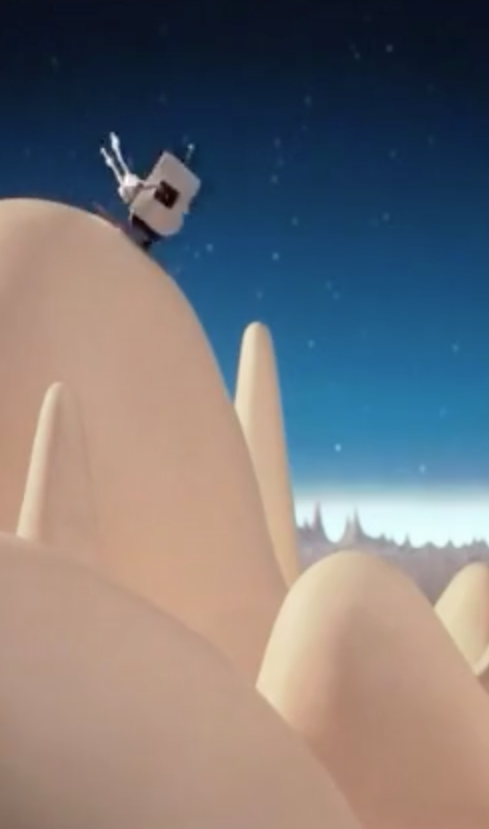
\includegraphics[width=4in]{primer}};
        \begin{scope}[scale=2.5, line width=5pt]
          \draw[{Latex[scale=1]}-] (-1,1.2) -- (-1, -3);
          \node at (-0.4, -1) {$U\left(\vec{q}\right)$};
          \draw[-{Latex[scale=1]}] (-2,-3.2) -- (2, -3.2);
          \node at (0, -2.9) {$\vec{q}$};
          \draw[-{Latex[scale=1]},white] (-0.5,1.5) -- (0, 1);
          \node[white] at (0.8, 1.35) {$\vec{p}=\mat{M}\vec{v}$};
          \node[white] at (0, 3) {$K\left(\vec{p}\right) = \frac{1}{2}\vec{p}^T \mat{M}^{-1} \vec{p}$};
        \end{scope}
      \end{tikzpicture}
    \end{multicols*}
  }

  \block{Hamiltonian Monte Carlo}{

    \flushleft

    Hamiltonian Monte Carlo (HMC) is a statistical technique that harnesses physical laws to efficiently sample complex distributions [2].
    To do so, we construct the ski slope as follows:
    \begin{itemize}
      \item Every location $\vec{q}$ maps to some tree and branch lengths
      \item The elevation at point $\vec{q}$ is $-\log{P\left(\mathcal{T}\mid D\right)}$
      \begin{itemize}
        \item Locations with \textbf{high elevation} have \textbf{low probability}
        \item Locations with \textbf{low elevation} have \textbf{high probability}
      \end{itemize}
    \end{itemize}
    We can only approximately simulate the robot's motion with a numerical integrator.

    \bigskip

    However, vanilla HMC \textbf{does not currently work for phylogenetics}.
    To extend HMC to the \textbf{space of phylogenetic trees} we use the following ideas:

    \vspace{-96pt}

    \innerblock{Billera--Holmes\\--Vogtmann\\Tree Space [1]}{
      \flushleft
      \begin{itemize}
        \item Each topology is represented by a \textbf{hypercube} containing all possible choices of branch lengths
        \item By \textbf{collapsing an internal branch length} to 0 and re-expanding it differently, we can change a tree to one of its \textbf{NNI neighbors}
        \item Thus we can ``glue'' the tree-cubes together into a \textbf{single space}
      \end{itemize}
    }

    \vspace{-96pt}

    \innerblock{Leap-Prog Integrator}{
      \flushleft
      \begin{itemize}
        \item Because every boundary is \textbf{shared between 3 trees}, there is no deterministic path for the robot to follow
        \item Introduce a \textbf{probabilistic simulator} that chooses randomly between neighboring trees at the boundary
      \end{itemize}
    }

    \vspace{-96pt}

    \innerblock{Surrogate Hamiltonian}{
      \flushleft
      \begin{itemize}
        \item At between-tree boundaries, the ski slope forms \textbf{sharp peaks}
        \item \textbf{Difficult} to accurately simulate robot's motion at these peaks
        \item Substitute a surrogate $\mathcal{H}^\prime$ that artificially \textbf{smooths} the peaks
      \end{itemize}
    }

  }

  \block{Example: 4 taxa}{
    \centering
    \vspace{-0.5in}
    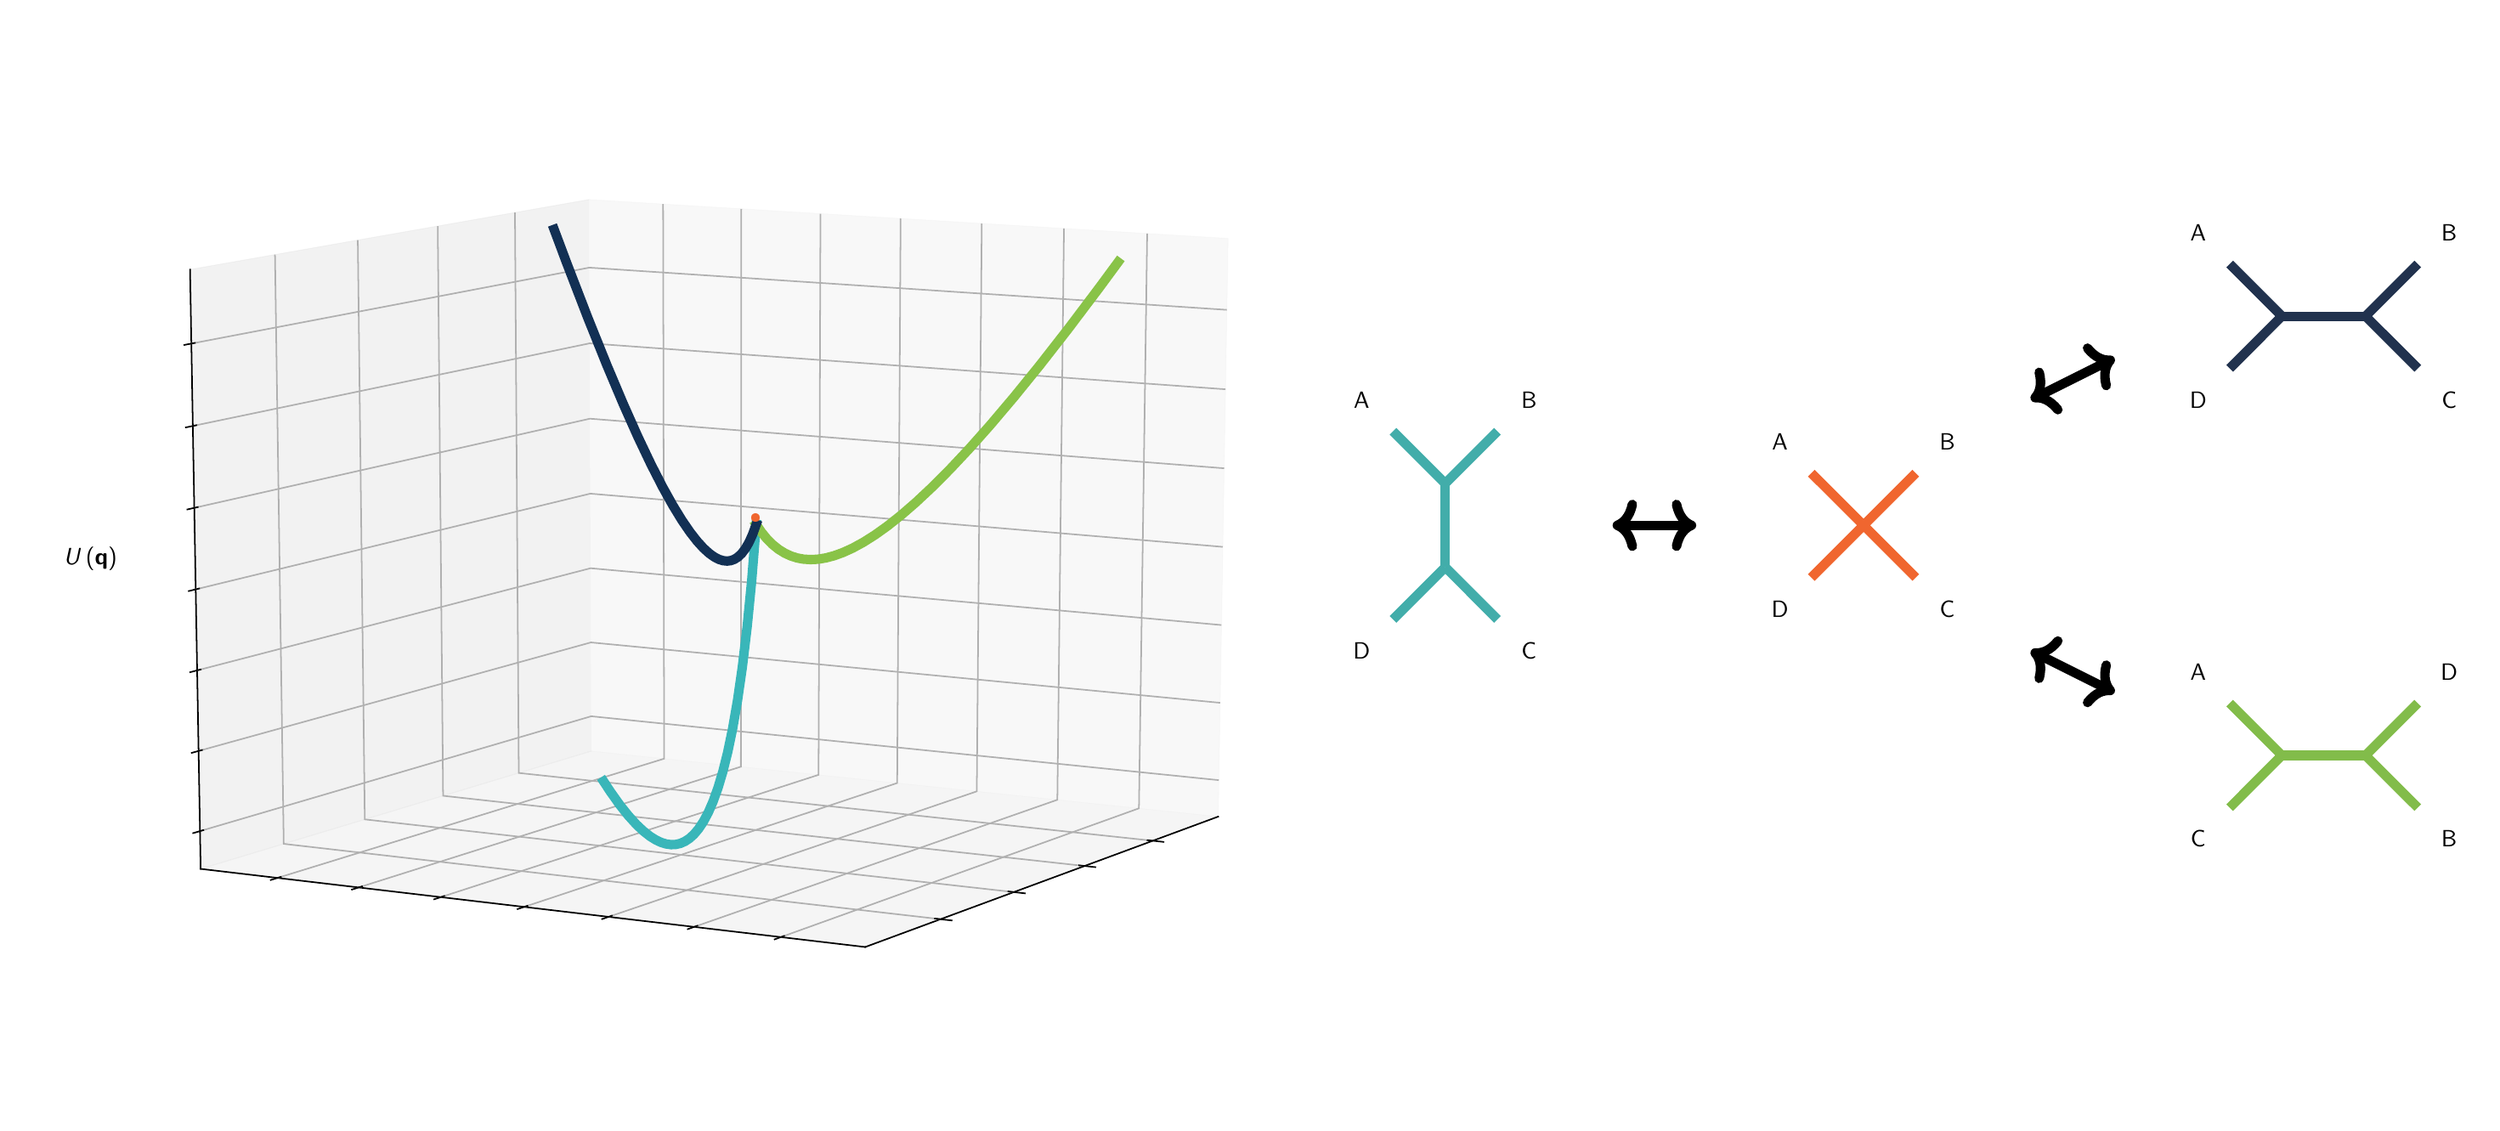
\begin{tikzpicture}
      \begin{scope}[scale=1.25,line width=4pt,shift={(22,-6)}]
        \begin{scope}[minimum size=8mm]
          \node [label=center:A] (0) at (-1, 1) {};
          \node [label=center:C] (1) at (1, -1) {};
          \node [label=center:B] (2) at (1, 1) {};
          \node [label=center:D] (3) at (-1, -1) {};
          \node [] (4) at (-2, 0) {};
          \node [] (5) at (-3, 0) {};
          \node [label=center:C] (6) at (-4, -1.5) {};
          \node [label=center:D] (7) at (-6, -1.5) {};
          \node [] (8) at (-5, -0.5) {};
          \node [] (9) at (-5, 0.5) {};
          \node [label=center:A] (10) at (-6, 1.5) {};
          \node [label=center:B] (11) at (-4, 1.5) {};
          \node [] (12) at (2, 1.5) {};
          \node [] (13) at (3, 2) {};
          \node [] (14) at (2, -1.5) {};
          \node [] (15) at (3, -2) {};
          \begin{scope}[shift={(0,-1)}]
            \node [label=center:A] (16) at (4, -0.75) {};
            \node [label=center:C] (17) at (4, -2.75) {};
            \node [] (18) at (5, -1.75) {};
            \node [] (19) at (6, -1.75) {};
            \node [label=center:B] (20) at (7, -2.75) {};
            \node [label=center:D] (21) at (7, -0.75) {};
          \end{scope}
          \begin{scope}[shift={(0,1)}]
            \node [label=center:D] (22) at (4, 0.5) {};
            \node [label=center:A] (23) at (4, 2.5) {};
            \node [] (24) at (5, 1.5) {};
            \node [] (25) at (6, 1.5) {};
            \node [label=center:C] (26) at (7, 0.5) {};
            \node [label=center:B] (27) at (7, 2.5) {};
          \end{scope}
        \end{scope}
        \draw[fhorange] (0.south east) to (1);
        \draw[fhorange] (2) to (3);
        \draw [<->] (4.center) to (5.center);
        \draw[fhturq] (10) to (9.center);
        \draw[fhturq] (9.center) to (8.center);
        \draw[fhturq] (8.center) to (7);
        \draw[fhturq] (8.center) to (6);
        \draw[fhturq] (9.center) to (11);
        \draw [<->] (14.center) to (15.center);
        \draw [<->] (12.center) to (13.center);
        \draw[fhnavy] (22) to (24.center);
        \draw[fhnavy] (24.center) to (25.center);
        \draw[fhnavy] (25.center) to (26);
        \draw[fhnavy] (25.center) to (27);
        \draw[fhnavy] (24.center) to (23);
        \draw[fhgreen] (16) to (18.center);
        \draw[fhgreen] (18.center) to (17);
        \draw[fhgreen] (18.center) to (19.center);
        \draw[fhgreen] (19.center) to (20);
        \draw[fhgreen] (19.center) to (21);
      \end{scope}
      \begin{scope}[scale=2]
        \definecolor{cf2f2f2}{RGB}{242,242,242}
\definecolor{ce6e6e6}{RGB}{230,230,230}
\definecolor{cececec}{RGB}{236,236,236}
\definecolor{cb0b0b0}{RGB}{176,176,176}
\definecolor{c39b6b9}{RGB}{57,182,185}
\definecolor{c89c348}{RGB}{137,195,72}
\definecolor{c123054}{RGB}{18,48,84}


\begin{scope}[y=0.80pt, x=0.80pt, yscale=-1.000000, xscale=1.000000, inner sep=0pt, outer sep=0pt]
    \path (0.0000,288.0000) -- (360.0000,288.0000) -- (360.0000,0.0000) --
      (0.0000,0.0000) -- cycle;
    \path (2.5200,285.4800) -- (357.4800,285.4800) -- (357.4800,2.5200) --
      (2.5200,2.5200) -- cycle;
      \path[draw=cf2f2f2,fill=cf2f2f2,opacity=0.500,line join=miter]
        (150.9214,193.3673) -- (317.5047,210.7879) -- (320.1195,57.1427) --
        (150.2862,46.8068);
      \path[draw=ce6e6e6,fill=ce6e6e6,opacity=0.500,line join=miter]
        (150.9214,193.3673) -- (47.0780,224.6800) -- (44.2599,65.3989) --
        (150.2862,46.8068);
      \path[draw=cececec,fill=cececec,opacity=0.500,line join=miter]
        (150.9214,193.3673) -- (47.0780,224.6800) -- (223.7053,245.4445) --
        (317.5047,210.7879);
      \path[draw=black,line cap=rect,line width=0.640pt] (317.5047,210.7879) --
        (223.7053,245.4445);
      \path[draw=cb0b0b0,line width=0.640pt] (300.1369,217.2049) --
        (131.6241,199.1862) -- (130.6101,50.2570);
      \path[draw=cb0b0b0,line width=0.640pt] (282.0034,223.9048) --
        (111.5099,205.2514) -- (110.0881,53.8556);
      \path[draw=cb0b0b0,line width=0.640pt] (263.2089,230.8489) -- (90.6991,211.5266)
        -- (88.8413,57.5814);
      \path[draw=cb0b0b0,line width=0.640pt] (243.7167,238.0507) -- (69.1548,218.0230)
        -- (66.8306,61.4410);
        \path[draw=black,line cap=rect,line width=0.640pt] (298.7212,217.0535) --
          (302.9718,217.5080);
        \path[draw=black,line cap=rect,line width=0.640pt] (280.5698,223.7479) --
          (284.8741,224.2189);
        \path[draw=black,line cap=rect,line width=0.640pt] (261.7571,230.6863) --
          (266.1162,231.1745);
        \path[draw=black,line cap=rect,line width=0.640pt] (242.2463,237.8820) --
          (246.6614,238.3886);
      \path[draw=black,line cap=rect,line width=0.640pt] (47.0780,224.6800) --
        (223.7053,245.4445);
      \path[draw=cb0b0b0,line width=0.640pt] (169.9843,48.0056) -- (170.2585,195.3895)
        -- (67.5004,227.0809);
      \path[draw=cb0b0b0,line width=0.640pt] (190.7648,49.2702) -- (190.6536,197.5224)
        -- (89.0632,229.6158);
      \path[draw=cb0b0b0,line width=0.640pt] (211.8032,50.5506) -- (211.2971,199.6812)
        -- (110.9124,232.1844);
      \path[draw=cb0b0b0,line width=0.640pt] (233.1042,51.8470) -- (232.1934,201.8664)
        -- (133.0537,234.7874);
      \path[draw=cb0b0b0,line width=0.640pt] (254.6727,53.1596) -- (253.3472,204.0786)
        -- (155.4932,237.4254);
      \path[draw=cb0b0b0,line width=0.640pt] (276.5140,54.4889) -- (274.7633,206.3182)
        -- (178.2367,240.0992);
      \path[draw=cb0b0b0,line width=0.640pt] (298.6331,55.8350) -- (296.4467,208.5858)
        -- (201.2906,242.8094);
        \path[draw=black,line cap=rect,line width=0.640pt] (68.3957,226.8048) --
          (65.7059,227.6343);
        \path[draw=black,line cap=rect,line width=0.640pt] (89.9488,229.3361) --
          (87.2881,230.1766);
        \path[draw=black,line cap=rect,line width=0.640pt] (111.7880,231.9009) --
          (109.1574,232.7527);
        \path[draw=black,line cap=rect,line width=0.640pt] (133.9190,234.5001) --
          (131.3195,235.3633);
        \path[draw=black,line cap=rect,line width=0.640pt] (156.3477,237.1342) --
          (153.7804,238.0091);
        \path[draw=black,line cap=rect,line width=0.640pt] (179.0801,239.8040) --
          (176.5463,240.6908);
        \path[draw=black,line cap=rect,line width=0.640pt] (202.1225,242.5102) --
          (199.6232,243.4091);
      \path[draw=black,line cap=rect,line width=0.640pt] (47.0780,224.6800) --
        (44.2599,65.3989);
      \path[draw=cb0b0b0,line width=0.640pt] (46.9003,214.6412) -- (150.8813,184.1158)
        -- (317.6696,201.0976);
      \path[draw=cb0b0b0,line width=0.640pt] (46.5235,193.3405) -- (150.7963,164.4918)
        -- (318.0195,180.5393);
      \path[draw=cb0b0b0,line width=0.640pt] (46.1446,171.9231) -- (150.7108,144.7692)
        -- (318.3712,159.8724);
      \path[draw=cb0b0b0,line width=0.640pt] (45.7636,150.3879) -- (150.6249,124.9472)
        -- (318.7248,139.0961);
      \path[draw=cb0b0b0,line width=0.640pt] (45.3805,128.7341) -- (150.5385,105.0250)
        -- (319.0802,118.2095);
      \path[draw=cb0b0b0,line width=0.640pt] (44.9952,106.9606) -- (150.4518,85.0019)
        -- (319.4376,97.2118);
      \path[draw=cb0b0b0,line width=0.640pt] (44.6079,85.0665) -- (150.3645,64.8771)
        -- (319.7968,76.1020);
        \path[draw=black,line cap=rect,line width=0.640pt] (47.8060,214.3754) --
          (45.0852,215.1741);
        \begin{scope}[shift={(17.85289,223.21522)},xscale=0.100,yscale=-0.100]
            \path (31.7812,34.6250) .. controls (27.0938,34.6250) and (23.4062,33.3698) ..
              (20.7188,30.8594) .. controls (18.0417,28.3490) and (16.7031,24.9010) ..
              (16.7031,20.5156) .. controls (16.7031,16.1198) and (18.0417,12.6667) ..
              (20.7188,10.1562) .. controls (23.4062,7.6458) and (27.0938,6.3906) ..
              (31.7812,6.3906) .. controls (36.4688,6.3906) and (40.1615,7.6510) ..
              (42.8594,10.1719) .. controls (45.5677,12.7031) and (46.9219,16.1510) ..
              (46.9219,20.5156) .. controls (46.9219,24.9010) and (45.5781,28.3490) ..
              (42.8906,30.8594) .. controls (40.2135,33.3698) and (36.5104,34.6250) ..
              (31.7812,34.6250)(21.9219,38.8125) .. controls (17.6927,39.8542) and
              (14.3958,41.8229) .. (12.0312,44.7188) .. controls (9.6771,47.6250) and
              (8.5000,51.1615) .. (8.5000,55.3281) .. controls (8.5000,61.1510) and
              (10.5729,65.7552) .. (14.7188,69.1406) .. controls (18.8750,72.5260) and
              (24.5625,74.2188) .. (31.7812,74.2188) .. controls (39.0417,74.2188) and
              (44.7396,72.5260) .. (48.8750,69.1406) .. controls (53.0104,65.7552) and
              (55.0781,61.1510) .. (55.0781,55.3281) .. controls (55.0781,51.1615) and
              (53.8958,47.6250) .. (51.5312,44.7188) .. controls (49.1771,41.8229) and
              (45.9010,39.8542) .. (41.7031,38.8125) .. controls (46.4531,37.7083) and
              (50.1510,35.5417) .. (52.7969,32.3125) .. controls (55.4531,29.0938) and
              (56.7812,25.1615) .. (56.7812,20.5156) .. controls (56.7812,13.4427) and
              (54.6250,8.0156) .. (50.3125,4.2344) .. controls (46.0000,0.4635) and
              (39.8229,-1.4219) .. (31.7812,-1.4219) .. controls (23.7500,-1.4219) and
              (17.5729,0.4635) .. (13.2500,4.2344) .. controls (8.9375,8.0156) and
              (6.7812,13.4427) .. (6.7812,20.5156) .. controls (6.7812,25.1615) and
              (8.1146,29.0938) .. (10.7812,32.3125) .. controls (13.4583,35.5417) and
              (17.1719,37.7083) .. (21.9219,38.8125)(18.3125,54.3906) .. controls
              (18.3125,50.6198) and (19.4896,47.6771) .. (21.8438,45.5625) .. controls
              (24.2083,43.4479) and (27.5208,42.3906) .. (31.7812,42.3906) .. controls
              (36.0208,42.3906) and (39.3333,43.4479) .. (41.7188,45.5625) .. controls
              (44.1146,47.6771) and (45.3125,50.6198) .. (45.3125,54.3906) .. controls
              (45.3125,58.1719) and (44.1146,61.1198) .. (41.7188,63.2344) .. controls
              (39.3333,65.3490) and (36.0208,66.4062) .. (31.7812,66.4062) .. controls
              (27.5208,66.4062) and (24.2083,65.3490) .. (21.8438,63.2344) .. controls
              (19.4896,61.1198) and (18.3125,58.1719) .. (18.3125,54.3906);
          \begin{scope}[shift={(63.62305,0)}]
            \path (10.7969,72.9062) -- (49.5156,72.9062) -- (49.5156,64.5938) --
              (19.8281,64.5938) -- (19.8281,46.7344) .. controls (21.2552,47.2240) and
              (22.6823,47.5885) .. (24.1094,47.8281) .. controls (25.5469,48.0677) and
              (26.9844,48.1875) .. (28.4219,48.1875) .. controls (36.5573,48.1875) and
              (43.0000,45.9583) .. (47.7500,41.5000) .. controls (52.5104,37.0417) and
              (54.8906,31.0052) .. (54.8906,23.3906) .. controls (54.8906,15.5469) and
              (52.4479,9.4479) .. (47.5625,5.0938) .. controls (42.6771,0.7500) and
              (35.7917,-1.4219) .. (26.9062,-1.4219) .. controls (23.8438,-1.4219) and
              (20.7240,-1.1615) .. (17.5469,-0.6406) .. controls (14.3802,-0.1198) and
              (11.1042,0.6615) .. (7.7188,1.7031) -- (7.7188,11.6250) .. controls
              (10.6458,10.0312) and (13.6719,8.8438) .. (16.7969,8.0625) .. controls
              (19.9219,7.2812) and (23.2240,6.8906) .. (26.7031,6.8906) .. controls
              (32.3385,6.8906) and (36.7969,8.3698) .. (40.0781,11.3281) .. controls
              (43.3698,14.2865) and (45.0156,18.3073) .. (45.0156,23.3906) .. controls
              (45.0156,28.4635) and (43.3698,32.4792) .. (40.0781,35.4375) .. controls
              (36.7969,38.4062) and (32.3385,39.8906) .. (26.7031,39.8906) .. controls
              (24.0677,39.8906) and (21.4375,39.5990) .. (18.8125,39.0156) .. controls
              (16.1979,38.4323) and (13.5260,37.5208) .. (10.7969,36.2812) -- cycle;
          \end{scope}
          \begin{scope}[shift={(127.24609,0)}]
            \path (31.7812,34.6250) .. controls (27.0938,34.6250) and (23.4062,33.3698) ..
              (20.7188,30.8594) .. controls (18.0417,28.3490) and (16.7031,24.9010) ..
              (16.7031,20.5156) .. controls (16.7031,16.1198) and (18.0417,12.6667) ..
              (20.7188,10.1562) .. controls (23.4062,7.6458) and (27.0938,6.3906) ..
              (31.7812,6.3906) .. controls (36.4688,6.3906) and (40.1615,7.6510) ..
              (42.8594,10.1719) .. controls (45.5677,12.7031) and (46.9219,16.1510) ..
              (46.9219,20.5156) .. controls (46.9219,24.9010) and (45.5781,28.3490) ..
              (42.8906,30.8594) .. controls (40.2135,33.3698) and (36.5104,34.6250) ..
              (31.7812,34.6250)(21.9219,38.8125) .. controls (17.6927,39.8542) and
              (14.3958,41.8229) .. (12.0312,44.7188) .. controls (9.6771,47.6250) and
              (8.5000,51.1615) .. (8.5000,55.3281) .. controls (8.5000,61.1510) and
              (10.5729,65.7552) .. (14.7188,69.1406) .. controls (18.8750,72.5260) and
              (24.5625,74.2188) .. (31.7812,74.2188) .. controls (39.0417,74.2188) and
              (44.7396,72.5260) .. (48.8750,69.1406) .. controls (53.0104,65.7552) and
              (55.0781,61.1510) .. (55.0781,55.3281) .. controls (55.0781,51.1615) and
              (53.8958,47.6250) .. (51.5312,44.7188) .. controls (49.1771,41.8229) and
              (45.9010,39.8542) .. (41.7031,38.8125) .. controls (46.4531,37.7083) and
              (50.1510,35.5417) .. (52.7969,32.3125) .. controls (55.4531,29.0938) and
              (56.7812,25.1615) .. (56.7812,20.5156) .. controls (56.7812,13.4427) and
              (54.6250,8.0156) .. (50.3125,4.2344) .. controls (46.0000,0.4635) and
              (39.8229,-1.4219) .. (31.7812,-1.4219) .. controls (23.7500,-1.4219) and
              (17.5729,0.4635) .. (13.2500,4.2344) .. controls (8.9375,8.0156) and
              (6.7812,13.4427) .. (6.7812,20.5156) .. controls (6.7812,25.1615) and
              (8.1146,29.0938) .. (10.7812,32.3125) .. controls (13.4583,35.5417) and
              (17.1719,37.7083) .. (21.9219,38.8125)(18.3125,54.3906) .. controls
              (18.3125,50.6198) and (19.4896,47.6771) .. (21.8438,45.5625) .. controls
              (24.2083,43.4479) and (27.5208,42.3906) .. (31.7812,42.3906) .. controls
              (36.0208,42.3906) and (39.3333,43.4479) .. (41.7188,45.5625) .. controls
              (44.1146,47.6771) and (45.3125,50.6198) .. (45.3125,54.3906) .. controls
              (45.3125,58.1719) and (44.1146,61.1198) .. (41.7188,63.2344) .. controls
              (39.3333,65.3490) and (36.0208,66.4062) .. (31.7812,66.4062) .. controls
              (27.5208,66.4062) and (24.2083,65.3490) .. (21.8438,63.2344) .. controls
              (19.4896,61.1198) and (18.3125,58.1719) .. (18.3125,54.3906);
          \end{scope}
        \end{scope}
        \path[draw=black,line cap=rect,line width=0.640pt] (47.4318,193.0892) --
          (44.7029,193.8442);
        \begin{scope}[shift={(17.4216,201.86114)},xscale=0.100,yscale=-0.100]
            \path (31.7812,34.6250) .. controls (27.0938,34.6250) and (23.4062,33.3698) ..
              (20.7188,30.8594) .. controls (18.0417,28.3490) and (16.7031,24.9010) ..
              (16.7031,20.5156) .. controls (16.7031,16.1198) and (18.0417,12.6667) ..
              (20.7188,10.1562) .. controls (23.4062,7.6458) and (27.0938,6.3906) ..
              (31.7812,6.3906) .. controls (36.4688,6.3906) and (40.1615,7.6510) ..
              (42.8594,10.1719) .. controls (45.5677,12.7031) and (46.9219,16.1510) ..
              (46.9219,20.5156) .. controls (46.9219,24.9010) and (45.5781,28.3490) ..
              (42.8906,30.8594) .. controls (40.2135,33.3698) and (36.5104,34.6250) ..
              (31.7812,34.6250)(21.9219,38.8125) .. controls (17.6927,39.8542) and
              (14.3958,41.8229) .. (12.0312,44.7188) .. controls (9.6771,47.6250) and
              (8.5000,51.1615) .. (8.5000,55.3281) .. controls (8.5000,61.1510) and
              (10.5729,65.7552) .. (14.7188,69.1406) .. controls (18.8750,72.5260) and
              (24.5625,74.2188) .. (31.7812,74.2188) .. controls (39.0417,74.2188) and
              (44.7396,72.5260) .. (48.8750,69.1406) .. controls (53.0104,65.7552) and
              (55.0781,61.1510) .. (55.0781,55.3281) .. controls (55.0781,51.1615) and
              (53.8958,47.6250) .. (51.5312,44.7188) .. controls (49.1771,41.8229) and
              (45.9010,39.8542) .. (41.7031,38.8125) .. controls (46.4531,37.7083) and
              (50.1510,35.5417) .. (52.7969,32.3125) .. controls (55.4531,29.0938) and
              (56.7812,25.1615) .. (56.7812,20.5156) .. controls (56.7812,13.4427) and
              (54.6250,8.0156) .. (50.3125,4.2344) .. controls (46.0000,0.4635) and
              (39.8229,-1.4219) .. (31.7812,-1.4219) .. controls (23.7500,-1.4219) and
              (17.5729,0.4635) .. (13.2500,4.2344) .. controls (8.9375,8.0156) and
              (6.7812,13.4427) .. (6.7812,20.5156) .. controls (6.7812,25.1615) and
              (8.1146,29.0938) .. (10.7812,32.3125) .. controls (13.4583,35.5417) and
              (17.1719,37.7083) .. (21.9219,38.8125)(18.3125,54.3906) .. controls
              (18.3125,50.6198) and (19.4896,47.6771) .. (21.8438,45.5625) .. controls
              (24.2083,43.4479) and (27.5208,42.3906) .. (31.7812,42.3906) .. controls
              (36.0208,42.3906) and (39.3333,43.4479) .. (41.7188,45.5625) .. controls
              (44.1146,47.6771) and (45.3125,50.6198) .. (45.3125,54.3906) .. controls
              (45.3125,58.1719) and (44.1146,61.1198) .. (41.7188,63.2344) .. controls
              (39.3333,65.3490) and (36.0208,66.4062) .. (31.7812,66.4062) .. controls
              (27.5208,66.4062) and (24.2083,65.3490) .. (21.8438,63.2344) .. controls
              (19.4896,61.1198) and (18.3125,58.1719) .. (18.3125,54.3906);
          \begin{scope}[shift={(63.62305,0)}]
            \path (33.0156,40.3750) .. controls (28.5885,40.3750) and (25.0781,38.8594) ..
              (22.4844,35.8281) .. controls (19.9010,32.8073) and (18.6094,28.6615) ..
              (18.6094,23.3906) .. controls (18.6094,18.1510) and (19.9010,14.0052) ..
              (22.4844,10.9531) .. controls (25.0781,7.9115) and (28.5885,6.3906) ..
              (33.0156,6.3906) .. controls (37.4427,6.3906) and (40.9479,7.9115) ..
              (43.5312,10.9531) .. controls (46.1146,14.0052) and (47.4062,18.1510) ..
              (47.4062,23.3906) .. controls (47.4062,28.6615) and (46.1146,32.8073) ..
              (43.5312,35.8281) .. controls (40.9479,38.8594) and (37.4427,40.3750) ..
              (33.0156,40.3750)(52.5938,71.2969) -- (52.5938,62.3125) .. controls
              (50.1146,63.4792) and (47.6146,64.3698) .. (45.0938,64.9844) .. controls
              (42.5729,65.6094) and (40.0729,65.9219) .. (37.5938,65.9219) .. controls
              (31.0833,65.9219) and (26.1094,63.7240) .. (22.6719,59.3281) .. controls
              (19.2448,54.9323) and (17.2865,48.2917) .. (16.7969,39.4062) .. controls
              (18.7135,42.2396) and (21.1198,44.4115) .. (24.0156,45.9219) .. controls
              (26.9219,47.4323) and (30.1146,48.1875) .. (33.5938,48.1875) .. controls
              (40.9167,48.1875) and (46.7031,45.9635) .. (50.9531,41.5156) .. controls
              (55.2031,37.0781) and (57.3281,31.0365) .. (57.3281,23.3906) .. controls
              (57.3281,15.9010) and (55.1146,9.8906) .. (50.6875,5.3594) .. controls
              (46.2604,0.8385) and (40.3698,-1.4219) .. (33.0156,-1.4219) .. controls
              (24.5781,-1.4219) and (18.1302,1.8073) .. (13.6719,8.2656) .. controls
              (9.2135,14.7344) and (6.9844,24.1042) .. (6.9844,36.3750) .. controls
              (6.9844,47.8958) and (9.7188,57.0833) .. (15.1875,63.9375) .. controls
              (20.6562,70.7917) and (27.9948,74.2188) .. (37.2031,74.2188) .. controls
              (39.6823,74.2188) and (42.1823,73.9740) .. (44.7031,73.4844) .. controls
              (47.2240,72.9948) and (49.8542,72.2656) .. (52.5938,71.2969);
          \end{scope}
          \begin{scope}[shift={(127.24609,0)}]
            \path (31.7812,66.4062) .. controls (26.7083,66.4062) and (22.8906,63.9062) ..
              (20.3281,58.9062) .. controls (17.7760,53.9167) and (16.5000,46.4062) ..
              (16.5000,36.3750) .. controls (16.5000,26.3854) and (17.7760,18.8906) ..
              (20.3281,13.8906) .. controls (22.8906,8.8906) and (26.7083,6.3906) ..
              (31.7812,6.3906) .. controls (36.8958,6.3906) and (40.7292,8.8906) ..
              (43.2812,13.8906) .. controls (45.8438,18.8906) and (47.1250,26.3854) ..
              (47.1250,36.3750) .. controls (47.1250,46.4062) and (45.8438,53.9167) ..
              (43.2812,58.9062) .. controls (40.7292,63.9062) and (36.8958,66.4062) ..
              (31.7812,66.4062)(31.7812,74.2188) .. controls (39.9583,74.2188) and
              (46.2031,70.9844) .. (50.5156,64.5156) .. controls (54.8281,58.0573) and
              (56.9844,48.6771) .. (56.9844,36.3750) .. controls (56.9844,24.1042) and
              (54.8281,14.7344) .. (50.5156,8.2656) .. controls (46.2031,1.8073) and
              (39.9583,-1.4219) .. (31.7812,-1.4219) .. controls (23.6146,-1.4219) and
              (17.3750,1.8073) .. (13.0625,8.2656) .. controls (8.7500,14.7344) and
              (6.5938,24.1042) .. (6.5938,36.3750) .. controls (6.5938,48.6771) and
              (8.7500,58.0573) .. (13.0625,64.5156) .. controls (17.3750,70.9844) and
              (23.6146,74.2188) .. (31.7812,74.2188);
          \end{scope}
        \end{scope}
        \path[draw=black,line cap=rect,line width=0.640pt] (47.0557,171.6865) --
          (44.3184,172.3973);
        \begin{scope}[shift={(16.98794,180.38972)},xscale=0.100,yscale=-0.100]
            \path (31.7812,34.6250) .. controls (27.0938,34.6250) and (23.4062,33.3698) ..
              (20.7188,30.8594) .. controls (18.0417,28.3490) and (16.7031,24.9010) ..
              (16.7031,20.5156) .. controls (16.7031,16.1198) and (18.0417,12.6667) ..
              (20.7188,10.1562) .. controls (23.4062,7.6458) and (27.0938,6.3906) ..
              (31.7812,6.3906) .. controls (36.4688,6.3906) and (40.1615,7.6510) ..
              (42.8594,10.1719) .. controls (45.5677,12.7031) and (46.9219,16.1510) ..
              (46.9219,20.5156) .. controls (46.9219,24.9010) and (45.5781,28.3490) ..
              (42.8906,30.8594) .. controls (40.2135,33.3698) and (36.5104,34.6250) ..
              (31.7812,34.6250)(21.9219,38.8125) .. controls (17.6927,39.8542) and
              (14.3958,41.8229) .. (12.0312,44.7188) .. controls (9.6771,47.6250) and
              (8.5000,51.1615) .. (8.5000,55.3281) .. controls (8.5000,61.1510) and
              (10.5729,65.7552) .. (14.7188,69.1406) .. controls (18.8750,72.5260) and
              (24.5625,74.2188) .. (31.7812,74.2188) .. controls (39.0417,74.2188) and
              (44.7396,72.5260) .. (48.8750,69.1406) .. controls (53.0104,65.7552) and
              (55.0781,61.1510) .. (55.0781,55.3281) .. controls (55.0781,51.1615) and
              (53.8958,47.6250) .. (51.5312,44.7188) .. controls (49.1771,41.8229) and
              (45.9010,39.8542) .. (41.7031,38.8125) .. controls (46.4531,37.7083) and
              (50.1510,35.5417) .. (52.7969,32.3125) .. controls (55.4531,29.0938) and
              (56.7812,25.1615) .. (56.7812,20.5156) .. controls (56.7812,13.4427) and
              (54.6250,8.0156) .. (50.3125,4.2344) .. controls (46.0000,0.4635) and
              (39.8229,-1.4219) .. (31.7812,-1.4219) .. controls (23.7500,-1.4219) and
              (17.5729,0.4635) .. (13.2500,4.2344) .. controls (8.9375,8.0156) and
              (6.7812,13.4427) .. (6.7812,20.5156) .. controls (6.7812,25.1615) and
              (8.1146,29.0938) .. (10.7812,32.3125) .. controls (13.4583,35.5417) and
              (17.1719,37.7083) .. (21.9219,38.8125)(18.3125,54.3906) .. controls
              (18.3125,50.6198) and (19.4896,47.6771) .. (21.8438,45.5625) .. controls
              (24.2083,43.4479) and (27.5208,42.3906) .. (31.7812,42.3906) .. controls
              (36.0208,42.3906) and (39.3333,43.4479) .. (41.7188,45.5625) .. controls
              (44.1146,47.6771) and (45.3125,50.6198) .. (45.3125,54.3906) .. controls
              (45.3125,58.1719) and (44.1146,61.1198) .. (41.7188,63.2344) .. controls
              (39.3333,65.3490) and (36.0208,66.4062) .. (31.7812,66.4062) .. controls
              (27.5208,66.4062) and (24.2083,65.3490) .. (21.8438,63.2344) .. controls
              (19.4896,61.1198) and (18.3125,58.1719) .. (18.3125,54.3906);
          \begin{scope}[shift={(63.62305,0)}]
            \path (33.0156,40.3750) .. controls (28.5885,40.3750) and (25.0781,38.8594) ..
              (22.4844,35.8281) .. controls (19.9010,32.8073) and (18.6094,28.6615) ..
              (18.6094,23.3906) .. controls (18.6094,18.1510) and (19.9010,14.0052) ..
              (22.4844,10.9531) .. controls (25.0781,7.9115) and (28.5885,6.3906) ..
              (33.0156,6.3906) .. controls (37.4427,6.3906) and (40.9479,7.9115) ..
              (43.5312,10.9531) .. controls (46.1146,14.0052) and (47.4062,18.1510) ..
              (47.4062,23.3906) .. controls (47.4062,28.6615) and (46.1146,32.8073) ..
              (43.5312,35.8281) .. controls (40.9479,38.8594) and (37.4427,40.3750) ..
              (33.0156,40.3750)(52.5938,71.2969) -- (52.5938,62.3125) .. controls
              (50.1146,63.4792) and (47.6146,64.3698) .. (45.0938,64.9844) .. controls
              (42.5729,65.6094) and (40.0729,65.9219) .. (37.5938,65.9219) .. controls
              (31.0833,65.9219) and (26.1094,63.7240) .. (22.6719,59.3281) .. controls
              (19.2448,54.9323) and (17.2865,48.2917) .. (16.7969,39.4062) .. controls
              (18.7135,42.2396) and (21.1198,44.4115) .. (24.0156,45.9219) .. controls
              (26.9219,47.4323) and (30.1146,48.1875) .. (33.5938,48.1875) .. controls
              (40.9167,48.1875) and (46.7031,45.9635) .. (50.9531,41.5156) .. controls
              (55.2031,37.0781) and (57.3281,31.0365) .. (57.3281,23.3906) .. controls
              (57.3281,15.9010) and (55.1146,9.8906) .. (50.6875,5.3594) .. controls
              (46.2604,0.8385) and (40.3698,-1.4219) .. (33.0156,-1.4219) .. controls
              (24.5781,-1.4219) and (18.1302,1.8073) .. (13.6719,8.2656) .. controls
              (9.2135,14.7344) and (6.9844,24.1042) .. (6.9844,36.3750) .. controls
              (6.9844,47.8958) and (9.7188,57.0833) .. (15.1875,63.9375) .. controls
              (20.6562,70.7917) and (27.9948,74.2188) .. (37.2031,74.2188) .. controls
              (39.6823,74.2188) and (42.1823,73.9740) .. (44.7031,73.4844) .. controls
              (47.2240,72.9948) and (49.8542,72.2656) .. (52.5938,71.2969);
          \end{scope}
          \begin{scope}[shift={(127.24609,0)}]
            \path (19.1875,8.2969) -- (53.6094,8.2969) -- (53.6094,0.0000) --
              (7.3281,0.0000) -- (7.3281,8.2969) .. controls (11.0677,12.1719) and
              (16.1667,17.3698) .. (22.6250,23.8906) .. controls (29.0938,30.4219) and
              (33.1562,34.6354) .. (34.8125,36.5312) .. controls (37.9688,40.0729) and
              (40.1719,43.0729) .. (41.4219,45.5312) .. controls (42.6823,47.9896) and
              (43.3125,50.4062) .. (43.3125,52.7812) .. controls (43.3125,56.6562) and
              (41.9531,59.8125) .. (39.2344,62.2500) .. controls (36.5156,64.6979) and
              (32.9740,65.9219) .. (28.6094,65.9219) .. controls (25.5156,65.9219) and
              (22.2500,65.3854) .. (18.8125,64.3125) .. controls (15.3854,63.2396) and
              (11.7188,61.6094) .. (7.8125,59.4219) -- (7.8125,69.3906) .. controls
              (11.7812,70.9844) and (15.4896,72.1875) .. (18.9375,73.0000) .. controls
              (22.3958,73.8125) and (25.5573,74.2188) .. (28.4219,74.2188) .. controls
              (35.9740,74.2188) and (41.9948,72.3281) .. (46.4844,68.5469) .. controls
              (50.9740,64.7760) and (53.2188,59.7344) .. (53.2188,53.4219) .. controls
              (53.2188,50.4219) and (52.6562,47.5781) .. (51.5312,44.8906) .. controls
              (50.4167,42.2135) and (48.3750,39.0521) .. (45.4062,35.4062) .. controls
              (44.5938,34.4583) and (42.0052,31.7292) .. (37.6406,27.2188) .. controls
              (33.2865,22.7083) and (27.1354,16.4010) .. (19.1875,8.2969);
          \end{scope}
        \end{scope}
        \path[draw=black,line cap=rect,line width=0.640pt] (46.6775,150.1662) --
          (43.9318,150.8323);
        \begin{scope}[shift={(16.55189,158.79999)},xscale=0.100,yscale=-0.100]
            \path (31.7812,34.6250) .. controls (27.0938,34.6250) and (23.4062,33.3698) ..
              (20.7188,30.8594) .. controls (18.0417,28.3490) and (16.7031,24.9010) ..
              (16.7031,20.5156) .. controls (16.7031,16.1198) and (18.0417,12.6667) ..
              (20.7188,10.1562) .. controls (23.4062,7.6458) and (27.0938,6.3906) ..
              (31.7812,6.3906) .. controls (36.4688,6.3906) and (40.1615,7.6510) ..
              (42.8594,10.1719) .. controls (45.5677,12.7031) and (46.9219,16.1510) ..
              (46.9219,20.5156) .. controls (46.9219,24.9010) and (45.5781,28.3490) ..
              (42.8906,30.8594) .. controls (40.2135,33.3698) and (36.5104,34.6250) ..
              (31.7812,34.6250)(21.9219,38.8125) .. controls (17.6927,39.8542) and
              (14.3958,41.8229) .. (12.0312,44.7188) .. controls (9.6771,47.6250) and
              (8.5000,51.1615) .. (8.5000,55.3281) .. controls (8.5000,61.1510) and
              (10.5729,65.7552) .. (14.7188,69.1406) .. controls (18.8750,72.5260) and
              (24.5625,74.2188) .. (31.7812,74.2188) .. controls (39.0417,74.2188) and
              (44.7396,72.5260) .. (48.8750,69.1406) .. controls (53.0104,65.7552) and
              (55.0781,61.1510) .. (55.0781,55.3281) .. controls (55.0781,51.1615) and
              (53.8958,47.6250) .. (51.5312,44.7188) .. controls (49.1771,41.8229) and
              (45.9010,39.8542) .. (41.7031,38.8125) .. controls (46.4531,37.7083) and
              (50.1510,35.5417) .. (52.7969,32.3125) .. controls (55.4531,29.0938) and
              (56.7812,25.1615) .. (56.7812,20.5156) .. controls (56.7812,13.4427) and
              (54.6250,8.0156) .. (50.3125,4.2344) .. controls (46.0000,0.4635) and
              (39.8229,-1.4219) .. (31.7812,-1.4219) .. controls (23.7500,-1.4219) and
              (17.5729,0.4635) .. (13.2500,4.2344) .. controls (8.9375,8.0156) and
              (6.7812,13.4427) .. (6.7812,20.5156) .. controls (6.7812,25.1615) and
              (8.1146,29.0938) .. (10.7812,32.3125) .. controls (13.4583,35.5417) and
              (17.1719,37.7083) .. (21.9219,38.8125)(18.3125,54.3906) .. controls
              (18.3125,50.6198) and (19.4896,47.6771) .. (21.8438,45.5625) .. controls
              (24.2083,43.4479) and (27.5208,42.3906) .. (31.7812,42.3906) .. controls
              (36.0208,42.3906) and (39.3333,43.4479) .. (41.7188,45.5625) .. controls
              (44.1146,47.6771) and (45.3125,50.6198) .. (45.3125,54.3906) .. controls
              (45.3125,58.1719) and (44.1146,61.1198) .. (41.7188,63.2344) .. controls
              (39.3333,65.3490) and (36.0208,66.4062) .. (31.7812,66.4062) .. controls
              (27.5208,66.4062) and (24.2083,65.3490) .. (21.8438,63.2344) .. controls
              (19.4896,61.1198) and (18.3125,58.1719) .. (18.3125,54.3906);
          \begin{scope}[shift={(63.62305,0)}]
            \path (33.0156,40.3750) .. controls (28.5885,40.3750) and (25.0781,38.8594) ..
              (22.4844,35.8281) .. controls (19.9010,32.8073) and (18.6094,28.6615) ..
              (18.6094,23.3906) .. controls (18.6094,18.1510) and (19.9010,14.0052) ..
              (22.4844,10.9531) .. controls (25.0781,7.9115) and (28.5885,6.3906) ..
              (33.0156,6.3906) .. controls (37.4427,6.3906) and (40.9479,7.9115) ..
              (43.5312,10.9531) .. controls (46.1146,14.0052) and (47.4062,18.1510) ..
              (47.4062,23.3906) .. controls (47.4062,28.6615) and (46.1146,32.8073) ..
              (43.5312,35.8281) .. controls (40.9479,38.8594) and (37.4427,40.3750) ..
              (33.0156,40.3750)(52.5938,71.2969) -- (52.5938,62.3125) .. controls
              (50.1146,63.4792) and (47.6146,64.3698) .. (45.0938,64.9844) .. controls
              (42.5729,65.6094) and (40.0729,65.9219) .. (37.5938,65.9219) .. controls
              (31.0833,65.9219) and (26.1094,63.7240) .. (22.6719,59.3281) .. controls
              (19.2448,54.9323) and (17.2865,48.2917) .. (16.7969,39.4062) .. controls
              (18.7135,42.2396) and (21.1198,44.4115) .. (24.0156,45.9219) .. controls
              (26.9219,47.4323) and (30.1146,48.1875) .. (33.5938,48.1875) .. controls
              (40.9167,48.1875) and (46.7031,45.9635) .. (50.9531,41.5156) .. controls
              (55.2031,37.0781) and (57.3281,31.0365) .. (57.3281,23.3906) .. controls
              (57.3281,15.9010) and (55.1146,9.8906) .. (50.6875,5.3594) .. controls
              (46.2604,0.8385) and (40.3698,-1.4219) .. (33.0156,-1.4219) .. controls
              (24.5781,-1.4219) and (18.1302,1.8073) .. (13.6719,8.2656) .. controls
              (9.2135,14.7344) and (6.9844,24.1042) .. (6.9844,36.3750) .. controls
              (6.9844,47.8958) and (9.7188,57.0833) .. (15.1875,63.9375) .. controls
              (20.6562,70.7917) and (27.9948,74.2188) .. (37.2031,74.2188) .. controls
              (39.6823,74.2188) and (42.1823,73.9740) .. (44.7031,73.4844) .. controls
              (47.2240,72.9948) and (49.8542,72.2656) .. (52.5938,71.2969);
          \end{scope}
          \begin{scope}[shift={(127.24609,0)}]
            \path (37.7969,64.3125) -- (12.8906,25.3906) -- (37.7969,25.3906) --
              cycle(35.2031,72.9062) -- (47.6094,72.9062) -- (47.6094,25.3906) --
              (58.0156,25.3906) -- (58.0156,17.1875) -- (47.6094,17.1875) --
              (47.6094,0.0000) -- (37.7969,0.0000) -- (37.7969,17.1875) -- (4.8906,17.1875)
              -- (4.8906,26.7031) -- cycle;
          \end{scope}
        \end{scope}
        \path[draw=black,line cap=rect,line width=0.640pt] (46.2971,128.5274) --
          (43.5431,129.1484);
        \begin{scope}[shift={(16.11343,137.09096)},xscale=0.100,yscale=-0.100]
            \path (31.7812,34.6250) .. controls (27.0938,34.6250) and (23.4062,33.3698) ..
              (20.7188,30.8594) .. controls (18.0417,28.3490) and (16.7031,24.9010) ..
              (16.7031,20.5156) .. controls (16.7031,16.1198) and (18.0417,12.6667) ..
              (20.7188,10.1562) .. controls (23.4062,7.6458) and (27.0938,6.3906) ..
              (31.7812,6.3906) .. controls (36.4688,6.3906) and (40.1615,7.6510) ..
              (42.8594,10.1719) .. controls (45.5677,12.7031) and (46.9219,16.1510) ..
              (46.9219,20.5156) .. controls (46.9219,24.9010) and (45.5781,28.3490) ..
              (42.8906,30.8594) .. controls (40.2135,33.3698) and (36.5104,34.6250) ..
              (31.7812,34.6250)(21.9219,38.8125) .. controls (17.6927,39.8542) and
              (14.3958,41.8229) .. (12.0312,44.7188) .. controls (9.6771,47.6250) and
              (8.5000,51.1615) .. (8.5000,55.3281) .. controls (8.5000,61.1510) and
              (10.5729,65.7552) .. (14.7188,69.1406) .. controls (18.8750,72.5260) and
              (24.5625,74.2188) .. (31.7812,74.2188) .. controls (39.0417,74.2188) and
              (44.7396,72.5260) .. (48.8750,69.1406) .. controls (53.0104,65.7552) and
              (55.0781,61.1510) .. (55.0781,55.3281) .. controls (55.0781,51.1615) and
              (53.8958,47.6250) .. (51.5312,44.7188) .. controls (49.1771,41.8229) and
              (45.9010,39.8542) .. (41.7031,38.8125) .. controls (46.4531,37.7083) and
              (50.1510,35.5417) .. (52.7969,32.3125) .. controls (55.4531,29.0938) and
              (56.7812,25.1615) .. (56.7812,20.5156) .. controls (56.7812,13.4427) and
              (54.6250,8.0156) .. (50.3125,4.2344) .. controls (46.0000,0.4635) and
              (39.8229,-1.4219) .. (31.7812,-1.4219) .. controls (23.7500,-1.4219) and
              (17.5729,0.4635) .. (13.2500,4.2344) .. controls (8.9375,8.0156) and
              (6.7812,13.4427) .. (6.7812,20.5156) .. controls (6.7812,25.1615) and
              (8.1146,29.0938) .. (10.7812,32.3125) .. controls (13.4583,35.5417) and
              (17.1719,37.7083) .. (21.9219,38.8125)(18.3125,54.3906) .. controls
              (18.3125,50.6198) and (19.4896,47.6771) .. (21.8438,45.5625) .. controls
              (24.2083,43.4479) and (27.5208,42.3906) .. (31.7812,42.3906) .. controls
              (36.0208,42.3906) and (39.3333,43.4479) .. (41.7188,45.5625) .. controls
              (44.1146,47.6771) and (45.3125,50.6198) .. (45.3125,54.3906) .. controls
              (45.3125,58.1719) and (44.1146,61.1198) .. (41.7188,63.2344) .. controls
              (39.3333,65.3490) and (36.0208,66.4062) .. (31.7812,66.4062) .. controls
              (27.5208,66.4062) and (24.2083,65.3490) .. (21.8438,63.2344) .. controls
              (19.4896,61.1198) and (18.3125,58.1719) .. (18.3125,54.3906);
          \begin{scope}[shift={(63.62305,0)}]
            \path (33.0156,40.3750) .. controls (28.5885,40.3750) and (25.0781,38.8594) ..
              (22.4844,35.8281) .. controls (19.9010,32.8073) and (18.6094,28.6615) ..
              (18.6094,23.3906) .. controls (18.6094,18.1510) and (19.9010,14.0052) ..
              (22.4844,10.9531) .. controls (25.0781,7.9115) and (28.5885,6.3906) ..
              (33.0156,6.3906) .. controls (37.4427,6.3906) and (40.9479,7.9115) ..
              (43.5312,10.9531) .. controls (46.1146,14.0052) and (47.4062,18.1510) ..
              (47.4062,23.3906) .. controls (47.4062,28.6615) and (46.1146,32.8073) ..
              (43.5312,35.8281) .. controls (40.9479,38.8594) and (37.4427,40.3750) ..
              (33.0156,40.3750)(52.5938,71.2969) -- (52.5938,62.3125) .. controls
              (50.1146,63.4792) and (47.6146,64.3698) .. (45.0938,64.9844) .. controls
              (42.5729,65.6094) and (40.0729,65.9219) .. (37.5938,65.9219) .. controls
              (31.0833,65.9219) and (26.1094,63.7240) .. (22.6719,59.3281) .. controls
              (19.2448,54.9323) and (17.2865,48.2917) .. (16.7969,39.4062) .. controls
              (18.7135,42.2396) and (21.1198,44.4115) .. (24.0156,45.9219) .. controls
              (26.9219,47.4323) and (30.1146,48.1875) .. (33.5938,48.1875) .. controls
              (40.9167,48.1875) and (46.7031,45.9635) .. (50.9531,41.5156) .. controls
              (55.2031,37.0781) and (57.3281,31.0365) .. (57.3281,23.3906) .. controls
              (57.3281,15.9010) and (55.1146,9.8906) .. (50.6875,5.3594) .. controls
              (46.2604,0.8385) and (40.3698,-1.4219) .. (33.0156,-1.4219) .. controls
              (24.5781,-1.4219) and (18.1302,1.8073) .. (13.6719,8.2656) .. controls
              (9.2135,14.7344) and (6.9844,24.1042) .. (6.9844,36.3750) .. controls
              (6.9844,47.8958) and (9.7188,57.0833) .. (15.1875,63.9375) .. controls
              (20.6562,70.7917) and (27.9948,74.2188) .. (37.2031,74.2188) .. controls
              (39.6823,74.2188) and (42.1823,73.9740) .. (44.7031,73.4844) .. controls
              (47.2240,72.9948) and (49.8542,72.2656) .. (52.5938,71.2969);
          \end{scope}
          \begin{scope}[shift={(127.24609,0)}]
            \path (33.0156,40.3750) .. controls (28.5885,40.3750) and (25.0781,38.8594) ..
              (22.4844,35.8281) .. controls (19.9010,32.8073) and (18.6094,28.6615) ..
              (18.6094,23.3906) .. controls (18.6094,18.1510) and (19.9010,14.0052) ..
              (22.4844,10.9531) .. controls (25.0781,7.9115) and (28.5885,6.3906) ..
              (33.0156,6.3906) .. controls (37.4427,6.3906) and (40.9479,7.9115) ..
              (43.5312,10.9531) .. controls (46.1146,14.0052) and (47.4062,18.1510) ..
              (47.4062,23.3906) .. controls (47.4062,28.6615) and (46.1146,32.8073) ..
              (43.5312,35.8281) .. controls (40.9479,38.8594) and (37.4427,40.3750) ..
              (33.0156,40.3750)(52.5938,71.2969) -- (52.5938,62.3125) .. controls
              (50.1146,63.4792) and (47.6146,64.3698) .. (45.0938,64.9844) .. controls
              (42.5729,65.6094) and (40.0729,65.9219) .. (37.5938,65.9219) .. controls
              (31.0833,65.9219) and (26.1094,63.7240) .. (22.6719,59.3281) .. controls
              (19.2448,54.9323) and (17.2865,48.2917) .. (16.7969,39.4062) .. controls
              (18.7135,42.2396) and (21.1198,44.4115) .. (24.0156,45.9219) .. controls
              (26.9219,47.4323) and (30.1146,48.1875) .. (33.5938,48.1875) .. controls
              (40.9167,48.1875) and (46.7031,45.9635) .. (50.9531,41.5156) .. controls
              (55.2031,37.0781) and (57.3281,31.0365) .. (57.3281,23.3906) .. controls
              (57.3281,15.9010) and (55.1146,9.8906) .. (50.6875,5.3594) .. controls
              (46.2604,0.8385) and (40.3698,-1.4219) .. (33.0156,-1.4219) .. controls
              (24.5781,-1.4219) and (18.1302,1.8073) .. (13.6719,8.2656) .. controls
              (9.2135,14.7344) and (6.9844,24.1042) .. (6.9844,36.3750) .. controls
              (6.9844,47.8958) and (9.7188,57.0833) .. (15.1875,63.9375) .. controls
              (20.6562,70.7917) and (27.9948,74.2188) .. (37.2031,74.2188) .. controls
              (39.6823,74.2188) and (42.1823,73.9740) .. (44.7031,73.4844) .. controls
              (47.2240,72.9948) and (49.8542,72.2656) .. (52.5938,71.2969);
          \end{scope}
        \end{scope}
        \path[draw=black,line cap=rect,line width=0.640pt] (45.9147,106.7691) --
          (43.1522,107.3444);
        \begin{scope}[shift={(15.67255,115.26164)},xscale=0.100,yscale=-0.100]
            \path (31.7812,34.6250) .. controls (27.0938,34.6250) and (23.4062,33.3698) ..
              (20.7188,30.8594) .. controls (18.0417,28.3490) and (16.7031,24.9010) ..
              (16.7031,20.5156) .. controls (16.7031,16.1198) and (18.0417,12.6667) ..
              (20.7188,10.1562) .. controls (23.4062,7.6458) and (27.0938,6.3906) ..
              (31.7812,6.3906) .. controls (36.4688,6.3906) and (40.1615,7.6510) ..
              (42.8594,10.1719) .. controls (45.5677,12.7031) and (46.9219,16.1510) ..
              (46.9219,20.5156) .. controls (46.9219,24.9010) and (45.5781,28.3490) ..
              (42.8906,30.8594) .. controls (40.2135,33.3698) and (36.5104,34.6250) ..
              (31.7812,34.6250)(21.9219,38.8125) .. controls (17.6927,39.8542) and
              (14.3958,41.8229) .. (12.0312,44.7188) .. controls (9.6771,47.6250) and
              (8.5000,51.1615) .. (8.5000,55.3281) .. controls (8.5000,61.1510) and
              (10.5729,65.7552) .. (14.7188,69.1406) .. controls (18.8750,72.5260) and
              (24.5625,74.2188) .. (31.7812,74.2188) .. controls (39.0417,74.2188) and
              (44.7396,72.5260) .. (48.8750,69.1406) .. controls (53.0104,65.7552) and
              (55.0781,61.1510) .. (55.0781,55.3281) .. controls (55.0781,51.1615) and
              (53.8958,47.6250) .. (51.5312,44.7188) .. controls (49.1771,41.8229) and
              (45.9010,39.8542) .. (41.7031,38.8125) .. controls (46.4531,37.7083) and
              (50.1510,35.5417) .. (52.7969,32.3125) .. controls (55.4531,29.0938) and
              (56.7812,25.1615) .. (56.7812,20.5156) .. controls (56.7812,13.4427) and
              (54.6250,8.0156) .. (50.3125,4.2344) .. controls (46.0000,0.4635) and
              (39.8229,-1.4219) .. (31.7812,-1.4219) .. controls (23.7500,-1.4219) and
              (17.5729,0.4635) .. (13.2500,4.2344) .. controls (8.9375,8.0156) and
              (6.7812,13.4427) .. (6.7812,20.5156) .. controls (6.7812,25.1615) and
              (8.1146,29.0938) .. (10.7812,32.3125) .. controls (13.4583,35.5417) and
              (17.1719,37.7083) .. (21.9219,38.8125)(18.3125,54.3906) .. controls
              (18.3125,50.6198) and (19.4896,47.6771) .. (21.8438,45.5625) .. controls
              (24.2083,43.4479) and (27.5208,42.3906) .. (31.7812,42.3906) .. controls
              (36.0208,42.3906) and (39.3333,43.4479) .. (41.7188,45.5625) .. controls
              (44.1146,47.6771) and (45.3125,50.6198) .. (45.3125,54.3906) .. controls
              (45.3125,58.1719) and (44.1146,61.1198) .. (41.7188,63.2344) .. controls
              (39.3333,65.3490) and (36.0208,66.4062) .. (31.7812,66.4062) .. controls
              (27.5208,66.4062) and (24.2083,65.3490) .. (21.8438,63.2344) .. controls
              (19.4896,61.1198) and (18.3125,58.1719) .. (18.3125,54.3906);
          \begin{scope}[shift={(63.62305,0)}]
            \path (33.0156,40.3750) .. controls (28.5885,40.3750) and (25.0781,38.8594) ..
              (22.4844,35.8281) .. controls (19.9010,32.8073) and (18.6094,28.6615) ..
              (18.6094,23.3906) .. controls (18.6094,18.1510) and (19.9010,14.0052) ..
              (22.4844,10.9531) .. controls (25.0781,7.9115) and (28.5885,6.3906) ..
              (33.0156,6.3906) .. controls (37.4427,6.3906) and (40.9479,7.9115) ..
              (43.5312,10.9531) .. controls (46.1146,14.0052) and (47.4062,18.1510) ..
              (47.4062,23.3906) .. controls (47.4062,28.6615) and (46.1146,32.8073) ..
              (43.5312,35.8281) .. controls (40.9479,38.8594) and (37.4427,40.3750) ..
              (33.0156,40.3750)(52.5938,71.2969) -- (52.5938,62.3125) .. controls
              (50.1146,63.4792) and (47.6146,64.3698) .. (45.0938,64.9844) .. controls
              (42.5729,65.6094) and (40.0729,65.9219) .. (37.5938,65.9219) .. controls
              (31.0833,65.9219) and (26.1094,63.7240) .. (22.6719,59.3281) .. controls
              (19.2448,54.9323) and (17.2865,48.2917) .. (16.7969,39.4062) .. controls
              (18.7135,42.2396) and (21.1198,44.4115) .. (24.0156,45.9219) .. controls
              (26.9219,47.4323) and (30.1146,48.1875) .. (33.5938,48.1875) .. controls
              (40.9167,48.1875) and (46.7031,45.9635) .. (50.9531,41.5156) .. controls
              (55.2031,37.0781) and (57.3281,31.0365) .. (57.3281,23.3906) .. controls
              (57.3281,15.9010) and (55.1146,9.8906) .. (50.6875,5.3594) .. controls
              (46.2604,0.8385) and (40.3698,-1.4219) .. (33.0156,-1.4219) .. controls
              (24.5781,-1.4219) and (18.1302,1.8073) .. (13.6719,8.2656) .. controls
              (9.2135,14.7344) and (6.9844,24.1042) .. (6.9844,36.3750) .. controls
              (6.9844,47.8958) and (9.7188,57.0833) .. (15.1875,63.9375) .. controls
              (20.6562,70.7917) and (27.9948,74.2188) .. (37.2031,74.2188) .. controls
              (39.6823,74.2188) and (42.1823,73.9740) .. (44.7031,73.4844) .. controls
              (47.2240,72.9948) and (49.8542,72.2656) .. (52.5938,71.2969);
          \end{scope}
          \begin{scope}[shift={(127.24609,0)}]
            \path (31.7812,34.6250) .. controls (27.0938,34.6250) and (23.4062,33.3698) ..
              (20.7188,30.8594) .. controls (18.0417,28.3490) and (16.7031,24.9010) ..
              (16.7031,20.5156) .. controls (16.7031,16.1198) and (18.0417,12.6667) ..
              (20.7188,10.1562) .. controls (23.4062,7.6458) and (27.0938,6.3906) ..
              (31.7812,6.3906) .. controls (36.4688,6.3906) and (40.1615,7.6510) ..
              (42.8594,10.1719) .. controls (45.5677,12.7031) and (46.9219,16.1510) ..
              (46.9219,20.5156) .. controls (46.9219,24.9010) and (45.5781,28.3490) ..
              (42.8906,30.8594) .. controls (40.2135,33.3698) and (36.5104,34.6250) ..
              (31.7812,34.6250)(21.9219,38.8125) .. controls (17.6927,39.8542) and
              (14.3958,41.8229) .. (12.0312,44.7188) .. controls (9.6771,47.6250) and
              (8.5000,51.1615) .. (8.5000,55.3281) .. controls (8.5000,61.1510) and
              (10.5729,65.7552) .. (14.7188,69.1406) .. controls (18.8750,72.5260) and
              (24.5625,74.2188) .. (31.7812,74.2188) .. controls (39.0417,74.2188) and
              (44.7396,72.5260) .. (48.8750,69.1406) .. controls (53.0104,65.7552) and
              (55.0781,61.1510) .. (55.0781,55.3281) .. controls (55.0781,51.1615) and
              (53.8958,47.6250) .. (51.5312,44.7188) .. controls (49.1771,41.8229) and
              (45.9010,39.8542) .. (41.7031,38.8125) .. controls (46.4531,37.7083) and
              (50.1510,35.5417) .. (52.7969,32.3125) .. controls (55.4531,29.0938) and
              (56.7812,25.1615) .. (56.7812,20.5156) .. controls (56.7812,13.4427) and
              (54.6250,8.0156) .. (50.3125,4.2344) .. controls (46.0000,0.4635) and
              (39.8229,-1.4219) .. (31.7812,-1.4219) .. controls (23.7500,-1.4219) and
              (17.5729,0.4635) .. (13.2500,4.2344) .. controls (8.9375,8.0156) and
              (6.7812,13.4427) .. (6.7812,20.5156) .. controls (6.7812,25.1615) and
              (8.1146,29.0938) .. (10.7812,32.3125) .. controls (13.4583,35.5417) and
              (17.1719,37.7083) .. (21.9219,38.8125)(18.3125,54.3906) .. controls
              (18.3125,50.6198) and (19.4896,47.6771) .. (21.8438,45.5625) .. controls
              (24.2083,43.4479) and (27.5208,42.3906) .. (31.7812,42.3906) .. controls
              (36.0208,42.3906) and (39.3333,43.4479) .. (41.7188,45.5625) .. controls
              (44.1146,47.6771) and (45.3125,50.6198) .. (45.3125,54.3906) .. controls
              (45.3125,58.1719) and (44.1146,61.1198) .. (41.7188,63.2344) .. controls
              (39.3333,65.3490) and (36.0208,66.4062) .. (31.7812,66.4062) .. controls
              (27.5208,66.4062) and (24.2083,65.3490) .. (21.8438,63.2344) .. controls
              (19.4896,61.1198) and (18.3125,58.1719) .. (18.3125,54.3906);
          \end{scope}
        \end{scope}
        \path[draw=black,line cap=rect,line width=0.640pt] (45.5302,84.8904) --
          (42.7592,85.4194);
        \begin{scope}[shift={(15.22921,93.31103)},xscale=0.100,yscale=-0.100]
            \path (31.7812,34.6250) .. controls (27.0938,34.6250) and (23.4062,33.3698) ..
              (20.7188,30.8594) .. controls (18.0417,28.3490) and (16.7031,24.9010) ..
              (16.7031,20.5156) .. controls (16.7031,16.1198) and (18.0417,12.6667) ..
              (20.7188,10.1562) .. controls (23.4062,7.6458) and (27.0938,6.3906) ..
              (31.7812,6.3906) .. controls (36.4688,6.3906) and (40.1615,7.6510) ..
              (42.8594,10.1719) .. controls (45.5677,12.7031) and (46.9219,16.1510) ..
              (46.9219,20.5156) .. controls (46.9219,24.9010) and (45.5781,28.3490) ..
              (42.8906,30.8594) .. controls (40.2135,33.3698) and (36.5104,34.6250) ..
              (31.7812,34.6250)(21.9219,38.8125) .. controls (17.6927,39.8542) and
              (14.3958,41.8229) .. (12.0312,44.7188) .. controls (9.6771,47.6250) and
              (8.5000,51.1615) .. (8.5000,55.3281) .. controls (8.5000,61.1510) and
              (10.5729,65.7552) .. (14.7188,69.1406) .. controls (18.8750,72.5260) and
              (24.5625,74.2188) .. (31.7812,74.2188) .. controls (39.0417,74.2188) and
              (44.7396,72.5260) .. (48.8750,69.1406) .. controls (53.0104,65.7552) and
              (55.0781,61.1510) .. (55.0781,55.3281) .. controls (55.0781,51.1615) and
              (53.8958,47.6250) .. (51.5312,44.7188) .. controls (49.1771,41.8229) and
              (45.9010,39.8542) .. (41.7031,38.8125) .. controls (46.4531,37.7083) and
              (50.1510,35.5417) .. (52.7969,32.3125) .. controls (55.4531,29.0938) and
              (56.7812,25.1615) .. (56.7812,20.5156) .. controls (56.7812,13.4427) and
              (54.6250,8.0156) .. (50.3125,4.2344) .. controls (46.0000,0.4635) and
              (39.8229,-1.4219) .. (31.7812,-1.4219) .. controls (23.7500,-1.4219) and
              (17.5729,0.4635) .. (13.2500,4.2344) .. controls (8.9375,8.0156) and
              (6.7812,13.4427) .. (6.7812,20.5156) .. controls (6.7812,25.1615) and
              (8.1146,29.0938) .. (10.7812,32.3125) .. controls (13.4583,35.5417) and
              (17.1719,37.7083) .. (21.9219,38.8125)(18.3125,54.3906) .. controls
              (18.3125,50.6198) and (19.4896,47.6771) .. (21.8438,45.5625) .. controls
              (24.2083,43.4479) and (27.5208,42.3906) .. (31.7812,42.3906) .. controls
              (36.0208,42.3906) and (39.3333,43.4479) .. (41.7188,45.5625) .. controls
              (44.1146,47.6771) and (45.3125,50.6198) .. (45.3125,54.3906) .. controls
              (45.3125,58.1719) and (44.1146,61.1198) .. (41.7188,63.2344) .. controls
              (39.3333,65.3490) and (36.0208,66.4062) .. (31.7812,66.4062) .. controls
              (27.5208,66.4062) and (24.2083,65.3490) .. (21.8438,63.2344) .. controls
              (19.4896,61.1198) and (18.3125,58.1719) .. (18.3125,54.3906);
          \begin{scope}[shift={(63.62305,0)}]
            \path (8.2031,72.9062) -- (55.0781,72.9062) -- (55.0781,68.7031) --
              (28.6094,0.0000) -- (18.3125,0.0000) -- (43.2188,64.5938) -- (8.2031,64.5938)
              -- cycle;
          \end{scope}
          \begin{scope}[shift={(127.24609,0)}]
            \path (31.7812,66.4062) .. controls (26.7083,66.4062) and (22.8906,63.9062) ..
              (20.3281,58.9062) .. controls (17.7760,53.9167) and (16.5000,46.4062) ..
              (16.5000,36.3750) .. controls (16.5000,26.3854) and (17.7760,18.8906) ..
              (20.3281,13.8906) .. controls (22.8906,8.8906) and (26.7083,6.3906) ..
              (31.7812,6.3906) .. controls (36.8958,6.3906) and (40.7292,8.8906) ..
              (43.2812,13.8906) .. controls (45.8438,18.8906) and (47.1250,26.3854) ..
              (47.1250,36.3750) .. controls (47.1250,46.4062) and (45.8438,53.9167) ..
              (43.2812,58.9062) .. controls (40.7292,63.9062) and (36.8958,66.4062) ..
              (31.7812,66.4062)(31.7812,74.2188) .. controls (39.9583,74.2188) and
              (46.2031,70.9844) .. (50.5156,64.5156) .. controls (54.8281,58.0573) and
              (56.9844,48.6771) .. (56.9844,36.3750) .. controls (56.9844,24.1042) and
              (54.8281,14.7344) .. (50.5156,8.2656) .. controls (46.2031,1.8073) and
              (39.9583,-1.4219) .. (31.7812,-1.4219) .. controls (23.6146,-1.4219) and
              (17.3750,1.8073) .. (13.0625,8.2656) .. controls (8.7500,14.7344) and
              (6.5938,24.1042) .. (6.5938,36.3750) .. controls (6.5938,48.6771) and
              (8.7500,58.0573) .. (13.0625,64.5156) .. controls (17.3750,70.9844) and
              (23.6146,74.2188) .. (31.7812,74.2188);
          \end{scope}
        \end{scope}
      \path[draw=c39b6b9,line cap=rect,line width=4pt] (194.7200,133.1323) --
        (193.5192,148.1167) -- (192.3230,160.2957) -- (191.0302,171.1170) --
        (189.7391,180.0324) -- (188.4485,187.4410) -- (187.1577,193.6280) --
        (185.8660,198.8045) -- (184.5728,203.1310) -- (183.2779,206.7324) --
        (181.9808,209.7079) -- (180.6813,212.1371) -- (179.3791,214.0856) --
        (178.1746,215.5043) -- (176.9675,216.5955) -- (175.7576,217.3898) --
        (174.5450,217.9138) -- (173.3295,218.1904) -- (172.1109,218.2397) --
        (170.7873,218.0572) -- (169.4600,217.6486) -- (168.0263,216.9756) --
        (166.4852,216.0075) -- (164.7322,214.6269) -- (162.8684,212.8645) --
        (160.7881,210.5757) -- (158.4881,207.6926) -- (155.9647,204.1515) --
        (154.1681,201.4147) -- (154.1681,201.4147);
      \path[draw=c89c348,line cap=rect,line width=4pt] (194.7200,133.1323) --
        (196.1427,135.2179) -- (197.5654,136.9553) -- (198.9882,138.3909) --
        (200.6484,139.7343) -- (202.3090,140.7666) -- (203.9701,141.5271) --
        (205.6318,142.0481) -- (207.2941,142.3565) -- (209.1948,142.4772) --
        (211.0966,142.3778) -- (213.2374,142.0321) -- (215.3797,141.4658) --
        (217.7619,140.6064) -- (220.3847,139.4125) -- (223.2489,137.8472) --
        (226.3555,135.8784) -- (229.7054,133.4782) -- (233.2998,130.6232) --
        (237.1399,127.2938) -- (241.4679,123.2403) -- (246.2867,118.4022) --
        (251.3580,112.9918) -- (256.9261,106.7279) -- (263.2383,99.2767) --
        (270.0577,90.8715) -- (277.6342,81.1678) -- (285.9766,70.1103) --
        (290.9001,63.4274) -- (290.9001,63.4274);
      \path[draw=c123054,line cap=rect,line width=4pt] (194.7200,133.1323) --
        (193.7445,135.8451) -- (192.7716,137.9824) -- (191.8011,139.6407) --
        (190.8327,140.8944) -- (189.8662,141.8019) -- (188.9014,142.4099) --
        (187.9384,142.7563) -- (186.9768,142.8724) -- (185.8797,142.7561) --
        (184.7843,142.4052) -- (183.5539,141.7633) -- (182.1892,140.7801) --
        (180.6908,139.4118) -- (179.0591,137.6207) -- (177.1592,135.1914) --
        (174.9926,132.0312) -- (172.5609,128.0614) -- (169.8657,123.2179) --
        (166.7745,117.1790) -- (163.2903,109.8543) -- (159.4162,101.1756) --
        (155.0228,90.7730) -- (149.9827,78.2420) -- (144.3031,63.5050) --
        (141.0123,54.7195) -- (141.0123,54.7195);

\end{scope}

        \node (27) at (0.5, -4) {$U\left(\vec{q}\right)$};
        \node[fhorange] at (5.47, -3.7) {\textbullet};
      \end{scope}
    \end{tikzpicture}
    \vspace{-1in}
    %\textcolor{fhorange}{sharp peak}
  }

  \column{0.5}

  \block{The Leap-Prog Integrator}{
    \centering
    \begin{tikzpicture}
      \node at (0,0) {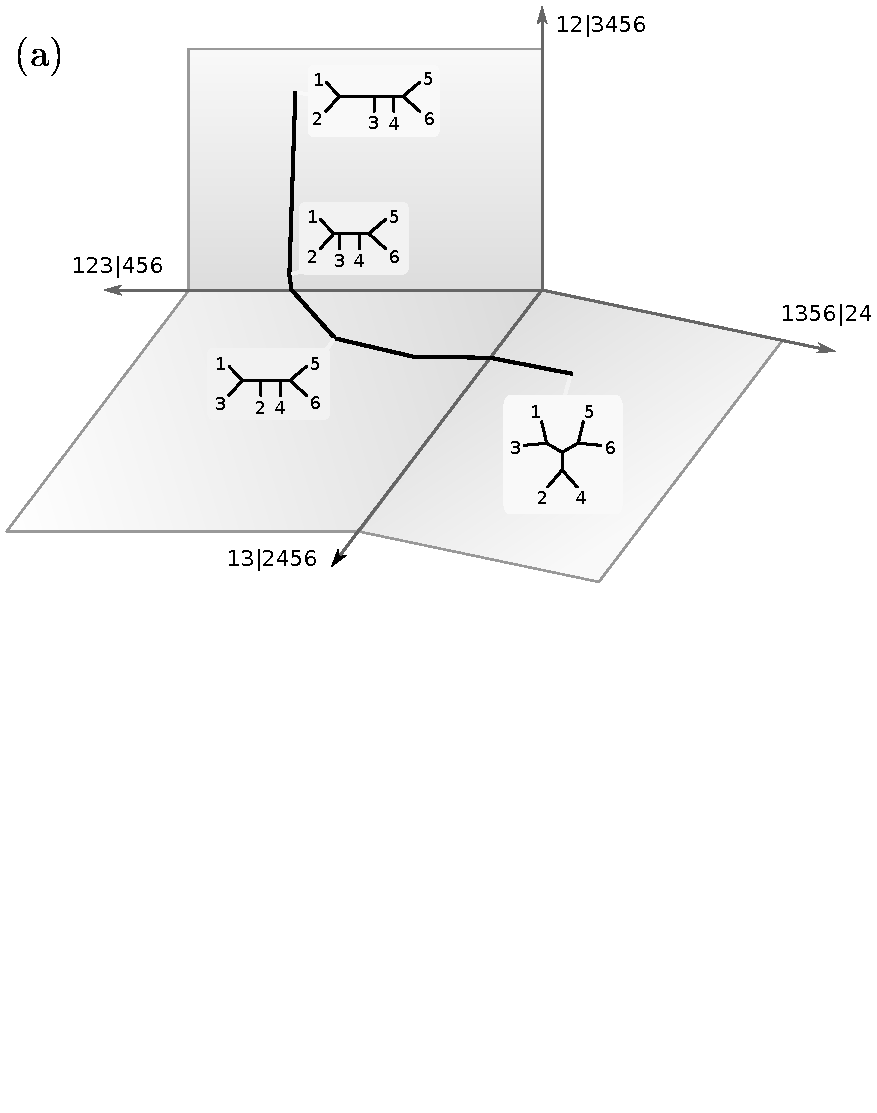
\includegraphics[height=5in]{leap-prog-a}};
      \node at (18,0) {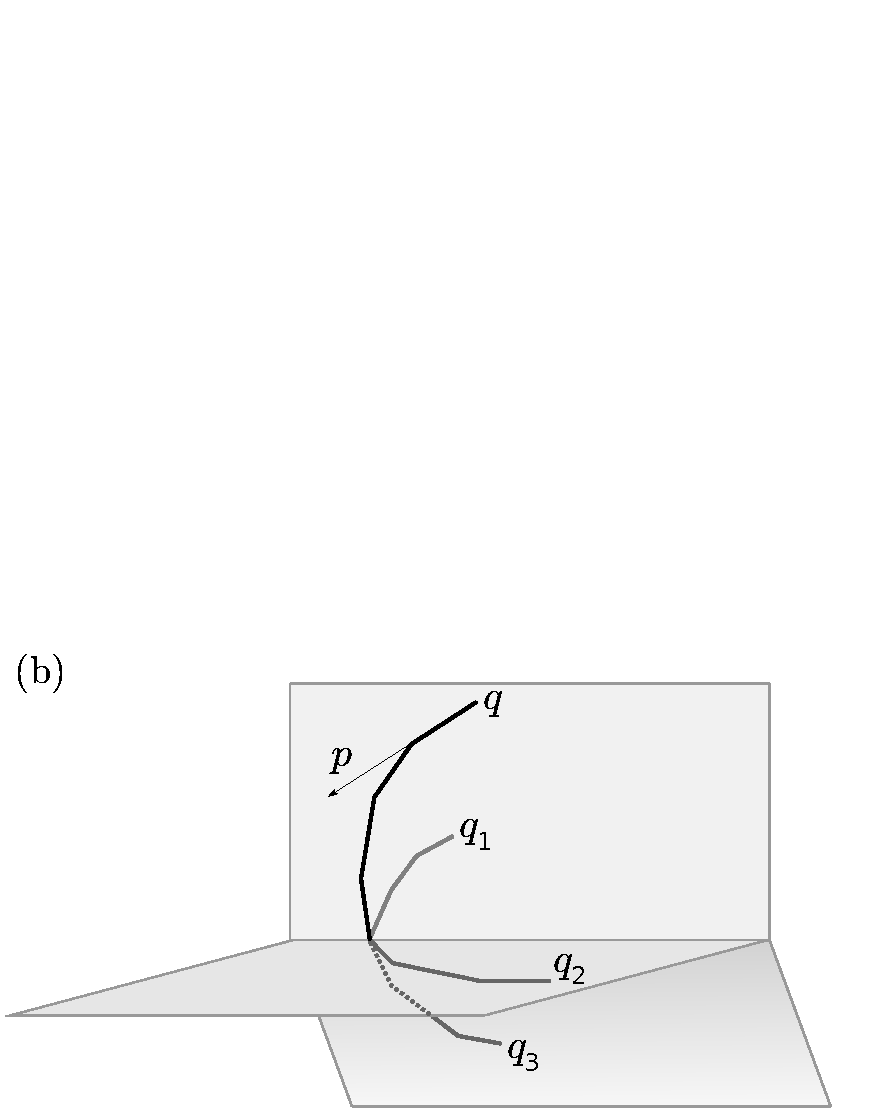
\includegraphics[height=4in]{leap-prog-b}};
    \end{tikzpicture}
  }

  \block{Probabilistic Path HMC Algorithm}{
    \begin{enumerate}
      \item \textbf{Choose random momentum} for robot from normal distribution $\vec{p} \sim \norm{\vec{0}, \mat{M}^{-1}}$
      \item Simulate its motion under smoothened surrogate $\mathcal{H}^\prime$ using \textbf{leap-prog integrator}
      \item Flip its momentum
      \item Let $a = \min\left(1, \exp\left(\mathcal{H}\left(\vec{q}, \vec{p}\right) - \mathcal{H}\left(\vec{q}^\prime, \vec{p}^\prime\right)\right)\right)$
          \begin{itemize}
              \item Remember that $\mathcal{H}$ is \textbf{approximately conserved} $\implies a \approx 1$
          \end{itemize}
      \item With probability $a$ \textbf{accept its position}; otherwise reject and put it back where it was
      \item Flip its momentum again
      \item Save its position as \textbf{sample from} $P\left(\mathcal{T}\mid D\right)$
      \item Iterate as necessary
    \end{enumerate}
  }

  \block{Results}{
    \centering
    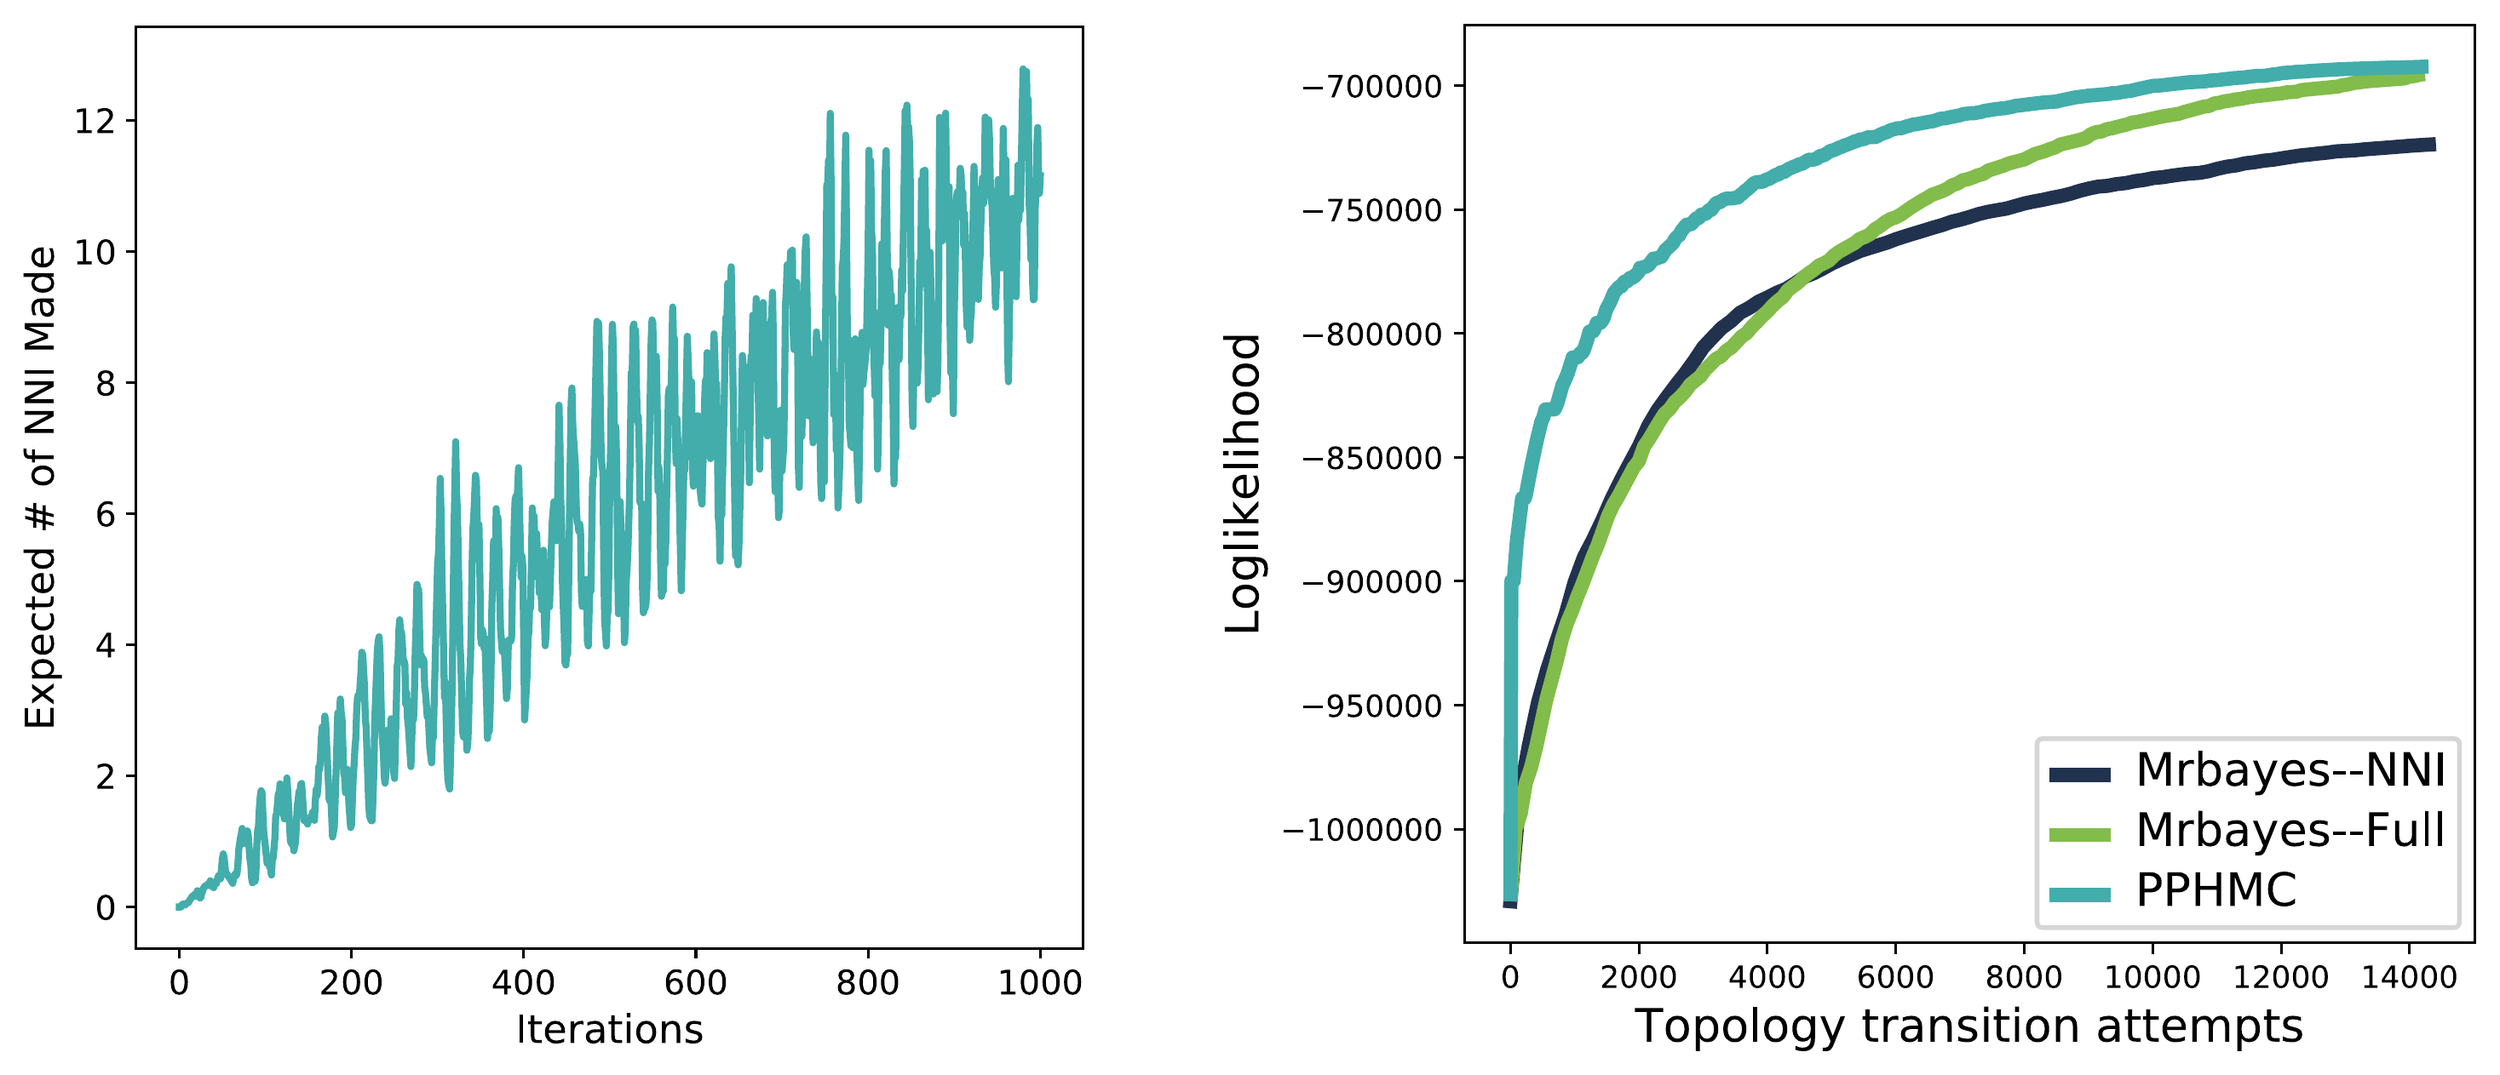
\begin{tikzpicture}
     \begin{scope}[scale=1.5,shift={(-12,1)}]
       \definecolor{cffffff}{RGB}{255,255,255}
\definecolor{c1e76b3}{RGB}{30,118,179}
\definecolor{cff7f0d}{RGB}{255,127,13}
\definecolor{ccccccc}{RGB}{204,204,204}


\begin{scope}[y=0.80pt, x=0.80pt, yscale=-1.000000, xscale=1.000000, inner sep=0pt, outer sep=0pt]
  % \path[fill=cffffff,rounded corners=0.0000cm] (0.0000,0.0000) rectangle
  %   (432.0000,432.0000);
  % \path[fill=cffffff,nonzero rule] (54.0000,378.0000) -- (388.8008,378.0000) --
  %   (388.8008,51.8398) -- (54.0000,51.8398) -- cycle(54.0000,378.0000);
  \begin{scope}[cm={{1.0,0.0,0.0,1.0,(68.0,378.0)}}]
        \path[cm={{0.1,0.0,0.0,-0.1,(-68.0,54.0)}},draw=black,line join=round,line
          cap=butt,miter limit=10.00,line width=1.1pt] (692.1875,540.0000) --
          (692.1875,505.0000);
  \end{scope}
    \path[fill=black,nonzero rule] (69.2148,386.1328) .. controls (68.6055,386.1328)
      and (68.1484,386.4336) .. (67.8359,387.0312) .. controls (67.5234,387.6328)
      and (67.3789,388.5312) .. (67.3789,389.7305) .. controls (67.3789,390.9336)
      and (67.5234,391.8320) .. (67.8359,392.4336) .. controls (68.1484,393.0312)
      and (68.6055,393.3320) .. (69.2148,393.3320) .. controls (69.8281,393.3320)
      and (70.2852,393.0312) .. (70.5977,392.4336) .. controls (70.8945,391.8320)
      and (71.0508,390.9336) .. (71.0508,389.7305) .. controls (71.0508,388.5312)
      and (70.8945,387.6328) .. (70.5977,387.0312) .. controls (70.2852,386.4336)
      and (69.8281,386.1328) .. (69.2148,386.1328)(69.2148,385.1953) .. controls
      (70.1875,385.1953) and (70.9336,385.5938) .. (71.4609,386.3594) .. controls
      (71.9766,387.1406) and (72.2383,388.2695) .. (72.2383,389.7305) .. controls
      (72.2383,391.2070) and (71.9766,392.3359) .. (71.4609,393.1055) .. controls
      (70.9336,393.8711) and (70.1875,394.2578) .. (69.2148,394.2578) .. controls
      (68.2305,394.2578) and (67.4766,393.8711) .. (66.9609,393.1055) .. controls
      (66.4453,392.3359) and (66.1914,391.2070) .. (66.1914,389.7305) .. controls
      (66.1914,388.2695) and (66.4453,387.1406) .. (66.9609,386.3594) .. controls
      (67.4766,385.5938) and (68.2305,385.1953) .. (69.2148,385.1953);
  \begin{scope}[cm={{1.0,0.0,0.0,1.0,(129.0,378.0)}}]
        \path[cm={{0.1,0.0,0.0,-0.1,(-129.0,54.0)}},draw=black,line join=round,line
          cap=butt,miter limit=10.00,line width=1.1pt] (1300.8984,540.0000) --
          (1300.8984,505.0000);
  \end{scope}
    \path[fill=black,nonzero rule] (120.9023,393.1055) -- (125.0312,393.1055) --
      (125.0312,394.1016) -- (119.4766,394.1016) -- (119.4766,393.1055) .. controls
      (119.9219,392.6484) and (120.5312,392.0234) .. (121.3125,391.2305) .. controls
      (122.0781,390.4531) and (122.5703,389.9492) .. (122.7773,389.7188) .. controls
      (123.1602,389.3008) and (123.4258,388.9414) .. (123.5664,388.6406) .. controls
      (123.7109,388.3516) and (123.7969,388.0508) .. (123.7969,387.7656) .. controls
      (123.7969,387.3086) and (123.6289,386.9219) .. (123.3047,386.6367) .. controls
      (122.9805,386.3477) and (122.5586,386.1914) .. (122.0312,386.1914) .. controls
      (121.6602,386.1914) and (121.2656,386.2656) .. (120.8555,386.3828) .. controls
      (120.4492,386.5156) and (120.0039,386.7070) .. (119.5352,386.9727) --
      (119.5352,385.7734) .. controls (120.0156,385.5820) and (120.4609,385.4375) ..
      (120.8672,385.3398) .. controls (121.2773,385.2422) and (121.6602,385.1953) ..
      (122.0078,385.1953) .. controls (122.9062,385.1953) and (123.6289,385.4219) ..
      (124.1680,385.8789) .. controls (124.7070,386.3359) and (124.9844,386.9375) ..
      (124.9844,387.6914) .. controls (124.9844,388.0508) and (124.9102,388.3984) ..
      (124.7812,388.7109) .. controls (124.6484,389.0352) and (124.4062,389.4180) ..
      (124.0469,389.8516) .. controls (123.9531,389.9727) and (123.6406,390.2969) ..
      (123.1133,390.8359) .. controls (122.5859,391.3750) and (121.8516,392.1328) ..
      (120.9023,393.1055);
    \path[fill=black,nonzero rule] (130.1172,386.1328) .. controls
      (129.5039,386.1328) and (129.0469,386.4336) .. (128.7344,387.0312) .. controls
      (128.4258,387.6328) and (128.2812,388.5312) .. (128.2812,389.7305) .. controls
      (128.2812,390.9336) and (128.4258,391.8320) .. (128.7344,392.4336) .. controls
      (129.0469,393.0312) and (129.5039,393.3320) .. (130.1172,393.3320) .. controls
      (130.7266,393.3320) and (131.1836,393.0312) .. (131.4961,392.4336) .. controls
      (131.7969,391.8320) and (131.9531,390.9336) .. (131.9531,389.7305) .. controls
      (131.9531,388.5312) and (131.7969,387.6328) .. (131.4961,387.0312) .. controls
      (131.1836,386.4336) and (130.7266,386.1328) ..
      (130.1172,386.1328)(130.1172,385.1953) .. controls (131.0898,385.1953) and
      (131.8320,385.5938) .. (132.3594,386.3594) .. controls (132.8750,387.1406) and
      (133.1406,388.2695) .. (133.1406,389.7305) .. controls (133.1406,391.2070) and
      (132.8750,392.3359) .. (132.3594,393.1055) .. controls (131.8320,393.8711) and
      (131.0898,394.2578) .. (130.1172,394.2578) .. controls (129.1328,394.2578) and
      (128.3750,393.8711) .. (127.8594,393.1055) .. controls (127.3438,392.3359) and
      (127.0938,391.2070) .. (127.0938,389.7305) .. controls (127.0938,388.2695) and
      (127.3438,387.1406) .. (127.8594,386.3594) .. controls (128.3750,385.5938) and
      (129.1328,385.1953) .. (130.1172,385.1953);
    \path[fill=black,nonzero rule] (137.7148,386.1328) .. controls
      (137.1055,386.1328) and (136.6484,386.4336) .. (136.3359,387.0312) .. controls
      (136.0234,387.6328) and (135.8789,388.5312) .. (135.8789,389.7305) .. controls
      (135.8789,390.9336) and (136.0234,391.8320) .. (136.3359,392.4336) .. controls
      (136.6484,393.0312) and (137.1055,393.3320) .. (137.7148,393.3320) .. controls
      (138.3281,393.3320) and (138.7852,393.0312) .. (139.0977,392.4336) .. controls
      (139.3945,391.8320) and (139.5508,390.9336) .. (139.5508,389.7305) .. controls
      (139.5508,388.5312) and (139.3945,387.6328) .. (139.0977,387.0312) .. controls
      (138.7852,386.4336) and (138.3281,386.1328) ..
      (137.7148,386.1328)(137.7148,385.1953) .. controls (138.6875,385.1953) and
      (139.4336,385.5938) .. (139.9609,386.3594) .. controls (140.4766,387.1406) and
      (140.7383,388.2695) .. (140.7383,389.7305) .. controls (140.7383,391.2070) and
      (140.4766,392.3359) .. (139.9609,393.1055) .. controls (139.4336,393.8711) and
      (138.6875,394.2578) .. (137.7148,394.2578) .. controls (136.7305,394.2578) and
      (135.9766,393.8711) .. (135.4609,393.1055) .. controls (134.9453,392.3359) and
      (134.6914,391.2070) .. (134.6914,389.7305) .. controls (134.6914,388.2695) and
      (134.9453,387.1406) .. (135.4609,386.3594) .. controls (135.9766,385.5938) and
      (136.7305,385.1953) .. (137.7148,385.1953);
  \begin{scope}[cm={{1.0,0.0,0.0,1.0,(190.0,378.0)}}]
        \path[cm={{0.1,0.0,0.0,-0.1,(-190.0,54.0)}},draw=black,line join=round,line
          cap=butt,miter limit=10.00,line width=1.1pt] (1909.6484,540.0000) --
          (1909.6484,505.0000);
  \end{scope}
    \path[fill=black,nonzero rule] (184.0352,386.3828) -- (181.0469,391.0508) --
      (184.0352,391.0508) -- (184.0352,386.3828)(183.7227,385.3516) --
      (185.2109,385.3516) -- (185.2109,391.0508) -- (186.4609,391.0508) --
      (186.4609,392.0352) -- (185.2109,392.0352) -- (185.2109,394.1016) --
      (184.0352,394.1016) -- (184.0352,392.0352) -- (180.0898,392.0352) --
      (180.0898,390.8945) -- (183.7227,385.3516);
    \path[fill=black,nonzero rule] (190.9141,386.1328) .. controls
      (190.3047,386.1328) and (189.8477,386.4336) .. (189.5352,387.0312) .. controls
      (189.2227,387.6328) and (189.0781,388.5312) .. (189.0781,389.7305) .. controls
      (189.0781,390.9336) and (189.2227,391.8320) .. (189.5352,392.4336) .. controls
      (189.8477,393.0312) and (190.3047,393.3320) .. (190.9141,393.3320) .. controls
      (191.5273,393.3320) and (191.9844,393.0312) .. (192.2969,392.4336) .. controls
      (192.5977,391.8320) and (192.7539,390.9336) .. (192.7539,389.7305) .. controls
      (192.7539,388.5312) and (192.5977,387.6328) .. (192.2969,387.0312) .. controls
      (191.9844,386.4336) and (191.5273,386.1328) ..
      (190.9141,386.1328)(190.9141,385.1953) .. controls (191.8867,385.1953) and
      (192.6328,385.5938) .. (193.1602,386.3594) .. controls (193.6758,387.1406) and
      (193.9414,388.2695) .. (193.9414,389.7305) .. controls (193.9414,391.2070) and
      (193.6758,392.3359) .. (193.1602,393.1055) .. controls (192.6328,393.8711) and
      (191.8867,394.2578) .. (190.9141,394.2578) .. controls (189.9336,394.2578) and
      (189.1758,393.8711) .. (188.6602,393.1055) .. controls (188.1445,392.3359) and
      (187.8906,391.2070) .. (187.8906,389.7305) .. controls (187.8906,388.2695) and
      (188.1445,387.1406) .. (188.6602,386.3594) .. controls (189.1758,385.5938) and
      (189.9336,385.1953) .. (190.9141,385.1953);
    \path[fill=black,nonzero rule] (198.6172,386.1328) .. controls
      (198.0039,386.1328) and (197.5469,386.4336) .. (197.2344,387.0312) .. controls
      (196.9258,387.6328) and (196.7812,388.5312) .. (196.7812,389.7305) .. controls
      (196.7812,390.9336) and (196.9258,391.8320) .. (197.2344,392.4336) .. controls
      (197.5469,393.0312) and (198.0039,393.3320) .. (198.6172,393.3320) .. controls
      (199.2266,393.3320) and (199.6836,393.0312) .. (199.9961,392.4336) .. controls
      (200.2969,391.8320) and (200.4531,390.9336) .. (200.4531,389.7305) .. controls
      (200.4531,388.5312) and (200.2969,387.6328) .. (199.9961,387.0312) .. controls
      (199.6836,386.4336) and (199.2266,386.1328) ..
      (198.6172,386.1328)(198.6172,385.1953) .. controls (199.5898,385.1953) and
      (200.3320,385.5938) .. (200.8594,386.3594) .. controls (201.3750,387.1406) and
      (201.6406,388.2695) .. (201.6406,389.7305) .. controls (201.6406,391.2070) and
      (201.3750,392.3359) .. (200.8594,393.1055) .. controls (200.3320,393.8711) and
      (199.5898,394.2578) .. (198.6172,394.2578) .. controls (197.6328,394.2578) and
      (196.8750,393.8711) .. (196.3594,393.1055) .. controls (195.8438,392.3359) and
      (195.5938,391.2070) .. (195.5938,389.7305) .. controls (195.5938,388.2695) and
      (195.8438,387.1406) .. (196.3594,386.3594) .. controls (196.8750,385.5938) and
      (197.6328,385.1953) .. (198.6172,385.1953);
  \begin{scope}[cm={{1.0,0.0,0.0,1.0,(251.0,378.0)}}]
        \path[cm={{0.1,0.0,0.0,-0.1,(-251.0,54.0)}},draw=black,line join=round,line
          cap=butt,miter limit=10.00,line width=1.1pt] (2518.3594,540.0000) --
          (2518.3594,505.0000);
  \end{scope}
    \path[fill=black,nonzero rule] (244.3594,389.2539) .. controls
      (243.8320,389.2539) and (243.4102,389.4453) .. (243.1016,389.8047) .. controls
      (242.7891,390.1641) and (242.6328,390.6680) .. (242.6328,391.2930) .. controls
      (242.6328,391.9297) and (242.7891,392.4336) .. (243.1016,392.7930) .. controls
      (243.4102,393.1523) and (243.8320,393.3320) .. (244.3594,393.3320) .. controls
      (244.8867,393.3320) and (245.3086,393.1523) .. (245.6211,392.7930) .. controls
      (245.9336,392.4336) and (246.0898,391.9297) .. (246.0898,391.2930) .. controls
      (246.0898,390.6680) and (245.9336,390.1641) .. (245.6211,389.8047) .. controls
      (245.3086,389.4453) and (244.8867,389.2539) ..
      (244.3594,389.2539)(246.7109,385.5430) -- (246.7109,386.6250) .. controls
      (246.4102,386.4805) and (246.1133,386.3711) .. (245.8125,386.3008) .. controls
      (245.5000,386.2266) and (245.1992,386.1914) .. (244.9102,386.1914) .. controls
      (244.1211,386.1914) and (243.5195,386.4570) .. (243.1133,386.9844) .. controls
      (242.7031,387.5117) and (242.4648,388.3164) .. (242.4141,389.3711) .. controls
      (242.6445,389.0352) and (242.9336,388.7734) .. (243.2812,388.5938) .. controls
      (243.6289,388.4102) and (244.0117,388.3164) .. (244.4336,388.3164) .. controls
      (245.3086,388.3164) and (246.0039,388.5938) .. (246.5078,389.1211) .. controls
      (247.0117,389.6484) and (247.2773,390.3789) .. (247.2773,391.2930) .. controls
      (247.2773,392.1914) and (247.0000,392.9102) .. (246.4727,393.4531) .. controls
      (245.9453,393.9922) and (245.2344,394.2578) .. (244.3594,394.2578) .. controls
      (243.3516,394.2578) and (242.5703,393.8711) .. (242.0430,393.1055) .. controls
      (241.5039,392.3359) and (241.2383,391.2070) .. (241.2383,389.7305) .. controls
      (241.2383,388.3516) and (241.5625,387.2461) .. (242.2227,386.4336) .. controls
      (242.8711,385.6172) and (243.7617,385.1953) .. (244.8633,385.1953) .. controls
      (245.1523,385.1953) and (245.4531,385.2305) .. (245.7656,385.2812) .. controls
      (246.0625,385.3398) and (246.3750,385.4219) .. (246.7109,385.5430);
    \path[fill=black,nonzero rule] (251.8164,386.1328) .. controls
      (251.2031,386.1328) and (250.7461,386.4336) .. (250.4375,387.0312) .. controls
      (250.1250,387.6328) and (249.9805,388.5312) .. (249.9805,389.7305) .. controls
      (249.9805,390.9336) and (250.1250,391.8320) .. (250.4375,392.4336) .. controls
      (250.7461,393.0312) and (251.2031,393.3320) .. (251.8164,393.3320) .. controls
      (252.4297,393.3320) and (252.8828,393.0312) .. (253.1953,392.4336) .. controls
      (253.4961,391.8320) and (253.6523,390.9336) .. (253.6523,389.7305) .. controls
      (253.6523,388.5312) and (253.4961,387.6328) .. (253.1953,387.0312) .. controls
      (252.8828,386.4336) and (252.4297,386.1328) ..
      (251.8164,386.1328)(251.8164,385.1953) .. controls (252.7891,385.1953) and
      (253.5312,385.5938) .. (254.0586,386.3594) .. controls (254.5742,387.1406) and
      (254.8398,388.2695) .. (254.8398,389.7305) .. controls (254.8398,391.2070) and
      (254.5742,392.3359) .. (254.0586,393.1055) .. controls (253.5312,393.8711) and
      (252.7891,394.2578) .. (251.8164,394.2578) .. controls (250.8320,394.2578) and
      (250.0742,393.8711) .. (249.5586,393.1055) .. controls (249.0430,392.3359) and
      (248.7930,391.2070) .. (248.7930,389.7305) .. controls (248.7930,388.2695) and
      (249.0430,387.1406) .. (249.5586,386.3594) .. controls (250.0742,385.5938) and
      (250.8320,385.1953) .. (251.8164,385.1953);
    \path[fill=black,nonzero rule] (259.4141,386.1328) .. controls
      (258.8047,386.1328) and (258.3477,386.4336) .. (258.0352,387.0312) .. controls
      (257.7227,387.6328) and (257.5781,388.5312) .. (257.5781,389.7305) .. controls
      (257.5781,390.9336) and (257.7227,391.8320) .. (258.0352,392.4336) .. controls
      (258.3477,393.0312) and (258.8047,393.3320) .. (259.4141,393.3320) .. controls
      (260.0273,393.3320) and (260.4844,393.0312) .. (260.7969,392.4336) .. controls
      (261.0977,391.8320) and (261.2539,390.9336) .. (261.2539,389.7305) .. controls
      (261.2539,388.5312) and (261.0977,387.6328) .. (260.7969,387.0312) .. controls
      (260.4844,386.4336) and (260.0273,386.1328) ..
      (259.4141,386.1328)(259.4141,385.1953) .. controls (260.3867,385.1953) and
      (261.1328,385.5938) .. (261.6602,386.3594) .. controls (262.1758,387.1406) and
      (262.4414,388.2695) .. (262.4414,389.7305) .. controls (262.4414,391.2070) and
      (262.1758,392.3359) .. (261.6602,393.1055) .. controls (261.1328,393.8711) and
      (260.3867,394.2578) .. (259.4141,394.2578) .. controls (258.4336,394.2578) and
      (257.6758,393.8711) .. (257.1602,393.1055) .. controls (256.6445,392.3359) and
      (256.3906,391.2070) .. (256.3906,389.7305) .. controls (256.3906,388.2695) and
      (256.6445,387.1406) .. (257.1602,386.3594) .. controls (257.6758,385.5938) and
      (258.4336,385.1953) .. (259.4141,385.1953);
  \begin{scope}[cm={{1.0,0.0,0.0,1.0,(312.0,378.0)}}]
        \path[cm={{0.1,0.0,0.0,-0.1,(-312.0,54.0)}},draw=black,line join=round,line
          cap=butt,miter limit=10.00,line width=1.1pt] (3127.1094,540.0000) --
          (3127.1094,505.0000);
  \end{scope}
    \path[fill=black,nonzero rule] (305.0156,389.9492) .. controls
      (304.4531,389.9492) and (304.0078,390.1055) .. (303.6836,390.4023) .. controls
      (303.3594,390.7031) and (303.2031,391.1133) .. (303.2031,391.6406) .. controls
      (303.2031,392.1680) and (303.3594,392.5898) .. (303.6836,392.8867) .. controls
      (304.0078,393.1875) and (304.4531,393.3320) .. (305.0156,393.3320) .. controls
      (305.5664,393.3320) and (306.0117,393.1875) .. (306.3359,392.8750) .. controls
      (306.6602,392.5781) and (306.8281,392.1680) .. (306.8281,391.6406) .. controls
      (306.8281,391.1133) and (306.6602,390.7031) .. (306.3477,390.4023) .. controls
      (306.0234,390.1055) and (305.5781,389.9492) ..
      (305.0156,389.9492)(303.8281,389.4453) .. controls (303.3242,389.3242) and
      (302.9297,389.0859) .. (302.6406,388.7344) .. controls (302.3516,388.3867) and
      (302.2188,387.9688) .. (302.2188,387.4648) .. controls (302.2188,386.7695) and
      (302.4609,386.2148) .. (302.9648,385.8086) .. controls (303.4570,385.3984) and
      (304.1406,385.1953) .. (305.0156,385.1953) .. controls (305.8789,385.1953) and
      (306.5625,385.3984) .. (307.0664,385.8086) .. controls (307.5586,386.2148) and
      (307.8125,386.7695) .. (307.8125,387.4648) .. controls (307.8125,387.9688) and
      (307.6680,388.3867) .. (307.3789,388.7344) .. controls (307.0938,389.0859) and
      (306.7070,389.3242) .. (306.2031,389.4453) .. controls (306.7695,389.5781) and
      (307.2109,389.8398) .. (307.5352,390.2227) .. controls (307.8477,390.6094) and
      (308.0156,391.0898) .. (308.0156,391.6406) .. controls (308.0156,392.4922) and
      (307.7539,393.1406) .. (307.2344,393.5859) .. controls (306.7070,394.0391) and
      (305.9766,394.2578) .. (305.0156,394.2578) .. controls (304.0430,394.2578) and
      (303.3008,394.0391) .. (302.7852,393.5859) .. controls (302.2695,393.1406) and
      (302.0156,392.4922) .. (302.0156,391.6406) .. controls (302.0156,391.0898) and
      (302.1719,390.6094) .. (302.4961,390.2227) .. controls (302.8086,389.8398) and
      (303.2539,389.5781) .. (303.8281,389.4453)(303.3945,387.5703) .. controls
      (303.3945,388.0273) and (303.5273,388.3867) .. (303.8164,388.6406) .. controls
      (304.1055,388.8906) and (304.5000,389.0117) .. (305.0156,389.0117) .. controls
      (305.5195,389.0117) and (305.9141,388.8906) .. (306.2031,388.6406) .. controls
      (306.4922,388.3867) and (306.6367,388.0273) .. (306.6367,387.5703) .. controls
      (306.6367,387.1172) and (306.4922,386.7695) .. (306.2031,386.5156) .. controls
      (305.9141,386.2656) and (305.5195,386.1328) .. (305.0156,386.1328) .. controls
      (304.5000,386.1328) and (304.1055,386.2656) .. (303.8164,386.5156) .. controls
      (303.5273,386.7695) and (303.3945,387.1172) .. (303.3945,387.5703);
    \path[fill=black,nonzero rule] (312.7148,386.1328) .. controls
      (312.1055,386.1328) and (311.6484,386.4336) .. (311.3359,387.0312) .. controls
      (311.0234,387.6328) and (310.8789,388.5312) .. (310.8789,389.7305) .. controls
      (310.8789,390.9336) and (311.0234,391.8320) .. (311.3359,392.4336) .. controls
      (311.6484,393.0312) and (312.1055,393.3320) .. (312.7148,393.3320) .. controls
      (313.3281,393.3320) and (313.7852,393.0312) .. (314.0977,392.4336) .. controls
      (314.3945,391.8320) and (314.5508,390.9336) .. (314.5508,389.7305) .. controls
      (314.5508,388.5312) and (314.3945,387.6328) .. (314.0977,387.0312) .. controls
      (313.7852,386.4336) and (313.3281,386.1328) ..
      (312.7148,386.1328)(312.7148,385.1953) .. controls (313.6875,385.1953) and
      (314.4336,385.5938) .. (314.9609,386.3594) .. controls (315.4766,387.1406) and
      (315.7383,388.2695) .. (315.7383,389.7305) .. controls (315.7383,391.2070) and
      (315.4766,392.3359) .. (314.9609,393.1055) .. controls (314.4336,393.8711) and
      (313.6875,394.2578) .. (312.7148,394.2578) .. controls (311.7305,394.2578) and
      (310.9766,393.8711) .. (310.4609,393.1055) .. controls (309.9453,392.3359) and
      (309.6914,391.2070) .. (309.6914,389.7305) .. controls (309.6914,388.2695) and
      (309.9453,387.1406) .. (310.4609,386.3594) .. controls (310.9766,385.5938) and
      (311.7305,385.1953) .. (312.7148,385.1953);
    \path[fill=black,nonzero rule] (320.3164,386.1328) .. controls
      (319.7031,386.1328) and (319.2461,386.4336) .. (318.9375,387.0312) .. controls
      (318.6250,387.6328) and (318.4805,388.5312) .. (318.4805,389.7305) .. controls
      (318.4805,390.9336) and (318.6250,391.8320) .. (318.9375,392.4336) .. controls
      (319.2461,393.0312) and (319.7031,393.3320) .. (320.3164,393.3320) .. controls
      (320.9297,393.3320) and (321.3828,393.0312) .. (321.6953,392.4336) .. controls
      (321.9961,391.8320) and (322.1523,390.9336) .. (322.1523,389.7305) .. controls
      (322.1523,388.5312) and (321.9961,387.6328) .. (321.6953,387.0312) .. controls
      (321.3828,386.4336) and (320.9297,386.1328) ..
      (320.3164,386.1328)(320.3164,385.1953) .. controls (321.2891,385.1953) and
      (322.0312,385.5938) .. (322.5586,386.3594) .. controls (323.0742,387.1406) and
      (323.3398,388.2695) .. (323.3398,389.7305) .. controls (323.3398,391.2070) and
      (323.0742,392.3359) .. (322.5586,393.1055) .. controls (322.0312,393.8711) and
      (321.2891,394.2578) .. (320.3164,394.2578) .. controls (319.3320,394.2578) and
      (318.5742,393.8711) .. (318.0586,393.1055) .. controls (317.5430,392.3359) and
      (317.2930,391.2070) .. (317.2930,389.7305) .. controls (317.2930,388.2695) and
      (317.5430,387.1406) .. (318.0586,386.3594) .. controls (318.5742,385.5938) and
      (319.3320,385.1953) .. (320.3164,385.1953);
  \begin{scope}[cm={{1.0,0.0,0.0,1.0,(373.0,378.0)}}]
        \path[cm={{0.1,0.0,0.0,-0.1,(-373.0,54.0)}},draw=black,line join=round,line
          cap=butt,miter limit=10.00,line width=1.1pt] (3735.8203,540.0000) --
          (3735.8203,505.0000);
  \end{scope}
    \path[fill=black,nonzero rule] (359.7891,393.1055) -- (361.7188,393.1055) --
      (361.7188,386.4336) -- (359.6211,386.8516) -- (359.6211,385.7734) --
      (361.7070,385.3516) -- (362.8945,385.3516) -- (362.8945,393.1055) --
      (364.8281,393.1055) -- (364.8281,394.1016) -- (359.7891,394.1016) --
      (359.7891,393.1055);
    \path[fill=black,nonzero rule] (369.7148,386.1328) .. controls
      (369.1055,386.1328) and (368.6484,386.4336) .. (368.3359,387.0312) .. controls
      (368.0234,387.6328) and (367.8789,388.5312) .. (367.8789,389.7305) .. controls
      (367.8789,390.9336) and (368.0234,391.8320) .. (368.3359,392.4336) .. controls
      (368.6484,393.0312) and (369.1055,393.3320) .. (369.7148,393.3320) .. controls
      (370.3281,393.3320) and (370.7852,393.0312) .. (371.0977,392.4336) .. controls
      (371.3945,391.8320) and (371.5508,390.9336) .. (371.5508,389.7305) .. controls
      (371.5508,388.5312) and (371.3945,387.6328) .. (371.0977,387.0312) .. controls
      (370.7852,386.4336) and (370.3281,386.1328) ..
      (369.7148,386.1328)(369.7148,385.1953) .. controls (370.6875,385.1953) and
      (371.4336,385.5938) .. (371.9609,386.3594) .. controls (372.4766,387.1406) and
      (372.7383,388.2695) .. (372.7383,389.7305) .. controls (372.7383,391.2070) and
      (372.4766,392.3359) .. (371.9609,393.1055) .. controls (371.4336,393.8711) and
      (370.6875,394.2578) .. (369.7148,394.2578) .. controls (368.7305,394.2578) and
      (367.9766,393.8711) .. (367.4609,393.1055) .. controls (366.9453,392.3359) and
      (366.6914,391.2070) .. (366.6914,389.7305) .. controls (366.6914,388.2695) and
      (366.9453,387.1406) .. (367.4609,386.3594) .. controls (367.9766,385.5938) and
      (368.7305,385.1953) .. (369.7148,385.1953);
    \path[fill=black,nonzero rule] (377.4141,386.1328) .. controls
      (376.8047,386.1328) and (376.3477,386.4336) .. (376.0352,387.0312) .. controls
      (375.7227,387.6328) and (375.5781,388.5312) .. (375.5781,389.7305) .. controls
      (375.5781,390.9336) and (375.7227,391.8320) .. (376.0352,392.4336) .. controls
      (376.3477,393.0312) and (376.8047,393.3320) .. (377.4141,393.3320) .. controls
      (378.0273,393.3320) and (378.4844,393.0312) .. (378.7969,392.4336) .. controls
      (379.0977,391.8320) and (379.2539,390.9336) .. (379.2539,389.7305) .. controls
      (379.2539,388.5312) and (379.0977,387.6328) .. (378.7969,387.0312) .. controls
      (378.4844,386.4336) and (378.0273,386.1328) ..
      (377.4141,386.1328)(377.4141,385.1953) .. controls (378.3867,385.1953) and
      (379.1328,385.5938) .. (379.6602,386.3594) .. controls (380.1758,387.1406) and
      (380.4414,388.2695) .. (380.4414,389.7305) .. controls (380.4414,391.2070) and
      (380.1758,392.3359) .. (379.6602,393.1055) .. controls (379.1328,393.8711) and
      (378.3867,394.2578) .. (377.4141,394.2578) .. controls (376.4336,394.2578) and
      (375.6758,393.8711) .. (375.1602,393.1055) .. controls (374.6445,392.3359) and
      (374.3906,391.2070) .. (374.3906,389.7305) .. controls (374.3906,388.2695) and
      (374.6445,387.1406) .. (375.1602,386.3594) .. controls (375.6758,385.5938) and
      (376.4336,385.1953) .. (377.4141,385.1953);
    \path[fill=black,nonzero rule] (385.0156,386.1328) .. controls
      (384.4023,386.1328) and (383.9492,386.4336) .. (383.6367,387.0312) .. controls
      (383.3242,387.6328) and (383.1797,388.5312) .. (383.1797,389.7305) .. controls
      (383.1797,390.9336) and (383.3242,391.8320) .. (383.6367,392.4336) .. controls
      (383.9492,393.0312) and (384.4023,393.3320) .. (385.0156,393.3320) .. controls
      (385.6289,393.3320) and (386.0859,393.0312) .. (386.3945,392.4336) .. controls
      (386.6953,391.8320) and (386.8516,390.9336) .. (386.8516,389.7305) .. controls
      (386.8516,388.5312) and (386.6953,387.6328) .. (386.3945,387.0312) .. controls
      (386.0859,386.4336) and (385.6289,386.1328) ..
      (385.0156,386.1328)(385.0156,385.1953) .. controls (385.9883,385.1953) and
      (386.7305,385.5938) .. (387.2617,386.3594) .. controls (387.7773,387.1406) and
      (388.0391,388.2695) .. (388.0391,389.7305) .. controls (388.0391,391.2070) and
      (387.7773,392.3359) .. (387.2617,393.1055) .. controls (386.7305,393.8711) and
      (385.9883,394.2578) .. (385.0156,394.2578) .. controls (384.0312,394.2578) and
      (383.2773,393.8711) .. (382.7617,393.1055) .. controls (382.2422,392.3359) and
      (381.9922,391.2070) .. (381.9922,389.7305) .. controls (381.9922,388.2695) and
      (382.2422,387.1406) .. (382.7617,386.3594) .. controls (383.2773,385.5938) and
      (384.0312,385.1953) .. (385.0156,385.1953);
    \path[fill=black,nonzero rule] (189.4727,411.3008) -- (190.8594,411.3008) --
      (190.8594,401.0938) -- (189.4727,401.0938) -- cycle(189.4727,411.3008);
    \path[fill=black,nonzero rule] (194.7617,401.4727) -- (194.7617,403.6406) --
      (197.3516,403.6406) -- (197.3516,404.6211) -- (194.7617,404.6211) --
      (194.7617,408.7812) .. controls (194.7617,409.4102) and (194.8477,409.8164) ..
      (195.0156,409.9844) .. controls (195.1836,410.1641) and (195.5312,410.2500) ..
      (196.0625,410.2500) -- (197.3516,410.2500) -- (197.3516,411.3008) --
      (196.0625,411.3008) .. controls (195.0859,411.3008) and (194.4102,411.1172) ..
      (194.0469,410.7539) .. controls (193.6836,410.3906) and (193.5039,409.7305) ..
      (193.5039,408.7812) -- (193.5039,404.6211) -- (192.5781,404.6211) --
      (192.5781,403.6406) -- (193.5039,403.6406) -- (193.5039,401.4727) --
      (194.7617,401.4727);
    \path[fill=black,nonzero rule] (205.5664,407.1562) -- (205.5664,407.7734) --
      (199.7852,407.7734) .. controls (199.8438,408.6406) and (200.0938,409.3125) ..
      (200.5703,409.7617) .. controls (201.0312,410.2070) and (201.6758,410.4336) ..
      (202.5156,410.4336) .. controls (202.9922,410.4336) and (203.4688,410.3750) ..
      (203.9141,410.2656) .. controls (204.3633,410.1523) and (204.8242,409.9688) ..
      (205.2734,409.7188) -- (205.2734,410.9062) .. controls (204.8242,411.1055) and
      (204.3633,411.2578) .. (203.8867,411.3438) .. controls (203.4102,411.4258) and
      (202.9219,411.4805) .. (202.4453,411.4805) .. controls (201.2148,411.4805) and
      (200.2461,411.1328) .. (199.5352,410.4336) .. controls (198.8203,409.7305) and
      (198.4688,408.7656) .. (198.4688,407.5469) .. controls (198.4688,406.3008) and
      (198.8047,405.3086) .. (199.4766,404.5664) .. controls (200.1484,403.8398) and
      (201.0742,403.4609) .. (202.2227,403.4609) .. controls (203.2578,403.4609) and
      (204.0703,403.7969) .. (204.6719,404.4531) .. controls (205.2617,405.1250) and
      (205.5664,406.0234) .. (205.5664,407.1562)(204.3086,406.7930) .. controls
      (204.2930,406.1055) and (204.0977,405.5586) .. (203.7344,405.1406) .. controls
      (203.3555,404.7344) and (202.8516,404.5234) .. (202.2344,404.5234) .. controls
      (201.5352,404.5234) and (200.9766,404.7344) .. (200.5547,405.1250) .. controls
      (200.1367,405.5195) and (199.8828,406.0781) .. (199.8281,406.7930) --
      (204.3086,406.7930);
    \path[fill=black,nonzero rule] (212.0547,404.8164) .. controls
      (211.9141,404.7344) and (211.7617,404.6797) .. (211.5938,404.6367) .. controls
      (211.4258,404.6094) and (211.2422,404.5820) .. (211.0469,404.5820) .. controls
      (210.3320,404.5820) and (209.7852,404.8164) .. (209.4062,405.2812) .. controls
      (209.0156,405.7422) and (208.8359,406.3984) .. (208.8359,407.2695) --
      (208.8359,411.3008) -- (207.5742,411.3008) -- (207.5742,403.6406) --
      (208.8359,403.6406) -- (208.8359,404.8320) .. controls (209.0859,404.3711) and
      (209.4375,404.0195) .. (209.8555,403.7969) .. controls (210.2773,403.5703) and
      (210.7930,403.4609) .. (211.4102,403.4609) .. controls (211.4922,403.4609) and
      (211.5938,403.4727) .. (211.7031,403.4727) .. controls (211.8008,403.4883) and
      (211.9141,403.5039) .. (212.0547,403.5312) -- (212.0547,404.8164);
    \path[fill=black,nonzero rule] (216.9023,407.4492) .. controls
      (215.8789,407.4492) and (215.1797,407.5781) .. (214.7891,407.8008) .. controls
      (214.3945,408.0391) and (214.1992,408.4297) .. (214.1992,408.9883) .. controls
      (214.1992,409.4375) and (214.3398,409.8008) .. (214.6328,410.0547) .. controls
      (214.9297,410.3203) and (215.3359,410.4453) .. (215.8398,410.4453) .. controls
      (216.5391,410.4453) and (217.0977,410.2070) .. (217.5195,409.7031) .. controls
      (217.9375,409.2148) and (218.1484,408.5547) .. (218.1484,407.7305) --
      (218.1484,407.4492) -- (216.9023,407.4492)(219.4062,406.9336) --
      (219.4062,411.3008) -- (218.1484,411.3008) -- (218.1484,410.1367) .. controls
      (217.8555,410.6133) and (217.4883,410.9492) .. (217.0703,411.1602) .. controls
      (216.6484,411.3711) and (216.1172,411.4805) .. (215.5039,411.4805) .. controls
      (214.7188,411.4805) and (214.0898,411.2734) .. (213.6250,410.8398) .. controls
      (213.1641,410.4023) and (212.9414,409.8164) .. (212.9414,409.0742) .. controls
      (212.9414,408.2188) and (213.2188,407.5781) .. (213.8086,407.1289) .. controls
      (214.3828,406.6953) and (215.2344,406.4688) .. (216.3828,406.4688) --
      (218.1484,406.4688) -- (218.1484,406.3438) .. controls (218.1484,405.7695) and
      (217.9531,405.3203) .. (217.5742,405.0000) .. controls (217.1953,404.6914) and
      (216.6641,404.5234) .. (215.9766,404.5234) .. controls (215.5312,404.5234) and
      (215.1094,404.5820) .. (214.6914,404.6914) .. controls (214.2695,404.8047) and
      (213.8789,404.9570) .. (213.5000,405.1523) -- (213.5000,403.9922) .. controls
      (213.9492,403.8242) and (214.3945,403.6836) .. (214.8281,403.6016) .. controls
      (215.2656,403.5156) and (215.6836,403.4609) .. (216.1055,403.4609) .. controls
      (217.2109,403.4609) and (218.0352,403.7539) .. (218.5820,404.3281) .. controls
      (219.1289,404.9023) and (219.4062,405.7695) .. (219.4062,406.9336);
    \path[fill=black,nonzero rule] (223.1602,401.4727) -- (223.1602,403.6406) --
      (225.7539,403.6406) -- (225.7539,404.6211) -- (223.1602,404.6211) --
      (223.1602,408.7812) .. controls (223.1602,409.4102) and (223.2461,409.8164) ..
      (223.4141,409.9844) .. controls (223.5820,410.1641) and (223.9336,410.2500) ..
      (224.4648,410.2500) -- (225.7539,410.2500) -- (225.7539,411.3008) --
      (224.4648,411.3008) .. controls (223.4844,411.3008) and (222.8125,411.1172) ..
      (222.4492,410.7539) .. controls (222.0859,410.3906) and (221.9023,409.7305) ..
      (221.9023,408.7812) -- (221.9023,404.6211) -- (220.9766,404.6211) --
      (220.9766,403.6406) -- (221.9023,403.6406) -- (221.9023,401.4727) --
      (223.1602,401.4727);
    \path[fill=black,nonzero rule] (227.4141,403.6406) -- (228.6758,403.6406) --
      (228.6758,411.3008) -- (227.4141,411.3008) --
      (227.4141,403.6406)(227.4141,400.6602) -- (228.6758,400.6602) --
      (228.6758,402.2578) -- (227.4141,402.2578) -- (227.4141,400.6602);
    \path[fill=black,nonzero rule] (234.2852,404.5234) .. controls
      (233.6133,404.5234) and (233.0781,404.7891) .. (232.6875,405.3203) .. controls
      (232.2969,405.8555) and (232.1016,406.5664) .. (232.1016,407.4766) .. controls
      (232.1016,408.4023) and (232.2812,409.1172) .. (232.6758,409.6484) .. controls
      (233.0664,410.1797) and (233.5977,410.4336) .. (234.2852,410.4336) .. controls
      (234.9570,410.4336) and (235.4883,410.1797) .. (235.8789,409.6484) .. controls
      (236.2734,409.1172) and (236.4688,408.4023) .. (236.4688,407.4766) .. controls
      (236.4688,406.5820) and (236.2734,405.8555) .. (235.8789,405.3203) .. controls
      (235.4883,404.7891) and (234.9570,404.5234) ..
      (234.2852,404.5234)(234.2852,403.4609) .. controls (235.3750,403.4609) and
      (236.2305,403.8242) .. (236.8594,404.5234) .. controls (237.4766,405.2383) and
      (237.7969,406.2188) .. (237.7969,407.4766) .. controls (237.7969,408.7383) and
      (237.4766,409.7188) .. (236.8594,410.4180) .. controls (236.2305,411.1328) and
      (235.3750,411.4805) .. (234.2852,411.4805) .. controls (233.1797,411.4805) and
      (232.3086,411.1328) .. (231.6953,410.4180) .. controls (231.0781,409.7188) and
      (230.7695,408.7383) .. (230.7695,407.4766) .. controls (230.7695,406.2188) and
      (231.0781,405.2383) .. (231.6953,404.5234) .. controls (232.3086,403.8242) and
      (233.1797,403.4609) .. (234.2852,403.4609);
    \path[fill=black,nonzero rule] (246.2852,406.6797) -- (246.2852,411.3008) --
      (245.0273,411.3008) -- (245.0273,406.7227) .. controls (245.0273,405.9922) and
      (244.8711,405.4609) .. (244.5938,405.0977) .. controls (244.3125,404.7344) and
      (243.8906,404.5508) .. (243.3320,404.5508) .. controls (242.6445,404.5508) and
      (242.1133,404.7773) .. (241.7227,405.2109) .. controls (241.3281,405.6445) and
      (241.1328,406.2305) .. (241.1328,406.9727) -- (241.1328,411.3008) --
      (239.8750,411.3008) -- (239.8750,403.6406) -- (241.1328,403.6406) --
      (241.1328,404.8320) .. controls (241.4297,404.3828) and (241.7773,404.0352) ..
      (242.1992,403.8086) .. controls (242.6055,403.5859) and (243.0781,403.4609) ..
      (243.6133,403.4609) .. controls (244.4805,403.4609) and (245.1523,403.7383) ..
      (245.6016,404.2852) .. controls (246.0469,404.8320) and (246.2852,405.6289) ..
      (246.2852,406.6797);
    \path[fill=black,nonzero rule] (253.7031,403.8672) -- (253.7031,405.0547) ..
      controls (253.3398,404.8867) and (252.9727,404.7461) .. (252.5977,404.6484) ..
      controls (252.2031,404.5664) and (251.8125,404.5117) .. (251.4062,404.5117) ..
      controls (250.7773,404.5117) and (250.3008,404.6094) .. (249.9922,404.8047) ..
      controls (249.6836,405.0000) and (249.5312,405.2812) .. (249.5312,405.6562) ..
      controls (249.5312,405.9531) and (249.6406,406.1758) .. (249.8672,406.3438) ..
      controls (250.0898,406.5117) and (250.5391,406.6797) .. (251.2109,406.8203) --
      (251.6445,406.9180) .. controls (252.5391,407.1133) and (253.1719,407.3945) ..
      (253.5469,407.7305) .. controls (253.9102,408.0820) and (254.1094,408.5703) ..
      (254.1094,409.1875) .. controls (254.1094,409.8984) and (253.8281,410.4609) ..
      (253.2695,410.8672) .. controls (252.7070,411.2852) and (251.9258,411.4805) ..
      (250.9453,411.4805) .. controls (250.5234,411.4805) and (250.1055,411.4414) ..
      (249.6562,411.3711) .. controls (249.2070,411.3008) and (248.7461,411.1875) ..
      (248.2578,411.0195) -- (248.2578,409.7188) .. controls (248.7188,409.9688) and
      (249.1797,410.1523) .. (249.6289,410.2656) .. controls (250.0742,410.3906) and
      (250.5234,410.4453) .. (250.9727,410.4453) .. controls (251.5586,410.4453) and
      (252.0234,410.3477) .. (252.3438,410.1523) .. controls (252.6523,409.9570) and
      (252.8203,409.6602) .. (252.8203,409.2852) .. controls (252.8203,408.9492) and
      (252.6953,408.6836) .. (252.4688,408.5000) .. controls (252.2461,408.3164) and
      (251.7422,408.1367) .. (250.9570,407.9688) -- (250.5234,407.8711) .. controls
      (249.7383,407.7031) and (249.1641,407.4492) .. (248.8281,407.1133) .. controls
      (248.4805,406.7773) and (248.3125,406.3164) .. (248.3125,405.7148) .. controls
      (248.3125,405.0000) and (248.5625,404.4414) .. (249.0664,404.0469) .. controls
      (249.5703,403.6562) and (250.3008,403.4609) .. (251.2539,403.4609) .. controls
      (251.7148,403.4609) and (252.1484,403.5039) .. (252.5664,403.5703) .. controls
      (252.9727,403.6406) and (253.3516,403.7383) .. (253.7031,403.8672);
  \begin{scope}[cm={{1.0,0.0,0.0,1.0,(50.0,362.0)}}]
        \path[cm={{0.1,0.0,0.0,-0.1,(-50.0,70.0)}},draw=black,line join=round,line
          cap=butt,miter limit=10.00,line width=1.1pt] (540.0000,688.2422) --
          (505.0000,688.2422);
  \end{scope}
    \path[fill=black,nonzero rule] (43.2148,359.7305) .. controls (42.6055,359.7305)
      and (42.1484,360.0312) .. (41.8359,360.6328) .. controls (41.5234,361.2305)
      and (41.3789,362.1328) .. (41.3789,363.3320) .. controls (41.3789,364.5312)
      and (41.5234,365.4336) .. (41.8359,366.0312) .. controls (42.1484,366.6328)
      and (42.6055,366.9336) .. (43.2148,366.9336) .. controls (43.8281,366.9336)
      and (44.2852,366.6328) .. (44.5977,366.0312) .. controls (44.8945,365.4336)
      and (45.0508,364.5312) .. (45.0508,363.3320) .. controls (45.0508,362.1328)
      and (44.8945,361.2305) .. (44.5977,360.6328) .. controls (44.2852,360.0312)
      and (43.8281,359.7305) .. (43.2148,359.7305)(43.2148,358.7969) .. controls
      (44.1875,358.7969) and (44.9336,359.1914) .. (45.4609,359.9609) .. controls
      (45.9766,360.7383) and (46.2383,361.8672) .. (46.2383,363.3320) .. controls
      (46.2383,364.8086) and (45.9766,365.9375) .. (45.4609,366.7031) .. controls
      (44.9336,367.4727) and (44.1875,367.8555) .. (43.2148,367.8555) .. controls
      (42.2305,367.8555) and (41.4766,367.4727) .. (40.9609,366.7031) .. controls
      (40.4453,365.9375) and (40.1914,364.8086) .. (40.1914,363.3320) .. controls
      (40.1914,361.8672) and (40.4453,360.7383) .. (40.9609,359.9609) .. controls
      (41.4766,359.1914) and (42.2305,358.7969) .. (43.2148,358.7969);
  \begin{scope}[cm={{1.0,0.0,0.0,1.0,(50.0,316.0)}}]
        \path[cm={{0.1,0.0,0.0,-0.1,(-50.0,116.0)}},draw=black,line join=round,line
          cap=butt,miter limit=10.00,line width=1.1pt] (540.0000,1152.2266) --
          (505.0000,1152.2266);
  \end{scope}
    \path[fill=black,nonzero rule] (41.7031,320.3047) -- (45.8320,320.3047) --
      (45.8320,321.3008) -- (40.2773,321.3008) -- (40.2773,320.3047) .. controls
      (40.7188,319.8477) and (41.3320,319.2227) .. (42.1133,318.4336) .. controls
      (42.8789,317.6523) and (43.3711,317.1484) .. (43.5781,316.9219) .. controls
      (43.9609,316.5000) and (44.2227,316.1406) .. (44.3672,315.8398) .. controls
      (44.5117,315.5508) and (44.5977,315.2539) .. (44.5977,314.9648) .. controls
      (44.5977,314.5078) and (44.4297,314.1250) .. (44.1055,313.8359) .. controls
      (43.7812,313.5469) and (43.3594,313.3906) .. (42.8320,313.3906) .. controls
      (42.4609,313.3906) and (42.0625,313.4648) .. (41.6562,313.5859) .. controls
      (41.2461,313.7148) and (40.8047,313.9062) .. (40.3359,314.1719) --
      (40.3359,312.9727) .. controls (40.8164,312.7812) and (41.2617,312.6367) ..
      (41.6680,312.5391) .. controls (42.0781,312.4453) and (42.4609,312.3945) ..
      (42.8086,312.3945) .. controls (43.7070,312.3945) and (44.4297,312.6250) ..
      (44.9688,313.0781) .. controls (45.5078,313.5352) and (45.7852,314.1367) ..
      (45.7852,314.8906) .. controls (45.7852,315.2539) and (45.7109,315.6016) ..
      (45.5820,315.9102) .. controls (45.4492,316.2344) and (45.2070,316.6211) ..
      (44.8477,317.0508) .. controls (44.7539,317.1719) and (44.4414,317.4961) ..
      (43.9102,318.0352) .. controls (43.3828,318.5742) and (42.6523,319.3320) ..
      (41.7031,320.3047);
  \begin{scope}[cm={{1.0,0.0,0.0,1.0,(50.0,269.0)}}]
        \path[cm={{0.1,0.0,0.0,-0.1,(-50.0,163.0)}},draw=black,line join=round,line
          cap=butt,miter limit=10.00,line width=1.1pt] (540.0000,1616.1719) --
          (505.0000,1616.1719);
  \end{scope}
    \path[fill=black,nonzero rule] (43.9375,267.1836) -- (40.9492,271.8516) --
      (43.9375,271.8516) -- (43.9375,267.1836)(43.6250,266.1523) --
      (45.1133,266.1523) -- (45.1133,271.8516) -- (46.3594,271.8516) --
      (46.3594,272.8359) -- (45.1133,272.8359) -- (45.1133,274.8984) --
      (43.9375,274.8984) -- (43.9375,272.8359) -- (39.9883,272.8359) --
      (39.9883,271.6953) -- (43.6250,266.1523);
  \begin{scope}[cm={{1.0,0.0,0.0,1.0,(50.0,223.0)}}]
        \path[cm={{0.1,0.0,0.0,-0.1,(-50.0,209.0)}},draw=black,line join=round,line
          cap=butt,miter limit=10.00,line width=1.1pt] (540.0000,2080.1562) --
          (505.0000,2080.1562);
  \end{scope}
    \path[fill=black,nonzero rule] (43.3594,223.6523) .. controls (42.8320,223.6523)
      and (42.4102,223.8438) .. (42.1016,224.2031) .. controls (41.7891,224.5625)
      and (41.6328,225.0664) .. (41.6328,225.6914) .. controls (41.6328,226.3281)
      and (41.7891,226.8320) .. (42.1016,227.1914) .. controls (42.4102,227.5508)
      and (42.8320,227.7305) .. (43.3594,227.7305) .. controls (43.8867,227.7305)
      and (44.3086,227.5508) .. (44.6211,227.1914) .. controls (44.9336,226.8320)
      and (45.0898,226.3281) .. (45.0898,225.6914) .. controls (45.0898,225.0664)
      and (44.9336,224.5625) .. (44.6211,224.2031) .. controls (44.3086,223.8438)
      and (43.8867,223.6523) .. (43.3594,223.6523)(45.7109,219.9453) --
      (45.7109,221.0234) .. controls (45.4102,220.8789) and (45.1133,220.7734) ..
      (44.8125,220.6992) .. controls (44.5000,220.6289) and (44.1992,220.5938) ..
      (43.9102,220.5938) .. controls (43.1211,220.5938) and (42.5195,220.8555) ..
      (42.1133,221.3828) .. controls (41.7031,221.9102) and (41.4648,222.7148) ..
      (41.4141,223.7734) .. controls (41.6445,223.4375) and (41.9336,223.1719) ..
      (42.2812,222.9922) .. controls (42.6289,222.8125) and (43.0117,222.7148) ..
      (43.4336,222.7148) .. controls (44.3086,222.7148) and (45.0039,222.9922) ..
      (45.5078,223.5195) .. controls (46.0117,224.0469) and (46.2773,224.7812) ..
      (46.2773,225.6914) .. controls (46.2773,226.5938) and (46.0000,227.3125) ..
      (45.4727,227.8516) .. controls (44.9453,228.3906) and (44.2344,228.6562) ..
      (43.3594,228.6562) .. controls (42.3516,228.6562) and (41.5703,228.2734) ..
      (41.0430,227.5039) .. controls (40.5039,226.7344) and (40.2383,225.6094) ..
      (40.2383,224.1328) .. controls (40.2383,222.7539) and (40.5625,221.6484) ..
      (41.2227,220.8320) .. controls (41.8711,220.0156) and (42.7617,219.5977) ..
      (43.8633,219.5977) .. controls (44.1523,219.5977) and (44.4531,219.6328) ..
      (44.7656,219.6797) .. controls (45.0625,219.7383) and (45.3750,219.8242) ..
      (45.7109,219.9453);
  \begin{scope}[cm={{1.0,0.0,0.0,1.0,(50.0,177.0)}}]
        \path[cm={{0.1,0.0,0.0,-0.1,(-50.0,255.0)}},draw=black,line join=round,line
          cap=butt,miter limit=10.00,line width=1.1pt] (540.0000,2544.1016) --
          (505.0000,2544.1016);
  \end{scope}
    \path[fill=black,nonzero rule] (43.2148,178.0469) .. controls (42.6523,178.0469)
      and (42.2070,178.2031) .. (41.8828,178.5039) .. controls (41.5586,178.8047)
      and (41.4023,179.2109) .. (41.4023,179.7383) .. controls (41.4023,180.2695)
      and (41.5586,180.6875) .. (41.8828,180.9883) .. controls (42.2070,181.2891)
      and (42.6523,181.4336) .. (43.2148,181.4336) .. controls (43.7695,181.4336)
      and (44.2109,181.2891) .. (44.5352,180.9766) .. controls (44.8594,180.6758)
      and (45.0273,180.2695) .. (45.0273,179.7383) .. controls (45.0273,179.2109)
      and (44.8594,178.8047) .. (44.5469,178.5039) .. controls (44.2227,178.2031)
      and (43.7812,178.0469) .. (43.2148,178.0469)(42.0273,177.5430) .. controls
      (41.5234,177.4258) and (41.1289,177.1836) .. (40.8398,176.8359) .. controls
      (40.5508,176.4883) and (40.4180,176.0664) .. (40.4180,175.5625) .. controls
      (40.4180,174.8672) and (40.6602,174.3164) .. (41.1641,173.9062) .. controls
      (41.6562,173.5000) and (42.3398,173.2969) .. (43.2148,173.2969) .. controls
      (44.0820,173.2969) and (44.7656,173.5000) .. (45.2695,173.9062) .. controls
      (45.7617,174.3164) and (46.0117,174.8672) .. (46.0117,175.5625) .. controls
      (46.0117,176.0664) and (45.8672,176.4883) .. (45.5820,176.8359) .. controls
      (45.2930,177.1836) and (44.9062,177.4258) .. (44.4023,177.5430) .. controls
      (44.9688,177.6758) and (45.4102,177.9414) .. (45.7344,178.3242) .. controls
      (46.0469,178.7070) and (46.2148,179.1875) .. (46.2148,179.7383) .. controls
      (46.2148,180.5938) and (45.9531,181.2383) .. (45.4375,181.6836) .. controls
      (44.9062,182.1406) and (44.1758,182.3555) .. (43.2148,182.3555) .. controls
      (42.2422,182.3555) and (41.5000,182.1406) .. (40.9844,181.6836) .. controls
      (40.4688,181.2383) and (40.2148,180.5938) .. (40.2148,179.7383) .. controls
      (40.2148,179.1875) and (40.3711,178.7070) .. (40.6953,178.3242) .. controls
      (41.0078,177.9414) and (41.4531,177.6758) ..
      (42.0273,177.5430)(41.5977,175.6719) .. controls (41.5977,176.1289) and
      (41.7266,176.4883) .. (42.0156,176.7383) .. controls (42.3047,176.9922) and
      (42.6992,177.1133) .. (43.2148,177.1133) .. controls (43.7188,177.1133) and
      (44.1172,176.9922) .. (44.4023,176.7383) .. controls (44.6914,176.4883) and
      (44.8359,176.1289) .. (44.8359,175.6719) .. controls (44.8359,175.2148) and
      (44.6914,174.8672) .. (44.4023,174.6172) .. controls (44.1172,174.3633) and
      (43.7188,174.2305) .. (43.2148,174.2305) .. controls (42.6992,174.2305) and
      (42.3047,174.3633) .. (42.0156,174.6172) .. controls (41.7266,174.8672) and
      (41.5977,175.2148) .. (41.5977,175.6719);
  \begin{scope}[cm={{1.0,0.0,0.0,1.0,(50.0,130.0)}}]
        \path[cm={{0.1,0.0,0.0,-0.1,(-50.0,302.0)}},draw=black,line join=round,line
          cap=butt,miter limit=10.00,line width=1.1pt] (540.0000,3008.0859) --
          (505.0000,3008.0859);
  \end{scope}
    \path[fill=black,nonzero rule] (33.1875,134.8047) -- (35.1211,134.8047) --
      (35.1211,128.1328) -- (33.0195,128.5508) -- (33.0195,127.4727) --
      (35.1094,127.0508) -- (36.2969,127.0508) -- (36.2969,134.8047) --
      (38.2266,134.8047) -- (38.2266,135.8008) -- (33.1875,135.8008) --
      (33.1875,134.8047);
    \path[fill=black,nonzero rule] (43.2148,127.8320) .. controls (42.6055,127.8320)
      and (42.1484,128.1328) .. (41.8359,128.7305) .. controls (41.5234,129.3320)
      and (41.3789,130.2305) .. (41.3789,131.4336) .. controls (41.3789,132.6328)
      and (41.5234,133.5312) .. (41.8359,134.1328) .. controls (42.1484,134.7305)
      and (42.6055,135.0312) .. (43.2148,135.0312) .. controls (43.8281,135.0312)
      and (44.2852,134.7305) .. (44.5977,134.1328) .. controls (44.8945,133.5312)
      and (45.0508,132.6328) .. (45.0508,131.4336) .. controls (45.0508,130.2305)
      and (44.8945,129.3320) .. (44.5977,128.7305) .. controls (44.2852,128.1328)
      and (43.8281,127.8320) .. (43.2148,127.8320)(43.2148,126.8945) .. controls
      (44.1875,126.8945) and (44.9336,127.2930) .. (45.4609,128.0586) .. controls
      (45.9766,128.8398) and (46.2383,129.9688) .. (46.2383,131.4336) .. controls
      (46.2383,132.9062) and (45.9766,134.0352) .. (45.4609,134.8047) .. controls
      (44.9336,135.5703) and (44.1875,135.9570) .. (43.2148,135.9570) .. controls
      (42.2305,135.9570) and (41.4766,135.5703) .. (40.9609,134.8047) .. controls
      (40.4453,134.0352) and (40.1914,132.9062) .. (40.1914,131.4336) .. controls
      (40.1914,129.9688) and (40.4453,128.8398) .. (40.9609,128.0586) .. controls
      (41.4766,127.2930) and (42.2305,126.8945) .. (43.2148,126.8945);
  \begin{scope}[cm={{1.0,0.0,0.0,1.0,(50.0,84.0)}}]
        \path[cm={{0.1,0.0,0.0,-0.1,(-50.0,348.0)}},draw=black,line join=round,line
          cap=butt,miter limit=10.00,line width=1.1pt] (540.0000,3472.0312) --
          (505.0000,3472.0312);
  \end{scope}
    \path[fill=black,nonzero rule] (33.1875,88.4023) -- (35.1211,88.4023) --
      (35.1211,81.7305) -- (33.0195,82.1523) -- (33.0195,81.0703) --
      (35.1094,80.6523) -- (36.2969,80.6523) -- (36.2969,88.4023) --
      (38.2266,88.4023) -- (38.2266,89.3984) -- (33.1875,89.3984) --
      (33.1875,88.4023);
    \path[fill=black,nonzero rule] (41.7031,88.4023) -- (45.8320,88.4023) --
      (45.8320,89.3984) -- (40.2773,89.3984) -- (40.2773,88.4023) .. controls
      (40.7188,87.9492) and (41.3320,87.3242) .. (42.1133,86.5312) .. controls
      (42.8789,85.7539) and (43.3711,85.2461) .. (43.5781,85.0195) .. controls
      (43.9609,84.6016) and (44.2227,84.2383) .. (44.3672,83.9414) .. controls
      (44.5117,83.6523) and (44.5977,83.3516) .. (44.5977,83.0625) .. controls
      (44.5977,82.6094) and (44.4297,82.2227) .. (44.1055,81.9375) .. controls
      (43.7812,81.6484) and (43.3594,81.4922) .. (42.8320,81.4922) .. controls
      (42.4609,81.4922) and (42.0625,81.5625) .. (41.6562,81.6836) .. controls
      (41.2461,81.8164) and (40.8047,82.0078) .. (40.3359,82.2734) --
      (40.3359,81.0703) .. controls (40.8164,80.8789) and (41.2617,80.7344) ..
      (41.6680,80.6406) .. controls (42.0781,80.5430) and (42.4609,80.4961) ..
      (42.8086,80.4961) .. controls (43.7070,80.4961) and (44.4297,80.7227) ..
      (44.9688,81.1797) .. controls (45.5078,81.6367) and (45.7852,82.2344) ..
      (45.7852,82.9922) .. controls (45.7852,83.3516) and (45.7109,83.6992) ..
      (45.5820,84.0117) .. controls (45.4492,84.3359) and (45.2070,84.7188) ..
      (44.8477,85.1523) .. controls (44.7539,85.2734) and (44.4414,85.5977) ..
      (43.9102,86.1367) .. controls (43.3828,86.6758) and (42.6523,87.4336) ..
      (41.7031,88.4023);
    \path[fill=black,nonzero rule] (14.5938,299.3281) -- (14.5938,292.8750) --
      (15.7578,292.8750) -- (15.7578,297.9414) -- (18.7812,297.9414) --
      (18.7812,293.0859) -- (19.9414,293.0859) -- (19.9414,297.9414) --
      (23.6367,297.9414) -- (23.6367,292.7461) -- (24.8008,292.7461) --
      (24.8008,299.3281) -- (14.5938,299.3281);
    \path[fill=black,nonzero rule] (17.1406,284.2148) -- (20.8672,286.9844) --
      (24.8008,284.0742) -- (24.8008,285.5586) -- (21.7891,287.7852) --
      (24.8008,290.0117) -- (24.8008,291.4922) -- (20.7969,288.5273) --
      (17.1406,291.2422) -- (17.1406,289.7578) -- (19.8711,287.7266) --
      (17.1406,285.6992) -- (17.1406,284.2148);
    \path[fill=black,nonzero rule] (23.6523,281.0664) -- (27.6992,281.0664) --
      (27.6992,282.3242) -- (17.1406,282.3242) -- (17.1406,281.0664) --
      (18.3047,281.0664) .. controls (17.8555,280.8125) and (17.5195,280.4766) ..
      (17.2969,280.0703) .. controls (17.0703,279.6641) and (16.9609,279.1758) ..
      (16.9609,278.6172) .. controls (16.9609,277.6914) and (17.3398,276.9375) ..
      (18.0664,276.3477) .. controls (18.8086,275.7734) and (19.7734,275.4805) ..
      (20.9766,275.4805) .. controls (22.1836,275.4805) and (23.1602,275.7734) ..
      (23.8906,276.3477) .. controls (24.6172,276.9375) and (24.9805,277.6914) ..
      (24.9805,278.6172) .. controls (24.9805,279.1758) and (24.8711,279.6641) ..
      (24.6602,280.0703) .. controls (24.4492,280.4766) and (24.1133,280.8125) ..
      (23.6523,281.0664)(20.9766,276.7812) .. controls (20.0547,276.7812) and
      (19.3398,276.9766) .. (18.8086,277.3555) .. controls (18.2773,277.7461) and
      (18.0117,278.2656) .. (18.0117,278.9258) .. controls (18.0117,279.5977) and
      (18.2773,280.1133) .. (18.8086,280.4922) .. controls (19.3398,280.8828) and
      (20.0547,281.0664) .. (20.9766,281.0664) .. controls (21.9023,281.0664) and
      (22.6289,280.8828) .. (23.1602,280.4922) .. controls (23.6953,280.1133) and
      (23.9453,279.5977) .. (23.9453,278.9258) .. controls (23.9453,278.2656) and
      (23.6953,277.7461) .. (23.1602,277.3555) .. controls (22.6289,276.9766) and
      (21.9023,276.7812) .. (20.9766,276.7812);
    \path[fill=black,nonzero rule] (20.6562,266.8320) -- (21.2734,266.8320) --
      (21.2734,272.6133) .. controls (22.1406,272.5586) and (22.8125,272.3047) ..
      (23.2617,271.8281) .. controls (23.7070,271.3672) and (23.9336,270.7227) ..
      (23.9336,269.8828) .. controls (23.9336,269.4062) and (23.8750,268.9336) ..
      (23.7656,268.4844) .. controls (23.6523,268.0352) and (23.4688,267.5742) ..
      (23.2188,267.1250) -- (24.4062,267.1250) .. controls (24.6055,267.5742) and
      (24.7578,268.0352) .. (24.8438,268.5117) .. controls (24.9258,268.9883) and
      (24.9805,269.4766) .. (24.9805,269.9531) .. controls (24.9805,271.1875) and
      (24.6328,272.1523) .. (23.9336,272.8672) .. controls (23.2305,273.5781) and
      (22.2656,273.9297) .. (21.0469,273.9297) .. controls (19.8008,273.9297) and
      (18.8086,273.5938) .. (18.0664,272.9219) .. controls (17.3398,272.2500) and
      (16.9609,271.3242) .. (16.9609,270.1797) .. controls (16.9609,269.1406) and
      (17.2969,268.3281) .. (17.9531,267.7266) .. controls (18.6250,267.1406) and
      (19.5234,266.8320) .. (20.6562,266.8320)(20.2930,268.0938) .. controls
      (19.6055,268.1055) and (19.0586,268.3008) .. (18.6406,268.6641) .. controls
      (18.2344,269.0430) and (18.0234,269.5469) .. (18.0234,270.1641) .. controls
      (18.0234,270.8633) and (18.2344,271.4258) .. (18.6250,271.8438) .. controls
      (19.0195,272.2656) and (19.5781,272.5156) .. (20.2930,272.5703) --
      (20.2930,268.0938);
    \path[fill=black,nonzero rule] (17.4375,259.2695) -- (18.6133,259.2695) ..
      controls (18.4141,259.6328) and (18.2773,259.9805) .. (18.1797,260.3477) ..
      controls (18.0820,260.7109) and (18.0234,261.0586) .. (18.0234,261.4258) ..
      controls (18.0234,262.2344) and (18.2891,262.8789) .. (18.8086,263.3281) ..
      controls (19.3281,263.7773) and (20.0547,264.0000) .. (20.9766,264.0000) ..
      controls (21.9141,264.0000) and (22.6445,263.7773) .. (23.1602,263.3281) ..
      controls (23.6797,262.8789) and (23.9336,262.2344) .. (23.9336,261.4258) ..
      controls (23.9336,261.0586) and (23.8906,260.7109) .. (23.7930,260.3477) ..
      controls (23.6953,259.9805) and (23.5391,259.6328) .. (23.3438,259.2695) --
      (24.5078,259.2695) .. controls (24.6719,259.6328) and (24.8008,259.9961) ..
      (24.8711,260.3594) .. controls (24.9414,260.7383) and (24.9805,261.1445) ..
      (24.9805,261.5625) .. controls (24.9805,262.7109) and (24.6328,263.6367) ..
      (23.9023,264.3086) .. controls (23.1914,264.9922) and (22.2109,265.3281) ..
      (20.9766,265.3281) .. controls (19.7305,265.3281) and (18.7539,264.9922) ..
      (18.0391,264.3086) .. controls (17.3242,263.6211) and (16.9609,262.6836) ..
      (16.9609,261.4805) .. controls (16.9609,261.0898) and (17.0039,260.7109) ..
      (17.0859,260.3477) .. controls (17.1680,259.9805) and (17.2812,259.6172) ..
      (17.4375,259.2695);
    \path[fill=black,nonzero rule] (14.9727,255.8398) -- (17.1406,255.8398) --
      (17.1406,253.2461) -- (18.1211,253.2461) -- (18.1211,255.8398) --
      (22.2812,255.8398) .. controls (22.9102,255.8398) and (23.3164,255.7539) ..
      (23.4844,255.5859) .. controls (23.6641,255.4180) and (23.7500,255.0664) ..
      (23.7500,254.5352) -- (23.7500,253.2461) -- (24.8008,253.2461) --
      (24.8008,254.5352) .. controls (24.8008,255.5156) and (24.6172,256.1875) ..
      (24.2539,256.5508) .. controls (23.8906,256.9141) and (23.2305,257.0977) ..
      (22.2812,257.0977) -- (18.1211,257.0977) -- (18.1211,258.0234) --
      (17.1406,258.0234) -- (17.1406,257.0977) -- (14.9727,257.0977) --
      (14.9727,255.8398);
    \path[fill=black,nonzero rule] (20.6562,245.0312) -- (21.2734,245.0312) --
      (21.2734,250.8125) .. controls (22.1406,250.7578) and (22.8125,250.5078) ..
      (23.2617,250.0312) .. controls (23.7070,249.5664) and (23.9336,248.9258) ..
      (23.9336,248.0859) .. controls (23.9336,247.6094) and (23.8750,247.1328) ..
      (23.7656,246.6836) .. controls (23.6523,246.2344) and (23.4688,245.7734) ..
      (23.2188,245.3242) -- (24.4062,245.3242) .. controls (24.6055,245.7734) and
      (24.7578,246.2344) .. (24.8438,246.7109) .. controls (24.9258,247.1875) and
      (24.9805,247.6797) .. (24.9805,248.1523) .. controls (24.9805,249.3867) and
      (24.6328,250.3516) .. (23.9336,251.0664) .. controls (23.2305,251.7812) and
      (22.2656,252.1289) .. (21.0469,252.1289) .. controls (19.8008,252.1289) and
      (18.8086,251.7930) .. (18.0664,251.1211) .. controls (17.3398,250.4492) and
      (16.9609,249.5273) .. (16.9609,248.3789) .. controls (16.9609,247.3438) and
      (17.2969,246.5312) .. (17.9531,245.9297) .. controls (18.6250,245.3398) and
      (19.5234,245.0312) .. (20.6562,245.0312)(20.2930,246.2930) .. controls
      (19.6055,246.3047) and (19.0586,246.5039) .. (18.6406,246.8672) .. controls
      (18.2344,247.2422) and (18.0234,247.7461) .. (18.0234,248.3633) .. controls
      (18.0234,249.0625) and (18.2344,249.6250) .. (18.6250,250.0430) .. controls
      (19.0195,250.4648) and (19.5781,250.7148) .. (20.2930,250.7734) --
      (20.2930,246.2930);
    \path[fill=black,nonzero rule] (18.3047,237.9453) -- (14.1602,237.9453) --
      (14.1602,236.6836) -- (24.8008,236.6836) -- (24.8008,237.9453) --
      (23.6523,237.9453) .. controls (24.1133,238.2109) and (24.4492,238.5469) ..
      (24.6602,238.9531) .. controls (24.8711,239.3594) and (24.9805,239.8359) ..
      (24.9805,240.3945) .. controls (24.9805,241.3164) and (24.6172,242.0742) ..
      (23.8906,242.6602) .. controls (23.1602,243.2500) and (22.1836,243.5312) ..
      (20.9766,243.5312) .. controls (19.7734,243.5312) and (18.8086,243.2500) ..
      (18.0664,242.6602) .. controls (17.3398,242.0742) and (16.9609,241.3164) ..
      (16.9609,240.3945) .. controls (16.9609,239.8359) and (17.0703,239.3594) ..
      (17.2969,238.9531) .. controls (17.5195,238.5469) and (17.8555,238.2109) ..
      (18.3047,237.9453)(20.9766,242.2266) .. controls (21.9023,242.2266) and
      (22.6289,242.0469) .. (23.1602,241.6680) .. controls (23.6953,241.2891) and
      (23.9453,240.7578) .. (23.9453,240.0859) .. controls (23.9453,239.4297) and
      (23.6953,238.9102) .. (23.1602,238.5195) .. controls (22.6289,238.1406) and
      (21.9023,237.9453) .. (20.9766,237.9453) .. controls (20.0547,237.9453) and
      (19.3398,238.1406) .. (18.8086,238.5195) .. controls (18.2773,238.9102) and
      (18.0117,239.4297) .. (18.0117,240.0859) .. controls (18.0117,240.7578) and
      (18.2773,241.2891) .. (18.8086,241.6680) .. controls (19.3398,242.0469) and
      (20.0547,242.2266) .. (20.9766,242.2266);
    \path[fill=black,nonzero rule] (18.6406,223.7461) -- (18.6406,225.7344) --
      (20.9219,226.3086) -- (20.9219,224.3047) --
      (18.6406,223.7461)(14.7461,224.7695) -- (17.5898,225.4805) --
      (17.5898,223.4805) -- (14.7461,222.7656) -- (14.7461,221.6758) --
      (17.5898,222.3750) -- (17.5898,220.2461) -- (18.6406,220.2461) --
      (18.6406,222.6406) -- (20.9219,223.1992) -- (20.9219,221.0312) --
      (21.9727,221.0312) -- (21.9727,223.4648) -- (24.8008,224.1797) --
      (24.8008,225.2734) -- (21.9727,224.5703) -- (21.9727,226.5742) --
      (24.8008,227.2734) -- (24.8008,228.3789) -- (21.9727,227.6641) --
      (21.9727,229.8203) -- (20.9219,229.8203) -- (20.9219,227.4141) --
      (18.6406,226.8398) -- (18.6406,229.0391) -- (17.5898,229.0391) --
      (17.5898,226.5742) -- (14.7461,225.8750) -- (14.7461,224.7695);
    \path[fill=black,nonzero rule] (18.0234,210.5156) .. controls (18.0234,211.1875)
      and (18.2891,211.7188) .. (18.8203,212.1133) .. controls (19.3555,212.5039)
      and (20.0664,212.6992) .. (20.9766,212.6992) .. controls (21.9023,212.6992)
      and (22.6172,212.5195) .. (23.1484,212.1250) .. controls (23.6797,211.7344)
      and (23.9336,211.2031) .. (23.9336,210.5156) .. controls (23.9336,209.8438)
      and (23.6797,209.3125) .. (23.1484,208.9219) .. controls (22.6172,208.5273)
      and (21.9023,208.3320) .. (20.9766,208.3320) .. controls (20.0820,208.3320)
      and (19.3555,208.5273) .. (18.8203,208.9219) .. controls (18.2891,209.3125)
      and (18.0234,209.8438) .. (18.0234,210.5156)(16.9609,210.5156) .. controls
      (16.9609,209.4258) and (17.3242,208.5703) .. (18.0234,207.9414) .. controls
      (18.7383,207.3242) and (19.7188,207.0039) .. (20.9766,207.0039) .. controls
      (22.2383,207.0039) and (23.2188,207.3242) .. (23.9180,207.9414) .. controls
      (24.6328,208.5703) and (24.9805,209.4258) .. (24.9805,210.5156) .. controls
      (24.9805,211.6211) and (24.6328,212.4883) .. (23.9180,213.1055) .. controls
      (23.2188,213.7227) and (22.2383,214.0312) .. (20.9766,214.0312) .. controls
      (19.7188,214.0312) and (18.7383,213.7227) .. (18.0234,213.1055) .. controls
      (17.3242,212.4883) and (16.9609,211.6211) .. (16.9609,210.5156);
    \path[fill=black,nonzero rule] (14.1602,201.0078) -- (15.2109,201.0078) --
      (15.2109,202.2109) .. controls (15.2109,202.6562) and (15.3086,202.9805) ..
      (15.4883,203.1484) .. controls (15.6719,203.3281) and (15.9922,203.4141) ..
      (16.4688,203.4141) -- (17.1406,203.4141) -- (17.1406,201.3438) --
      (18.1211,201.3438) -- (18.1211,203.4141) -- (24.8008,203.4141) --
      (24.8008,204.6758) -- (18.1211,204.6758) -- (18.1211,205.8789) --
      (17.1406,205.8789) -- (17.1406,204.6758) -- (16.6094,204.6758) .. controls
      (15.7695,204.6758) and (15.1406,204.4766) .. (14.7461,204.0859) .. controls
      (14.3555,203.6953) and (14.1602,203.0625) .. (14.1602,202.1953) --
      (14.1602,201.0078);
    \path[fill=black,nonzero rule] (14.5938,195.4297) -- (14.5938,193.5664) --
      (23.1328,189.0430) -- (14.5938,189.0430) -- (14.5938,187.6992) --
      (24.8008,187.6992) -- (24.8008,189.5625) -- (16.2617,194.0859) --
      (24.8008,194.0859) -- (24.8008,195.4297) -- (14.5938,195.4297);
    \path[fill=black,nonzero rule] (14.5938,184.9297) -- (14.5938,183.0664) --
      (23.1328,178.5430) -- (14.5938,178.5430) -- (14.5938,177.1992) --
      (24.8008,177.1992) -- (24.8008,179.0625) -- (16.2617,183.5859) --
      (24.8008,183.5859) -- (24.8008,184.9297) -- (14.5938,184.9297);
    \path[fill=black,nonzero rule] (14.5938,174.5273) -- (24.8008,174.5273) --
      (24.8008,173.1406) -- (14.5938,173.1406) -- cycle(14.5938,174.5273);
    \path[fill=black,nonzero rule] (14.5938,165.9297) -- (14.5938,163.8711) --
      (21.5391,161.2656) -- (14.5938,158.6484) -- (14.5938,156.5898) --
      (24.8008,156.5898) -- (24.8008,157.9336) -- (15.8398,157.9336) --
      (22.8398,160.5664) -- (22.8398,161.9531) -- (15.8398,164.5859) --
      (24.8008,164.5859) -- (24.8008,165.9297) -- (14.5938,165.9297);
    \path[fill=black,nonzero rule] (20.9492,150.3984) .. controls (20.9492,151.4219)
      and (21.0781,152.1211) .. (21.3008,152.5117) .. controls (21.5391,152.9023)
      and (21.9297,153.1016) .. (22.4883,153.1016) .. controls (22.9375,153.1016)
      and (23.3008,152.9609) .. (23.5547,152.6641) .. controls (23.8203,152.3711)
      and (23.9453,151.9648) .. (23.9453,151.4609) .. controls (23.9453,150.7617)
      and (23.7070,150.2031) .. (23.2031,149.7812) .. controls (22.7148,149.3633)
      and (22.0547,149.1523) .. (21.2305,149.1523) -- (20.9492,149.1523) --
      (20.9492,150.3984)(20.4336,147.8906) -- (24.8008,147.8906) --
      (24.8008,149.1523) -- (23.6367,149.1523) .. controls (24.1133,149.4453) and
      (24.4492,149.8086) .. (24.6602,150.2305) .. controls (24.8711,150.6484) and
      (24.9805,151.1836) .. (24.9805,151.7969) .. controls (24.9805,152.5820) and
      (24.7734,153.2109) .. (24.3398,153.6758) .. controls (23.9023,154.1367) and
      (23.3164,154.3594) .. (22.5742,154.3594) .. controls (21.7188,154.3594) and
      (21.0781,154.0781) .. (20.6289,153.4922) .. controls (20.1953,152.9180) and
      (19.9688,152.0625) .. (19.9688,150.9141) -- (19.9688,149.1523) --
      (19.8438,149.1523) .. controls (19.2695,149.1523) and (18.8203,149.3477) ..
      (18.5000,149.7266) .. controls (18.1914,150.1055) and (18.0234,150.6367) ..
      (18.0234,151.3203) .. controls (18.0234,151.7695) and (18.0820,152.1914) ..
      (18.1914,152.6094) .. controls (18.3047,153.0312) and (18.4570,153.4219) ..
      (18.6523,153.8008) -- (17.4922,153.8008) .. controls (17.3242,153.3516) and
      (17.1836,152.9023) .. (17.1016,152.4688) .. controls (17.0156,152.0352) and
      (16.9609,151.6172) .. (16.9609,151.1953) .. controls (16.9609,150.0898) and
      (17.2539,149.2656) .. (17.8281,148.7188) .. controls (18.4023,148.1719) and
      (19.2695,147.8906) .. (20.4336,147.8906);
    \path[fill=black,nonzero rule] (18.3047,140.2422) -- (14.1602,140.2422) --
      (14.1602,138.9844) -- (24.8008,138.9844) -- (24.8008,140.2422) --
      (23.6523,140.2422) .. controls (24.1133,140.5117) and (24.4492,140.8477) ..
      (24.6602,141.2539) .. controls (24.8711,141.6562) and (24.9805,142.1328) ..
      (24.9805,142.6953) .. controls (24.9805,143.6172) and (24.6172,144.3750) ..
      (23.8906,144.9609) .. controls (23.1602,145.5508) and (22.1836,145.8281) ..
      (20.9766,145.8281) .. controls (19.7734,145.8281) and (18.8086,145.5508) ..
      (18.0664,144.9609) .. controls (17.3398,144.3750) and (16.9609,143.6172) ..
      (16.9609,142.6953) .. controls (16.9609,142.1328) and (17.0703,141.6562) ..
      (17.2969,141.2539) .. controls (17.5195,140.8477) and (17.8555,140.5117) ..
      (18.3047,140.2422)(20.9766,144.5273) .. controls (21.9023,144.5273) and
      (22.6289,144.3477) .. (23.1602,143.9688) .. controls (23.6953,143.5898) and
      (23.9453,143.0586) .. (23.9453,142.3867) .. controls (23.9453,141.7266) and
      (23.6953,141.2109) .. (23.1602,140.8164) .. controls (22.6289,140.4414) and
      (21.9023,140.2422) .. (20.9766,140.2422) .. controls (20.0547,140.2422) and
      (19.3398,140.4414) .. (18.8086,140.8164) .. controls (18.2773,141.2109) and
      (18.0117,141.7266) .. (18.0117,142.3867) .. controls (18.0117,143.0586) and
      (18.2773,143.5898) .. (18.8086,143.9688) .. controls (19.3398,144.3477) and
      (20.0547,144.5273) .. (20.9766,144.5273);
    \path[fill=black,nonzero rule] (20.6562,129.8320) -- (21.2734,129.8320) --
      (21.2734,135.6133) .. controls (22.1406,135.5586) and (22.8125,135.3047) ..
      (23.2617,134.8281) .. controls (23.7070,134.3672) and (23.9336,133.7227) ..
      (23.9336,132.8828) .. controls (23.9336,132.4062) and (23.8750,131.9336) ..
      (23.7656,131.4844) .. controls (23.6523,131.0352) and (23.4688,130.5742) ..
      (23.2188,130.1250) -- (24.4062,130.1250) .. controls (24.6055,130.5742) and
      (24.7578,131.0352) .. (24.8438,131.5117) .. controls (24.9258,131.9883) and
      (24.9805,132.4766) .. (24.9805,132.9531) .. controls (24.9805,134.1875) and
      (24.6328,135.1523) .. (23.9336,135.8672) .. controls (23.2305,136.5781) and
      (22.2656,136.9297) .. (21.0469,136.9297) .. controls (19.8008,136.9297) and
      (18.8086,136.5938) .. (18.0664,135.9219) .. controls (17.3398,135.2500) and
      (16.9609,134.3242) .. (16.9609,133.1797) .. controls (16.9609,132.1406) and
      (17.2969,131.3281) .. (17.9531,130.7266) .. controls (18.6250,130.1406) and
      (19.5234,129.8320) .. (20.6562,129.8320)(20.2930,131.0938) .. controls
      (19.6055,131.1055) and (19.0586,131.3008) .. (18.6406,131.6641) .. controls
      (18.2344,132.0430) and (18.0234,132.5469) .. (18.0234,133.1641) .. controls
      (18.0234,133.8633) and (18.2344,134.4258) .. (18.6250,134.8438) .. controls
      (19.0195,135.2656) and (19.5781,135.5156) .. (20.2930,135.5703) --
      (20.2930,131.0938);
  \path[cm={{0.1,0.0,0.0,-0.1,(0.0,432.0)}},draw=fhturq,line join=round,line
    cap=rect,miter limit=10.00,line width=3pt] (692.1875,688.2422) --
    (698.2812,688.2422) -- (701.3281,696.6406) -- (707.3828,699.2578) --
    (710.4297,698.5156) -- (713.4766,695.0391) -- (716.5234,700.6641) --
    (719.5703,702.3047) -- (722.6172,702.1875) -- (725.6641,705.8984) --
    (728.7109,712.6562) -- (731.7578,715.4297) -- (737.8516,726.7188) --
    (743.9062,728.2812) -- (746.9531,733.9062) -- (750.0000,726.0156) --
    (753.0469,725.1562) -- (756.0938,745.8203) -- (759.1406,743.3984) --
    (765.2344,719.7266) -- (768.2812,720.9375) -- (771.3281,736.4844) --
    (774.3750,742.8906) -- (777.3828,754.1016) -- (783.4766,763.0078) --
    (786.5234,762.4219) -- (789.5703,764.3359) -- (792.6172,769.5703) --
    (795.6641,767.5781) -- (798.7109,770.5859) -- (801.7578,781.1719) --
    (804.8047,764.2578) -- (807.8516,759.4922) -- (810.8984,762.3828) --
    (813.9453,756.7188) -- (816.9922,771.0938) -- (820.0000,776.7578) --
    (823.0469,770.9766) -- (829.1406,795.0781) -- (832.1875,800.6250) --
    (835.2344,799.7266) -- (838.2812,788.2031) -- (844.3750,858.5938) --
    (847.4219,876.0938) -- (850.4297,862.5391) -- (856.5234,806.3672) --
    (859.5703,808.6719) -- (862.6172,798.7891) -- (865.6641,799.6875) --
    (868.7109,791.6016) -- (871.7578,788.5938) -- (880.8984,772.1875) --
    (883.9453,789.4141) -- (886.9922,799.6875) -- (890.0391,805.7422) --
    (893.0469,799.2969) -- (896.0938,808.0078) -- (899.1406,836.0938) --
    (902.1875,889.6875) -- (908.2812,933.0469) -- (911.3281,945.2734) --
    (914.3750,966.0547) -- (917.4219,949.8438) -- (920.4688,913.0859) --
    (923.5156,929.1797) -- (926.5625,912.1484) -- (932.6172,957.4219) --
    (935.6641,944.8438) -- (941.7578,857.8906) -- (944.8047,838.3203) --
    (947.8516,788.6719) -- (950.8984,773.7891) -- (953.9453,777.1875) --
    (960.0391,779.7656) -- (963.0469,810.2344) -- (966.0938,906.4062) --
    (969.1406,960.0000) -- (972.1875,974.2578) -- (975.2344,1038.8672) --
    (978.2812,1078.0469) -- (981.3281,1099.3359) -- (984.3750,1093.9844) --
    (990.4688,956.2109) -- (1002.6172,843.1641) -- (1005.6641,842.0312) --
    (1008.7109,844.4141) -- (1011.7578,828.1641) -- (1014.8047,825.1953) --
    (1017.8516,801.2500) -- (1020.8984,854.2188) -- (1023.9453,862.9688) --
    (1030.0391,930.5859) -- (1033.0859,1011.0156) -- (1036.0938,1015.8984) --
    (1042.1875,1089.1016) -- (1045.2344,1080.3906) -- (1048.2812,1124.1016) --
    (1051.3281,1113.8672) -- (1054.3750,1093.5156) -- (1060.4688,1021.2109) --
    (1063.5156,1000.0000) -- (1069.6094,1090.4688) -- (1072.6562,1144.8047) --
    (1075.6641,1097.3828) -- (1081.7578,980.5859) -- (1084.8047,921.9922) --
    (1087.8516,914.0234) -- (1090.8984,909.6875) -- (1093.9453,918.3594) --
    (1096.9922,887.1875) -- (1103.0859,918.6328) -- (1109.1406,1047.1484) --
    (1112.1875,1065.0391) -- (1115.2344,1097.1484) -- (1118.2812,1086.0156) --
    (1121.3281,1122.8906) -- (1124.3750,1125.2344) -- (1133.5156,993.9062) --
    (1136.5625,996.5625) -- (1142.6562,990.6641) -- (1145.6641,981.4453) --
    (1148.7109,994.3750) -- (1154.8047,1005.7812) -- (1157.8516,1006.6406) --
    (1160.8984,1014.0625) -- (1163.9453,1024.9219) -- (1170.0391,994.6875) --
    (1173.0859,1066.2109) -- (1176.1328,1105.1172) -- (1179.1406,1082.5000) --
    (1182.2266,1113.9844) -- (1185.2344,1184.9609) -- (1188.2812,1174.4141) --
    (1191.3281,1221.2109) -- (1194.3750,1288.9453) -- (1197.4219,1324.6484) --
    (1200.4688,1276.0156) -- (1203.5156,1298.5547) -- (1206.5625,1363.6328) --
    (1209.6094,1339.1797) -- (1221.7578,1069.8047) -- (1224.8047,1061.9922) --
    (1227.8516,1075.9375) -- (1233.9453,935.8594) -- (1240.0391,971.1719) --
    (1246.1328,1159.0234) -- (1252.2266,1374.8828) -- (1255.2344,1359.9219) --
    (1258.2812,1361.4453) -- (1261.3281,1424.2578) -- (1264.3750,1374.8438) --
    (1267.4219,1353.8672) -- (1273.5156,1160.7422) -- (1276.5625,1148.9844) --
    (1279.6094,1092.5391) -- (1285.7031,1175.2344) -- (1291.7969,1052.3438) --
    (1297.8516,969.4922) -- (1300.8984,978.1641) -- (1306.9922,1149.6484) --
    (1310.0391,1191.7578) -- (1313.0859,1250.5469) -- (1316.1328,1285.0781) --
    (1319.1797,1384.4531) -- (1322.2266,1429.4922) -- (1325.2734,1439.5312) --
    (1328.2812,1428.0078) -- (1334.3750,1520.0781) -- (1337.4219,1589.4922) --
    (1340.4688,1580.7812) -- (1346.5625,1473.6328) -- (1349.6094,1358.4766) --
    (1352.6562,1324.6875) -- (1361.7969,1048.2812) -- (1364.8047,1008.7891) --
    (1370.8984,993.0078) -- (1373.9453,993.7109) -- (1380.0391,1170.8203) --
    (1383.0859,1347.5391) -- (1392.2266,1594.8047) -- (1395.2734,1628.7109) --
    (1398.2812,1644.1797) -- (1401.3672,1592.5391) -- (1407.4219,1322.7734) --
    (1413.5156,1232.6172) -- (1416.5625,1148.9844) -- (1419.6094,1126.2109) --
    (1422.6562,1164.0234) -- (1428.7500,1314.4141) -- (1431.7969,1263.5156) --
    (1434.8438,1244.5703) -- (1440.9375,1354.2578) -- (1443.9453,1323.8672) --
    (1446.9922,1258.1250) -- (1450.0391,1164.2578) -- (1453.0859,1142.9688) --
    (1459.1797,1398.7109) -- (1462.2266,1540.8203) -- (1465.2734,1559.0234) --
    (1468.3203,1666.7969) -- (1471.3672,1704.2969) -- (1474.3750,1654.1016) --
    (1477.4219,1661.1719) -- (1480.4688,1621.2891) -- (1483.5156,1566.2500) --
    (1486.5625,1558.2031) -- (1489.6094,1545.9375) -- (1492.6562,1405.2344) --
    (1495.7031,1447.9688) -- (1498.7500,1357.2656) -- (1501.7969,1326.7578) --
    (1510.9375,1184.8438) -- (1516.9922,1380.8594) -- (1520.0391,1350.5078) --
    (1523.0859,1432.9688) -- (1526.1328,1591.8359) -- (1529.1797,1684.1406) --
    (1532.2266,1829.4531) -- (1535.2734,1813.0469) -- (1538.3203,1811.6406) --
    (1544.4141,1545.0781) -- (1547.4609,1578.8281) -- (1550.5078,1563.7109) --
    (1553.5156,1567.1484) -- (1556.5625,1559.0625) -- (1559.6094,1465.4688) --
    (1562.6562,1442.8906) -- (1568.7500,1360.4297) -- (1571.7969,1372.1875) --
    (1577.8906,1248.9062) -- (1583.9844,1198.1250) -- (1586.9922,1288.6719) --
    (1590.0391,1286.6406) -- (1605.2734,1905.0391) -- (1608.3203,1936.8359) --
    (1611.3672,2043.3984) -- (1614.4141,2204.6875) -- (1617.4609,2078.5156) --
    (1620.5078,1870.1953) -- (1626.5625,1588.7500) -- (1629.6094,1428.3984) --
    (1632.6562,1483.6328) -- (1638.7500,1202.1875) -- (1641.7969,1137.5391) --
    (1644.8438,1117.3828) -- (1647.8906,1105.5078) -- (1653.9844,1333.5547) --
    (1657.0312,1488.9453) -- (1663.0859,2009.6094) -- (1669.1797,2334.3359) --
    (1672.2266,2156.8750) -- (1675.2734,2086.8359) -- (1684.4141,1617.4609) --
    (1687.4609,1554.6875) -- (1693.5547,1308.6719) -- (1696.5625,1289.8828) --
    (1699.6484,1292.3438) -- (1702.6562,1358.0078) -- (1705.7031,1330.7422) --
    (1708.7500,1242.6562) -- (1711.7969,1265.1172) -- (1714.8438,1342.2266) --
    (1717.8906,1489.1406) -- (1720.9375,1544.8047) -- (1723.9844,1672.3047) --
    (1727.0312,1889.0625) -- (1730.0781,2025.4688) -- (1733.1250,2070.4688) --
    (1739.1797,2215.6641) -- (1742.2266,2194.4141) -- (1745.2734,2046.2500) --
    (1748.3203,2019.5703) -- (1751.3672,2041.4453) -- (1754.4141,1879.6484) --
    (1757.4609,1642.0703) -- (1760.5078,1618.6328) -- (1763.5547,1669.0625) --
    (1766.6016,1652.3438) -- (1769.6484,1602.8906) -- (1772.6562,1638.6719) --
    (1781.7969,1284.3750) -- (1784.8438,1349.7656) -- (1787.8906,1308.9062) --
    (1790.9375,1383.5938) -- (1793.9844,1507.8125) -- (1797.0312,1754.0234) --
    (1800.0781,1846.0938) -- (1803.1250,1983.5938) -- (1806.1328,1946.7578) --
    (1809.2188,1820.2344) -- (1812.2266,2097.6172) -- (1815.2734,2003.3594) --
    (1818.3203,2067.2656) -- (1821.3672,1967.8125) -- (1827.4609,1675.0391) --
    (1833.5547,1592.1484) -- (1836.6016,1629.6875) -- (1839.6484,1613.3594) --
    (1842.6953,1570.0391) -- (1845.7031,1509.7266) -- (1848.7500,1425.5859) --
    (1851.7969,1461.3281) -- (1854.8438,1606.7188) -- (1857.8906,1633.7891) --
    (1860.9375,1628.7109) -- (1863.9844,1628.5938) -- (1867.0312,1646.2500) --
    (1870.0781,1833.5547) -- (1873.1250,1900.8984) -- (1876.1719,2047.8125) --
    (1879.2188,2129.3359) -- (1882.2266,2141.7188) -- (1885.2734,2098.8281) --
    (1891.3672,2242.4609) -- (1900.5078,1854.2578) -- (1903.5547,1929.9609) --
    (1906.6016,1891.8750) -- (1912.6953,1349.9609) -- (1918.7891,1458.3594) --
    (1921.7969,1514.2188) -- (1924.8438,1636.6797) -- (1927.8906,1662.6953) --
    (1930.9375,1766.6797) -- (1933.9844,1745.2734) -- (1940.0781,2099.9609) --
    (1943.1250,2037.1484) -- (1946.1719,2071.4844) -- (1952.2656,1856.4062) --
    (1955.2734,2009.4922) -- (1958.3594,1917.3438) -- (1961.3672,1927.7344) --
    (1964.4141,1798.9844) -- (1967.4609,1875.8594) -- (1970.5078,1822.4219) --
    (1973.5547,1740.0781) -- (1976.6016,1746.1328) -- (1979.6484,1950.1953) --
    (1982.6953,1703.2031) -- (1985.7422,1612.3828) -- (1988.7891,1655.7031) --
    (1994.8438,1856.7188) -- (1997.8906,1834.4141) -- (2000.9375,1749.5703) --
    (2010.0781,2046.7188) -- (2016.1719,2121.4453) -- (2019.2188,1986.9922) --
    (2022.2656,2095.5859) -- (2025.2734,1983.8281) -- (2028.3594,2079.2578) --
    (2031.3672,2236.8750) -- (2034.4141,2463.5938) -- (2037.4609,2341.7969) --
    (2040.5078,2131.1328) -- (2043.5547,2048.0469) -- (2046.6016,1837.0703) --
    (2052.6953,1661.3672) -- (2055.7422,1551.7969) -- (2058.7891,1543.9844) --
    (2061.8359,1607.6172) -- (2064.8438,1581.1719) -- (2067.8906,1780.2734) --
    (2073.9844,2266.0938) -- (2077.0312,2465.5078) -- (2080.0781,2524.1797) --
    (2083.1250,2389.1406) -- (2092.2656,2247.9297) -- (2095.3125,2107.0312) --
    (2098.3594,2049.9219) -- (2101.4062,2044.8828) -- (2104.4141,2017.1875) --
    (2107.4609,2043.3203) -- (2110.5078,2017.6172) -- (2113.5547,1803.9844) --
    (2116.6016,1751.3281) -- (2119.6484,1763.8281) -- (2122.6953,1837.6172) --
    (2125.7422,1788.2812) -- (2128.7891,1846.3281) -- (2131.8359,1834.1016) --
    (2134.8828,1627.8906) -- (2137.8906,1611.7578) -- (2143.9844,1853.0469) --
    (2147.0312,1804.2969) -- (2153.1250,2201.6797) -- (2156.1719,2212.7344) --
    (2159.2188,2320.5078) -- (2168.3594,2760.0000) -- (2171.4062,2584.4531) --
    (2174.4141,2754.1406) -- (2177.4609,2636.2109) -- (2183.5547,2288.0859) --
    (2186.6016,2245.2734) -- (2189.6484,2229.6484) -- (2192.6953,1883.3984) --
    (2195.7422,1703.2031) -- (2201.8359,1611.6016) -- (2204.8828,1719.2969) --
    (2207.8906,1734.9609) -- (2210.9766,1898.1250) -- (2213.9844,2210.3125) --
    (2217.0312,2319.2969) -- (2220.0781,2616.7969) -- (2223.1250,2749.7656) --
    (2226.1719,2676.8359) -- (2229.2188,2404.8047) -- (2232.2656,2358.2422) --
    (2235.3125,2387.1484) -- (2238.3594,2250.2734) -- (2241.4062,1918.9844) --
    (2244.4531,1725.5078) -- (2250.5078,2122.4219) -- (2253.5547,2021.8750) --
    (2256.6016,1865.1953) -- (2259.6484,1970.7812) -- (2265.7422,1623.1641) --
    (2268.7891,1672.9688) -- (2271.8359,1838.2812) -- (2274.8828,1882.8125) --
    (2277.9297,1945.5469) -- (2283.9844,2155.2344) -- (2290.0781,2579.5703) --
    (2293.1250,2571.8750) -- (2296.1719,2739.0234) -- (2299.2188,2750.5469) --
    (2302.2656,2580.4688) -- (2305.3125,2728.5156) -- (2308.3594,2525.9375) --
    (2311.4062,2406.6406) -- (2314.4531,2424.2188) -- (2317.4609,2334.7266) --
    (2320.5469,2120.5469) -- (2323.5547,2115.6250) -- (2326.6016,2115.1172) --
    (2329.6484,1815.6250) -- (2332.6953,1729.2969) -- (2335.7422,1741.6406) --
    (2338.7891,1745.3516) -- (2341.8359,1760.9766) -- (2344.8828,1816.3672) --
    (2347.9297,1952.4609) -- (2350.9766,2237.8125) -- (2354.0234,2330.8594) --
    (2360.0781,2689.8828) -- (2363.1250,2765.0000) -- (2366.1719,2753.1641) --
    (2369.2188,2545.0781) -- (2372.2656,2546.1328) -- (2375.3125,2525.4688) --
    (2378.3594,2636.8359) -- (2381.4062,2468.5938) -- (2384.4531,2158.8281) --
    (2387.5000,2244.6094) -- (2390.5469,2154.4141) -- (2393.5547,1915.4688) --
    (2396.6016,1787.1094) -- (2399.6484,1826.4453) -- (2402.6953,1804.1406) --
    (2405.7422,1922.3438) -- (2408.7891,1900.3516) -- (2411.8359,1977.8516) --
    (2417.9297,2310.0000) -- (2420.9766,2500.6641) -- (2424.0234,2523.2031) --
    (2427.0312,2469.0234) -- (2430.1172,2468.6719) -- (2436.1719,2810.7031) --
    (2439.2188,2687.7344) -- (2442.2656,2700.1562) -- (2445.3125,2364.1797) --
    (2448.3594,2256.9141) -- (2451.4062,2416.4844) -- (2457.5000,2248.7109) --
    (2463.5938,1944.1016) -- (2466.6016,1806.8750) -- (2475.7422,2234.4922) --
    (2478.7891,2232.8125) -- (2487.9297,2707.3438) -- (2494.0234,2536.6406) --
    (2500.1172,2504.6484) -- (2503.1250,2545.9375) -- (2506.1719,2250.7031) --
    (2509.2188,2176.5625) -- (2512.2656,2259.0625) -- (2515.3125,2239.2188) --
    (2518.3594,2411.2109) -- (2524.4531,2426.1328) -- (2533.5938,2162.5391) --
    (2536.6406,2132.4219) -- (2539.6875,2113.5547) -- (2542.6953,2241.8359) --
    (2545.7422,2311.3672) -- (2548.7891,2469.9219) -- (2551.8359,2550.6250) --
    (2554.8828,2478.3203) -- (2557.9297,2649.4922) -- (2560.9766,2451.5625) --
    (2564.0234,2414.1797) -- (2567.0703,2301.4062) -- (2570.1172,2274.2969) --
    (2579.2578,2611.3281) -- (2582.2656,2715.7031) -- (2585.3125,2635.3125) --
    (2588.3594,2503.5547) -- (2591.4062,2541.2109) -- (2597.5000,2065.5859) --
    (2600.5469,2035.0781) -- (2603.5938,1911.4844) -- (2606.6406,2113.9844) --
    (2609.6875,2073.9062) -- (2618.7891,2493.2031) -- (2621.8359,2704.4922) --
    (2624.8828,2775.5078) -- (2627.9297,2773.0469) -- (2630.9766,2894.6094) --
    (2634.0234,2804.8828) -- (2637.0703,2861.9531) -- (2640.1172,2848.2422) --
    (2643.1641,2953.1641) -- (2655.3125,2154.2578) -- (2658.3594,1930.1172) --
    (2661.4062,2020.8984) -- (2664.4531,1927.3047) -- (2667.5000,1898.6328) --
    (2670.5469,1967.2656) -- (2676.6406,2212.4219) -- (2682.7344,2639.4531) --
    (2685.7812,2596.2891) -- (2688.8281,2525.2734) -- (2691.8359,2522.4609) --
    (2694.8828,2576.0156) -- (2697.9297,2597.5781) -- (2700.9766,2563.1250) --
    (2704.0234,2452.5391) -- (2707.0703,2189.0625) -- (2713.1641,2637.8906) --
    (2716.2109,2591.0938) -- (2719.2578,2781.7578) -- (2722.3047,2692.9688) --
    (2725.3125,2556.8359) -- (2731.4062,2840.7812) -- (2740.5469,2416.6797) --
    (2743.5938,2237.0703) -- (2746.6406,2498.9453) -- (2749.6875,2593.8672) --
    (2752.7344,2633.3203) -- (2755.7812,2826.6406) -- (2758.8281,2683.1641) --
    (2761.8750,2689.6094) -- (2764.8828,2551.5625) -- (2767.9297,2502.1484) --
    (2770.9766,2354.7266) -- (2774.0234,2360.9766) -- (2783.1641,2756.4844) --
    (2786.2109,2776.7969) -- (2789.2578,2862.9688) -- (2792.3047,2686.6406) --
    (2795.3516,2289.2969) -- (2798.3984,2157.6562) -- (2807.5000,2213.0469) --
    (2810.5469,2065.3906) -- (2813.5938,2099.2188) -- (2816.6406,2445.3125) --
    (2819.6875,2419.5703) -- (2822.7344,2230.1562) -- (2828.8281,2318.0078) --
    (2831.8750,2511.7188) -- (2834.8828,2816.2500) -- (2837.9688,2870.6641) --
    (2840.9766,2959.8438) -- (2844.0234,2932.8906) -- (2847.0703,2890.7031) --
    (2853.1641,3006.7578) -- (2856.2109,2827.6953) -- (2859.2578,3012.0312) --
    (2862.3047,2718.8281) -- (2865.3516,2660.1953) -- (2868.3984,2773.5547) --
    (2871.4453,2717.6172) -- (2874.4531,2898.2031) -- (2877.5000,2804.1797) --
    (2880.5469,2245.1953) -- (2883.5938,2172.6953) -- (2886.6406,2465.5078) --
    (2889.6875,2364.0234) -- (2892.7344,2353.1250) -- (2898.8281,2611.8359) --
    (2901.8750,2894.6484) -- (2904.9219,3011.2500) -- (2907.9688,3059.0625) --
    (2917.0703,2425.5859) -- (2920.1172,2628.4375) -- (2923.1641,2593.1641) --
    (2926.2109,2584.5312) -- (2932.3047,2330.2344) -- (2938.3984,2552.5781) --
    (2941.4453,2582.2266) -- (2944.4531,2722.7734) -- (2947.5391,2583.0469) --
    (2950.5469,2686.4453) -- (2953.5938,2609.3750) -- (2959.6875,2190.5859) --
    (2962.7344,2133.0469) -- (2965.7812,2338.3984) -- (2971.8750,2191.6016) --
    (2981.0156,3244.6094) -- (2984.0234,3244.5703) -- (2987.0703,3330.4688) --
    (2990.1172,3182.5781) -- (2993.1641,3495.8594) -- (2996.2109,3248.0859) --
    (2999.2578,2793.5156) -- (3002.3047,2847.4219) -- (3005.3516,2429.9609) --
    (3011.4453,2570.3906) -- (3014.4922,2302.8906) -- (3017.5391,2367.7344) --
    (3020.5469,2099.6875) -- (3026.6406,2252.5391) -- (3029.6875,2404.8438) --
    (3035.7812,2952.8906) -- (3038.8281,2977.1875) -- (3041.8750,3048.8281) --
    (3047.9688,3418.8281) -- (3054.0234,2666.4453) -- (3057.1094,2699.6875) --
    (3060.1172,2391.2891) -- (3063.1641,2365.5859) -- (3066.2109,2319.6094) --
    (3069.2578,2397.4609) -- (3072.3047,2313.2031) -- (3075.3516,2585.2344) --
    (3078.3984,2612.7734) -- (3081.4453,2698.5156) -- (3084.4922,2623.4375) --
    (3087.5391,2288.2422) -- (3093.5938,2126.4453) -- (3099.6875,2521.3672) --
    (3105.7812,2721.0938) -- (3108.8281,2536.0547) -- (3111.8750,2577.9688) --
    (3114.9219,2602.1875) -- (3121.0156,2670.7422) -- (3127.1094,3004.6875) --
    (3130.1172,3365.5469) -- (3133.1641,3199.6484) -- (3136.2109,3328.9453) --
    (3139.2578,3080.3906) -- (3142.3047,3033.9453) -- (3145.3516,2716.3672) --
    (3151.4453,2495.6641) -- (3154.4922,2790.8594) -- (3160.5859,2237.3047) --
    (3163.5938,2392.8125) -- (3166.6406,2653.5938) -- (3169.6875,2609.0625) --
    (3172.7344,2751.0156) -- (3175.7812,3034.9219) -- (3178.8281,2884.2969) --
    (3181.8750,2945.3906) -- (3187.9688,3296.6797) -- (3191.0156,3364.1797) --
    (3197.1094,2746.6406) -- (3200.1562,2941.1719) -- (3203.1641,2917.8516) --
    (3206.2109,2831.5234) -- (3209.2578,2853.8281) -- (3212.3047,2568.1641) --
    (3215.3516,2457.9688) -- (3218.3984,2184.8438) -- (3221.4453,2306.4062) --
    (3224.4922,2278.1250) -- (3227.5391,2674.1406) -- (3230.5859,2809.1016) --
    (3236.6406,2623.9844) -- (3239.7266,2770.4297) -- (3242.7344,2777.5391) --
    (3245.7812,2942.3828) -- (3248.8281,2867.1094) -- (3257.9688,3505.2734) --
    (3261.0156,3462.5391) -- (3264.0625,3525.0391) -- (3267.1094,3445.3906) --
    (3270.1562,3448.6719) -- (3273.2031,3395.4297) -- (3276.2109,3248.7109) --
    (3282.3047,2484.1797) -- (3285.3516,2387.8516) -- (3291.4453,2734.8438) --
    (3294.4922,2617.4219) -- (3297.5391,2602.1484) -- (3300.5859,2541.6406) --
    (3303.6328,2601.3281) -- (3306.6406,2752.2266) -- (3309.7266,2974.6094) --
    (3312.7344,2888.7891) -- (3315.7812,3261.4453) -- (3318.8281,3191.8750) --
    (3321.8750,3292.3047) -- (3324.9219,3233.2812) -- (3327.9688,3294.7656) --
    (3331.0156,2988.7500) -- (3334.0625,3082.6172) -- (3340.1562,2482.6172) --
    (3346.2109,3004.6875) -- (3349.2969,2862.0312) -- (3352.3047,2600.0781) --
    (3355.3516,2777.9688) -- (3358.3984,2503.2812) -- (3361.4453,2519.8438) --
    (3364.4922,2633.2031) -- (3367.5391,2515.3125) -- (3370.5859,2511.6016) --
    (3373.6328,2603.7109) -- (3376.6797,2889.2188) -- (3379.7266,3481.7188) --
    (3382.7734,3450.5469) -- (3385.7812,3114.6875) -- (3388.8281,3044.1797) --
    (3391.8750,3398.7109) -- (3394.9219,3319.9609) -- (3397.9688,3308.8281) --
    (3401.0156,3496.5234) -- (3404.0625,3232.3438) -- (3407.1094,3176.6406) --
    (3410.1562,3219.8438) -- (3413.2031,3236.6016) -- (3416.2500,2777.1094) --
    (3419.2969,2578.0859) -- (3422.3047,2721.5234) -- (3428.3984,2433.3594) --
    (3431.4453,2790.8594) -- (3434.4922,2917.1875) -- (3437.5391,3163.4766) --
    (3440.5859,3208.5156) -- (3443.6328,3218.9844) -- (3446.6797,3192.6953) --
    (3449.7266,3217.4219) -- (3452.7734,3301.4062) -- (3455.7812,3275.9766) --
    (3458.8672,3195.2734) -- (3461.8750,3217.6562) -- (3464.9219,3029.3359) --
    (3467.9688,3142.5781) -- (3474.0625,2810.9375) -- (3477.1094,2738.8672) --
    (3480.1562,2759.7656) -- (3483.2031,2870.1562) -- (3486.2500,2692.5391) --
    (3489.2969,2764.5312) -- (3492.3438,2793.0469) -- (3495.3516,3027.1875) --
    (3498.3984,3124.6875) -- (3501.4453,3308.4766) -- (3504.4922,3190.2734) --
    (3507.5391,3186.3281) -- (3510.5859,3168.9453) -- (3513.6328,3065.0781) --
    (3516.6797,2837.5781) -- (3519.7266,2943.3203) -- (3522.7734,2988.9844) --
    (3528.8672,3225.8594) -- (3531.8750,3267.9688) -- (3534.9219,3175.9766) --
    (3537.9688,3236.2891) -- (3541.0156,3482.8906) -- (3544.0625,3286.5234) --
    (3547.1094,3337.1875) -- (3550.1562,3446.0938) -- (3553.2031,3473.1641) --
    (3556.2500,3403.9453) -- (3559.2969,3241.0547) -- (3562.3438,3191.7969) --
    (3565.3906,3166.4844) -- (3571.4453,2949.8438) -- (3574.4922,2913.7891) --
    (3577.5391,2809.9219) -- (3580.5859,2893.7109) -- (3586.6797,3261.6797) --
    (3589.7266,2989.6875) -- (3592.7734,3035.2344) -- (3595.8203,3170.9375) --
    (3598.8672,2948.8672) -- (3604.9219,3442.7734) -- (3607.9688,3262.1875) --
    (3611.0156,3282.0703) -- (3614.0625,3332.2266) -- (3620.1562,2656.7969) --
    (3623.2031,2546.5234) -- (3626.2500,2771.6797) -- (3629.2969,2906.8750) --
    (3632.3438,2901.0547) -- (3635.3906,2983.3594) -- (3638.4375,3195.5469) --
    (3644.4922,2913.3984) -- (3647.5391,3008.4766) -- (3650.5859,2847.1875) --
    (3656.6797,3312.8125) -- (3659.7266,3117.5000) -- (3662.7734,3214.7266) --
    (3665.8203,3152.5391) -- (3671.9141,3509.6484) -- (3674.9609,3653.3594) --
    (3678.0078,3517.5000) -- (3681.0156,3595.6641) -- (3684.0625,3499.2969) --
    (3687.1094,3643.9453) -- (3690.1562,3400.5469) -- (3693.2031,3545.5469) --
    (3696.2500,3178.7109) -- (3699.2969,3122.4609) -- (3702.3438,2979.4531) --
    (3705.3906,3095.1562) -- (3708.4375,2898.5547) -- (3711.4844,2836.1328) --
    (3714.4922,2840.6250) -- (3717.5391,3160.4297) -- (3720.5859,3208.2422) --
    (3723.6328,3383.5547) -- (3726.6797,3445.9375) -- (3729.7266,3263.9062) --
    (3732.7734,3212.6562) -- (3735.8203,3275.1172);
  % \path[cm={{0.1,0.0,0.0,-0.1,(0.0,432.0)}},draw=cff7f0d,line join=round,line
  %   cap=rect,miter limit=10.00,line width=3pt] (692.1875,688.2422) --
  %   (698.2812,688.9453) -- (701.3281,690.5859) -- (707.3828,691.3672) --
  %   (710.4297,693.3984) -- (713.4766,693.9062) -- (716.5234,693.0859) --
  %   (719.5703,689.8438) -- (722.6172,690.8594) -- (731.7578,690.1172) --
  %   (737.8516,690.1562) -- (740.8984,692.3047) -- (743.9062,691.6016) --
  %   (750.0000,693.4375) -- (753.0469,693.5938) -- (756.0938,691.9531) --
  %   (759.1406,691.8359) -- (762.1875,693.1250) -- (771.3281,689.6875) --
  %   (777.3828,691.2109) -- (783.4766,693.9844) -- (786.5234,695.8984) --
  %   (789.5703,696.1719) -- (792.6172,691.9922) -- (795.6641,694.1406) --
  %   (801.7578,694.1016) -- (807.8516,690.1172) -- (810.8984,692.7734) --
  %   (813.9453,690.3125) -- (820.0000,689.8047) -- (835.2344,691.9922) --
  %   (838.2812,691.0156) -- (844.3750,695.4688) -- (847.4219,695.2734) --
  %   (853.4766,698.6719) -- (856.5234,700.7422) -- (862.6172,689.6484) --
  %   (874.8047,689.4922) -- (896.0938,689.4531) -- (899.1406,693.3594) --
  %   (902.1875,693.7891) -- (911.3281,690.4688) -- (923.5156,692.1094) --
  %   (926.5625,692.0312) -- (929.5703,694.5703) -- (932.6172,694.1406) --
  %   (935.6641,690.0781) -- (947.8516,688.4766) -- (966.0938,688.7500) --
  %   (969.1406,689.2578) -- (972.1875,697.1875) -- (975.2344,690.5469) --
  %   (984.3750,689.8047) -- (987.4219,688.6719) -- (1002.6172,688.3594) --
  %   (1069.6094,689.4531) -- (1075.6641,690.0391) -- (1081.7578,688.3984) --
  %   (1547.4609,688.2422) -- (1550.5078,697.5391) -- (1553.5156,692.5781) --
  %   (1556.5625,690.6250) -- (1571.7969,689.9609) -- (1577.8906,692.5781) --
  %   (1580.9375,690.7422) -- (1583.9844,690.8594) -- (1590.0391,695.7031) --
  %   (1599.1797,696.6016) -- (1602.2266,694.4141) -- (1605.2734,697.5391) --
  %   (1608.3203,690.8594) -- (1611.3672,689.6094) -- (1614.4141,691.4453) --
  %   (1617.4609,691.0938) -- (1620.5078,689.6484) -- (1626.5625,691.7969) --
  %   (1635.7031,689.6875) -- (1653.9844,688.5547) -- (1657.0312,693.5547) --
  %   (1660.0781,692.5781) -- (1663.0859,693.5156) -- (1666.1328,692.0703) --
  %   (1675.2734,693.7109) -- (1678.3203,697.5391) -- (1684.4141,697.5391) --
  %   (1687.4609,694.1797) -- (1690.5078,692.5000) -- (1693.5547,688.7891) --
  %   (1702.6562,688.2812) -- (2101.4062,688.2422) -- (3735.8203,688.2422);
  \path[cm={{0.1,0.0,0.0,-0.1,(0.0,432.0)}},draw=black,line join=miter,line
    cap=rect,miter limit=10.00,line width=1.1pt] (540.0000,540.0000) --
    (540.0000,3801.6016);
  \path[cm={{0.1,0.0,0.0,-0.1,(0.0,432.0)}},draw=black,line join=miter,line
    cap=rect,miter limit=10.00,line width=1.1pt] (3888.0078,540.0000) --
    (3888.0078,3801.6016);
  \path[cm={{0.1,0.0,0.0,-0.1,(0.0,432.0)}},draw=black,line join=miter,line
    cap=rect,miter limit=10.00,line width=1.1pt] (540.0000,540.0000) --
    (3888.0078,540.0000);
  \path[cm={{0.1,0.0,0.0,-0.1,(0.0,432.0)}},draw=black,line join=miter,line
    cap=rect,miter limit=10.00,line width=1.1pt] (540.0000,3801.6016) --
    (3888.0078,3801.6016);
  % \begin{scope}[cm={{1.0,0.0,0.0,1.0,(60.0,58.0)}}]
  %       \path[fill=cffffff,fill opacity=0.800,nonzero rule] (3.8008,46.1328) --
  %         (171.7109,46.1328) .. controls (173.5742,46.1328) and (174.5078,45.1992) ..
  %         (174.5078,43.3359) -- (174.5078,3.6406) .. controls (174.5078,1.7734) and
  %         (173.5742,0.8398) .. (171.7109,0.8398) -- (3.8008,0.8398) .. controls
  %         (1.9336,0.8398) and (1.0000,1.7734) .. (1.0000,3.6406) -- (1.0000,43.3359) ..
  %         controls (1.0000,45.1992) and (1.9336,46.1328) .. (3.8008,46.1328);
  %       \path[cm={{0.1,0.0,0.0,-0.1,(-60.0,374.0)}},draw=ccccccc,line join=miter,line
  %         cap=butt,miter limit=10.00,draw opacity=0.800,line width=8.000pt]
  %         (638.0078,3278.6719) -- (2317.1094,3278.6719) .. controls
  %         (2335.7422,3278.6719) and (2345.0781,3288.0078) .. (2345.0781,3306.6406) --
  %         (2345.0781,3703.5938) .. controls (2345.0781,3722.2656) and
  %         (2335.7422,3731.6016) .. (2317.1094,3731.6016) -- (638.0078,3731.6016) ..
  %         controls (619.3359,3731.6016) and (610.0000,3722.2656) .. (610.0000,3703.5938)
  %         -- (610.0000,3306.6406) .. controls (610.0000,3288.0078) and
  %         (619.3359,3278.6719) .. (638.0078,3278.6719) -- cycle(638.0078,3278.6719);
  % \end{scope}
  % \path[cm={{0.1,0.0,0.0,-0.1,(0.0,432.0)}},draw=c1e76b3,line join=round,line
  %   cap=rect,miter limit=10.00,line width=3pt] (666.0156,3618.2031) --
  %   (946.0156,3618.2031);
  %   \path[fill=black,nonzero rule] (113.2891,65.2305) -- (113.2891,66.5742) ..
  %     controls (112.7578,66.3203) and (112.2695,66.1406) .. (111.8047,66.0156) ..
  %     controls (111.3281,65.9023) and (110.8828,65.8320) .. (110.4609,65.8320) ..
  %     controls (109.7070,65.8320) and (109.1172,65.9844) .. (108.7109,66.2656) ..
  %     controls (108.3047,66.5586) and (108.1094,66.9805) .. (108.1094,67.5117) ..
  %     controls (108.1094,67.9609) and (108.2344,68.3086) .. (108.5156,68.5352) ..
  %     controls (108.7812,68.7734) and (109.3008,68.9531) .. (110.0547,69.0938) --
  %     (110.8945,69.2617) .. controls (111.9180,69.4570) and (112.6758,69.8086) ..
  %     (113.1641,70.2969) .. controls (113.6523,70.8008) and (113.9062,71.4609) ..
  %     (113.9062,72.2852) .. controls (113.9062,73.2812) and (113.5703,74.0234) ..
  %     (112.9102,74.5273) .. controls (112.2383,75.0312) and (111.2734,75.2812) ..
  %     (110.0000,75.2812) .. controls (109.5117,75.2812) and (108.9922,75.2266) ..
  %     (108.4453,75.1289) .. controls (107.8984,75.0312) and (107.3398,74.8750) ..
  %     (106.7656,74.6523) -- (106.7656,73.2227) .. controls (107.3242,73.5469) and
  %     (107.8711,73.7852) .. (108.4023,73.9375) .. controls (108.9375,74.1055) and
  %     (109.4688,74.1758) .. (110.0000,74.1758) .. controls (110.7852,74.1758) and
  %     (111.3867,74.0234) .. (111.8203,73.7148) .. controls (112.2383,73.4062) and
  %     (112.4648,72.9727) .. (112.4648,72.3828) .. controls (112.4648,71.8789) and
  %     (112.3086,71.4883) .. (112.0039,71.2070) .. controls (111.6953,70.9297) and
  %     (111.1914,70.7188) .. (110.4883,70.5781) -- (109.6484,70.4102) .. controls
  %     (108.6133,70.2148) and (107.8711,69.8906) .. (107.4102,69.4453) .. controls
  %     (106.9492,69.0117) and (106.7227,68.4062) .. (106.7227,67.6250) .. controls
  %     (106.7227,66.7266) and (107.0312,66.0156) .. (107.6758,65.4961) .. controls
  %     (108.3047,64.9766) and (109.1875,64.7109) .. (110.3086,64.7109) .. controls
  %     (110.7852,64.7109) and (111.2617,64.7539) .. (111.7656,64.8398) .. controls
  %     (112.2539,64.9219) and (112.7578,65.0625) .. (113.2891,65.2305);
  %   \path[fill=black,nonzero rule] (115.8906,72.0742) -- (115.8906,67.4414) --
  %     (117.1484,67.4414) -- (117.1484,72.0352) .. controls (117.1484,72.7617) and
  %     (117.2891,73.2930) .. (117.5703,73.6562) .. controls (117.8516,74.0234) and
  %     (118.2695,74.2031) .. (118.8438,74.2031) .. controls (119.5156,74.2031) and
  %     (120.0625,73.9922) .. (120.4531,73.5586) .. controls (120.8477,73.1250) and
  %     (121.0430,72.5391) .. (121.0430,71.7812) -- (121.0430,67.4414) --
  %     (122.3008,67.4414) -- (122.3008,75.1016) -- (121.0430,75.1016) --
  %     (121.0430,73.9258) .. controls (120.7344,74.3984) and (120.3711,74.7344) ..
  %     (119.9766,74.9609) .. controls (119.5703,75.1719) and (119.1094,75.2812) ..
  %     (118.5781,75.2812) .. controls (117.6953,75.2812) and (117.0234,75.0156) ..
  %     (116.5742,74.4688) .. controls (116.1133,73.9375) and (115.8906,73.1406) ..
  %     (115.8906,72.0742)(119.0547,67.2617) -- (119.0547,67.2617);
  %   \path[fill=black,nonzero rule] (129.3555,68.6172) .. controls (129.2148,68.5352)
  %     and (129.0586,68.4766) .. (128.8906,68.4375) .. controls (128.7227,68.4062)
  %     and (128.5430,68.3789) .. (128.3477,68.3789) .. controls (127.6328,68.3789)
  %     and (127.0859,68.6172) .. (126.7070,69.0781) .. controls (126.3164,69.5430)
  %     and (126.1328,70.1992) .. (126.1328,71.0664) -- (126.1328,75.1016) --
  %     (124.8750,75.1016) -- (124.8750,67.4414) -- (126.1328,67.4414) --
  %     (126.1328,68.6328) .. controls (126.3867,68.1719) and (126.7344,67.8203) ..
  %     (127.1562,67.5977) .. controls (127.5742,67.3711) and (128.0938,67.2617) ..
  %     (128.7109,67.2617) .. controls (128.7930,67.2617) and (128.8906,67.2734) ..
  %     (129.0039,67.2734) .. controls (129.1016,67.2891) and (129.2148,67.3008) ..
  %     (129.3555,67.3281) -- (129.3555,68.6172);
  %   \path[fill=black,nonzero rule] (135.0547,68.6172) .. controls (134.9141,68.5352)
  %     and (134.7617,68.4766) .. (134.5938,68.4375) .. controls (134.4258,68.4062)
  %     and (134.2422,68.3789) .. (134.0469,68.3789) .. controls (133.3320,68.3789)
  %     and (132.7852,68.6172) .. (132.4062,69.0781) .. controls (132.0156,69.5430)
  %     and (131.8359,70.1992) .. (131.8359,71.0664) -- (131.8359,75.1016) --
  %     (130.5742,75.1016) -- (130.5742,67.4414) -- (131.8359,67.4414) --
  %     (131.8359,68.6328) .. controls (132.0859,68.1719) and (132.4375,67.8203) ..
  %     (132.8555,67.5977) .. controls (133.2773,67.3711) and (133.7930,67.2617) ..
  %     (134.4102,67.2617) .. controls (134.4922,67.2617) and (134.5938,67.2734) ..
  %     (134.7031,67.2734) .. controls (134.8008,67.2891) and (134.9141,67.3008) ..
  %     (135.0547,67.3281) -- (135.0547,68.6172);
  %   \path[fill=black,nonzero rule] (139.3828,68.3242) .. controls (138.7109,68.3242)
  %     and (138.1797,68.5898) .. (137.7891,69.1211) .. controls (137.3945,69.6523)
  %     and (137.1992,70.3672) .. (137.1992,71.2773) .. controls (137.1992,72.2031)
  %     and (137.3828,72.9141) .. (137.7734,73.4492) .. controls (138.1641,73.9805)
  %     and (138.6992,74.2305) .. (139.3828,74.2305) .. controls (140.0547,74.2305)
  %     and (140.5898,73.9805) .. (140.9805,73.4492) .. controls (141.3711,72.9141)
  %     and (141.5664,72.2031) .. (141.5664,71.2773) .. controls (141.5664,70.3828)
  %     and (141.3711,69.6523) .. (140.9805,69.1211) .. controls (140.5898,68.5898)
  %     and (140.0547,68.3242) .. (139.3828,68.3242)(139.3828,67.2617) .. controls
  %     (140.4766,67.2617) and (141.3281,67.6250) .. (141.9609,68.3242) .. controls
  %     (142.5742,69.0391) and (142.8984,70.0195) .. (142.8984,71.2773) .. controls
  %     (142.8984,72.5391) and (142.5742,73.5195) .. (141.9609,74.2188) .. controls
  %     (141.3281,74.9336) and (140.4766,75.2812) .. (139.3828,75.2812) .. controls
  %     (138.2773,75.2812) and (137.4102,74.9336) .. (136.7930,74.2188) .. controls
  %     (136.1797,73.5195) and (135.8711,72.5391) .. (135.8711,71.2773) .. controls
  %     (135.8711,70.0195) and (136.1797,69.0391) .. (136.7930,68.3242) .. controls
  %     (137.4102,67.6250) and (138.2773,67.2617) .. (139.3828,67.2617);
  %   \path[fill=black,nonzero rule] (149.9570,71.1797) .. controls (149.9570,70.2852)
  %     and (149.7617,69.5703) .. (149.3945,69.0664) .. controls (149.0195,68.5625)
  %     and (148.4844,68.3086) .. (147.8125,68.3086) .. controls (147.1406,68.3086)
  %     and (146.6094,68.5625) .. (146.2305,69.0664) .. controls (145.8555,69.5703)
  %     and (145.6719,70.2852) .. (145.6719,71.1797) .. controls (145.6719,72.0898)
  %     and (145.8555,72.7891) .. (146.2305,73.2930) .. controls (146.6094,73.7969)
  %     and (147.1406,74.0508) .. (147.8125,74.0508) .. controls (148.4844,74.0508)
  %     and (149.0195,73.7969) .. (149.3945,73.2930) .. controls (149.7617,72.7891)
  %     and (149.9570,72.0898) .. (149.9570,71.1797)(151.2148,74.1484) .. controls
  %     (151.2148,75.4375) and (150.9219,76.4023) .. (150.3477,77.0469) .. controls
  %     (149.7617,77.6758) and (148.8789,77.9961) .. (147.6875,77.9961) .. controls
  %     (147.2383,77.9961) and (146.8359,77.9570) .. (146.4414,77.8984) .. controls
  %     (146.0508,77.8281) and (145.6562,77.7305) .. (145.2930,77.5938) --
  %     (145.2930,76.3750) .. controls (145.6562,76.5703) and (146.0234,76.7109) ..
  %     (146.3867,76.8086) .. controls (146.7500,76.9062) and (147.1133,76.9609) ..
  %     (147.4922,76.9609) .. controls (148.3047,76.9609) and (148.9219,76.7383) ..
  %     (149.3398,76.3164) .. controls (149.7461,75.8828) and (149.9570,75.2383) ..
  %     (149.9570,74.3711) -- (149.9570,73.7578) .. controls (149.6914,74.2031) and
  %     (149.3555,74.5391) .. (148.9492,74.7656) .. controls (148.5430,74.9883) and
  %     (148.0664,75.1016) .. (147.5078,75.1016) .. controls (146.5547,75.1016) and
  %     (145.7969,74.7500) .. (145.2227,74.0352) .. controls (144.6484,73.3203) and
  %     (144.3711,72.3711) .. (144.3711,71.1797) .. controls (144.3711,70.0039) and
  %     (144.6484,69.0508) .. (145.2227,68.3398) .. controls (145.7969,67.6250) and
  %     (146.5547,67.2617) .. (147.5078,67.2617) .. controls (148.0664,67.2617) and
  %     (148.5430,67.3711) .. (148.9492,67.5977) .. controls (149.3555,67.8203) and
  %     (149.6914,68.1562) .. (149.9570,68.6055) -- (149.9570,67.4414) --
  %     (151.2148,67.4414) -- (151.2148,74.1484);
  %   \path[fill=black,nonzero rule] (157.3008,71.2500) .. controls (156.2812,71.2500)
  %     and (155.5781,71.3750) .. (155.1875,71.6016) .. controls (154.7969,71.8398)
  %     and (154.6016,72.2305) .. (154.6016,72.7891) .. controls (154.6016,73.2383)
  %     and (154.7383,73.6016) .. (155.0352,73.8555) .. controls (155.3281,74.1211)
  %     and (155.7344,74.2461) .. (156.2383,74.2461) .. controls (156.9375,74.2461)
  %     and (157.4961,74.0078) .. (157.9180,73.5039) .. controls (158.3398,73.0156)
  %     and (158.5469,72.3555) .. (158.5469,71.5312) -- (158.5469,71.2500) --
  %     (157.3008,71.2500)(159.8086,70.7305) -- (159.8086,75.1016) --
  %     (158.5469,75.1016) -- (158.5469,73.9375) .. controls (158.2539,74.4141) and
  %     (157.8906,74.7500) .. (157.4688,74.9609) .. controls (157.0508,75.1719) and
  %     (156.5195,75.2812) .. (155.9023,75.2812) .. controls (155.1172,75.2812) and
  %     (154.4883,75.0703) .. (154.0273,74.6367) .. controls (153.5625,74.2031) and
  %     (153.3398,73.6172) .. (153.3398,72.8750) .. controls (153.3398,72.0195) and
  %     (153.6211,71.3750) .. (154.2070,70.9297) .. controls (154.7812,70.4922) and
  %     (155.6367,70.2695) .. (156.7852,70.2695) -- (158.5469,70.2695) --
  %     (158.5469,70.1445) .. controls (158.5469,69.5703) and (158.3516,69.1211) ..
  %     (157.9727,68.8008) .. controls (157.5977,68.4922) and (157.0625,68.3242) ..
  %     (156.3789,68.3242) .. controls (155.9297,68.3242) and (155.5117,68.3789) ..
  %     (155.0898,68.4922) .. controls (154.6719,68.6055) and (154.2773,68.7578) ..
  %     (153.8984,68.9531) -- (153.8984,67.7930) .. controls (154.3477,67.6250) and
  %     (154.7969,67.4844) .. (155.2305,67.3984) .. controls (155.6641,67.3164) and
  %     (156.0859,67.2617) .. (156.5039,67.2617) .. controls (157.6094,67.2617) and
  %     (158.4375,67.5547) .. (158.9805,68.1289) .. controls (159.5273,68.7031) and
  %     (159.8086,69.5703) .. (159.8086,70.7305);
  %   \path[fill=black,nonzero rule] (163.6602,65.2734) -- (163.6602,67.4414) --
  %     (166.2539,67.4414) -- (166.2539,68.4219) -- (163.6602,68.4219) --
  %     (163.6602,72.5781) .. controls (163.6602,73.2109) and (163.7461,73.6172) ..
  %     (163.9141,73.7852) .. controls (164.0820,73.9648) and (164.4336,74.0508) ..
  %     (164.9648,74.0508) -- (166.2539,74.0508) -- (166.2539,75.1016) --
  %     (164.9648,75.1016) .. controls (163.9844,75.1016) and (163.3125,74.9180) ..
  %     (162.9492,74.5547) .. controls (162.5859,74.1914) and (162.4023,73.5312) ..
  %     (162.4023,72.5781) -- (162.4023,68.4219) -- (161.4766,68.4219) --
  %     (161.4766,67.4414) -- (162.4023,67.4414) -- (162.4023,65.2734) --
  %     (163.6602,65.2734);
  %   \path[fill=black,nonzero rule] (174.4688,70.9570) -- (174.4688,71.5703) --
  %     (168.6875,71.5703) .. controls (168.7422,72.4414) and (168.9922,73.1133) ..
  %     (169.4688,73.5586) .. controls (169.9336,74.0078) and (170.5742,74.2305) ..
  %     (171.4141,74.2305) .. controls (171.8906,74.2305) and (172.3672,74.1758) ..
  %     (172.8164,74.0625) .. controls (173.2656,73.9531) and (173.7266,73.7695) ..
  %     (174.1758,73.5195) -- (174.1758,74.7070) .. controls (173.7266,74.9023) and
  %     (173.2656,75.0586) .. (172.7891,75.1406) .. controls (172.3125,75.2266) and
  %     (171.8203,75.2812) .. (171.3477,75.2812) .. controls (170.1133,75.2812) and
  %     (169.1484,74.9336) .. (168.4336,74.2305) .. controls (167.7188,73.5312) and
  %     (167.3711,72.5664) .. (167.3711,71.3477) .. controls (167.3711,70.1016) and
  %     (167.7070,69.1094) .. (168.3789,68.3672) .. controls (169.0508,67.6367) and
  %     (169.9727,67.2617) .. (171.1211,67.2617) .. controls (172.1562,67.2617) and
  %     (172.9688,67.5977) .. (173.5703,68.2539) .. controls (174.1602,68.9258) and
  %     (174.4688,69.8203) .. (174.4688,70.9570)(173.2070,70.5938) .. controls
  %     (173.1953,69.9062) and (172.9961,69.3594) .. (172.6328,68.9414) .. controls
  %     (172.2578,68.5352) and (171.7539,68.3242) .. (171.1367,68.3242) .. controls
  %     (170.4375,68.3242) and (169.8750,68.5352) .. (169.4570,68.9258) .. controls
  %     (169.0352,69.3164) and (168.7852,69.8789) .. (168.7266,70.5938) --
  %     (173.2070,70.5938);
  %   \path[fill=black,nonzero rule] (182.4570,66.0273) -- (182.4570,69.8633) --
  %     (184.1953,69.8633) .. controls (184.8398,69.8633) and (185.3281,69.7109) ..
  %     (185.6797,69.3750) .. controls (186.0273,69.0391) and (186.2109,68.5625) ..
  %     (186.2109,67.9453) .. controls (186.2109,67.3281) and (186.0273,66.8672) ..
  %     (185.6797,66.5312) .. controls (185.3281,66.1953) and (184.8398,66.0273) ..
  %     (184.1953,66.0273) -- (182.4570,66.0273)(181.0703,64.8945) --
  %     (184.1953,64.8945) .. controls (185.3281,64.8945) and (186.1953,65.1602) ..
  %     (186.7852,65.6797) .. controls (187.3711,66.1953) and (187.6641,66.9531) ..
  %     (187.6641,67.9453) .. controls (187.6641,68.9531) and (187.3711,69.7227) ..
  %     (186.7852,70.2266) .. controls (186.1953,70.7461) and (185.3281,70.9961) ..
  %     (184.1953,70.9961) -- (182.4570,70.9961) -- (182.4570,75.1016) --
  %     (181.0703,75.1016) -- (181.0703,64.8945);
  %   \path[fill=black,nonzero rule] (190.8594,66.0273) -- (190.8594,69.8633) --
  %     (192.5938,69.8633) .. controls (193.2383,69.8633) and (193.7266,69.7109) ..
  %     (194.0781,69.3750) .. controls (194.4297,69.0391) and (194.6094,68.5625) ..
  %     (194.6094,67.9453) .. controls (194.6094,67.3281) and (194.4297,66.8672) ..
  %     (194.0781,66.5312) .. controls (193.7266,66.1953) and (193.2383,66.0273) ..
  %     (192.5938,66.0273) -- (190.8594,66.0273)(189.4727,64.8945) --
  %     (192.5938,64.8945) .. controls (193.7266,64.8945) and (194.5977,65.1602) ..
  %     (195.1836,65.6797) .. controls (195.7734,66.1953) and (196.0664,66.9531) ..
  %     (196.0664,67.9453) .. controls (196.0664,68.9531) and (195.7734,69.7227) ..
  %     (195.1836,70.2266) .. controls (194.5977,70.7461) and (193.7266,70.9961) ..
  %     (192.5938,70.9961) -- (190.8594,70.9961) -- (190.8594,75.1016) --
  %     (189.4727,75.1016) -- (189.4727,64.8945);
  %   \path[fill=black,nonzero rule] (197.8711,64.8945) -- (199.2578,64.8945) --
  %     (199.2578,69.0781) -- (204.2695,69.0781) -- (204.2695,64.8945) --
  %     (205.6562,64.8945) -- (205.6562,75.1016) -- (204.2695,75.1016) --
  %     (204.2695,70.2422) -- (199.2578,70.2422) -- (199.2578,75.1016) --
  %     (197.8711,75.1016) -- (197.8711,64.8945);
  %   \path[fill=black,nonzero rule] (208.4727,64.8945) -- (210.5312,64.8945) --
  %     (213.1328,71.8398) -- (215.7539,64.8945) -- (217.8086,64.8945) --
  %     (217.8086,75.1016) -- (216.4648,75.1016) -- (216.4648,66.1406) --
  %     (213.8359,73.1406) -- (212.4492,73.1406) -- (209.8164,66.1406) --
  %     (209.8164,75.1016) -- (208.4727,75.1016) -- (208.4727,64.8945);
  %   \path[fill=black,nonzero rule] (228.2148,65.6797) -- (228.2148,67.1328) ..
  %     controls (227.7383,66.7148) and (227.2500,66.3906) .. (226.7188,66.1680) ..
  %     controls (226.1875,65.9570) and (225.6406,65.8477) .. (225.0508,65.8477) ..
  %     controls (223.8750,65.8477) and (222.9805,66.2109) .. (222.3633,66.9258) ..
  %     controls (221.7461,67.6367) and (221.4414,68.6602) .. (221.4414,70.0039) ..
  %     controls (221.4414,71.3477) and (221.7461,72.3828) .. (222.3633,73.0977) ..
  %     controls (222.9805,73.8125) and (223.8750,74.1602) .. (225.0508,74.1602) ..
  %     controls (225.6406,74.1602) and (226.1875,74.0625) .. (226.7188,73.8398) ..
  %     controls (227.2500,73.6289) and (227.7383,73.3086) .. (228.2148,72.8750) --
  %     (228.2148,74.3164) .. controls (227.7266,74.6523) and (227.2070,74.8906) ..
  %     (226.6758,75.0430) .. controls (226.1445,75.1992) and (225.5703,75.2812) ..
  %     (224.9688,75.2812) .. controls (223.4297,75.2812) and (222.2109,74.8203) ..
  %     (221.3125,73.8828) .. controls (220.4180,72.9453) and (219.9844,71.6562) ..
  %     (219.9844,70.0039) .. controls (219.9844,68.3672) and (220.4180,67.0781) ..
  %     (221.3125,66.1250) .. controls (222.2109,65.1875) and (223.4297,64.7109) ..
  %     (224.9688,64.7109) .. controls (225.5859,64.7109) and (226.1562,64.7969) ..
  %     (226.6914,64.9492) .. controls (227.2227,65.1172) and (227.7383,65.3555) ..
  %     (228.2148,65.6797);
  % \path[cm={{0.1,0.0,0.0,-0.1,(0.0,432.0)}},draw=cff7f0d,line join=round,line
  %   cap=rect,miter limit=10.00,line width=3pt] (666.0156,3412.7344) --
  %   (946.0156,3412.7344);
    % \path[fill=black,nonzero rule] (107.1719,85.3945) -- (113.6250,85.3945) --
    %   (113.6250,86.5547) -- (108.5586,86.5547) -- (108.5586,89.5781) --
    %   (113.4141,89.5781) -- (113.4141,90.7422) -- (108.5586,90.7422) --
    %   (108.5586,94.4375) -- (113.7539,94.4375) -- (113.7539,95.6016) --
    %   (107.1719,95.6016) -- (107.1719,85.3945);
    % \path[fill=black,nonzero rule] (122.2852,87.9414) -- (119.5156,91.6641) --
    %   (122.4258,95.6016) -- (120.9414,95.6016) -- (118.7148,92.5898) --
    %   (116.4883,95.6016) -- (115.0078,95.6016) -- (117.9727,91.5977) --
    %   (115.2578,87.9414) -- (116.7422,87.9414) -- (118.7734,90.6719) --
    %   (120.8008,87.9414) -- (122.2852,87.9414);
    % \path[fill=black,nonzero rule] (127.7031,91.7500) .. controls (126.6797,91.7500)
    %   and (125.9805,91.8750) .. (125.5898,92.1016) .. controls (125.1953,92.3398)
    %   and (125.0000,92.7305) .. (125.0000,93.2891) .. controls (125.0000,93.7383)
    %   and (125.1406,94.1016) .. (125.4336,94.3555) .. controls (125.7266,94.6211)
    %   and (126.1328,94.7461) .. (126.6367,94.7461) .. controls (127.3398,94.7461)
    %   and (127.8984,94.5078) .. (128.3164,94.0039) .. controls (128.7383,93.5156)
    %   and (128.9492,92.8555) .. (128.9492,92.0312) -- (128.9492,91.7500) --
    %   (127.7031,91.7500)(130.2070,91.2305) -- (130.2070,95.6016) --
    %   (128.9492,95.6016) -- (128.9492,94.4375) .. controls (128.6523,94.9141) and
    %   (128.2891,95.2500) .. (127.8711,95.4609) .. controls (127.4492,95.6719) and
    %   (126.9180,95.7812) .. (126.3008,95.7812) .. controls (125.5195,95.7812) and
    %   (124.8867,95.5703) .. (124.4258,95.1367) .. controls (123.9648,94.7031) and
    %   (123.7383,94.1172) .. (123.7383,93.3750) .. controls (123.7383,92.5195) and
    %   (124.0195,91.8750) .. (124.6094,91.4297) .. controls (125.1836,90.9922) and
    %   (126.0352,90.7695) .. (127.1836,90.7695) -- (128.9492,90.7695) --
    %   (128.9492,90.6445) .. controls (128.9492,90.0703) and (128.7539,89.6211) ..
    %   (128.3750,89.3008) .. controls (127.9961,88.9922) and (127.4648,88.8242) ..
    %   (126.7773,88.8242) .. controls (126.3281,88.8242) and (125.9102,88.8789) ..
    %   (125.4883,88.9922) .. controls (125.0703,89.1055) and (124.6797,89.2578) ..
    %   (124.3008,89.4531) -- (124.3008,88.2930) .. controls (124.7461,88.1250) and
    %   (125.1953,87.9844) .. (125.6289,87.8984) .. controls (126.0625,87.8164) and
    %   (126.4844,87.7617) .. (126.9023,87.7617) .. controls (128.0117,87.7617) and
    %   (128.8359,88.0547) .. (129.3828,88.6289) .. controls (129.9297,89.2031) and
    %   (130.2070,90.0703) .. (130.2070,91.2305);
    % \path[fill=black,nonzero rule] (138.3320,88.2344) -- (138.3320,89.4102) ..
    %   controls (137.9688,89.2148) and (137.6172,89.0742) .. (137.2539,88.9766) ..
    %   controls (136.8906,88.8789) and (136.5391,88.8242) .. (136.1758,88.8242) ..
    %   controls (135.3633,88.8242) and (134.7188,89.0898) .. (134.2734,89.6094) ..
    %   controls (133.8242,90.1250) and (133.6016,90.8555) .. (133.6016,91.7773) ..
    %   controls (133.6016,92.7148) and (133.8242,93.4453) .. (134.2734,93.9609) ..
    %   controls (134.7188,94.4805) and (135.3633,94.7305) .. (136.1758,94.7305) ..
    %   controls (136.5391,94.7305) and (136.8906,94.6914) .. (137.2539,94.5938) ..
    %   controls (137.6172,94.4922) and (137.9688,94.3398) .. (138.3320,94.1445) --
    %   (138.3320,95.3047) .. controls (137.9688,95.4727) and (137.6055,95.6016) ..
    %   (137.2383,95.6719) .. controls (136.8633,95.7383) and (136.4570,95.7812) ..
    %   (136.0352,95.7812) .. controls (134.8867,95.7812) and (133.9648,95.4336) ..
    %   (133.2930,94.7031) .. controls (132.6055,93.9883) and (132.2695,93.0117) ..
    %   (132.2695,91.7773) .. controls (132.2695,90.5312) and (132.6055,89.5508) ..
    %   (133.2930,88.8398) .. controls (133.9766,88.1250) and (134.9141,87.7617) ..
    %   (136.1211,87.7617) .. controls (136.5117,87.7617) and (136.8906,87.8008) ..
    %   (137.2539,87.8867) .. controls (137.6172,87.9688) and (137.9805,88.0820) ..
    %   (138.3320,88.2344);
    % \path[fill=black,nonzero rule] (141.7617,85.7734) -- (141.7617,87.9414) --
    %   (144.3516,87.9414) -- (144.3516,88.9219) -- (141.7617,88.9219) --
    %   (141.7617,93.0781) .. controls (141.7617,93.7109) and (141.8477,94.1172) ..
    %   (142.0156,94.2852) .. controls (142.1836,94.4648) and (142.5312,94.5508) ..
    %   (143.0625,94.5508) -- (144.3516,94.5508) -- (144.3516,95.6016) --
    %   (143.0625,95.6016) .. controls (142.0859,95.6016) and (141.4102,95.4180) ..
    %   (141.0469,95.0547) .. controls (140.6836,94.6914) and (140.5039,94.0312) ..
    %   (140.5039,93.0781) -- (140.5039,88.9219) -- (139.5781,88.9219) --
    %   (139.5781,87.9414) -- (140.5039,87.9414) -- (140.5039,85.7734) --
    %   (141.7617,85.7734);
    % \path[fill=black,nonzero rule] (151.9570,86.5273) -- (151.9570,90.3633) --
    %   (153.6953,90.3633) .. controls (154.3398,90.3633) and (154.8281,90.2109) ..
    %   (155.1797,89.8750) .. controls (155.5273,89.5391) and (155.7109,89.0625) ..
    %   (155.7109,88.4453) .. controls (155.7109,87.8281) and (155.5273,87.3672) ..
    %   (155.1797,87.0312) .. controls (154.8281,86.6953) and (154.3398,86.5273) ..
    %   (153.6953,86.5273) -- (151.9570,86.5273)(150.5703,85.3945) --
    %   (153.6953,85.3945) .. controls (154.8281,85.3945) and (155.6953,85.6602) ..
    %   (156.2852,86.1797) .. controls (156.8711,86.6953) and (157.1641,87.4531) ..
    %   (157.1641,88.4453) .. controls (157.1641,89.4531) and (156.8711,90.2227) ..
    %   (156.2852,90.7266) .. controls (155.6953,91.2461) and (154.8281,91.4961) ..
    %   (153.6953,91.4961) -- (151.9570,91.4961) -- (151.9570,95.6016) --
    %   (150.5703,95.6016) -- (150.5703,85.3945);
    % \path[fill=black,nonzero rule] (160.3594,86.5273) -- (160.3594,90.3633) --
    %   (162.0938,90.3633) .. controls (162.7383,90.3633) and (163.2266,90.2109) ..
    %   (163.5781,89.8750) .. controls (163.9297,89.5391) and (164.1094,89.0625) ..
    %   (164.1094,88.4453) .. controls (164.1094,87.8281) and (163.9297,87.3672) ..
    %   (163.5781,87.0312) .. controls (163.2266,86.6953) and (162.7383,86.5273) ..
    %   (162.0938,86.5273) -- (160.3594,86.5273)(158.9727,85.3945) --
    %   (162.0938,85.3945) .. controls (163.2266,85.3945) and (164.0977,85.6602) ..
    %   (164.6836,86.1797) .. controls (165.2734,86.6953) and (165.5664,87.4531) ..
    %   (165.5664,88.4453) .. controls (165.5664,89.4531) and (165.2734,90.2227) ..
    %   (164.6836,90.7266) .. controls (164.0977,91.2461) and (163.2266,91.4961) ..
    %   (162.0938,91.4961) -- (160.3594,91.4961) -- (160.3594,95.6016) --
    %   (158.9727,95.6016) -- (158.9727,85.3945);
    % \path[fill=black,nonzero rule] (167.3711,85.3945) -- (168.7578,85.3945) --
    %   (168.7578,89.5781) -- (173.7695,89.5781) -- (173.7695,85.3945) --
    %   (175.1562,85.3945) -- (175.1562,95.6016) -- (173.7695,95.6016) --
    %   (173.7695,90.7422) -- (168.7578,90.7422) -- (168.7578,95.6016) --
    %   (167.3711,95.6016) -- (167.3711,85.3945);
    % \path[fill=black,nonzero rule] (177.9727,85.3945) -- (180.0312,85.3945) --
    %   (182.6328,92.3398) -- (185.2539,85.3945) -- (187.3086,85.3945) --
    %   (187.3086,95.6016) -- (185.9648,95.6016) -- (185.9648,86.6406) --
    %   (183.3359,93.6406) -- (181.9492,93.6406) -- (179.3164,86.6406) --
    %   (179.3164,95.6016) -- (177.9727,95.6016) -- (177.9727,85.3945);
    % \path[fill=black,nonzero rule] (197.7148,86.1797) -- (197.7148,87.6328) ..
    %   controls (197.2383,87.2148) and (196.7500,86.8906) .. (196.2188,86.6680) ..
    %   controls (195.6875,86.4570) and (195.1406,86.3477) .. (194.5508,86.3477) ..
    %   controls (193.3750,86.3477) and (192.4805,86.7109) .. (191.8633,87.4258) ..
    %   controls (191.2461,88.1367) and (190.9414,89.1602) .. (190.9414,90.5039) ..
    %   controls (190.9414,91.8477) and (191.2461,92.8828) .. (191.8633,93.5977) ..
    %   controls (192.4805,94.3125) and (193.3750,94.6602) .. (194.5508,94.6602) ..
    %   controls (195.1406,94.6602) and (195.6875,94.5625) .. (196.2188,94.3398) ..
    %   controls (196.7500,94.1289) and (197.2383,93.8086) .. (197.7148,93.3750) --
    %   (197.7148,94.8164) .. controls (197.2266,95.1523) and (196.7070,95.3906) ..
    %   (196.1758,95.5430) .. controls (195.6445,95.6992) and (195.0703,95.7812) ..
    %   (194.4688,95.7812) .. controls (192.9297,95.7812) and (191.7109,95.3203) ..
    %   (190.8125,94.3828) .. controls (189.9180,93.4453) and (189.4844,92.1562) ..
    %   (189.4844,90.5039) .. controls (189.4844,88.8672) and (189.9180,87.5781) ..
    %   (190.8125,86.6250) .. controls (191.7109,85.6875) and (192.9297,85.2109) ..
    %   (194.4688,85.2109) .. controls (195.0859,85.2109) and (195.6562,85.2969) ..
    %   (196.1914,85.4492) .. controls (196.7227,85.6172) and (197.2383,85.8555) ..
    %   (197.7148,86.1797);

\end{scope}

     \end{scope}
     \begin{scope}[scale=1.63]
       \definecolor{cffffff}{RGB}{255,255,255}
\colorlet{mbnni}{fhnavy}
\colorlet{mbfull}{fhgreen}
\colorlet{pphmc}{fhturq}
\definecolor{ccccccc}{RGB}{204,204,204}


\begin{scope}[y=0.80pt, x=0.80pt, yscale=-1.000000, xscale=1.000000, inner sep=0pt, outer sep=0pt]
  % \path[fill=cffffff,rounded corners=0.0000cm] (0.0000,0.0000) rectangle
  %   (432.0000,360.0000);
  % \path[fill=cffffff,nonzero rule] (89.0508,313.1992) -- (417.6992,313.1992) --
  %   (417.6992,14.3008) -- (89.0508,14.3008) -- cycle(89.0508,313.1992);
  \begin{scope}[cm={{1.0,0.0,0.0,1.0,(103.0,313.0)}}]
        \path[cm={{0.1,0.0,0.0,-0.1,(-103.0,47.0)}},draw=black,line join=round,line
          cap=butt,miter limit=10.00,line width=1.1pt] (1039.8828,468.0078) --
          (1039.8828,433.0078);
  \end{scope}
    \path[fill=black,nonzero rule] (103.9805,321.1602) .. controls
      (103.4688,321.1602) and (103.0898,321.4102) .. (102.8281,321.9102) .. controls
      (102.5703,322.4102) and (102.4492,323.1602) .. (102.4492,324.1602) .. controls
      (102.4492,325.1602) and (102.5703,325.9102) .. (102.8281,326.4102) .. controls
      (103.0898,326.9102) and (103.4688,327.1602) .. (103.9805,327.1602) .. controls
      (104.4883,327.1602) and (104.8711,326.9102) .. (105.1289,326.4102) .. controls
      (105.3789,325.9102) and (105.5117,325.1602) .. (105.5117,324.1602) .. controls
      (105.5117,323.1602) and (105.3789,322.4102) .. (105.1289,321.9102) .. controls
      (104.8711,321.4102) and (104.4883,321.1602) ..
      (103.9805,321.1602)(103.9805,320.3789) .. controls (104.7891,320.3789) and
      (105.4102,320.7109) .. (105.8516,321.3516) .. controls (106.2812,322.0000) and
      (106.5000,322.9414) .. (106.5000,324.1602) .. controls (106.5000,325.3906) and
      (106.2812,326.3320) .. (105.8516,326.9688) .. controls (105.4102,327.6094) and
      (104.7891,327.9297) .. (103.9805,327.9297) .. controls (103.1602,327.9297) and
      (102.5312,327.6094) .. (102.1016,326.9688) .. controls (101.6719,326.3320) and
      (101.4609,325.3906) .. (101.4609,324.1602) .. controls (101.4609,322.9414) and
      (101.6719,322.0000) .. (102.1016,321.3516) .. controls (102.5312,320.7109) and
      (103.1602,320.3789) .. (103.9805,320.3789);
  \begin{scope}[cm={{1.0,0.0,0.0,1.0,(145.0,313.0)}}]
        \path[cm={{0.1,0.0,0.0,-0.1,(-145.0,47.0)}},draw=black,line join=round,line
          cap=butt,miter limit=10.00,line width=1.1pt] (1457.7344,468.0078) --
          (1457.7344,433.0078);
  \end{scope}
    \path[fill=black,nonzero rule] (135.0195,326.9688) -- (138.4609,326.9688) --
      (138.4609,327.8008) -- (133.8281,327.8008) -- (133.8281,326.9688) .. controls
      (134.1992,326.5898) and (134.7109,326.0703) .. (135.3594,325.4102) .. controls
      (136.0000,324.7617) and (136.4102,324.3398) .. (136.5781,324.1484) .. controls
      (136.8984,323.8008) and (137.1211,323.5000) .. (137.2383,323.2500) .. controls
      (137.3594,323.0117) and (137.4297,322.7617) .. (137.4297,322.5195) .. controls
      (137.4297,322.1406) and (137.2891,321.8203) .. (137.0195,321.5820) .. controls
      (136.7500,321.3398) and (136.3984,321.2109) .. (135.9609,321.2109) .. controls
      (135.6484,321.2109) and (135.3203,321.2695) .. (134.9805,321.3711) .. controls
      (134.6406,321.4805) and (134.2695,321.6406) .. (133.8789,321.8594) --
      (133.8789,320.8594) .. controls (134.2812,320.6992) and (134.6484,320.5820) ..
      (134.9883,320.5000) .. controls (135.3281,320.4180) and (135.6484,320.3789) ..
      (135.9414,320.3789) .. controls (136.6914,320.3789) and (137.2891,320.5703) ..
      (137.7383,320.9492) .. controls (138.1914,321.3320) and (138.4219,321.8320) ..
      (138.4219,322.4609) .. controls (138.4219,322.7617) and (138.3594,323.0508) ..
      (138.2500,323.3086) .. controls (138.1406,323.5820) and (137.9414,323.8984) ..
      (137.6406,324.2617) .. controls (137.5586,324.3594) and (137.3008,324.6289) ..
      (136.8594,325.0820) .. controls (136.4219,325.5312) and (135.8086,326.1602) ..
      (135.0195,326.9688);
    \path[fill=black,nonzero rule] (142.5781,321.1602) .. controls
      (142.0703,321.1602) and (141.6914,321.4102) .. (141.4297,321.9102) .. controls
      (141.1719,322.4102) and (141.0508,323.1602) .. (141.0508,324.1602) .. controls
      (141.0508,325.1602) and (141.1719,325.9102) .. (141.4297,326.4102) .. controls
      (141.6914,326.9102) and (142.0703,327.1602) .. (142.5781,327.1602) .. controls
      (143.0898,327.1602) and (143.4688,326.9102) .. (143.7305,326.4102) .. controls
      (143.9805,325.9102) and (144.1094,325.1602) .. (144.1094,324.1602) .. controls
      (144.1094,323.1602) and (143.9805,322.4102) .. (143.7305,321.9102) .. controls
      (143.4688,321.4102) and (143.0898,321.1602) ..
      (142.5781,321.1602)(142.5781,320.3789) .. controls (143.3906,320.3789) and
      (144.0117,320.7109) .. (144.4492,321.3516) .. controls (144.8789,322.0000) and
      (145.1016,322.9414) .. (145.1016,324.1602) .. controls (145.1016,325.3906) and
      (144.8789,326.3320) .. (144.4492,326.9688) .. controls (144.0117,327.6094) and
      (143.3906,327.9297) .. (142.5781,327.9297) .. controls (141.7617,327.9297) and
      (141.1289,327.6094) .. (140.6992,326.9688) .. controls (140.2695,326.3320) and
      (140.0586,325.3906) .. (140.0586,324.1602) .. controls (140.0586,322.9414) and
      (140.2695,322.0000) .. (140.6992,321.3516) .. controls (141.1289,320.7109) and
      (141.7617,320.3789) .. (142.5781,320.3789);
    \path[fill=black,nonzero rule] (148.9805,321.1602) .. controls
      (148.4688,321.1602) and (148.0898,321.4102) .. (147.8281,321.9102) .. controls
      (147.5703,322.4102) and (147.4492,323.1602) .. (147.4492,324.1602) .. controls
      (147.4492,325.1602) and (147.5703,325.9102) .. (147.8281,326.4102) .. controls
      (148.0898,326.9102) and (148.4688,327.1602) .. (148.9805,327.1602) .. controls
      (149.4883,327.1602) and (149.8711,326.9102) .. (150.1289,326.4102) .. controls
      (150.3789,325.9102) and (150.5117,325.1602) .. (150.5117,324.1602) .. controls
      (150.5117,323.1602) and (150.3789,322.4102) .. (150.1289,321.9102) .. controls
      (149.8711,321.4102) and (149.4883,321.1602) ..
      (148.9805,321.1602)(148.9805,320.3789) .. controls (149.7891,320.3789) and
      (150.4102,320.7109) .. (150.8516,321.3516) .. controls (151.2812,322.0000) and
      (151.5000,322.9414) .. (151.5000,324.1602) .. controls (151.5000,325.3906) and
      (151.2812,326.3320) .. (150.8516,326.9688) .. controls (150.4102,327.6094) and
      (149.7891,327.9297) .. (148.9805,327.9297) .. controls (148.1602,327.9297) and
      (147.5312,327.6094) .. (147.1016,326.9688) .. controls (146.6719,326.3320) and
      (146.4609,325.3906) .. (146.4609,324.1602) .. controls (146.4609,322.9414) and
      (146.6719,322.0000) .. (147.1016,321.3516) .. controls (147.5312,320.7109) and
      (148.1602,320.3789) .. (148.9805,320.3789);
    \path[fill=black,nonzero rule] (155.2812,321.1602) .. controls
      (154.7695,321.1602) and (154.3906,321.4102) .. (154.1289,321.9102) .. controls
      (153.8711,322.4102) and (153.7500,323.1602) .. (153.7500,324.1602) .. controls
      (153.7500,325.1602) and (153.8711,325.9102) .. (154.1289,326.4102) .. controls
      (154.3906,326.9102) and (154.7695,327.1602) .. (155.2812,327.1602) .. controls
      (155.7891,327.1602) and (156.1719,326.9102) .. (156.4297,326.4102) .. controls
      (156.6797,325.9102) and (156.8086,325.1602) .. (156.8086,324.1602) .. controls
      (156.8086,323.1602) and (156.6797,322.4102) .. (156.4297,321.9102) .. controls
      (156.1719,321.4102) and (155.7891,321.1602) ..
      (155.2812,321.1602)(155.2812,320.3789) .. controls (156.0898,320.3789) and
      (156.7109,320.7109) .. (157.1484,321.3516) .. controls (157.5781,322.0000) and
      (157.8008,322.9414) .. (157.8008,324.1602) .. controls (157.8008,325.3906) and
      (157.5781,326.3320) .. (157.1484,326.9688) .. controls (156.7109,327.6094) and
      (156.0898,327.9297) .. (155.2812,327.9297) .. controls (154.4609,327.9297) and
      (153.8281,327.6094) .. (153.3984,326.9688) .. controls (152.9688,326.3320) and
      (152.7617,325.3906) .. (152.7617,324.1602) .. controls (152.7617,322.9414) and
      (152.9688,322.0000) .. (153.3984,321.3516) .. controls (153.8281,320.7109) and
      (154.4609,320.3789) .. (155.2812,320.3789);
  \begin{scope}[cm={{1.0,0.0,0.0,1.0,(187.0,313.0)}}]
        \path[cm={{0.1,0.0,0.0,-0.1,(-187.0,47.0)}},draw=black,line join=round,line
          cap=butt,miter limit=10.00,line width=1.1pt] (1875.6250,468.0078) --
          (1875.6250,433.0078);
  \end{scope}
    \path[fill=black,nonzero rule] (178.5781,321.3711) -- (176.0898,325.2617) --
      (178.5781,325.2617) -- (178.5781,321.3711)(178.3203,320.5117) --
      (179.5586,320.5117) -- (179.5586,325.2617) -- (180.6016,325.2617) --
      (180.6016,326.0820) -- (179.5586,326.0820) -- (179.5586,327.8008) --
      (178.5781,327.8008) -- (178.5781,326.0820) -- (175.2891,326.0820) --
      (175.2891,325.1289) -- (178.3203,320.5117);
    \path[fill=black,nonzero rule] (184.3789,321.1602) .. controls
      (183.8711,321.1602) and (183.4883,321.4102) .. (183.2305,321.9102) .. controls
      (182.9688,322.4102) and (182.8516,323.1602) .. (182.8516,324.1602) .. controls
      (182.8516,325.1602) and (182.9688,325.9102) .. (183.2305,326.4102) .. controls
      (183.4883,326.9102) and (183.8711,327.1602) .. (184.3789,327.1602) .. controls
      (184.8906,327.1602) and (185.2695,326.9102) .. (185.5312,326.4102) .. controls
      (185.7812,325.9102) and (185.9102,325.1602) .. (185.9102,324.1602) .. controls
      (185.9102,323.1602) and (185.7812,322.4102) .. (185.5312,321.9102) .. controls
      (185.2695,321.4102) and (184.8906,321.1602) ..
      (184.3789,321.1602)(184.3789,320.3789) .. controls (185.1914,320.3789) and
      (185.8086,320.7109) .. (186.2500,321.3516) .. controls (186.6797,322.0000) and
      (186.8984,322.9414) .. (186.8984,324.1602) .. controls (186.8984,325.3906) and
      (186.6797,326.3320) .. (186.2500,326.9688) .. controls (185.8086,327.6094) and
      (185.1914,327.9297) .. (184.3789,327.9297) .. controls (183.5586,327.9297) and
      (182.9297,327.6094) .. (182.5000,326.9688) .. controls (182.0703,326.3320) and
      (181.8594,325.3906) .. (181.8594,324.1602) .. controls (181.8594,322.9414) and
      (182.0703,322.0000) .. (182.5000,321.3516) .. controls (182.9297,320.7109) and
      (183.5586,320.3789) .. (184.3789,320.3789);
    \path[fill=black,nonzero rule] (190.7812,321.1602) .. controls
      (190.2695,321.1602) and (189.8906,321.4102) .. (189.6289,321.9102) .. controls
      (189.3711,322.4102) and (189.2500,323.1602) .. (189.2500,324.1602) .. controls
      (189.2500,325.1602) and (189.3711,325.9102) .. (189.6289,326.4102) .. controls
      (189.8906,326.9102) and (190.2695,327.1602) .. (190.7812,327.1602) .. controls
      (191.2891,327.1602) and (191.6719,326.9102) .. (191.9297,326.4102) .. controls
      (192.1797,325.9102) and (192.3086,325.1602) .. (192.3086,324.1602) .. controls
      (192.3086,323.1602) and (192.1797,322.4102) .. (191.9297,321.9102) .. controls
      (191.6719,321.4102) and (191.2891,321.1602) ..
      (190.7812,321.1602)(190.7812,320.3789) .. controls (191.5898,320.3789) and
      (192.2109,320.7109) .. (192.6484,321.3516) .. controls (193.0781,322.0000) and
      (193.3008,322.9414) .. (193.3008,324.1602) .. controls (193.3008,325.3906) and
      (193.0781,326.3320) .. (192.6484,326.9688) .. controls (192.2109,327.6094) and
      (191.5898,327.9297) .. (190.7812,327.9297) .. controls (189.9609,327.9297) and
      (189.3281,327.6094) .. (188.8984,326.9688) .. controls (188.4688,326.3320) and
      (188.2617,325.3906) .. (188.2617,324.1602) .. controls (188.2617,322.9414) and
      (188.4688,322.0000) .. (188.8984,321.3516) .. controls (189.3281,320.7109) and
      (189.9609,320.3789) .. (190.7812,320.3789);
    \path[fill=black,nonzero rule] (197.0781,321.1602) .. controls
      (196.5703,321.1602) and (196.1914,321.4102) .. (195.9297,321.9102) .. controls
      (195.6719,322.4102) and (195.5508,323.1602) .. (195.5508,324.1602) .. controls
      (195.5508,325.1602) and (195.6719,325.9102) .. (195.9297,326.4102) .. controls
      (196.1914,326.9102) and (196.5703,327.1602) .. (197.0781,327.1602) .. controls
      (197.5898,327.1602) and (197.9688,326.9102) .. (198.2305,326.4102) .. controls
      (198.4805,325.9102) and (198.6094,325.1602) .. (198.6094,324.1602) .. controls
      (198.6094,323.1602) and (198.4805,322.4102) .. (198.2305,321.9102) .. controls
      (197.9688,321.4102) and (197.5898,321.1602) ..
      (197.0781,321.1602)(197.0781,320.3789) .. controls (197.8906,320.3789) and
      (198.5117,320.7109) .. (198.9492,321.3516) .. controls (199.3789,322.0000) and
      (199.6016,322.9414) .. (199.6016,324.1602) .. controls (199.6016,325.3906) and
      (199.3789,326.3320) .. (198.9492,326.9688) .. controls (198.5117,327.6094) and
      (197.8906,327.9297) .. (197.0781,327.9297) .. controls (196.2617,327.9297) and
      (195.6289,327.6094) .. (195.1992,326.9688) .. controls (194.7695,326.3320) and
      (194.5586,325.3906) .. (194.5586,324.1602) .. controls (194.5586,322.9414) and
      (194.7695,322.0000) .. (195.1992,321.3516) .. controls (195.6289,320.7109) and
      (196.2617,320.3789) .. (197.0781,320.3789);
  \begin{scope}[cm={{1.0,0.0,0.0,1.0,(228.0,313.0)}}]
        \path[cm={{0.1,0.0,0.0,-0.1,(-228.0,47.0)}},draw=black,line join=round,line
          cap=butt,miter limit=10.00,line width=1.1pt] (2293.4766,468.0078) --
          (2293.4766,433.0078);
  \end{scope}
    \path[fill=black,nonzero rule] (219.8984,323.7617) .. controls
      (219.4609,323.7617) and (219.1094,323.9180) .. (218.8516,324.2188) .. controls
      (218.5898,324.5195) and (218.4609,324.9414) .. (218.4609,325.4609) .. controls
      (218.4609,325.9883) and (218.5898,326.4102) .. (218.8516,326.7109) .. controls
      (219.1094,327.0117) and (219.4609,327.1602) .. (219.8984,327.1602) .. controls
      (220.3398,327.1602) and (220.6914,327.0117) .. (220.9492,326.7109) .. controls
      (221.2109,326.4102) and (221.3398,325.9883) .. (221.3398,325.4609) .. controls
      (221.3398,324.9414) and (221.2109,324.5195) .. (220.9492,324.2188) .. controls
      (220.6914,323.9180) and (220.3398,323.7617) ..
      (219.8984,323.7617)(221.8594,320.6680) -- (221.8594,321.5703) .. controls
      (221.6094,321.4492) and (221.3594,321.3594) .. (221.1094,321.3008) .. controls
      (220.8516,321.2383) and (220.6016,321.2109) .. (220.3594,321.2109) .. controls
      (219.6992,321.2109) and (219.1992,321.4297) .. (218.8594,321.8711) .. controls
      (218.5195,322.3086) and (218.3203,322.9805) .. (218.2812,323.8594) .. controls
      (218.4688,323.5820) and (218.7109,323.3594) .. (219.0000,323.2109) .. controls
      (219.2891,323.0586) and (219.6094,322.9805) .. (219.9609,322.9805) .. controls
      (220.6914,322.9805) and (221.2695,323.2109) .. (221.6914,323.6484) .. controls
      (222.1094,324.0898) and (222.3281,324.6992) .. (222.3281,325.4609) .. controls
      (222.3281,326.2109) and (222.1016,326.8086) .. (221.6602,327.2617) .. controls
      (221.2188,327.7109) and (220.6289,327.9297) .. (219.8984,327.9297) .. controls
      (219.0586,327.9297) and (218.4102,327.6094) .. (217.9688,326.9688) .. controls
      (217.5195,326.3320) and (217.3008,325.3906) .. (217.3008,324.1602) .. controls
      (217.3008,323.0117) and (217.5703,322.0898) .. (218.1211,321.4102) .. controls
      (218.6602,320.7305) and (219.3984,320.3789) .. (220.3203,320.3789) .. controls
      (220.5586,320.3789) and (220.8086,320.4102) .. (221.0703,320.4492) .. controls
      (221.3203,320.5000) and (221.5781,320.5703) .. (221.8594,320.6680);
    \path[fill=black,nonzero rule] (226.1797,321.1602) .. controls
      (225.6719,321.1602) and (225.2891,321.4102) .. (225.0312,321.9102) .. controls
      (224.7695,322.4102) and (224.6484,323.1602) .. (224.6484,324.1602) .. controls
      (224.6484,325.1602) and (224.7695,325.9102) .. (225.0312,326.4102) .. controls
      (225.2891,326.9102) and (225.6719,327.1602) .. (226.1797,327.1602) .. controls
      (226.6914,327.1602) and (227.0703,326.9102) .. (227.3281,326.4102) .. controls
      (227.5781,325.9102) and (227.7109,325.1602) .. (227.7109,324.1602) .. controls
      (227.7109,323.1602) and (227.5781,322.4102) .. (227.3281,321.9102) .. controls
      (227.0703,321.4102) and (226.6914,321.1602) ..
      (226.1797,321.1602)(226.1797,320.3789) .. controls (226.9883,320.3789) and
      (227.6094,320.7109) .. (228.0508,321.3516) .. controls (228.4805,322.0000) and
      (228.6992,322.9414) .. (228.6992,324.1602) .. controls (228.6992,325.3906) and
      (228.4805,326.3320) .. (228.0508,326.9688) .. controls (227.6094,327.6094) and
      (226.9883,327.9297) .. (226.1797,327.9297) .. controls (225.3594,327.9297) and
      (224.7305,327.6094) .. (224.3008,326.9688) .. controls (223.8711,326.3320) and
      (223.6602,325.3906) .. (223.6602,324.1602) .. controls (223.6602,322.9414) and
      (223.8711,322.0000) .. (224.3008,321.3516) .. controls (224.7305,320.7109) and
      (225.3594,320.3789) .. (226.1797,320.3789);
    \path[fill=black,nonzero rule] (232.4805,321.1602) .. controls
      (231.9688,321.1602) and (231.5898,321.4102) .. (231.3281,321.9102) .. controls
      (231.0703,322.4102) and (230.9492,323.1602) .. (230.9492,324.1602) .. controls
      (230.9492,325.1602) and (231.0703,325.9102) .. (231.3281,326.4102) .. controls
      (231.5898,326.9102) and (231.9688,327.1602) .. (232.4805,327.1602) .. controls
      (232.9883,327.1602) and (233.3711,326.9102) .. (233.6289,326.4102) .. controls
      (233.8789,325.9102) and (234.0117,325.1602) .. (234.0117,324.1602) .. controls
      (234.0117,323.1602) and (233.8789,322.4102) .. (233.6289,321.9102) .. controls
      (233.3711,321.4102) and (232.9883,321.1602) ..
      (232.4805,321.1602)(232.4805,320.3789) .. controls (233.2891,320.3789) and
      (233.9102,320.7109) .. (234.3516,321.3516) .. controls (234.7812,322.0000) and
      (235.0000,322.9414) .. (235.0000,324.1602) .. controls (235.0000,325.3906) and
      (234.7812,326.3320) .. (234.3516,326.9688) .. controls (233.9102,327.6094) and
      (233.2891,327.9297) .. (232.4805,327.9297) .. controls (231.6602,327.9297) and
      (231.0312,327.6094) .. (230.6016,326.9688) .. controls (230.1719,326.3320) and
      (229.9609,325.3906) .. (229.9609,324.1602) .. controls (229.9609,322.9414) and
      (230.1719,322.0000) .. (230.6016,321.3516) .. controls (231.0312,320.7109) and
      (231.6602,320.3789) .. (232.4805,320.3789);
    \path[fill=black,nonzero rule] (238.8789,321.1602) .. controls
      (238.3711,321.1602) and (237.9883,321.4102) .. (237.7305,321.9102) .. controls
      (237.4688,322.4102) and (237.3516,323.1602) .. (237.3516,324.1602) .. controls
      (237.3516,325.1602) and (237.4688,325.9102) .. (237.7305,326.4102) .. controls
      (237.9883,326.9102) and (238.3711,327.1602) .. (238.8789,327.1602) .. controls
      (239.3906,327.1602) and (239.7695,326.9102) .. (240.0312,326.4102) .. controls
      (240.2812,325.9102) and (240.4102,325.1602) .. (240.4102,324.1602) .. controls
      (240.4102,323.1602) and (240.2812,322.4102) .. (240.0312,321.9102) .. controls
      (239.7695,321.4102) and (239.3906,321.1602) ..
      (238.8789,321.1602)(238.8789,320.3789) .. controls (239.6914,320.3789) and
      (240.3086,320.7109) .. (240.7500,321.3516) .. controls (241.1797,322.0000) and
      (241.3984,322.9414) .. (241.3984,324.1602) .. controls (241.3984,325.3906) and
      (241.1797,326.3320) .. (240.7500,326.9688) .. controls (240.3086,327.6094) and
      (239.6914,327.9297) .. (238.8789,327.9297) .. controls (238.0586,327.9297) and
      (237.4297,327.6094) .. (237.0000,326.9688) .. controls (236.5703,326.3320) and
      (236.3594,325.3906) .. (236.3594,324.1602) .. controls (236.3594,322.9414) and
      (236.5703,322.0000) .. (237.0000,321.3516) .. controls (237.4297,320.7109) and
      (238.0586,320.3789) .. (238.8789,320.3789);
  \begin{scope}[cm={{1.0,0.0,0.0,1.0,(270.0,313.0)}}]
        \path[cm={{0.1,0.0,0.0,-0.1,(-270.0,47.0)}},draw=black,line join=round,line
          cap=butt,miter limit=10.00,line width=1.1pt] (2711.3281,468.0078) --
          (2711.3281,433.0078);
  \end{scope}
    \path[fill=black,nonzero rule] (261.5781,324.3398) .. controls
      (261.1094,324.3398) and (260.7383,324.4688) .. (260.4688,324.7188) .. controls
      (260.1992,324.9688) and (260.0703,325.3086) .. (260.0703,325.7500) .. controls
      (260.0703,326.1914) and (260.1992,326.5391) .. (260.4688,326.7891) .. controls
      (260.7383,327.0391) and (261.1094,327.1602) .. (261.5781,327.1602) .. controls
      (262.0391,327.1602) and (262.4102,327.0391) .. (262.6797,326.7812) .. controls
      (262.9492,326.5312) and (263.0898,326.1914) .. (263.0898,325.7500) .. controls
      (263.0898,325.3086) and (262.9492,324.9688) .. (262.6914,324.7188) .. controls
      (262.4219,324.4688) and (262.0508,324.3398) ..
      (261.5781,324.3398)(260.5898,323.9180) .. controls (260.1719,323.8203) and
      (259.8398,323.6211) .. (259.6016,323.3320) .. controls (259.3594,323.0391) and
      (259.2500,322.6914) .. (259.2500,322.2695) .. controls (259.2500,321.6914) and
      (259.4492,321.2305) .. (259.8711,320.8906) .. controls (260.2812,320.5508) and
      (260.8516,320.3789) .. (261.5781,320.3789) .. controls (262.3008,320.3789) and
      (262.8711,320.5508) .. (263.2891,320.8906) .. controls (263.6992,321.2305) and
      (263.9102,321.6914) .. (263.9102,322.2695) .. controls (263.9102,322.6914) and
      (263.7891,323.0391) .. (263.5508,323.3320) .. controls (263.3086,323.6211) and
      (262.9883,323.8203) .. (262.5703,323.9180) .. controls (263.0391,324.0312) and
      (263.4102,324.2500) .. (263.6797,324.5703) .. controls (263.9414,324.8906) and
      (264.0781,325.2891) .. (264.0781,325.7500) .. controls (264.0781,326.4609) and
      (263.8594,327.0000) .. (263.4297,327.3711) .. controls (262.9883,327.7500) and
      (262.3789,327.9297) .. (261.5781,327.9297) .. controls (260.7695,327.9297) and
      (260.1484,327.7500) .. (259.7188,327.3711) .. controls (259.2891,327.0000) and
      (259.0781,326.4609) .. (259.0781,325.7500) .. controls (259.0781,325.2891) and
      (259.2109,324.8906) .. (259.4805,324.5703) .. controls (259.7383,324.2500) and
      (260.1094,324.0312) .. (260.5898,323.9180)(260.2305,322.3594) .. controls
      (260.2305,322.7383) and (260.3398,323.0391) .. (260.5781,323.2500) .. controls
      (260.8203,323.4609) and (261.1484,323.5586) .. (261.5781,323.5586) .. controls
      (262.0000,323.5586) and (262.3281,323.4609) .. (262.5703,323.2500) .. controls
      (262.8086,323.0391) and (262.9297,322.7383) .. (262.9297,322.3594) .. controls
      (262.9297,321.9805) and (262.8086,321.6914) .. (262.5703,321.4805) .. controls
      (262.3281,321.2695) and (262.0000,321.1602) .. (261.5781,321.1602) .. controls
      (261.1484,321.1602) and (260.8203,321.2695) .. (260.5781,321.4805) .. controls
      (260.3398,321.6914) and (260.2305,321.9805) .. (260.2305,322.3594);
    \path[fill=black,nonzero rule] (267.9805,321.1602) .. controls
      (267.4688,321.1602) and (267.0898,321.4102) .. (266.8281,321.9102) .. controls
      (266.5703,322.4102) and (266.4492,323.1602) .. (266.4492,324.1602) .. controls
      (266.4492,325.1602) and (266.5703,325.9102) .. (266.8281,326.4102) .. controls
      (267.0898,326.9102) and (267.4688,327.1602) .. (267.9805,327.1602) .. controls
      (268.4883,327.1602) and (268.8711,326.9102) .. (269.1289,326.4102) .. controls
      (269.3789,325.9102) and (269.5117,325.1602) .. (269.5117,324.1602) .. controls
      (269.5117,323.1602) and (269.3789,322.4102) .. (269.1289,321.9102) .. controls
      (268.8711,321.4102) and (268.4883,321.1602) ..
      (267.9805,321.1602)(267.9805,320.3789) .. controls (268.7891,320.3789) and
      (269.4102,320.7109) .. (269.8516,321.3516) .. controls (270.2812,322.0000) and
      (270.5000,322.9414) .. (270.5000,324.1602) .. controls (270.5000,325.3906) and
      (270.2812,326.3320) .. (269.8516,326.9688) .. controls (269.4102,327.6094) and
      (268.7891,327.9297) .. (267.9805,327.9297) .. controls (267.1602,327.9297) and
      (266.5312,327.6094) .. (266.1016,326.9688) .. controls (265.6719,326.3320) and
      (265.4609,325.3906) .. (265.4609,324.1602) .. controls (265.4609,322.9414) and
      (265.6719,322.0000) .. (266.1016,321.3516) .. controls (266.5312,320.7109) and
      (267.1602,320.3789) .. (267.9805,320.3789);
    \path[fill=black,nonzero rule] (274.2812,321.1602) .. controls
      (273.7695,321.1602) and (273.3906,321.4102) .. (273.1289,321.9102) .. controls
      (272.8711,322.4102) and (272.7500,323.1602) .. (272.7500,324.1602) .. controls
      (272.7500,325.1602) and (272.8711,325.9102) .. (273.1289,326.4102) .. controls
      (273.3906,326.9102) and (273.7695,327.1602) .. (274.2812,327.1602) .. controls
      (274.7891,327.1602) and (275.1719,326.9102) .. (275.4297,326.4102) .. controls
      (275.6797,325.9102) and (275.8086,325.1602) .. (275.8086,324.1602) .. controls
      (275.8086,323.1602) and (275.6797,322.4102) .. (275.4297,321.9102) .. controls
      (275.1719,321.4102) and (274.7891,321.1602) ..
      (274.2812,321.1602)(274.2812,320.3789) .. controls (275.0898,320.3789) and
      (275.7109,320.7109) .. (276.1484,321.3516) .. controls (276.5781,322.0000) and
      (276.8008,322.9414) .. (276.8008,324.1602) .. controls (276.8008,325.3906) and
      (276.5781,326.3320) .. (276.1484,326.9688) .. controls (275.7109,327.6094) and
      (275.0898,327.9297) .. (274.2812,327.9297) .. controls (273.4609,327.9297) and
      (272.8281,327.6094) .. (272.3984,326.9688) .. controls (271.9688,326.3320) and
      (271.7617,325.3906) .. (271.7617,324.1602) .. controls (271.7617,322.9414) and
      (271.9688,322.0000) .. (272.3984,321.3516) .. controls (272.8281,320.7109) and
      (273.4609,320.3789) .. (274.2812,320.3789);
    \path[fill=black,nonzero rule] (280.6797,321.1602) .. controls
      (280.1719,321.1602) and (279.7891,321.4102) .. (279.5312,321.9102) .. controls
      (279.2695,322.4102) and (279.1484,323.1602) .. (279.1484,324.1602) .. controls
      (279.1484,325.1602) and (279.2695,325.9102) .. (279.5312,326.4102) .. controls
      (279.7891,326.9102) and (280.1719,327.1602) .. (280.6797,327.1602) .. controls
      (281.1914,327.1602) and (281.5703,326.9102) .. (281.8281,326.4102) .. controls
      (282.0781,325.9102) and (282.2109,325.1602) .. (282.2109,324.1602) .. controls
      (282.2109,323.1602) and (282.0781,322.4102) .. (281.8281,321.9102) .. controls
      (281.5703,321.4102) and (281.1914,321.1602) ..
      (280.6797,321.1602)(280.6797,320.3789) .. controls (281.4883,320.3789) and
      (282.1094,320.7109) .. (282.5508,321.3516) .. controls (282.9805,322.0000) and
      (283.1992,322.9414) .. (283.1992,324.1602) .. controls (283.1992,325.3906) and
      (282.9805,326.3320) .. (282.5508,326.9688) .. controls (282.1094,327.6094) and
      (281.4883,327.9297) .. (280.6797,327.9297) .. controls (279.8594,327.9297) and
      (279.2305,327.6094) .. (278.8008,326.9688) .. controls (278.3711,326.3320) and
      (278.1602,325.3906) .. (278.1602,324.1602) .. controls (278.1602,322.9414) and
      (278.3711,322.0000) .. (278.8008,321.3516) .. controls (279.2305,320.7109) and
      (279.8594,320.3789) .. (280.6797,320.3789);
  \begin{scope}[cm={{1.0,0.0,0.0,1.0,(312.0,313.0)}}]
        \path[cm={{0.1,0.0,0.0,-0.1,(-312.0,47.0)}},draw=black,line join=round,line
          cap=butt,miter limit=10.00,line width=1.1pt] (3129.2188,468.0078) --
          (3129.2188,433.0078);
  \end{scope}
    \path[fill=black,nonzero rule] (298.2383,326.9688) -- (299.8516,326.9688) --
      (299.8516,321.4102) -- (298.1016,321.7617) -- (298.1016,320.8594) --
      (299.8398,320.5117) -- (300.8281,320.5117) -- (300.8281,326.9688) --
      (302.4414,326.9688) -- (302.4414,327.8008) -- (298.2383,327.8008) --
      (298.2383,326.9688);
    \path[fill=black,nonzero rule] (306.5781,321.1602) .. controls
      (306.0703,321.1602) and (305.6914,321.4102) .. (305.4297,321.9102) .. controls
      (305.1719,322.4102) and (305.0508,323.1602) .. (305.0508,324.1602) .. controls
      (305.0508,325.1602) and (305.1719,325.9102) .. (305.4297,326.4102) .. controls
      (305.6914,326.9102) and (306.0703,327.1602) .. (306.5781,327.1602) .. controls
      (307.0898,327.1602) and (307.4688,326.9102) .. (307.7305,326.4102) .. controls
      (307.9805,325.9102) and (308.1094,325.1602) .. (308.1094,324.1602) .. controls
      (308.1094,323.1602) and (307.9805,322.4102) .. (307.7305,321.9102) .. controls
      (307.4688,321.4102) and (307.0898,321.1602) ..
      (306.5781,321.1602)(306.5781,320.3789) .. controls (307.3906,320.3789) and
      (308.0117,320.7109) .. (308.4492,321.3516) .. controls (308.8789,322.0000) and
      (309.1016,322.9414) .. (309.1016,324.1602) .. controls (309.1016,325.3906) and
      (308.8789,326.3320) .. (308.4492,326.9688) .. controls (308.0117,327.6094) and
      (307.3906,327.9297) .. (306.5781,327.9297) .. controls (305.7617,327.9297) and
      (305.1289,327.6094) .. (304.6992,326.9688) .. controls (304.2695,326.3320) and
      (304.0586,325.3906) .. (304.0586,324.1602) .. controls (304.0586,322.9414) and
      (304.2695,322.0000) .. (304.6992,321.3516) .. controls (305.1289,320.7109) and
      (305.7617,320.3789) .. (306.5781,320.3789);
    \path[fill=black,nonzero rule] (312.8789,321.1602) .. controls
      (312.3711,321.1602) and (311.9883,321.4102) .. (311.7305,321.9102) .. controls
      (311.4688,322.4102) and (311.3516,323.1602) .. (311.3516,324.1602) .. controls
      (311.3516,325.1602) and (311.4688,325.9102) .. (311.7305,326.4102) .. controls
      (311.9883,326.9102) and (312.3711,327.1602) .. (312.8789,327.1602) .. controls
      (313.3906,327.1602) and (313.7695,326.9102) .. (314.0312,326.4102) .. controls
      (314.2812,325.9102) and (314.4102,325.1602) .. (314.4102,324.1602) .. controls
      (314.4102,323.1602) and (314.2812,322.4102) .. (314.0312,321.9102) .. controls
      (313.7695,321.4102) and (313.3906,321.1602) ..
      (312.8789,321.1602)(312.8789,320.3789) .. controls (313.6914,320.3789) and
      (314.3086,320.7109) .. (314.7500,321.3516) .. controls (315.1797,322.0000) and
      (315.3984,322.9414) .. (315.3984,324.1602) .. controls (315.3984,325.3906) and
      (315.1797,326.3320) .. (314.7500,326.9688) .. controls (314.3086,327.6094) and
      (313.6914,327.9297) .. (312.8789,327.9297) .. controls (312.0586,327.9297) and
      (311.4297,327.6094) .. (311.0000,326.9688) .. controls (310.5703,326.3320) and
      (310.3594,325.3906) .. (310.3594,324.1602) .. controls (310.3594,322.9414) and
      (310.5703,322.0000) .. (311.0000,321.3516) .. controls (311.4297,320.7109) and
      (312.0586,320.3789) .. (312.8789,320.3789);
    \path[fill=black,nonzero rule] (319.2812,321.1602) .. controls
      (318.7695,321.1602) and (318.3906,321.4102) .. (318.1289,321.9102) .. controls
      (317.8711,322.4102) and (317.7500,323.1602) .. (317.7500,324.1602) .. controls
      (317.7500,325.1602) and (317.8711,325.9102) .. (318.1289,326.4102) .. controls
      (318.3906,326.9102) and (318.7695,327.1602) .. (319.2812,327.1602) .. controls
      (319.7891,327.1602) and (320.1719,326.9102) .. (320.4297,326.4102) .. controls
      (320.6797,325.9102) and (320.8086,325.1602) .. (320.8086,324.1602) .. controls
      (320.8086,323.1602) and (320.6797,322.4102) .. (320.4297,321.9102) .. controls
      (320.1719,321.4102) and (319.7891,321.1602) ..
      (319.2812,321.1602)(319.2812,320.3789) .. controls (320.0898,320.3789) and
      (320.7109,320.7109) .. (321.1484,321.3516) .. controls (321.5781,322.0000) and
      (321.8008,322.9414) .. (321.8008,324.1602) .. controls (321.8008,325.3906) and
      (321.5781,326.3320) .. (321.1484,326.9688) .. controls (320.7109,327.6094) and
      (320.0898,327.9297) .. (319.2812,327.9297) .. controls (318.4609,327.9297) and
      (317.8281,327.6094) .. (317.3984,326.9688) .. controls (316.9688,326.3320) and
      (316.7617,325.3906) .. (316.7617,324.1602) .. controls (316.7617,322.9414) and
      (316.9688,322.0000) .. (317.3984,321.3516) .. controls (317.8281,320.7109) and
      (318.4609,320.3789) .. (319.2812,320.3789);
    \path[fill=black,nonzero rule] (325.6797,321.1602) .. controls
      (325.1719,321.1602) and (324.7891,321.4102) .. (324.5312,321.9102) .. controls
      (324.2695,322.4102) and (324.1484,323.1602) .. (324.1484,324.1602) .. controls
      (324.1484,325.1602) and (324.2695,325.9102) .. (324.5312,326.4102) .. controls
      (324.7891,326.9102) and (325.1719,327.1602) .. (325.6797,327.1602) .. controls
      (326.1914,327.1602) and (326.5703,326.9102) .. (326.8281,326.4102) .. controls
      (327.0781,325.9102) and (327.2109,325.1602) .. (327.2109,324.1602) .. controls
      (327.2109,323.1602) and (327.0781,322.4102) .. (326.8281,321.9102) .. controls
      (326.5703,321.4102) and (326.1914,321.1602) ..
      (325.6797,321.1602)(325.6797,320.3789) .. controls (326.4883,320.3789) and
      (327.1094,320.7109) .. (327.5508,321.3516) .. controls (327.9805,322.0000) and
      (328.1992,322.9414) .. (328.1992,324.1602) .. controls (328.1992,325.3906) and
      (327.9805,326.3320) .. (327.5508,326.9688) .. controls (327.1094,327.6094) and
      (326.4883,327.9297) .. (325.6797,327.9297) .. controls (324.8594,327.9297) and
      (324.2305,327.6094) .. (323.8008,326.9688) .. controls (323.3711,326.3320) and
      (323.1602,325.3906) .. (323.1602,324.1602) .. controls (323.1602,322.9414) and
      (323.3711,322.0000) .. (323.8008,321.3516) .. controls (324.2305,320.7109) and
      (324.8594,320.3789) .. (325.6797,320.3789);
  \begin{scope}[cm={{1.0,0.0,0.0,1.0,(354.0,313.0)}}]
        \path[cm={{0.1,0.0,0.0,-0.1,(-354.0,47.0)}},draw=black,line join=round,line
          cap=butt,miter limit=10.00,line width=1.1pt] (3547.0703,468.0078) --
          (3547.0703,433.0078);
  \end{scope}
    \path[fill=black,nonzero rule] (340.0391,326.9688) -- (341.6484,326.9688) --
      (341.6484,321.4102) -- (339.8984,321.7617) -- (339.8984,320.8594) --
      (341.6406,320.5117) -- (342.6289,320.5117) -- (342.6289,326.9688) --
      (344.2383,326.9688) -- (344.2383,327.8008) -- (340.0391,327.8008) --
      (340.0391,326.9688);
    \path[fill=black,nonzero rule] (347.1211,326.9688) -- (350.5586,326.9688) --
      (350.5586,327.8008) -- (345.9297,327.8008) -- (345.9297,326.9688) .. controls
      (346.3008,326.5898) and (346.8086,326.0703) .. (347.4609,325.4102) .. controls
      (348.1016,324.7617) and (348.5117,324.3398) .. (348.6797,324.1484) .. controls
      (349.0000,323.8008) and (349.2188,323.5000) .. (349.3398,323.2500) .. controls
      (349.4609,323.0117) and (349.5312,322.7617) .. (349.5312,322.5195) .. controls
      (349.5312,322.1406) and (349.3906,321.8203) .. (349.1211,321.5820) .. controls
      (348.8516,321.3398) and (348.5000,321.2109) .. (348.0586,321.2109) .. controls
      (347.7500,321.2109) and (347.4219,321.2695) .. (347.0781,321.3711) .. controls
      (346.7383,321.4805) and (346.3711,321.6406) .. (345.9805,321.8594) --
      (345.9805,320.8594) .. controls (346.3789,320.6992) and (346.7500,320.5820) ..
      (347.0898,320.5000) .. controls (347.4297,320.4180) and (347.7500,320.3789) ..
      (348.0391,320.3789) .. controls (348.7891,320.3789) and (349.3906,320.5703) ..
      (349.8398,320.9492) .. controls (350.2891,321.3320) and (350.5195,321.8320) ..
      (350.5195,322.4609) .. controls (350.5195,322.7617) and (350.4609,323.0508) ..
      (350.3516,323.3086) .. controls (350.2383,323.5820) and (350.0391,323.8984) ..
      (349.7383,324.2617) .. controls (349.6602,324.3594) and (349.3984,324.6289) ..
      (348.9609,325.0820) .. controls (348.5195,325.5312) and (347.9102,326.1602) ..
      (347.1211,326.9688);
    \path[fill=black,nonzero rule] (354.6797,321.1602) .. controls
      (354.1719,321.1602) and (353.7891,321.4102) .. (353.5312,321.9102) .. controls
      (353.2695,322.4102) and (353.1484,323.1602) .. (353.1484,324.1602) .. controls
      (353.1484,325.1602) and (353.2695,325.9102) .. (353.5312,326.4102) .. controls
      (353.7891,326.9102) and (354.1719,327.1602) .. (354.6797,327.1602) .. controls
      (355.1914,327.1602) and (355.5703,326.9102) .. (355.8281,326.4102) .. controls
      (356.0781,325.9102) and (356.2109,325.1602) .. (356.2109,324.1602) .. controls
      (356.2109,323.1602) and (356.0781,322.4102) .. (355.8281,321.9102) .. controls
      (355.5703,321.4102) and (355.1914,321.1602) ..
      (354.6797,321.1602)(354.6797,320.3789) .. controls (355.4883,320.3789) and
      (356.1094,320.7109) .. (356.5508,321.3516) .. controls (356.9805,322.0000) and
      (357.1992,322.9414) .. (357.1992,324.1602) .. controls (357.1992,325.3906) and
      (356.9805,326.3320) .. (356.5508,326.9688) .. controls (356.1094,327.6094) and
      (355.4883,327.9297) .. (354.6797,327.9297) .. controls (353.8594,327.9297) and
      (353.2305,327.6094) .. (352.8008,326.9688) .. controls (352.3711,326.3320) and
      (352.1602,325.3906) .. (352.1602,324.1602) .. controls (352.1602,322.9414) and
      (352.3711,322.0000) .. (352.8008,321.3516) .. controls (353.2305,320.7109) and
      (353.8594,320.3789) .. (354.6797,320.3789);
    \path[fill=black,nonzero rule] (361.0781,321.1602) .. controls
      (360.5703,321.1602) and (360.1914,321.4102) .. (359.9297,321.9102) .. controls
      (359.6719,322.4102) and (359.5508,323.1602) .. (359.5508,324.1602) .. controls
      (359.5508,325.1602) and (359.6719,325.9102) .. (359.9297,326.4102) .. controls
      (360.1914,326.9102) and (360.5703,327.1602) .. (361.0781,327.1602) .. controls
      (361.5898,327.1602) and (361.9688,326.9102) .. (362.2305,326.4102) .. controls
      (362.4805,325.9102) and (362.6094,325.1602) .. (362.6094,324.1602) .. controls
      (362.6094,323.1602) and (362.4805,322.4102) .. (362.2305,321.9102) .. controls
      (361.9688,321.4102) and (361.5898,321.1602) ..
      (361.0781,321.1602)(361.0781,320.3789) .. controls (361.8906,320.3789) and
      (362.5117,320.7109) .. (362.9492,321.3516) .. controls (363.3789,322.0000) and
      (363.6016,322.9414) .. (363.6016,324.1602) .. controls (363.6016,325.3906) and
      (363.3789,326.3320) .. (362.9492,326.9688) .. controls (362.5117,327.6094) and
      (361.8906,327.9297) .. (361.0781,327.9297) .. controls (360.2617,327.9297) and
      (359.6289,327.6094) .. (359.1992,326.9688) .. controls (358.7695,326.3320) and
      (358.5586,325.3906) .. (358.5586,324.1602) .. controls (358.5586,322.9414) and
      (358.7695,322.0000) .. (359.1992,321.3516) .. controls (359.6289,320.7109) and
      (360.2617,320.3789) .. (361.0781,320.3789);
    \path[fill=black,nonzero rule] (367.3789,321.1602) .. controls
      (366.8711,321.1602) and (366.4883,321.4102) .. (366.2305,321.9102) .. controls
      (365.9688,322.4102) and (365.8516,323.1602) .. (365.8516,324.1602) .. controls
      (365.8516,325.1602) and (365.9688,325.9102) .. (366.2305,326.4102) .. controls
      (366.4883,326.9102) and (366.8711,327.1602) .. (367.3789,327.1602) .. controls
      (367.8906,327.1602) and (368.2695,326.9102) .. (368.5312,326.4102) .. controls
      (368.7812,325.9102) and (368.9102,325.1602) .. (368.9102,324.1602) .. controls
      (368.9102,323.1602) and (368.7812,322.4102) .. (368.5312,321.9102) .. controls
      (368.2695,321.4102) and (367.8906,321.1602) ..
      (367.3789,321.1602)(367.3789,320.3789) .. controls (368.1914,320.3789) and
      (368.8086,320.7109) .. (369.2500,321.3516) .. controls (369.6797,322.0000) and
      (369.8984,322.9414) .. (369.8984,324.1602) .. controls (369.8984,325.3906) and
      (369.6797,326.3320) .. (369.2500,326.9688) .. controls (368.8086,327.6094) and
      (368.1914,327.9297) .. (367.3789,327.9297) .. controls (366.5586,327.9297) and
      (365.9297,327.6094) .. (365.5000,326.9688) .. controls (365.0703,326.3320) and
      (364.8594,325.3906) .. (364.8594,324.1602) .. controls (364.8594,322.9414) and
      (365.0703,322.0000) .. (365.5000,321.3516) .. controls (365.9297,320.7109) and
      (366.5586,320.3789) .. (367.3789,320.3789);
  \begin{scope}[cm={{1.0,0.0,0.0,1.0,(396.0,313.0)}}]
        \path[cm={{0.1,0.0,0.0,-0.1,(-396.0,47.0)}},draw=black,line join=round,line
          cap=butt,miter limit=10.00,line width=1.1pt] (3964.9219,468.0078) --
          (3964.9219,433.0078);
  \end{scope}
    \path[fill=black,nonzero rule] (381.8398,326.9688) -- (383.4492,326.9688) --
      (383.4492,321.4102) -- (381.6992,321.7617) -- (381.6992,320.8594) --
      (383.4414,320.5117) -- (384.4297,320.5117) -- (384.4297,326.9688) --
      (386.0391,326.9688) -- (386.0391,327.8008) -- (381.8398,327.8008) --
      (381.8398,326.9688);
    \path[fill=black,nonzero rule] (390.7812,321.3711) -- (388.2891,325.2617) --
      (390.7812,325.2617) -- (390.7812,321.3711)(390.5195,320.5117) --
      (391.7617,320.5117) -- (391.7617,325.2617) -- (392.8008,325.2617) --
      (392.8008,326.0820) -- (391.7617,326.0820) -- (391.7617,327.8008) --
      (390.7812,327.8008) -- (390.7812,326.0820) -- (387.4883,326.0820) --
      (387.4883,325.1289) -- (390.5195,320.5117);
    \path[fill=black,nonzero rule] (396.4805,321.1602) .. controls
      (395.9688,321.1602) and (395.5898,321.4102) .. (395.3281,321.9102) .. controls
      (395.0703,322.4102) and (394.9492,323.1602) .. (394.9492,324.1602) .. controls
      (394.9492,325.1602) and (395.0703,325.9102) .. (395.3281,326.4102) .. controls
      (395.5898,326.9102) and (395.9688,327.1602) .. (396.4805,327.1602) .. controls
      (396.9883,327.1602) and (397.3711,326.9102) .. (397.6289,326.4102) .. controls
      (397.8789,325.9102) and (398.0117,325.1602) .. (398.0117,324.1602) .. controls
      (398.0117,323.1602) and (397.8789,322.4102) .. (397.6289,321.9102) .. controls
      (397.3711,321.4102) and (396.9883,321.1602) ..
      (396.4805,321.1602)(396.4805,320.3789) .. controls (397.2891,320.3789) and
      (397.9102,320.7109) .. (398.3516,321.3516) .. controls (398.7812,322.0000) and
      (399.0000,322.9414) .. (399.0000,324.1602) .. controls (399.0000,325.3906) and
      (398.7812,326.3320) .. (398.3516,326.9688) .. controls (397.9102,327.6094) and
      (397.2891,327.9297) .. (396.4805,327.9297) .. controls (395.6602,327.9297) and
      (395.0312,327.6094) .. (394.6016,326.9688) .. controls (394.1719,326.3320) and
      (393.9609,325.3906) .. (393.9609,324.1602) .. controls (393.9609,322.9414) and
      (394.1719,322.0000) .. (394.6016,321.3516) .. controls (395.0312,320.7109) and
      (395.6602,320.3789) .. (396.4805,320.3789);
    \path[fill=black,nonzero rule] (402.8789,321.1602) .. controls
      (402.3711,321.1602) and (401.9883,321.4102) .. (401.7305,321.9102) .. controls
      (401.4688,322.4102) and (401.3516,323.1602) .. (401.3516,324.1602) .. controls
      (401.3516,325.1602) and (401.4688,325.9102) .. (401.7305,326.4102) .. controls
      (401.9883,326.9102) and (402.3711,327.1602) .. (402.8789,327.1602) .. controls
      (403.3906,327.1602) and (403.7695,326.9102) .. (404.0312,326.4102) .. controls
      (404.2812,325.9102) and (404.4102,325.1602) .. (404.4102,324.1602) .. controls
      (404.4102,323.1602) and (404.2812,322.4102) .. (404.0312,321.9102) .. controls
      (403.7695,321.4102) and (403.3906,321.1602) ..
      (402.8789,321.1602)(402.8789,320.3789) .. controls (403.6914,320.3789) and
      (404.3086,320.7109) .. (404.7500,321.3516) .. controls (405.1797,322.0000) and
      (405.3984,322.9414) .. (405.3984,324.1602) .. controls (405.3984,325.3906) and
      (405.1797,326.3320) .. (404.7500,326.9688) .. controls (404.3086,327.6094) and
      (403.6914,327.9297) .. (402.8789,327.9297) .. controls (402.0586,327.9297) and
      (401.4297,327.6094) .. (401.0000,326.9688) .. controls (400.5703,326.3320) and
      (400.3594,325.3906) .. (400.3594,324.1602) .. controls (400.3594,322.9414) and
      (400.5703,322.0000) .. (401.0000,321.3516) .. controls (401.4297,320.7109) and
      (402.0586,320.3789) .. (402.8789,320.3789);
    \path[fill=black,nonzero rule] (409.1797,321.1602) .. controls
      (408.6719,321.1602) and (408.2891,321.4102) .. (408.0312,321.9102) .. controls
      (407.7695,322.4102) and (407.6484,323.1602) .. (407.6484,324.1602) .. controls
      (407.6484,325.1602) and (407.7695,325.9102) .. (408.0312,326.4102) .. controls
      (408.2891,326.9102) and (408.6719,327.1602) .. (409.1797,327.1602) .. controls
      (409.6914,327.1602) and (410.0703,326.9102) .. (410.3281,326.4102) .. controls
      (410.5781,325.9102) and (410.7109,325.1602) .. (410.7109,324.1602) .. controls
      (410.7109,323.1602) and (410.5781,322.4102) .. (410.3281,321.9102) .. controls
      (410.0703,321.4102) and (409.6914,321.1602) ..
      (409.1797,321.1602)(409.1797,320.3789) .. controls (409.9883,320.3789) and
      (410.6094,320.7109) .. (411.0508,321.3516) .. controls (411.4805,322.0000) and
      (411.6992,322.9414) .. (411.6992,324.1602) .. controls (411.6992,325.3906) and
      (411.4805,326.3320) .. (411.0508,326.9688) .. controls (410.6094,327.6094) and
      (409.9883,327.9297) .. (409.1797,327.9297) .. controls (408.3594,327.9297) and
      (407.7305,327.6094) .. (407.3008,326.9688) .. controls (406.8711,326.3320) and
      (406.6602,325.3906) .. (406.6602,324.1602) .. controls (406.6602,322.9414) and
      (406.8711,322.0000) .. (407.3008,321.3516) .. controls (407.7305,320.7109) and
      (408.3594,320.3789) .. (409.1797,320.3789);
    \path[fill=black,nonzero rule] (144.4688,334.3633) -- (153.7109,334.3633) --
      (153.7109,335.6094) -- (149.8242,335.6094) -- (149.8242,345.3008) --
      (148.3398,345.3008) -- (148.3398,335.6094) -- (144.4688,335.6094) --
      (144.4688,334.3633);
    \path[fill=black,nonzero rule] (158.2891,338.0391) .. controls
      (157.5703,338.0391) and (157.0000,338.3242) .. (156.5781,338.8945) .. controls
      (156.1602,339.4648) and (155.9492,340.2305) .. (155.9492,341.2070) .. controls
      (155.9492,342.1953) and (156.1445,342.9609) .. (156.5664,343.5312) .. controls
      (156.9844,344.1016) and (157.5547,344.3711) .. (158.2891,344.3711) .. controls
      (159.0117,344.3711) and (159.5781,344.1016) .. (160.0000,343.5312) .. controls
      (160.4219,342.9609) and (160.6289,342.1953) .. (160.6289,341.2070) .. controls
      (160.6289,340.2461) and (160.4219,339.4648) .. (160.0000,338.8945) .. controls
      (159.5781,338.3242) and (159.0117,338.0391) ..
      (158.2891,338.0391)(158.2891,336.8984) .. controls (159.4609,336.8984) and
      (160.3750,337.2891) .. (161.0508,338.0391) .. controls (161.7109,338.8047) and
      (162.0547,339.8555) .. (162.0547,341.2070) .. controls (162.0547,342.5547) and
      (161.7109,343.6055) .. (161.0508,344.3555) .. controls (160.3750,345.1211) and
      (159.4609,345.4961) .. (158.2891,345.4961) .. controls (157.1055,345.4961) and
      (156.1758,345.1211) .. (155.5156,344.3555) .. controls (154.8555,343.6055) and
      (154.5234,342.5547) .. (154.5234,341.2070) .. controls (154.5234,339.8555) and
      (154.8555,338.8047) .. (155.5156,338.0391) .. controls (156.1758,337.2891) and
      (157.1055,336.8984) .. (158.2891,336.8984);
    \path[fill=black,nonzero rule] (165.6133,344.0703) -- (165.6133,348.4062) --
      (164.2656,348.4062) -- (164.2656,337.0938) -- (165.6133,337.0938) --
      (165.6133,338.3398) .. controls (165.8867,337.8594) and (166.2461,337.5000) ..
      (166.6797,337.2617) .. controls (167.1133,337.0195) and (167.6406,336.8984) ..
      (168.2383,336.8984) .. controls (169.2305,336.8984) and (170.0391,337.3047) ..
      (170.6719,338.0859) .. controls (171.2852,338.8789) and (171.6016,339.9141) ..
      (171.6016,341.2070) .. controls (171.6016,342.4961) and (171.2852,343.5430) ..
      (170.6719,344.3242) .. controls (170.0391,345.1055) and (169.2305,345.4961) ..
      (168.2383,345.4961) .. controls (167.6406,345.4961) and (167.1133,345.3750) ..
      (166.6797,345.1484) .. controls (166.2461,344.9258) and (165.8867,344.5664) ..
      (165.6133,344.0703)(170.2031,341.2070) .. controls (170.2031,340.2148) and
      (169.9961,339.4492) .. (169.5898,338.8789) .. controls (169.1719,338.3086) and
      (168.6133,338.0234) .. (167.9102,338.0234) .. controls (167.1914,338.0234) and
      (166.6367,338.3086) .. (166.2305,338.8789) .. controls (165.8086,339.4492) and
      (165.6133,340.2148) .. (165.6133,341.2070) .. controls (165.6133,342.1953) and
      (165.8086,342.9766) .. (166.2305,343.5430) .. controls (166.6367,344.1133) and
      (167.1914,344.3867) .. (167.9102,344.3867) .. controls (168.6133,344.3867) and
      (169.1719,344.1133) .. (169.5898,343.5430) .. controls (169.9961,342.9766) and
      (170.2031,342.1953) .. (170.2031,341.2070);
    \path[fill=black,nonzero rule] (176.9883,338.0391) .. controls
      (176.2695,338.0391) and (175.6992,338.3242) .. (175.2812,338.8945) .. controls
      (174.8594,339.4648) and (174.6484,340.2305) .. (174.6484,341.2070) .. controls
      (174.6484,342.1953) and (174.8438,342.9609) .. (175.2656,343.5312) .. controls
      (175.6836,344.1016) and (176.2539,344.3711) .. (176.9883,344.3711) .. controls
      (177.7109,344.3711) and (178.2812,344.1016) .. (178.6992,343.5312) .. controls
      (179.1211,342.9609) and (179.3281,342.1953) .. (179.3281,341.2070) .. controls
      (179.3281,340.2461) and (179.1211,339.4648) .. (178.6992,338.8945) .. controls
      (178.2812,338.3242) and (177.7109,338.0391) ..
      (176.9883,338.0391)(176.9883,336.8984) .. controls (178.1602,336.8984) and
      (179.0742,337.2891) .. (179.7500,338.0391) .. controls (180.4102,338.8047) and
      (180.7539,339.8555) .. (180.7539,341.2070) .. controls (180.7539,342.5547) and
      (180.4102,343.6055) .. (179.7500,344.3555) .. controls (179.0742,345.1211) and
      (178.1602,345.4961) .. (176.9883,345.4961) .. controls (175.8047,345.4961) and
      (174.8750,345.1211) .. (174.2148,344.3555) .. controls (173.5547,343.6055) and
      (173.2266,342.5547) .. (173.2266,341.2070) .. controls (173.2266,339.8555) and
      (173.5547,338.8047) .. (174.2148,338.0391) .. controls (174.8750,337.2891) and
      (175.8047,336.8984) .. (176.9883,336.8984);
    \path[fill=black,nonzero rule] (183.0117,345.3008) -- (184.3594,345.3008) --
      (184.3594,333.8984) -- (183.0117,333.8984) -- cycle(183.0117,345.3008);
    \path[fill=black,nonzero rule] (190.2891,338.0391) .. controls
      (189.5703,338.0391) and (189.0000,338.3242) .. (188.5781,338.8945) .. controls
      (188.1602,339.4648) and (187.9492,340.2305) .. (187.9492,341.2070) .. controls
      (187.9492,342.1953) and (188.1445,342.9609) .. (188.5664,343.5312) .. controls
      (188.9844,344.1016) and (189.5547,344.3711) .. (190.2891,344.3711) .. controls
      (191.0117,344.3711) and (191.5781,344.1016) .. (192.0000,343.5312) .. controls
      (192.4219,342.9609) and (192.6289,342.1953) .. (192.6289,341.2070) .. controls
      (192.6289,340.2461) and (192.4219,339.4648) .. (192.0000,338.8945) .. controls
      (191.5781,338.3242) and (191.0117,338.0391) ..
      (190.2891,338.0391)(190.2891,336.8984) .. controls (191.4609,336.8984) and
      (192.3750,337.2891) .. (193.0508,338.0391) .. controls (193.7109,338.8047) and
      (194.0547,339.8555) .. (194.0547,341.2070) .. controls (194.0547,342.5547) and
      (193.7109,343.6055) .. (193.0508,344.3555) .. controls (192.3750,345.1211) and
      (191.4609,345.4961) .. (190.2891,345.4961) .. controls (189.1055,345.4961) and
      (188.1758,345.1211) .. (187.5156,344.3555) .. controls (186.8555,343.6055) and
      (186.5234,342.5547) .. (186.5234,341.2070) .. controls (186.5234,339.8555) and
      (186.8555,338.8047) .. (187.5156,338.0391) .. controls (188.1758,337.2891) and
      (189.1055,336.8984) .. (190.2891,336.8984);
    \path[fill=black,nonzero rule] (201.7109,341.1016) .. controls
      (201.7109,340.1406) and (201.5000,339.3750) .. (201.1094,338.8359) .. controls
      (200.7031,338.2930) and (200.1367,338.0234) .. (199.4141,338.0234) .. controls
      (198.6953,338.0234) and (198.1250,338.2930) .. (197.7188,338.8359) .. controls
      (197.3164,339.3750) and (197.1211,340.1406) .. (197.1211,341.1016) .. controls
      (197.1211,342.0742) and (197.3164,342.8242) .. (197.7188,343.3633) .. controls
      (198.1250,343.9062) and (198.6953,344.1758) .. (199.4141,344.1758) .. controls
      (200.1367,344.1758) and (200.7031,343.9062) .. (201.1094,343.3633) .. controls
      (201.5000,342.8242) and (201.7109,342.0742) ..
      (201.7109,341.1016)(203.0586,344.2812) .. controls (203.0586,345.6602) and
      (202.7461,346.6953) .. (202.1289,347.3867) .. controls (201.5000,348.0586) and
      (200.5547,348.4062) .. (199.2812,348.4062) .. controls (198.8008,348.4062) and
      (198.3633,348.3594) .. (197.9453,348.3008) .. controls (197.5234,348.2266) and
      (197.1055,348.1211) .. (196.7148,347.9688) -- (196.7148,346.6641) .. controls
      (197.1055,346.8750) and (197.4961,347.0234) .. (197.8867,347.1289) .. controls
      (198.2734,347.2344) and (198.6641,347.2930) .. (199.0703,347.2930) .. controls
      (199.9414,347.2930) and (200.6016,347.0547) .. (201.0508,346.6055) .. controls
      (201.4844,346.1406) and (201.7109,345.4492) .. (201.7109,344.5195) --
      (201.7109,343.8594) .. controls (201.4258,344.3398) and (201.0664,344.6992) ..
      (200.6289,344.9414) .. controls (200.1953,345.1797) and (199.6836,345.3008) ..
      (199.0859,345.3008) .. controls (198.0664,345.3008) and (197.2539,344.9258) ..
      (196.6406,344.1602) .. controls (196.0234,343.3945) and (195.7266,342.3750) ..
      (195.7266,341.1016) .. controls (195.7266,339.8398) and (196.0234,338.8203) ..
      (196.6406,338.0547) .. controls (197.2539,337.2891) and (198.0664,336.8984) ..
      (199.0859,336.8984) .. controls (199.6836,336.8984) and (200.1953,337.0195) ..
      (200.6289,337.2617) .. controls (201.0664,337.5000) and (201.4258,337.8594) ..
      (201.7109,338.3398) -- (201.7109,337.0938) -- (203.0586,337.0938) --
      (203.0586,344.2812);
    \path[fill=black,nonzero rule] (209.2305,346.0508) .. controls
      (208.8398,347.0117) and (208.4648,347.6562) .. (208.1055,347.9570) .. controls
      (207.7461,348.2539) and (207.2656,348.4062) .. (206.6641,348.4062) --
      (205.5859,348.4062) -- (205.5859,347.2812) -- (206.3789,347.2812) .. controls
      (206.7383,347.2812) and (207.0234,347.1914) .. (207.2344,347.0117) .. controls
      (207.4453,346.8320) and (207.6719,346.4258) .. (207.9258,345.7656) --
      (208.1641,345.1641) -- (204.8516,337.0938) -- (206.2734,337.0938) --
      (208.8398,343.5156) -- (211.4062,337.0938) -- (212.8281,337.0938) --
      (209.2305,346.0508);
    \path[fill=black,nonzero rule] (220.8438,334.7695) -- (220.8438,337.0938) --
      (223.6211,337.0938) -- (223.6211,338.1445) -- (220.8438,338.1445) --
      (220.8438,342.6016) .. controls (220.8438,343.2734) and (220.9336,343.7109) ..
      (221.1133,343.8906) .. controls (221.2969,344.0859) and (221.6719,344.1758) ..
      (222.2383,344.1758) -- (223.6211,344.1758) -- (223.6211,345.3008) --
      (222.2383,345.3008) .. controls (221.1914,345.3008) and (220.4688,345.1055) ..
      (220.0781,344.7148) .. controls (219.6914,344.3242) and (219.4961,343.6211) ..
      (219.4961,342.6016) -- (219.4961,338.1445) -- (218.5039,338.1445) --
      (218.5039,337.0938) -- (219.4961,337.0938) -- (219.4961,334.7695) --
      (220.8438,334.7695);
    \path[fill=black,nonzero rule] (230.1641,338.3555) .. controls
      (230.0156,338.2656) and (229.8516,338.2070) .. (229.6719,338.1602) .. controls
      (229.4883,338.1289) and (229.2969,338.1016) .. (229.0859,338.1016) .. controls
      (228.3203,338.1016) and (227.7344,338.3555) .. (227.3281,338.8516) .. controls
      (226.9102,339.3438) and (226.7148,340.0508) .. (226.7148,340.9805) --
      (226.7148,345.3008) -- (225.3633,345.3008) -- (225.3633,337.0938) --
      (226.7148,337.0938) -- (226.7148,338.3711) .. controls (226.9844,337.8750) and
      (227.3594,337.5000) .. (227.8086,337.2617) .. controls (228.2617,337.0195) and
      (228.8164,336.8984) .. (229.4766,336.8984) .. controls (229.5664,336.8984) and
      (229.6719,336.9141) .. (229.7891,336.9141) .. controls (229.8945,336.9297) and
      (230.0156,336.9453) .. (230.1641,336.9766) -- (230.1641,338.3555);
    \path[fill=black,nonzero rule] (235.2461,341.1758) .. controls
      (234.1484,341.1758) and (233.3984,341.3086) .. (232.9805,341.5508) .. controls
      (232.5586,341.8047) and (232.3516,342.2266) .. (232.3516,342.8242) .. controls
      (232.3516,343.3047) and (232.5000,343.6953) .. (232.8164,343.9648) .. controls
      (233.1289,344.2500) and (233.5664,344.3867) .. (234.1055,344.3867) .. controls
      (234.8555,344.3867) and (235.4531,344.1289) .. (235.9062,343.5898) .. controls
      (236.3555,343.0664) and (236.5781,342.3594) .. (236.5781,341.4766) --
      (236.5781,341.1758) -- (235.2461,341.1758)(237.9297,340.6211) --
      (237.9297,345.3008) -- (236.5781,345.3008) -- (236.5781,344.0547) .. controls
      (236.2656,344.5664) and (235.8750,344.9258) .. (235.4258,345.1484) .. controls
      (234.9766,345.3750) and (234.4062,345.4961) .. (233.7461,345.4961) .. controls
      (232.9062,345.4961) and (232.2305,345.2695) .. (231.7344,344.8047) .. controls
      (231.2383,344.3398) and (231.0000,343.7109) .. (231.0000,342.9141) .. controls
      (231.0000,342.0000) and (231.3008,341.3086) .. (231.9297,340.8320) .. controls
      (232.5469,340.3633) and (233.4609,340.1250) .. (234.6914,340.1250) --
      (236.5781,340.1250) -- (236.5781,339.9883) .. controls (236.5781,339.3750) and
      (236.3711,338.8945) .. (235.9648,338.5508) .. controls (235.5586,338.2188) and
      (234.9883,338.0391) .. (234.2539,338.0391) .. controls (233.7734,338.0391) and
      (233.3242,338.1016) .. (232.8750,338.2188) .. controls (232.4258,338.3398) and
      (232.0039,338.5039) .. (231.6016,338.7148) -- (231.6016,337.4688) .. controls
      (232.0781,337.2891) and (232.5586,337.1406) .. (233.0234,337.0508) .. controls
      (233.4883,336.9609) and (233.9414,336.8984) .. (234.3906,336.8984) .. controls
      (235.5742,336.8984) and (236.4609,337.2148) .. (237.0469,337.8320) .. controls
      (237.6289,338.4453) and (237.9297,339.3750) .. (237.9297,340.6211);
    \path[fill=black,nonzero rule] (247.5352,340.3516) -- (247.5352,345.3008) --
      (246.1836,345.3008) -- (246.1836,340.3945) .. controls (246.1836,339.6133) and
      (246.0195,339.0430) .. (245.7188,338.6562) .. controls (245.4219,338.2656) and
      (244.9688,338.0703) .. (244.3711,338.0703) .. controls (243.6367,338.0703) and
      (243.0664,338.3086) .. (242.6445,338.7734) .. controls (242.2266,339.2383) and
      (242.0156,339.8711) .. (242.0156,340.6641) -- (242.0156,345.3008) --
      (240.6641,345.3008) -- (240.6641,337.0938) -- (242.0156,337.0938) --
      (242.0156,338.3711) .. controls (242.3281,337.8906) and (242.7031,337.5156) ..
      (243.1562,337.2734) .. controls (243.5898,337.0352) and (244.1016,336.8984) ..
      (244.6719,336.8984) .. controls (245.6016,336.8984) and (246.3203,337.1992) ..
      (246.8008,337.7852) .. controls (247.2812,338.3711) and (247.5352,339.2266) ..
      (247.5352,340.3516);
    \path[fill=black,nonzero rule] (255.4453,337.3359) -- (255.4453,338.6094) ..
      controls (255.0547,338.4297) and (254.6641,338.2812) .. (254.2617,338.1758) ..
      controls (253.8398,338.0859) and (253.4219,338.0234) .. (252.9844,338.0234) ..
      controls (252.3086,338.0234) and (251.8008,338.1289) .. (251.4688,338.3398) ..
      controls (251.1406,338.5508) and (250.9766,338.8516) .. (250.9766,339.2539) ..
      controls (250.9766,339.5703) and (251.0938,339.8086) .. (251.3359,339.9883) ..
      controls (251.5742,340.1680) and (252.0547,340.3516) .. (252.7734,340.5000) --
      (253.2383,340.6055) .. controls (254.1992,340.8164) and (254.8750,341.1133) ..
      (255.2812,341.4766) .. controls (255.6719,341.8516) and (255.8789,342.3750) ..
      (255.8789,343.0352) .. controls (255.8789,343.8008) and (255.5781,344.3984) ..
      (254.9805,344.8359) .. controls (254.3789,345.2852) and (253.5391,345.4961) ..
      (252.4883,345.4961) .. controls (252.0391,345.4961) and (251.5898,345.4492) ..
      (251.1094,345.3750) .. controls (250.6289,345.3008) and (250.1367,345.1797) ..
      (249.6094,345.0000) -- (249.6094,343.6055) .. controls (250.1055,343.8750) and
      (250.6016,344.0703) .. (251.0781,344.1914) .. controls (251.5586,344.3242) and
      (252.0391,344.3867) .. (252.5195,344.3867) .. controls (253.1484,344.3867) and
      (253.6445,344.2812) .. (253.9883,344.0703) .. controls (254.3203,343.8594) and
      (254.5000,343.5430) .. (254.5000,343.1406) .. controls (254.5000,342.7812) and
      (254.3633,342.4961) .. (254.1250,342.3008) .. controls (253.8867,342.1055) and
      (253.3438,341.9102) .. (252.5039,341.7305) -- (252.0391,341.6250) .. controls
      (251.1992,341.4453) and (250.5859,341.1758) .. (250.2266,340.8164) .. controls
      (249.8516,340.4570) and (249.6719,339.9609) .. (249.6719,339.3164) .. controls
      (249.6719,338.5508) and (249.9414,337.9492) .. (250.4805,337.5312) .. controls
      (251.0195,337.1094) and (251.8008,336.8984) .. (252.8203,336.8984) .. controls
      (253.3164,336.8984) and (253.7812,336.9453) .. (254.2305,337.0195) .. controls
      (254.6641,337.0938) and (255.0703,337.1992) .. (255.4453,337.3359);
    \path[fill=black,nonzero rule] (258.1094,337.0938) -- (259.4609,337.0938) --
      (259.4609,345.3008) -- (258.1094,345.3008) --
      (258.1094,337.0938)(258.1094,333.8984) -- (259.4609,333.8984) --
      (259.4609,335.6094) -- (258.1094,335.6094) -- (258.1094,333.8984);
    \path[fill=black,nonzero rule] (263.5469,334.7695) -- (263.5469,337.0938) --
      (266.3203,337.0938) -- (266.3203,338.1445) -- (263.5469,338.1445) --
      (263.5469,342.6016) .. controls (263.5469,343.2734) and (263.6367,343.7109) ..
      (263.8164,343.8906) .. controls (263.9961,344.0859) and (264.3711,344.1758) ..
      (264.9414,344.1758) -- (266.3203,344.1758) -- (266.3203,345.3008) --
      (264.9414,345.3008) .. controls (263.8906,345.3008) and (263.1719,345.1055) ..
      (262.7812,344.7148) .. controls (262.3906,344.3242) and (262.1953,343.6211) ..
      (262.1953,342.6016) -- (262.1953,338.1445) -- (261.2031,338.1445) --
      (261.2031,337.0938) -- (262.1953,337.0938) -- (262.1953,334.7695) --
      (263.5469,334.7695);
    \path[fill=black,nonzero rule] (268.1094,337.0938) -- (269.4609,337.0938) --
      (269.4609,345.3008) -- (268.1094,345.3008) --
      (268.1094,337.0938)(268.1094,333.8984) -- (269.4609,333.8984) --
      (269.4609,335.6094) -- (268.1094,335.6094) -- (268.1094,333.8984);
    \path[fill=black,nonzero rule] (275.4883,338.0391) .. controls
      (274.7695,338.0391) and (274.1992,338.3242) .. (273.7812,338.8945) .. controls
      (273.3594,339.4648) and (273.1484,340.2305) .. (273.1484,341.2070) .. controls
      (273.1484,342.1953) and (273.3438,342.9609) .. (273.7656,343.5312) .. controls
      (274.1836,344.1016) and (274.7539,344.3711) .. (275.4883,344.3711) .. controls
      (276.2109,344.3711) and (276.7812,344.1016) .. (277.1992,343.5312) .. controls
      (277.6211,342.9609) and (277.8281,342.1953) .. (277.8281,341.2070) .. controls
      (277.8281,340.2461) and (277.6211,339.4648) .. (277.1992,338.8945) .. controls
      (276.7812,338.3242) and (276.2109,338.0391) ..
      (275.4883,338.0391)(275.4883,336.8984) .. controls (276.6602,336.8984) and
      (277.5742,337.2891) .. (278.2500,338.0391) .. controls (278.9102,338.8047) and
      (279.2539,339.8555) .. (279.2539,341.2070) .. controls (279.2539,342.5547) and
      (278.9102,343.6055) .. (278.2500,344.3555) .. controls (277.5742,345.1211) and
      (276.6602,345.4961) .. (275.4883,345.4961) .. controls (274.3047,345.4961) and
      (273.3750,345.1211) .. (272.7148,344.3555) .. controls (272.0547,343.6055) and
      (271.7266,342.5547) .. (271.7266,341.2070) .. controls (271.7266,339.8555) and
      (272.0547,338.8047) .. (272.7148,338.0391) .. controls (273.3750,337.2891) and
      (274.3047,336.8984) .. (275.4883,336.8984);
    \path[fill=black,nonzero rule] (288.3359,340.3516) -- (288.3359,345.3008) --
      (286.9844,345.3008) -- (286.9844,340.3945) .. controls (286.9844,339.6133) and
      (286.8203,339.0430) .. (286.5195,338.6562) .. controls (286.2188,338.2656) and
      (285.7695,338.0703) .. (285.1719,338.0703) .. controls (284.4336,338.0703) and
      (283.8633,338.3086) .. (283.4453,338.7734) .. controls (283.0234,339.2383) and
      (282.8164,339.8711) .. (282.8164,340.6641) -- (282.8164,345.3008) --
      (281.4648,345.3008) -- (281.4648,337.0938) -- (282.8164,337.0938) --
      (282.8164,338.3711) .. controls (283.1289,337.8906) and (283.5039,337.5156) ..
      (283.9531,337.2734) .. controls (284.3906,337.0352) and (284.8984,336.8984) ..
      (285.4688,336.8984) .. controls (286.3984,336.8984) and (287.1211,337.1992) ..
      (287.6016,337.7852) .. controls (288.0781,338.3711) and (288.3359,339.2266) ..
      (288.3359,340.3516);
    \path[fill=black,nonzero rule] (299.4453,341.1758) .. controls
      (298.3516,341.1758) and (297.6016,341.3086) .. (297.1797,341.5508) .. controls
      (296.7617,341.8047) and (296.5508,342.2266) .. (296.5508,342.8242) .. controls
      (296.5508,343.3047) and (296.6992,343.6953) .. (297.0156,343.9648) .. controls
      (297.3281,344.2500) and (297.7656,344.3867) .. (298.3047,344.3867) .. controls
      (299.0547,344.3867) and (299.6562,344.1289) .. (300.1055,343.5898) .. controls
      (300.5547,343.0664) and (300.7812,342.3594) .. (300.7812,341.4766) --
      (300.7812,341.1758) -- (299.4453,341.1758)(302.1289,340.6211) --
      (302.1289,345.3008) -- (300.7812,345.3008) -- (300.7812,344.0547) .. controls
      (300.4648,344.5664) and (300.0742,344.9258) .. (299.6250,345.1484) .. controls
      (299.1758,345.3750) and (298.6055,345.4961) .. (297.9453,345.4961) .. controls
      (297.1055,345.4961) and (296.4297,345.2695) .. (295.9336,344.8047) .. controls
      (295.4414,344.3398) and (295.1992,343.7109) .. (295.1992,342.9141) .. controls
      (295.1992,342.0000) and (295.5000,341.3086) .. (296.1289,340.8320) .. controls
      (296.7461,340.3633) and (297.6602,340.1250) .. (298.8906,340.1250) --
      (300.7812,340.1250) -- (300.7812,339.9883) .. controls (300.7812,339.3750) and
      (300.5703,338.8945) .. (300.1641,338.5508) .. controls (299.7617,338.2188) and
      (299.1914,338.0391) .. (298.4531,338.0391) .. controls (297.9766,338.0391) and
      (297.5234,338.1016) .. (297.0742,338.2188) .. controls (296.6250,338.3398) and
      (296.2031,338.5039) .. (295.8008,338.7148) -- (295.8008,337.4688) .. controls
      (296.2812,337.2891) and (296.7617,337.1406) .. (297.2266,337.0508) .. controls
      (297.6914,336.9609) and (298.1406,336.8984) .. (298.5898,336.8984) .. controls
      (299.7734,336.8984) and (300.6602,337.2148) .. (301.2461,337.8320) .. controls
      (301.8281,338.4453) and (302.1289,339.3750) .. (302.1289,340.6211);
    \path[fill=black,nonzero rule] (306.2461,334.7695) -- (306.2461,337.0938) --
      (309.0195,337.0938) -- (309.0195,338.1445) -- (306.2461,338.1445) --
      (306.2461,342.6016) .. controls (306.2461,343.2734) and (306.3359,343.7109) ..
      (306.5156,343.8906) .. controls (306.6953,344.0859) and (307.0703,344.1758) ..
      (307.6406,344.1758) -- (309.0195,344.1758) -- (309.0195,345.3008) --
      (307.6406,345.3008) .. controls (306.5898,345.3008) and (305.8711,345.1055) ..
      (305.4805,344.7148) .. controls (305.0898,344.3242) and (304.8945,343.6211) ..
      (304.8945,342.6016) -- (304.8945,338.1445) -- (303.9062,338.1445) --
      (303.9062,337.0938) -- (304.8945,337.0938) -- (304.8945,334.7695) --
      (306.2461,334.7695);
    \path[fill=black,nonzero rule] (312.1445,334.7695) -- (312.1445,337.0938) --
      (314.9219,337.0938) -- (314.9219,338.1445) -- (312.1445,338.1445) --
      (312.1445,342.6016) .. controls (312.1445,343.2734) and (312.2344,343.7109) ..
      (312.4141,343.8906) .. controls (312.5938,344.0859) and (312.9688,344.1758) ..
      (313.5391,344.1758) -- (314.9219,344.1758) -- (314.9219,345.3008) --
      (313.5391,345.3008) .. controls (312.4883,345.3008) and (311.7695,345.1055) ..
      (311.3789,344.7148) .. controls (310.9883,344.3242) and (310.7969,343.6211) ..
      (310.7969,342.6016) -- (310.7969,338.1445) -- (309.8047,338.1445) --
      (309.8047,337.0938) -- (310.7969,337.0938) -- (310.7969,334.7695) --
      (312.1445,334.7695);
    \path[fill=black,nonzero rule] (323.7305,340.8594) -- (323.7305,341.5195) --
      (317.5352,341.5195) .. controls (317.5938,342.4492) and (317.8633,343.1680) ..
      (318.3750,343.6484) .. controls (318.8711,344.1289) and (319.5586,344.3711) ..
      (320.4609,344.3711) .. controls (320.9688,344.3711) and (321.4805,344.3086) ..
      (321.9609,344.1914) .. controls (322.4414,344.0703) and (322.9336,343.8750) ..
      (323.4141,343.6055) -- (323.4141,344.8789) .. controls (322.9336,345.0898) and
      (322.4414,345.2539) .. (321.9297,345.3438) .. controls (321.4219,345.4336) and
      (320.8945,345.4961) .. (320.3867,345.4961) .. controls (319.0664,345.4961) and
      (318.0312,345.1211) .. (317.2656,344.3711) .. controls (316.5000,343.6211) and
      (316.1250,342.5859) .. (316.1250,341.2812) .. controls (316.1250,339.9453) and
      (316.4844,338.8789) .. (317.2031,338.0859) .. controls (317.9258,337.3047) and
      (318.9141,336.8984) .. (320.1445,336.8984) .. controls (321.2539,336.8984) and
      (322.1250,337.2617) .. (322.7695,337.9648) .. controls (323.3984,338.6836) and
      (323.7305,339.6445) .. (323.7305,340.8594)(322.3789,340.4688) .. controls
      (322.3633,339.7344) and (322.1562,339.1484) .. (321.7656,338.6992) .. controls
      (321.3594,338.2656) and (320.8203,338.0391) .. (320.1602,338.0391) .. controls
      (319.4102,338.0391) and (318.8086,338.2656) .. (318.3594,338.6836) .. controls
      (317.9102,339.1055) and (317.6406,339.7070) .. (317.5781,340.4688) --
      (322.3789,340.4688);
    \path[fill=black,nonzero rule] (332.3008,338.6680) .. controls
      (332.6289,338.0703) and (333.0352,337.6367) .. (333.5000,337.3359) .. controls
      (333.9648,337.0508) and (334.5195,336.8984) .. (335.1641,336.8984) .. controls
      (336.0039,336.8984) and (336.6641,337.1992) .. (337.1289,337.8008) .. controls
      (337.5938,338.3984) and (337.8359,339.2539) .. (337.8359,340.3516) --
      (337.8359,345.3008) -- (336.4844,345.3008) -- (336.4844,340.3945) .. controls
      (336.4844,339.6133) and (336.3359,339.0312) .. (336.0664,338.6406) .. controls
      (335.7812,338.2656) and (335.3594,338.0703) .. (334.7891,338.0703) .. controls
      (334.0859,338.0703) and (333.5312,338.3086) .. (333.1250,338.7734) .. controls
      (332.7188,339.2383) and (332.5234,339.8711) .. (332.5234,340.6641) --
      (332.5234,345.3008) -- (331.1758,345.3008) -- (331.1758,340.3945) .. controls
      (331.1758,339.6133) and (331.0234,339.0312) .. (330.7539,338.6406) .. controls
      (330.4688,338.2656) and (330.0352,338.0703) .. (329.4648,338.0703) .. controls
      (328.7734,338.0703) and (328.2188,338.3086) .. (327.8164,338.7734) .. controls
      (327.4102,339.2383) and (327.2148,339.8711) .. (327.2148,340.6641) --
      (327.2148,345.3008) -- (325.8633,345.3008) -- (325.8633,337.0938) --
      (327.2148,337.0938) -- (327.2148,338.3711) .. controls (327.5156,337.8750) and
      (327.8906,337.5000) .. (328.3242,337.2617) .. controls (328.7461,337.0195) and
      (329.2539,336.8984) .. (329.8555,336.8984) .. controls (330.4531,336.8984) and
      (330.9492,337.0508) .. (331.3711,337.3516) .. controls (331.7891,337.6484) and
      (332.0898,338.1016) .. (332.3008,338.6680);
    \path[fill=black,nonzero rule] (341.8164,344.0703) -- (341.8164,348.4062) --
      (340.4648,348.4062) -- (340.4648,337.0938) -- (341.8164,337.0938) --
      (341.8164,338.3398) .. controls (342.0859,337.8594) and (342.4453,337.5000) ..
      (342.8789,337.2617) .. controls (343.3164,337.0195) and (343.8398,336.8984) ..
      (344.4414,336.8984) .. controls (345.4297,336.8984) and (346.2383,337.3047) ..
      (346.8711,338.0859) .. controls (347.4844,338.8789) and (347.8008,339.9141) ..
      (347.8008,341.2070) .. controls (347.8008,342.4961) and (347.4844,343.5430) ..
      (346.8711,344.3242) .. controls (346.2383,345.1055) and (345.4297,345.4961) ..
      (344.4414,345.4961) .. controls (343.8398,345.4961) and (343.3164,345.3750) ..
      (342.8789,345.1484) .. controls (342.4453,344.9258) and (342.0859,344.5664) ..
      (341.8164,344.0703)(346.4062,341.2070) .. controls (346.4062,340.2148) and
      (346.1953,339.4492) .. (345.7891,338.8789) .. controls (345.3711,338.3086) and
      (344.8164,338.0234) .. (344.1094,338.0234) .. controls (343.3906,338.0234) and
      (342.8359,338.3086) .. (342.4297,338.8789) .. controls (342.0117,339.4492) and
      (341.8164,340.2148) .. (341.8164,341.2070) .. controls (341.8164,342.1953) and
      (342.0117,342.9766) .. (342.4297,343.5430) .. controls (342.8359,344.1133) and
      (343.3906,344.3867) .. (344.1094,344.3867) .. controls (344.8164,344.3867) and
      (345.3711,344.1133) .. (345.7891,343.5430) .. controls (346.1953,342.9766) and
      (346.4062,342.1953) .. (346.4062,341.2070);
    \path[fill=black,nonzero rule] (351.4453,334.7695) -- (351.4453,337.0938) --
      (354.2188,337.0938) -- (354.2188,338.1445) -- (351.4453,338.1445) --
      (351.4453,342.6016) .. controls (351.4453,343.2734) and (351.5352,343.7109) ..
      (351.7148,343.8906) .. controls (351.8945,344.0859) and (352.2695,344.1758) ..
      (352.8398,344.1758) -- (354.2188,344.1758) -- (354.2188,345.3008) --
      (352.8398,345.3008) .. controls (351.7891,345.3008) and (351.0703,345.1055) ..
      (350.6797,344.7148) .. controls (350.2891,344.3242) and (350.0938,343.6211) ..
      (350.0938,342.6016) -- (350.0938,338.1445) -- (349.1055,338.1445) --
      (349.1055,337.0938) -- (350.0938,337.0938) -- (350.0938,334.7695) --
      (351.4453,334.7695);
    \path[fill=black,nonzero rule] (361.1445,337.3359) -- (361.1445,338.6094) ..
      controls (360.7539,338.4297) and (360.3633,338.2812) .. (359.9609,338.1758) ..
      controls (359.5391,338.0859) and (359.1211,338.0234) .. (358.6836,338.0234) ..
      controls (358.0117,338.0234) and (357.5000,338.1289) .. (357.1719,338.3398) ..
      controls (356.8398,338.5508) and (356.6758,338.8516) .. (356.6758,339.2539) ..
      controls (356.6758,339.5703) and (356.7969,339.8086) .. (357.0352,339.9883) ..
      controls (357.2734,340.1680) and (357.7539,340.3516) .. (358.4766,340.5000) --
      (358.9414,340.6055) .. controls (359.8984,340.8164) and (360.5742,341.1133) ..
      (360.9805,341.4766) .. controls (361.3711,341.8516) and (361.5781,342.3750) ..
      (361.5781,343.0352) .. controls (361.5781,343.8008) and (361.2812,344.3984) ..
      (360.6797,344.8359) .. controls (360.0781,345.2852) and (359.2383,345.4961) ..
      (358.1914,345.4961) .. controls (357.7383,345.4961) and (357.2891,345.4492) ..
      (356.8086,345.3750) .. controls (356.3281,345.3008) and (355.8359,345.1797) ..
      (355.3086,345.0000) -- (355.3086,343.6055) .. controls (355.8047,343.8750) and
      (356.3008,344.0703) .. (356.7812,344.1914) .. controls (357.2617,344.3242) and
      (357.7383,344.3867) .. (358.2188,344.3867) .. controls (358.8516,344.3867) and
      (359.3438,344.2812) .. (359.6914,344.0703) .. controls (360.0195,343.8594) and
      (360.1992,343.5430) .. (360.1992,343.1406) .. controls (360.1992,342.7812) and
      (360.0664,342.4961) .. (359.8242,342.3008) .. controls (359.5859,342.1055) and
      (359.0469,341.9102) .. (358.2031,341.7305) -- (357.7383,341.6250) .. controls
      (356.8984,341.4453) and (356.2852,341.1758) .. (355.9258,340.8164) .. controls
      (355.5508,340.4570) and (355.3711,339.9609) .. (355.3711,339.3164) .. controls
      (355.3711,338.5508) and (355.6406,337.9492) .. (356.1797,337.5312) .. controls
      (356.7188,337.1094) and (357.5000,336.8984) .. (358.5195,336.8984) .. controls
      (359.0156,336.8984) and (359.4805,336.9453) .. (359.9297,337.0195) .. controls
      (360.3633,337.0938) and (360.7695,337.1992) .. (361.1445,337.3359);
  \begin{scope}[cm={{1.0,0.0,0.0,1.0,(85.0,275.0)}}]
        \path[cm={{0.1,0.0,0.0,-0.1,(-85.0,85.0)}},draw=black,line join=round,line
          cap=butt,miter limit=10.00,line width=1.1pt] (890.5078,838.8281) --
          (855.5078,838.8281);
  \end{scope}
    \path[fill=black,nonzero rule] (38.7383,279.0703) -- (40.3516,279.0703) --
      (40.3516,273.5117) -- (38.6016,273.8594) -- (38.6016,272.9609) --
      (40.3398,272.6094) -- (41.3320,272.6094) -- (41.3320,279.0703) --
      (42.9414,279.0703) -- (42.9414,279.8984) -- (38.7383,279.8984) --
      (38.7383,279.0703);
    \path[fill=black,nonzero rule] (47.0820,273.2617) .. controls (46.5703,273.2617)
      and (46.1914,273.5117) .. (45.9297,274.0117) .. controls (45.6680,274.5117)
      and (45.5508,275.2617) .. (45.5508,276.2617) .. controls (45.5508,277.2617)
      and (45.6680,278.0117) .. (45.9297,278.5117) .. controls (46.1914,279.0117)
      and (46.5703,279.2617) .. (47.0820,279.2617) .. controls (47.5898,279.2617)
      and (47.9688,279.0117) .. (48.2305,278.5117) .. controls (48.4805,278.0117)
      and (48.6094,277.2617) .. (48.6094,276.2617) .. controls (48.6094,275.2617)
      and (48.4805,274.5117) .. (48.2305,274.0117) .. controls (47.9688,273.5117)
      and (47.5898,273.2617) .. (47.0820,273.2617)(47.0820,272.4805) .. controls
      (47.8906,272.4805) and (48.5117,272.8086) .. (48.9492,273.4492) .. controls
      (49.3789,274.1016) and (49.6016,275.0391) .. (49.6016,276.2617) .. controls
      (49.6016,277.4883) and (49.3789,278.4297) .. (48.9492,279.0703) .. controls
      (48.5117,279.7109) and (47.8906,280.0312) .. (47.0820,280.0312) .. controls
      (46.2617,280.0312) and (45.6289,279.7109) .. (45.1992,279.0703) .. controls
      (44.7695,278.4297) and (44.5586,277.4883) .. (44.5586,276.2617) .. controls
      (44.5586,275.0391) and (44.7695,274.1016) .. (45.1992,273.4492) .. controls
      (45.6289,272.8086) and (46.2617,272.4805) .. (47.0820,272.4805);
    \path[fill=black,nonzero rule] (53.4805,273.2617) .. controls (52.9688,273.2617)
      and (52.5898,273.5117) .. (52.3320,274.0117) .. controls (52.0703,274.5117)
      and (51.9492,275.2617) .. (51.9492,276.2617) .. controls (51.9492,277.2617)
      and (52.0703,278.0117) .. (52.3320,278.5117) .. controls (52.5898,279.0117)
      and (52.9688,279.2617) .. (53.4805,279.2617) .. controls (53.9883,279.2617)
      and (54.3711,279.0117) .. (54.6289,278.5117) .. controls (54.8789,278.0117)
      and (55.0117,277.2617) .. (55.0117,276.2617) .. controls (55.0117,275.2617)
      and (54.8789,274.5117) .. (54.6289,274.0117) .. controls (54.3711,273.5117)
      and (53.9883,273.2617) .. (53.4805,273.2617)(53.4805,272.4805) .. controls
      (54.2891,272.4805) and (54.9102,272.8086) .. (55.3516,273.4492) .. controls
      (55.7812,274.1016) and (56.0000,275.0391) .. (56.0000,276.2617) .. controls
      (56.0000,277.4883) and (55.7812,278.4297) .. (55.3516,279.0703) .. controls
      (54.9102,279.7109) and (54.2891,280.0312) .. (53.4805,280.0312) .. controls
      (52.6602,280.0312) and (52.0312,279.7109) .. (51.6016,279.0703) .. controls
      (51.1680,278.4297) and (50.9609,277.4883) .. (50.9609,276.2617) .. controls
      (50.9609,275.0391) and (51.1680,274.1016) .. (51.6016,273.4492) .. controls
      (52.0312,272.8086) and (52.6602,272.4805) .. (53.4805,272.4805);
    \path[fill=black,nonzero rule] (59.7812,273.2617) .. controls (59.2695,273.2617)
      and (58.8906,273.5117) .. (58.6289,274.0117) .. controls (58.3711,274.5117)
      and (58.2500,275.2617) .. (58.2500,276.2617) .. controls (58.2500,277.2617)
      and (58.3711,278.0117) .. (58.6289,278.5117) .. controls (58.8906,279.0117)
      and (59.2695,279.2617) .. (59.7812,279.2617) .. controls (60.2891,279.2617)
      and (60.6680,279.0117) .. (60.9297,278.5117) .. controls (61.1797,278.0117)
      and (61.3086,277.2617) .. (61.3086,276.2617) .. controls (61.3086,275.2617)
      and (61.1797,274.5117) .. (60.9297,274.0117) .. controls (60.6680,273.5117)
      and (60.2891,273.2617) .. (59.7812,273.2617)(59.7812,272.4805) .. controls
      (60.5898,272.4805) and (61.2109,272.8086) .. (61.6484,273.4492) .. controls
      (62.0820,274.1016) and (62.3008,275.0391) .. (62.3008,276.2617) .. controls
      (62.3008,277.4883) and (62.0820,278.4297) .. (61.6484,279.0703) .. controls
      (61.2109,279.7109) and (60.5898,280.0312) .. (59.7812,280.0312) .. controls
      (58.9609,280.0312) and (58.3320,279.7109) .. (57.8984,279.0703) .. controls
      (57.4688,278.4297) and (57.2617,277.4883) .. (57.2617,276.2617) .. controls
      (57.2617,275.0391) and (57.4688,274.1016) .. (57.8984,273.4492) .. controls
      (58.3320,272.8086) and (58.9609,272.4805) .. (59.7812,272.4805);
    \path[fill=black,nonzero rule] (66.1797,273.2617) .. controls (65.6680,273.2617)
      and (65.2891,273.5117) .. (65.0312,274.0117) .. controls (64.7695,274.5117)
      and (64.6484,275.2617) .. (64.6484,276.2617) .. controls (64.6484,277.2617)
      and (64.7695,278.0117) .. (65.0312,278.5117) .. controls (65.2891,279.0117)
      and (65.6680,279.2617) .. (66.1797,279.2617) .. controls (66.6914,279.2617)
      and (67.0703,279.0117) .. (67.3320,278.5117) .. controls (67.5820,278.0117)
      and (67.7109,277.2617) .. (67.7109,276.2617) .. controls (67.7109,275.2617)
      and (67.5820,274.5117) .. (67.3320,274.0117) .. controls (67.0703,273.5117)
      and (66.6914,273.2617) .. (66.1797,273.2617)(66.1797,272.4805) .. controls
      (66.9883,272.4805) and (67.6094,272.8086) .. (68.0508,273.4492) .. controls
      (68.4805,274.1016) and (68.6992,275.0391) .. (68.6992,276.2617) .. controls
      (68.6992,277.4883) and (68.4805,278.4297) .. (68.0508,279.0703) .. controls
      (67.6094,279.7109) and (66.9883,280.0312) .. (66.1797,280.0312) .. controls
      (65.3594,280.0312) and (64.7305,279.7109) .. (64.3008,279.0703) .. controls
      (63.8711,278.4297) and (63.6602,277.4883) .. (63.6602,276.2617) .. controls
      (63.6602,275.0391) and (63.8711,274.1016) .. (64.3008,273.4492) .. controls
      (64.7305,272.8086) and (65.3594,272.4805) .. (66.1797,272.4805);
    \path[fill=black,nonzero rule] (72.4805,273.2617) .. controls (71.9688,273.2617)
      and (71.5898,273.5117) .. (71.3320,274.0117) .. controls (71.0703,274.5117)
      and (70.9492,275.2617) .. (70.9492,276.2617) .. controls (70.9492,277.2617)
      and (71.0703,278.0117) .. (71.3320,278.5117) .. controls (71.5898,279.0117)
      and (71.9688,279.2617) .. (72.4805,279.2617) .. controls (72.9883,279.2617)
      and (73.3711,279.0117) .. (73.6289,278.5117) .. controls (73.8789,278.0117)
      and (74.0117,277.2617) .. (74.0117,276.2617) .. controls (74.0117,275.2617)
      and (73.8789,274.5117) .. (73.6289,274.0117) .. controls (73.3711,273.5117)
      and (72.9883,273.2617) .. (72.4805,273.2617)(72.4805,272.4805) .. controls
      (73.2891,272.4805) and (73.9102,272.8086) .. (74.3516,273.4492) .. controls
      (74.7812,274.1016) and (75.0000,275.0391) .. (75.0000,276.2617) .. controls
      (75.0000,277.4883) and (74.7812,278.4297) .. (74.3516,279.0703) .. controls
      (73.9102,279.7109) and (73.2891,280.0312) .. (72.4805,280.0312) .. controls
      (71.6602,280.0312) and (71.0312,279.7109) .. (70.6016,279.0703) .. controls
      (70.1680,278.4297) and (69.9609,277.4883) .. (69.9609,276.2617) .. controls
      (69.9609,275.0391) and (70.1680,274.1016) .. (70.6016,273.4492) .. controls
      (71.0312,272.8086) and (71.6602,272.4805) .. (72.4805,272.4805);
    \path[fill=black,nonzero rule] (78.8789,273.2617) .. controls (78.3711,273.2617)
      and (77.9883,273.5117) .. (77.7305,274.0117) .. controls (77.4688,274.5117)
      and (77.3516,275.2617) .. (77.3516,276.2617) .. controls (77.3516,277.2617)
      and (77.4688,278.0117) .. (77.7305,278.5117) .. controls (77.9883,279.0117)
      and (78.3711,279.2617) .. (78.8789,279.2617) .. controls (79.3906,279.2617)
      and (79.7695,279.0117) .. (80.0312,278.5117) .. controls (80.2812,278.0117)
      and (80.4102,277.2617) .. (80.4102,276.2617) .. controls (80.4102,275.2617)
      and (80.2812,274.5117) .. (80.0312,274.0117) .. controls (79.7695,273.5117)
      and (79.3906,273.2617) .. (78.8789,273.2617)(78.8789,272.4805) .. controls
      (79.6914,272.4805) and (80.3086,272.8086) .. (80.7500,273.4492) .. controls
      (81.1797,274.1016) and (81.3984,275.0391) .. (81.3984,276.2617) .. controls
      (81.3984,277.4883) and (81.1797,278.4297) .. (80.7500,279.0703) .. controls
      (80.3086,279.7109) and (79.6914,280.0312) .. (78.8789,280.0312) .. controls
      (78.0586,280.0312) and (77.4297,279.7109) .. (77.0000,279.0703) .. controls
      (76.5703,278.4297) and (76.3594,277.4883) .. (76.3594,276.2617) .. controls
      (76.3594,275.0391) and (76.5703,274.1016) .. (77.0000,273.4492) .. controls
      (77.4297,272.8086) and (78.0586,272.4805) .. (78.8789,272.4805);
  \path[fill=black,nonzero rule] (30.2188,277.1953) -- (36.4805,277.1953) --
    (36.4805,276.3672) -- (30.2188,276.3672) -- cycle(30.2188,277.1953);
  \begin{scope}[cm={{1.0,0.0,0.0,1.0,(85.0,235.0)}}]
        \path[cm={{0.1,0.0,0.0,-0.1,(-85.0,125.0)}},draw=black,line join=round,line
          cap=butt,miter limit=10.00,line width=1.1pt] (890.5078,1242.1875) --
          (855.5078,1242.1875);
  \end{scope}
    \path[fill=black,nonzero rule] (45.0000,239.4492) -- (45.0000,238.5508) ..
      controls (45.2383,238.6719) and (45.4883,238.7617) .. (45.7500,238.8203) ..
      controls (46.0000,238.8789) and (46.2500,238.9102) .. (46.5000,238.9102) ..
      controls (47.1406,238.9102) and (47.6406,238.6992) .. (47.9805,238.2617) ..
      controls (48.3203,237.8203) and (48.5195,237.1602) .. (48.5820,236.2617) ..
      controls (48.3789,236.5391) and (48.1406,236.7617) .. (47.8594,236.9102) ..
      controls (47.5703,237.0586) and (47.2500,237.1289) .. (46.8984,237.1289) ..
      controls (46.1602,237.1289) and (45.5820,236.9102) .. (45.1602,236.4688) ..
      controls (44.7383,236.0312) and (44.5312,235.4297) .. (44.5312,234.6602) ..
      controls (44.5312,233.9219) and (44.7500,233.3203) .. (45.1914,232.8594) ..
      controls (45.6289,232.4102) and (46.2188,232.1797) .. (46.9609,232.1797) ..
      controls (47.8008,232.1797) and (48.4492,232.5117) .. (48.8906,233.1484) ..
      controls (49.3320,233.8008) and (49.5586,234.7383) .. (49.5586,235.9609) ..
      controls (49.5586,237.1211) and (49.2812,238.0312) .. (48.7383,238.7109) ..
      controls (48.1914,239.3906) and (47.4609,239.7305) .. (46.5391,239.7305) ..
      controls (46.2891,239.7305) and (46.0391,239.6992) .. (45.7891,239.6602) ..
      controls (45.5312,239.6211) and (45.2695,239.5508) ..
      (45.0000,239.4492)(46.9609,236.3594) .. controls (47.3984,236.3594) and
      (47.7500,236.2109) .. (48.0117,235.9102) .. controls (48.2695,235.6094) and
      (48.3984,235.1914) .. (48.3984,234.6602) .. controls (48.3984,234.1406) and
      (48.2695,233.7188) .. (48.0117,233.4219) .. controls (47.7500,233.1211) and
      (47.3984,232.9609) .. (46.9609,232.9609) .. controls (46.5195,232.9609) and
      (46.1680,233.1211) .. (45.9102,233.4219) .. controls (45.6484,233.7188) and
      (45.5195,234.1406) .. (45.5195,234.6602) .. controls (45.5195,235.1914) and
      (45.6484,235.6094) .. (45.9102,235.9102) .. controls (46.1680,236.2109) and
      (46.5195,236.3594) .. (46.9609,236.3594);
    \path[fill=black,nonzero rule] (51.3789,232.3086) -- (55.2500,232.3086) --
      (55.2500,233.1406) -- (52.2812,233.1406) -- (52.2812,234.9297) .. controls
      (52.4180,234.8789) and (52.5703,234.8398) .. (52.7109,234.8203) .. controls
      (52.8516,234.8008) and (53.0000,234.7812) .. (53.1406,234.7812) .. controls
      (53.9492,234.7812) and (54.5898,235.0117) .. (55.0703,235.4492) .. controls
      (55.5508,235.8984) and (55.7891,236.5000) .. (55.7891,237.2617) .. controls
      (55.7891,238.0508) and (55.5391,238.6602) .. (55.0508,239.0898) .. controls
      (54.5586,239.5195) and (53.8711,239.7305) .. (52.9883,239.7305) .. controls
      (52.6797,239.7305) and (52.3711,239.6992) .. (52.0508,239.6602) .. controls
      (51.7305,239.6094) and (51.4102,239.5391) .. (51.0703,239.4297) --
      (51.0703,238.4414) .. controls (51.3594,238.6016) and (51.6602,238.7188) ..
      (51.9805,238.8008) .. controls (52.2891,238.8789) and (52.6211,238.9102) ..
      (52.9688,238.9102) .. controls (53.5312,238.9102) and (53.9805,238.7695) ..
      (54.3086,238.4688) .. controls (54.6289,238.1719) and (54.8008,237.7695) ..
      (54.8008,237.2617) .. controls (54.8008,236.7617) and (54.6289,236.3594) ..
      (54.3086,236.0586) .. controls (53.9805,235.7617) and (53.5312,235.6094) ..
      (52.9688,235.6094) .. controls (52.7109,235.6094) and (52.4414,235.6406) ..
      (52.1797,235.6992) .. controls (51.9180,235.7617) and (51.6484,235.8516) ..
      (51.3789,235.9688) -- (51.3789,232.3086);
    \path[fill=black,nonzero rule] (59.7812,232.9609) .. controls (59.2695,232.9609)
      and (58.8906,233.2109) .. (58.6289,233.7109) .. controls (58.3711,234.2109)
      and (58.2500,234.9609) .. (58.2500,235.9609) .. controls (58.2500,236.9609)
      and (58.3711,237.7109) .. (58.6289,238.2109) .. controls (58.8906,238.7109)
      and (59.2695,238.9609) .. (59.7812,238.9609) .. controls (60.2891,238.9609)
      and (60.6680,238.7109) .. (60.9297,238.2109) .. controls (61.1797,237.7109)
      and (61.3086,236.9609) .. (61.3086,235.9609) .. controls (61.3086,234.9609)
      and (61.1797,234.2109) .. (60.9297,233.7109) .. controls (60.6680,233.2109)
      and (60.2891,232.9609) .. (59.7812,232.9609)(59.7812,232.1797) .. controls
      (60.5898,232.1797) and (61.2109,232.5117) .. (61.6484,233.1484) .. controls
      (62.0820,233.8008) and (62.3008,234.7383) .. (62.3008,235.9609) .. controls
      (62.3008,237.1914) and (62.0820,238.1289) .. (61.6484,238.7695) .. controls
      (61.2109,239.4102) and (60.5898,239.7305) .. (59.7812,239.7305) .. controls
      (58.9609,239.7305) and (58.3320,239.4102) .. (57.8984,238.7695) .. controls
      (57.4688,238.1289) and (57.2617,237.1914) .. (57.2617,235.9609) .. controls
      (57.2617,234.7383) and (57.4688,233.8008) .. (57.8984,233.1484) .. controls
      (58.3320,232.5117) and (58.9609,232.1797) .. (59.7812,232.1797);
    \path[fill=black,nonzero rule] (66.1797,232.9609) .. controls (65.6680,232.9609)
      and (65.2891,233.2109) .. (65.0312,233.7109) .. controls (64.7695,234.2109)
      and (64.6484,234.9609) .. (64.6484,235.9609) .. controls (64.6484,236.9609)
      and (64.7695,237.7109) .. (65.0312,238.2109) .. controls (65.2891,238.7109)
      and (65.6680,238.9609) .. (66.1797,238.9609) .. controls (66.6914,238.9609)
      and (67.0703,238.7109) .. (67.3320,238.2109) .. controls (67.5820,237.7109)
      and (67.7109,236.9609) .. (67.7109,235.9609) .. controls (67.7109,234.9609)
      and (67.5820,234.2109) .. (67.3320,233.7109) .. controls (67.0703,233.2109)
      and (66.6914,232.9609) .. (66.1797,232.9609)(66.1797,232.1797) .. controls
      (66.9883,232.1797) and (67.6094,232.5117) .. (68.0508,233.1484) .. controls
      (68.4805,233.8008) and (68.6992,234.7383) .. (68.6992,235.9609) .. controls
      (68.6992,237.1914) and (68.4805,238.1289) .. (68.0508,238.7695) .. controls
      (67.6094,239.4102) and (66.9883,239.7305) .. (66.1797,239.7305) .. controls
      (65.3594,239.7305) and (64.7305,239.4102) .. (64.3008,238.7695) .. controls
      (63.8711,238.1289) and (63.6602,237.1914) .. (63.6602,235.9609) .. controls
      (63.6602,234.7383) and (63.8711,233.8008) .. (64.3008,233.1484) .. controls
      (64.7305,232.5117) and (65.3594,232.1797) .. (66.1797,232.1797);
    \path[fill=black,nonzero rule] (72.4805,232.9609) .. controls (71.9688,232.9609)
      and (71.5898,233.2109) .. (71.3320,233.7109) .. controls (71.0703,234.2109)
      and (70.9492,234.9609) .. (70.9492,235.9609) .. controls (70.9492,236.9609)
      and (71.0703,237.7109) .. (71.3320,238.2109) .. controls (71.5898,238.7109)
      and (71.9688,238.9609) .. (72.4805,238.9609) .. controls (72.9883,238.9609)
      and (73.3711,238.7109) .. (73.6289,238.2109) .. controls (73.8789,237.7109)
      and (74.0117,236.9609) .. (74.0117,235.9609) .. controls (74.0117,234.9609)
      and (73.8789,234.2109) .. (73.6289,233.7109) .. controls (73.3711,233.2109)
      and (72.9883,232.9609) .. (72.4805,232.9609)(72.4805,232.1797) .. controls
      (73.2891,232.1797) and (73.9102,232.5117) .. (74.3516,233.1484) .. controls
      (74.7812,233.8008) and (75.0000,234.7383) .. (75.0000,235.9609) .. controls
      (75.0000,237.1914) and (74.7812,238.1289) .. (74.3516,238.7695) .. controls
      (73.9102,239.4102) and (73.2891,239.7305) .. (72.4805,239.7305) .. controls
      (71.6602,239.7305) and (71.0312,239.4102) .. (70.6016,238.7695) .. controls
      (70.1680,238.1289) and (69.9609,237.1914) .. (69.9609,235.9609) .. controls
      (69.9609,234.7383) and (70.1680,233.8008) .. (70.6016,233.1484) .. controls
      (71.0312,232.5117) and (71.6602,232.1797) .. (72.4805,232.1797);
    \path[fill=black,nonzero rule] (78.8789,232.9609) .. controls (78.3711,232.9609)
      and (77.9883,233.2109) .. (77.7305,233.7109) .. controls (77.4688,234.2109)
      and (77.3516,234.9609) .. (77.3516,235.9609) .. controls (77.3516,236.9609)
      and (77.4688,237.7109) .. (77.7305,238.2109) .. controls (77.9883,238.7109)
      and (78.3711,238.9609) .. (78.8789,238.9609) .. controls (79.3906,238.9609)
      and (79.7695,238.7109) .. (80.0312,238.2109) .. controls (80.2812,237.7109)
      and (80.4102,236.9609) .. (80.4102,235.9609) .. controls (80.4102,234.9609)
      and (80.2812,234.2109) .. (80.0312,233.7109) .. controls (79.7695,233.2109)
      and (79.3906,232.9609) .. (78.8789,232.9609)(78.8789,232.1797) .. controls
      (79.6914,232.1797) and (80.3086,232.5117) .. (80.7500,233.1484) .. controls
      (81.1797,233.8008) and (81.3984,234.7383) .. (81.3984,235.9609) .. controls
      (81.3984,237.1914) and (81.1797,238.1289) .. (80.7500,238.7695) .. controls
      (80.3086,239.4102) and (79.6914,239.7305) .. (78.8789,239.7305) .. controls
      (78.0586,239.7305) and (77.4297,239.4102) .. (77.0000,238.7695) .. controls
      (76.5703,238.1289) and (76.3594,237.1914) .. (76.3594,235.9609) .. controls
      (76.3594,234.7383) and (76.5703,233.8008) .. (77.0000,233.1484) .. controls
      (77.4297,232.5117) and (78.0586,232.1797) .. (78.8789,232.1797);
  \path[fill=black,nonzero rule] (36.5781,236.8594) -- (42.8398,236.8594) --
    (42.8398,236.0273) -- (36.5781,236.0273) -- cycle(36.5781,236.8594);
  \begin{scope}[cm={{1.0,0.0,0.0,1.0,(85.0,195.0)}}]
        \path[cm={{0.1,0.0,0.0,-0.1,(-85.0,165.0)}},draw=black,line join=round,line
          cap=butt,miter limit=10.00,line width=1.1pt] (890.5078,1645.5469) --
          (855.5078,1645.5469);
  \end{scope}
    \path[fill=black,nonzero rule] (45.0000,199.0508) -- (45.0000,198.1484) ..
      controls (45.2383,198.2695) and (45.4883,198.3594) .. (45.7500,198.4219) ..
      controls (46.0000,198.4805) and (46.2500,198.5117) .. (46.5000,198.5117) ..
      controls (47.1406,198.5117) and (47.6406,198.3008) .. (47.9805,197.8594) ..
      controls (48.3203,197.4219) and (48.5195,196.7617) .. (48.5820,195.8594) ..
      controls (48.3789,196.1406) and (48.1406,196.3594) .. (47.8594,196.5117) ..
      controls (47.5703,196.6602) and (47.2500,196.7305) .. (46.8984,196.7305) ..
      controls (46.1602,196.7305) and (45.5820,196.5117) .. (45.1602,196.0703) ..
      controls (44.7383,195.6289) and (44.5312,195.0312) .. (44.5312,194.2617) ..
      controls (44.5312,193.5195) and (44.7500,192.9219) .. (45.1914,192.4609) ..
      controls (45.6289,192.0117) and (46.2188,191.7812) .. (46.9609,191.7812) ..
      controls (47.8008,191.7812) and (48.4492,192.1094) .. (48.8906,192.7500) ..
      controls (49.3320,193.3984) and (49.5586,194.3398) .. (49.5586,195.5586) ..
      controls (49.5586,196.7188) and (49.2812,197.6289) .. (48.7383,198.3086) ..
      controls (48.1914,198.9883) and (47.4609,199.3281) .. (46.5391,199.3281) ..
      controls (46.2891,199.3281) and (46.0391,199.3008) .. (45.7891,199.2617) ..
      controls (45.5312,199.2188) and (45.2695,199.1484) ..
      (45.0000,199.0508)(46.9609,195.9609) .. controls (47.3984,195.9609) and
      (47.7500,195.8086) .. (48.0117,195.5117) .. controls (48.2695,195.2109) and
      (48.3984,194.7891) .. (48.3984,194.2617) .. controls (48.3984,193.7383) and
      (48.2695,193.3203) .. (48.0117,193.0195) .. controls (47.7500,192.7188) and
      (47.3984,192.5586) .. (46.9609,192.5586) .. controls (46.5195,192.5586) and
      (46.1680,192.7188) .. (45.9102,193.0195) .. controls (45.6484,193.3203) and
      (45.5195,193.7383) .. (45.5195,194.2617) .. controls (45.5195,194.7891) and
      (45.6484,195.2109) .. (45.9102,195.5117) .. controls (46.1680,195.8086) and
      (46.5195,195.9609) .. (46.9609,195.9609);
    \path[fill=black,nonzero rule] (53.4805,192.5586) .. controls (52.9688,192.5586)
      and (52.5898,192.8086) .. (52.3320,193.3086) .. controls (52.0703,193.8086)
      and (51.9492,194.5586) .. (51.9492,195.5586) .. controls (51.9492,196.5586)
      and (52.0703,197.3086) .. (52.3320,197.8086) .. controls (52.5898,198.3086)
      and (52.9688,198.5586) .. (53.4805,198.5586) .. controls (53.9883,198.5586)
      and (54.3711,198.3086) .. (54.6289,197.8086) .. controls (54.8789,197.3086)
      and (55.0117,196.5586) .. (55.0117,195.5586) .. controls (55.0117,194.5586)
      and (54.8789,193.8086) .. (54.6289,193.3086) .. controls (54.3711,192.8086)
      and (53.9883,192.5586) .. (53.4805,192.5586)(53.4805,191.7812) .. controls
      (54.2891,191.7812) and (54.9102,192.1094) .. (55.3516,192.7500) .. controls
      (55.7812,193.3984) and (56.0000,194.3398) .. (56.0000,195.5586) .. controls
      (56.0000,196.7891) and (55.7812,197.7305) .. (55.3516,198.3711) .. controls
      (54.9102,199.0117) and (54.2891,199.3281) .. (53.4805,199.3281) .. controls
      (52.6602,199.3281) and (52.0312,199.0117) .. (51.6016,198.3711) .. controls
      (51.1680,197.7305) and (50.9609,196.7891) .. (50.9609,195.5586) .. controls
      (50.9609,194.3398) and (51.1680,193.3984) .. (51.6016,192.7500) .. controls
      (52.0312,192.1094) and (52.6602,191.7812) .. (53.4805,191.7812);
    \path[fill=black,nonzero rule] (59.7812,192.5586) .. controls (59.2695,192.5586)
      and (58.8906,192.8086) .. (58.6289,193.3086) .. controls (58.3711,193.8086)
      and (58.2500,194.5586) .. (58.2500,195.5586) .. controls (58.2500,196.5586)
      and (58.3711,197.3086) .. (58.6289,197.8086) .. controls (58.8906,198.3086)
      and (59.2695,198.5586) .. (59.7812,198.5586) .. controls (60.2891,198.5586)
      and (60.6680,198.3086) .. (60.9297,197.8086) .. controls (61.1797,197.3086)
      and (61.3086,196.5586) .. (61.3086,195.5586) .. controls (61.3086,194.5586)
      and (61.1797,193.8086) .. (60.9297,193.3086) .. controls (60.6680,192.8086)
      and (60.2891,192.5586) .. (59.7812,192.5586)(59.7812,191.7812) .. controls
      (60.5898,191.7812) and (61.2109,192.1094) .. (61.6484,192.7500) .. controls
      (62.0820,193.3984) and (62.3008,194.3398) .. (62.3008,195.5586) .. controls
      (62.3008,196.7891) and (62.0820,197.7305) .. (61.6484,198.3711) .. controls
      (61.2109,199.0117) and (60.5898,199.3281) .. (59.7812,199.3281) .. controls
      (58.9609,199.3281) and (58.3320,199.0117) .. (57.8984,198.3711) .. controls
      (57.4688,197.7305) and (57.2617,196.7891) .. (57.2617,195.5586) .. controls
      (57.2617,194.3398) and (57.4688,193.3984) .. (57.8984,192.7500) .. controls
      (58.3320,192.1094) and (58.9609,191.7812) .. (59.7812,191.7812);
    \path[fill=black,nonzero rule] (66.1797,192.5586) .. controls (65.6680,192.5586)
      and (65.2891,192.8086) .. (65.0312,193.3086) .. controls (64.7695,193.8086)
      and (64.6484,194.5586) .. (64.6484,195.5586) .. controls (64.6484,196.5586)
      and (64.7695,197.3086) .. (65.0312,197.8086) .. controls (65.2891,198.3086)
      and (65.6680,198.5586) .. (66.1797,198.5586) .. controls (66.6914,198.5586)
      and (67.0703,198.3086) .. (67.3320,197.8086) .. controls (67.5820,197.3086)
      and (67.7109,196.5586) .. (67.7109,195.5586) .. controls (67.7109,194.5586)
      and (67.5820,193.8086) .. (67.3320,193.3086) .. controls (67.0703,192.8086)
      and (66.6914,192.5586) .. (66.1797,192.5586)(66.1797,191.7812) .. controls
      (66.9883,191.7812) and (67.6094,192.1094) .. (68.0508,192.7500) .. controls
      (68.4805,193.3984) and (68.6992,194.3398) .. (68.6992,195.5586) .. controls
      (68.6992,196.7891) and (68.4805,197.7305) .. (68.0508,198.3711) .. controls
      (67.6094,199.0117) and (66.9883,199.3281) .. (66.1797,199.3281) .. controls
      (65.3594,199.3281) and (64.7305,199.0117) .. (64.3008,198.3711) .. controls
      (63.8711,197.7305) and (63.6602,196.7891) .. (63.6602,195.5586) .. controls
      (63.6602,194.3398) and (63.8711,193.3984) .. (64.3008,192.7500) .. controls
      (64.7305,192.1094) and (65.3594,191.7812) .. (66.1797,191.7812);
    \path[fill=black,nonzero rule] (72.4805,192.5586) .. controls (71.9688,192.5586)
      and (71.5898,192.8086) .. (71.3320,193.3086) .. controls (71.0703,193.8086)
      and (70.9492,194.5586) .. (70.9492,195.5586) .. controls (70.9492,196.5586)
      and (71.0703,197.3086) .. (71.3320,197.8086) .. controls (71.5898,198.3086)
      and (71.9688,198.5586) .. (72.4805,198.5586) .. controls (72.9883,198.5586)
      and (73.3711,198.3086) .. (73.6289,197.8086) .. controls (73.8789,197.3086)
      and (74.0117,196.5586) .. (74.0117,195.5586) .. controls (74.0117,194.5586)
      and (73.8789,193.8086) .. (73.6289,193.3086) .. controls (73.3711,192.8086)
      and (72.9883,192.5586) .. (72.4805,192.5586)(72.4805,191.7812) .. controls
      (73.2891,191.7812) and (73.9102,192.1094) .. (74.3516,192.7500) .. controls
      (74.7812,193.3984) and (75.0000,194.3398) .. (75.0000,195.5586) .. controls
      (75.0000,196.7891) and (74.7812,197.7305) .. (74.3516,198.3711) .. controls
      (73.9102,199.0117) and (73.2891,199.3281) .. (72.4805,199.3281) .. controls
      (71.6602,199.3281) and (71.0312,199.0117) .. (70.6016,198.3711) .. controls
      (70.1680,197.7305) and (69.9609,196.7891) .. (69.9609,195.5586) .. controls
      (69.9609,194.3398) and (70.1680,193.3984) .. (70.6016,192.7500) .. controls
      (71.0312,192.1094) and (71.6602,191.7812) .. (72.4805,191.7812);
    \path[fill=black,nonzero rule] (78.8789,192.5586) .. controls (78.3711,192.5586)
      and (77.9883,192.8086) .. (77.7305,193.3086) .. controls (77.4688,193.8086)
      and (77.3516,194.5586) .. (77.3516,195.5586) .. controls (77.3516,196.5586)
      and (77.4688,197.3086) .. (77.7305,197.8086) .. controls (77.9883,198.3086)
      and (78.3711,198.5586) .. (78.8789,198.5586) .. controls (79.3906,198.5586)
      and (79.7695,198.3086) .. (80.0312,197.8086) .. controls (80.2812,197.3086)
      and (80.4102,196.5586) .. (80.4102,195.5586) .. controls (80.4102,194.5586)
      and (80.2812,193.8086) .. (80.0312,193.3086) .. controls (79.7695,192.8086)
      and (79.3906,192.5586) .. (78.8789,192.5586)(78.8789,191.7812) .. controls
      (79.6914,191.7812) and (80.3086,192.1094) .. (80.7500,192.7500) .. controls
      (81.1797,193.3984) and (81.3984,194.3398) .. (81.3984,195.5586) .. controls
      (81.3984,196.7891) and (81.1797,197.7305) .. (80.7500,198.3711) .. controls
      (80.3086,199.0117) and (79.6914,199.3281) .. (78.8789,199.3281) .. controls
      (78.0586,199.3281) and (77.4297,199.0117) .. (77.0000,198.3711) .. controls
      (76.5703,197.7305) and (76.3594,196.7891) .. (76.3594,195.5586) .. controls
      (76.3594,194.3398) and (76.5703,193.3984) .. (77.0000,192.7500) .. controls
      (77.4297,192.1094) and (78.0586,191.7812) .. (78.8789,191.7812);
  \path[fill=black,nonzero rule] (36.5781,196.5195) -- (42.8398,196.5195) --
    (42.8398,195.6914) -- (36.5781,195.6914) -- cycle(36.5781,196.5195);
  \begin{scope}[cm={{1.0,0.0,0.0,1.0,(85.0,154.0)}}]
        \path[cm={{0.1,0.0,0.0,-0.1,(-85.0,206.0)}},draw=black,line join=round,line
          cap=butt,miter limit=10.00,line width=1.1pt] (890.5078,2048.9453) --
          (855.5078,2048.9453);
  \end{scope}
    \path[fill=black,nonzero rule] (47.0820,155.4414) .. controls (46.6094,155.4414)
      and (46.2383,155.5703) .. (45.9688,155.8203) .. controls (45.6992,156.0703)
      and (45.5703,156.4102) .. (45.5703,156.8516) .. controls (45.5703,157.2891)
      and (45.6992,157.6406) .. (45.9688,157.8906) .. controls (46.2383,158.1406)
      and (46.6094,158.2617) .. (47.0820,158.2617) .. controls (47.5391,158.2617)
      and (47.9102,158.1406) .. (48.1797,157.8789) .. controls (48.4492,157.6289)
      and (48.5898,157.2891) .. (48.5898,156.8516) .. controls (48.5898,156.4102)
      and (48.4492,156.0703) .. (48.1914,155.8203) .. controls (47.9180,155.5703)
      and (47.5508,155.4414) .. (47.0820,155.4414)(46.0898,155.0195) .. controls
      (45.6680,154.9219) and (45.3398,154.7188) .. (45.1016,154.4297) .. controls
      (44.8594,154.1406) and (44.7500,153.7891) .. (44.7500,153.3711) .. controls
      (44.7500,152.7891) and (44.9492,152.3281) .. (45.3711,151.9883) .. controls
      (45.7812,151.6484) and (46.3516,151.4805) .. (47.0820,151.4805) .. controls
      (47.8008,151.4805) and (48.3711,151.6484) .. (48.7891,151.9883) .. controls
      (49.1992,152.3281) and (49.4102,152.7891) .. (49.4102,153.3711) .. controls
      (49.4102,153.7891) and (49.2891,154.1406) .. (49.0508,154.4297) .. controls
      (48.8086,154.7188) and (48.4883,154.9219) .. (48.0703,155.0195) .. controls
      (48.5391,155.1289) and (48.9102,155.3516) .. (49.1797,155.6719) .. controls
      (49.4414,155.9883) and (49.5820,156.3906) .. (49.5820,156.8516) .. controls
      (49.5820,157.5586) and (49.3594,158.1016) .. (48.9297,158.4688) .. controls
      (48.4883,158.8516) and (47.8789,159.0312) .. (47.0820,159.0312) .. controls
      (46.2695,159.0312) and (45.6484,158.8516) .. (45.2188,158.4688) .. controls
      (44.7891,158.1016) and (44.5820,157.5586) .. (44.5820,156.8516) .. controls
      (44.5820,156.3906) and (44.7109,155.9883) .. (44.9805,155.6719) .. controls
      (45.2383,155.3516) and (45.6094,155.1289) ..
      (46.0898,155.0195)(45.7305,153.4609) .. controls (45.7305,153.8398) and
      (45.8398,154.1406) .. (46.0820,154.3516) .. controls (46.3203,154.5586) and
      (46.6484,154.6602) .. (47.0820,154.6602) .. controls (47.5000,154.6602) and
      (47.8320,154.5586) .. (48.0703,154.3516) .. controls (48.3086,154.1406) and
      (48.4297,153.8398) .. (48.4297,153.4609) .. controls (48.4297,153.0781) and
      (48.3086,152.7891) .. (48.0703,152.5781) .. controls (47.8320,152.3711) and
      (47.5000,152.2617) .. (47.0820,152.2617) .. controls (46.6484,152.2617) and
      (46.3203,152.3711) .. (46.0820,152.5781) .. controls (45.8398,152.7891) and
      (45.7305,153.0781) .. (45.7305,153.4609);
    \path[fill=black,nonzero rule] (51.3789,151.6094) -- (55.2500,151.6094) --
      (55.2500,152.4414) -- (52.2812,152.4414) -- (52.2812,154.2305) .. controls
      (52.4180,154.1797) and (52.5703,154.1406) .. (52.7109,154.1211) .. controls
      (52.8516,154.1016) and (53.0000,154.0781) .. (53.1406,154.0781) .. controls
      (53.9492,154.0781) and (54.5898,154.3086) .. (55.0703,154.7500) .. controls
      (55.5508,155.1992) and (55.7891,155.8008) .. (55.7891,156.5586) .. controls
      (55.7891,157.3516) and (55.5391,157.9609) .. (55.0508,158.3906) .. controls
      (54.5586,158.8203) and (53.8711,159.0312) .. (52.9883,159.0312) .. controls
      (52.6797,159.0312) and (52.3711,159.0000) .. (52.0508,158.9609) .. controls
      (51.7305,158.9102) and (51.4102,158.8398) .. (51.0703,158.7305) --
      (51.0703,157.7383) .. controls (51.3594,157.8984) and (51.6602,158.0195) ..
      (51.9805,158.1016) .. controls (52.2891,158.1797) and (52.6211,158.2109) ..
      (52.9688,158.2109) .. controls (53.5312,158.2109) and (53.9805,158.0703) ..
      (54.3086,157.7695) .. controls (54.6289,157.4688) and (54.8008,157.0703) ..
      (54.8008,156.5586) .. controls (54.8008,156.0586) and (54.6289,155.6602) ..
      (54.3086,155.3594) .. controls (53.9805,155.0586) and (53.5312,154.9102) ..
      (52.9688,154.9102) .. controls (52.7109,154.9102) and (52.4414,154.9414) ..
      (52.1797,155.0000) .. controls (51.9180,155.0586) and (51.6484,155.1484) ..
      (51.3789,155.2695) -- (51.3789,151.6094);
    \path[fill=black,nonzero rule] (59.7812,152.2617) .. controls (59.2695,152.2617)
      and (58.8906,152.5117) .. (58.6289,153.0117) .. controls (58.3711,153.5117)
      and (58.2500,154.2617) .. (58.2500,155.2617) .. controls (58.2500,156.2617)
      and (58.3711,157.0117) .. (58.6289,157.5117) .. controls (58.8906,158.0117)
      and (59.2695,158.2617) .. (59.7812,158.2617) .. controls (60.2891,158.2617)
      and (60.6680,158.0117) .. (60.9297,157.5117) .. controls (61.1797,157.0117)
      and (61.3086,156.2617) .. (61.3086,155.2617) .. controls (61.3086,154.2617)
      and (61.1797,153.5117) .. (60.9297,153.0117) .. controls (60.6680,152.5117)
      and (60.2891,152.2617) .. (59.7812,152.2617)(59.7812,151.4805) .. controls
      (60.5898,151.4805) and (61.2109,151.8086) .. (61.6484,152.4492) .. controls
      (62.0820,153.1016) and (62.3008,154.0391) .. (62.3008,155.2617) .. controls
      (62.3008,156.4883) and (62.0820,157.4297) .. (61.6484,158.0703) .. controls
      (61.2109,158.7109) and (60.5898,159.0312) .. (59.7812,159.0312) .. controls
      (58.9609,159.0312) and (58.3320,158.7109) .. (57.8984,158.0703) .. controls
      (57.4688,157.4297) and (57.2617,156.4883) .. (57.2617,155.2617) .. controls
      (57.2617,154.0391) and (57.4688,153.1016) .. (57.8984,152.4492) .. controls
      (58.3320,151.8086) and (58.9609,151.4805) .. (59.7812,151.4805);
    \path[fill=black,nonzero rule] (66.1797,152.2617) .. controls (65.6680,152.2617)
      and (65.2891,152.5117) .. (65.0312,153.0117) .. controls (64.7695,153.5117)
      and (64.6484,154.2617) .. (64.6484,155.2617) .. controls (64.6484,156.2617)
      and (64.7695,157.0117) .. (65.0312,157.5117) .. controls (65.2891,158.0117)
      and (65.6680,158.2617) .. (66.1797,158.2617) .. controls (66.6914,158.2617)
      and (67.0703,158.0117) .. (67.3320,157.5117) .. controls (67.5820,157.0117)
      and (67.7109,156.2617) .. (67.7109,155.2617) .. controls (67.7109,154.2617)
      and (67.5820,153.5117) .. (67.3320,153.0117) .. controls (67.0703,152.5117)
      and (66.6914,152.2617) .. (66.1797,152.2617)(66.1797,151.4805) .. controls
      (66.9883,151.4805) and (67.6094,151.8086) .. (68.0508,152.4492) .. controls
      (68.4805,153.1016) and (68.6992,154.0391) .. (68.6992,155.2617) .. controls
      (68.6992,156.4883) and (68.4805,157.4297) .. (68.0508,158.0703) .. controls
      (67.6094,158.7109) and (66.9883,159.0312) .. (66.1797,159.0312) .. controls
      (65.3594,159.0312) and (64.7305,158.7109) .. (64.3008,158.0703) .. controls
      (63.8711,157.4297) and (63.6602,156.4883) .. (63.6602,155.2617) .. controls
      (63.6602,154.0391) and (63.8711,153.1016) .. (64.3008,152.4492) .. controls
      (64.7305,151.8086) and (65.3594,151.4805) .. (66.1797,151.4805);
    \path[fill=black,nonzero rule] (72.4805,152.2617) .. controls (71.9688,152.2617)
      and (71.5898,152.5117) .. (71.3320,153.0117) .. controls (71.0703,153.5117)
      and (70.9492,154.2617) .. (70.9492,155.2617) .. controls (70.9492,156.2617)
      and (71.0703,157.0117) .. (71.3320,157.5117) .. controls (71.5898,158.0117)
      and (71.9688,158.2617) .. (72.4805,158.2617) .. controls (72.9883,158.2617)
      and (73.3711,158.0117) .. (73.6289,157.5117) .. controls (73.8789,157.0117)
      and (74.0117,156.2617) .. (74.0117,155.2617) .. controls (74.0117,154.2617)
      and (73.8789,153.5117) .. (73.6289,153.0117) .. controls (73.3711,152.5117)
      and (72.9883,152.2617) .. (72.4805,152.2617)(72.4805,151.4805) .. controls
      (73.2891,151.4805) and (73.9102,151.8086) .. (74.3516,152.4492) .. controls
      (74.7812,153.1016) and (75.0000,154.0391) .. (75.0000,155.2617) .. controls
      (75.0000,156.4883) and (74.7812,157.4297) .. (74.3516,158.0703) .. controls
      (73.9102,158.7109) and (73.2891,159.0312) .. (72.4805,159.0312) .. controls
      (71.6602,159.0312) and (71.0312,158.7109) .. (70.6016,158.0703) .. controls
      (70.1680,157.4297) and (69.9609,156.4883) .. (69.9609,155.2617) .. controls
      (69.9609,154.0391) and (70.1680,153.1016) .. (70.6016,152.4492) .. controls
      (71.0312,151.8086) and (71.6602,151.4805) .. (72.4805,151.4805);
    \path[fill=black,nonzero rule] (78.8789,152.2617) .. controls (78.3711,152.2617)
      and (77.9883,152.5117) .. (77.7305,153.0117) .. controls (77.4688,153.5117)
      and (77.3516,154.2617) .. (77.3516,155.2617) .. controls (77.3516,156.2617)
      and (77.4688,157.0117) .. (77.7305,157.5117) .. controls (77.9883,158.0117)
      and (78.3711,158.2617) .. (78.8789,158.2617) .. controls (79.3906,158.2617)
      and (79.7695,158.0117) .. (80.0312,157.5117) .. controls (80.2812,157.0117)
      and (80.4102,156.2617) .. (80.4102,155.2617) .. controls (80.4102,154.2617)
      and (80.2812,153.5117) .. (80.0312,153.0117) .. controls (79.7695,152.5117)
      and (79.3906,152.2617) .. (78.8789,152.2617)(78.8789,151.4805) .. controls
      (79.6914,151.4805) and (80.3086,151.8086) .. (80.7500,152.4492) .. controls
      (81.1797,153.1016) and (81.3984,154.0391) .. (81.3984,155.2617) .. controls
      (81.3984,156.4883) and (81.1797,157.4297) .. (80.7500,158.0703) .. controls
      (80.3086,158.7109) and (79.6914,159.0312) .. (78.8789,159.0312) .. controls
      (78.0586,159.0312) and (77.4297,158.7109) .. (77.0000,158.0703) .. controls
      (76.5703,157.4297) and (76.3594,156.4883) .. (76.3594,155.2617) .. controls
      (76.3594,154.0391) and (76.5703,153.1016) .. (77.0000,152.4492) .. controls
      (77.4297,151.8086) and (78.0586,151.4805) .. (78.8789,151.4805);
  \path[fill=black,nonzero rule] (36.5781,156.1836) -- (42.8398,156.1836) --
    (42.8398,155.3555) -- (36.5781,155.3555) -- cycle(36.5781,156.1836);
  \begin{scope}[cm={{1.0,0.0,0.0,1.0,(85.0,114.0)}}]
        \path[cm={{0.1,0.0,0.0,-0.1,(-85.0,246.0)}},draw=black,line join=round,line
          cap=butt,miter limit=10.00,line width=1.1pt] (890.5078,2452.3047) --
          (855.5078,2452.3047);
  \end{scope}
    \path[fill=black,nonzero rule] (47.0820,115.1406) .. controls (46.6094,115.1406)
      and (46.2383,115.2695) .. (45.9688,115.5195) .. controls (45.6992,115.7695)
      and (45.5703,116.1094) .. (45.5703,116.5508) .. controls (45.5703,116.9883)
      and (45.6992,117.3398) .. (45.9688,117.5898) .. controls (46.2383,117.8398)
      and (46.6094,117.9609) .. (47.0820,117.9609) .. controls (47.5391,117.9609)
      and (47.9102,117.8398) .. (48.1797,117.5781) .. controls (48.4492,117.3281)
      and (48.5898,116.9883) .. (48.5898,116.5508) .. controls (48.5898,116.1094)
      and (48.4492,115.7695) .. (48.1914,115.5195) .. controls (47.9180,115.2695)
      and (47.5508,115.1406) .. (47.0820,115.1406)(46.0898,114.7188) .. controls
      (45.6680,114.6211) and (45.3398,114.4219) .. (45.1016,114.1289) .. controls
      (44.8594,113.8398) and (44.7500,113.4883) .. (44.7500,113.0703) .. controls
      (44.7500,112.4883) and (44.9492,112.0312) .. (45.3711,111.6914) .. controls
      (45.7812,111.3516) and (46.3516,111.1797) .. (47.0820,111.1797) .. controls
      (47.8008,111.1797) and (48.3711,111.3516) .. (48.7891,111.6914) .. controls
      (49.1992,112.0312) and (49.4102,112.4883) .. (49.4102,113.0703) .. controls
      (49.4102,113.4883) and (49.2891,113.8398) .. (49.0508,114.1289) .. controls
      (48.8086,114.4219) and (48.4883,114.6211) .. (48.0703,114.7188) .. controls
      (48.5391,114.8281) and (48.9102,115.0508) .. (49.1797,115.3711) .. controls
      (49.4414,115.6914) and (49.5820,116.0898) .. (49.5820,116.5508) .. controls
      (49.5820,117.2617) and (49.3594,117.8008) .. (48.9297,118.1719) .. controls
      (48.4883,118.5508) and (47.8789,118.7305) .. (47.0820,118.7305) .. controls
      (46.2695,118.7305) and (45.6484,118.5508) .. (45.2188,118.1719) .. controls
      (44.7891,117.8008) and (44.5820,117.2617) .. (44.5820,116.5508) .. controls
      (44.5820,116.0898) and (44.7109,115.6914) .. (44.9805,115.3711) .. controls
      (45.2383,115.0508) and (45.6094,114.8281) ..
      (46.0898,114.7188)(45.7305,113.1602) .. controls (45.7305,113.5391) and
      (45.8398,113.8398) .. (46.0820,114.0508) .. controls (46.3203,114.2617) and
      (46.6484,114.3594) .. (47.0820,114.3594) .. controls (47.5000,114.3594) and
      (47.8320,114.2617) .. (48.0703,114.0508) .. controls (48.3086,113.8398) and
      (48.4297,113.5391) .. (48.4297,113.1602) .. controls (48.4297,112.7812) and
      (48.3086,112.4883) .. (48.0703,112.2812) .. controls (47.8320,112.0703) and
      (47.5000,111.9609) .. (47.0820,111.9609) .. controls (46.6484,111.9609) and
      (46.3203,112.0703) .. (46.0820,112.2812) .. controls (45.8398,112.4883) and
      (45.7305,112.7812) .. (45.7305,113.1602);
    \path[fill=black,nonzero rule] (53.4805,111.9609) .. controls (52.9688,111.9609)
      and (52.5898,112.2109) .. (52.3320,112.7109) .. controls (52.0703,113.2109)
      and (51.9492,113.9609) .. (51.9492,114.9609) .. controls (51.9492,115.9609)
      and (52.0703,116.7109) .. (52.3320,117.2109) .. controls (52.5898,117.7109)
      and (52.9688,117.9609) .. (53.4805,117.9609) .. controls (53.9883,117.9609)
      and (54.3711,117.7109) .. (54.6289,117.2109) .. controls (54.8789,116.7109)
      and (55.0117,115.9609) .. (55.0117,114.9609) .. controls (55.0117,113.9609)
      and (54.8789,113.2109) .. (54.6289,112.7109) .. controls (54.3711,112.2109)
      and (53.9883,111.9609) .. (53.4805,111.9609)(53.4805,111.1797) .. controls
      (54.2891,111.1797) and (54.9102,111.5117) .. (55.3516,112.1484) .. controls
      (55.7812,112.8008) and (56.0000,113.7383) .. (56.0000,114.9609) .. controls
      (56.0000,116.1914) and (55.7812,117.1289) .. (55.3516,117.7695) .. controls
      (54.9102,118.4102) and (54.2891,118.7305) .. (53.4805,118.7305) .. controls
      (52.6602,118.7305) and (52.0312,118.4102) .. (51.6016,117.7695) .. controls
      (51.1680,117.1289) and (50.9609,116.1914) .. (50.9609,114.9609) .. controls
      (50.9609,113.7383) and (51.1680,112.8008) .. (51.6016,112.1484) .. controls
      (52.0312,111.5117) and (52.6602,111.1797) .. (53.4805,111.1797);
    \path[fill=black,nonzero rule] (59.7812,111.9609) .. controls (59.2695,111.9609)
      and (58.8906,112.2109) .. (58.6289,112.7109) .. controls (58.3711,113.2109)
      and (58.2500,113.9609) .. (58.2500,114.9609) .. controls (58.2500,115.9609)
      and (58.3711,116.7109) .. (58.6289,117.2109) .. controls (58.8906,117.7109)
      and (59.2695,117.9609) .. (59.7812,117.9609) .. controls (60.2891,117.9609)
      and (60.6680,117.7109) .. (60.9297,117.2109) .. controls (61.1797,116.7109)
      and (61.3086,115.9609) .. (61.3086,114.9609) .. controls (61.3086,113.9609)
      and (61.1797,113.2109) .. (60.9297,112.7109) .. controls (60.6680,112.2109)
      and (60.2891,111.9609) .. (59.7812,111.9609)(59.7812,111.1797) .. controls
      (60.5898,111.1797) and (61.2109,111.5117) .. (61.6484,112.1484) .. controls
      (62.0820,112.8008) and (62.3008,113.7383) .. (62.3008,114.9609) .. controls
      (62.3008,116.1914) and (62.0820,117.1289) .. (61.6484,117.7695) .. controls
      (61.2109,118.4102) and (60.5898,118.7305) .. (59.7812,118.7305) .. controls
      (58.9609,118.7305) and (58.3320,118.4102) .. (57.8984,117.7695) .. controls
      (57.4688,117.1289) and (57.2617,116.1914) .. (57.2617,114.9609) .. controls
      (57.2617,113.7383) and (57.4688,112.8008) .. (57.8984,112.1484) .. controls
      (58.3320,111.5117) and (58.9609,111.1797) .. (59.7812,111.1797);
    \path[fill=black,nonzero rule] (66.1797,111.9609) .. controls (65.6680,111.9609)
      and (65.2891,112.2109) .. (65.0312,112.7109) .. controls (64.7695,113.2109)
      and (64.6484,113.9609) .. (64.6484,114.9609) .. controls (64.6484,115.9609)
      and (64.7695,116.7109) .. (65.0312,117.2109) .. controls (65.2891,117.7109)
      and (65.6680,117.9609) .. (66.1797,117.9609) .. controls (66.6914,117.9609)
      and (67.0703,117.7109) .. (67.3320,117.2109) .. controls (67.5820,116.7109)
      and (67.7109,115.9609) .. (67.7109,114.9609) .. controls (67.7109,113.9609)
      and (67.5820,113.2109) .. (67.3320,112.7109) .. controls (67.0703,112.2109)
      and (66.6914,111.9609) .. (66.1797,111.9609)(66.1797,111.1797) .. controls
      (66.9883,111.1797) and (67.6094,111.5117) .. (68.0508,112.1484) .. controls
      (68.4805,112.8008) and (68.6992,113.7383) .. (68.6992,114.9609) .. controls
      (68.6992,116.1914) and (68.4805,117.1289) .. (68.0508,117.7695) .. controls
      (67.6094,118.4102) and (66.9883,118.7305) .. (66.1797,118.7305) .. controls
      (65.3594,118.7305) and (64.7305,118.4102) .. (64.3008,117.7695) .. controls
      (63.8711,117.1289) and (63.6602,116.1914) .. (63.6602,114.9609) .. controls
      (63.6602,113.7383) and (63.8711,112.8008) .. (64.3008,112.1484) .. controls
      (64.7305,111.5117) and (65.3594,111.1797) .. (66.1797,111.1797);
    \path[fill=black,nonzero rule] (72.4805,111.9609) .. controls (71.9688,111.9609)
      and (71.5898,112.2109) .. (71.3320,112.7109) .. controls (71.0703,113.2109)
      and (70.9492,113.9609) .. (70.9492,114.9609) .. controls (70.9492,115.9609)
      and (71.0703,116.7109) .. (71.3320,117.2109) .. controls (71.5898,117.7109)
      and (71.9688,117.9609) .. (72.4805,117.9609) .. controls (72.9883,117.9609)
      and (73.3711,117.7109) .. (73.6289,117.2109) .. controls (73.8789,116.7109)
      and (74.0117,115.9609) .. (74.0117,114.9609) .. controls (74.0117,113.9609)
      and (73.8789,113.2109) .. (73.6289,112.7109) .. controls (73.3711,112.2109)
      and (72.9883,111.9609) .. (72.4805,111.9609)(72.4805,111.1797) .. controls
      (73.2891,111.1797) and (73.9102,111.5117) .. (74.3516,112.1484) .. controls
      (74.7812,112.8008) and (75.0000,113.7383) .. (75.0000,114.9609) .. controls
      (75.0000,116.1914) and (74.7812,117.1289) .. (74.3516,117.7695) .. controls
      (73.9102,118.4102) and (73.2891,118.7305) .. (72.4805,118.7305) .. controls
      (71.6602,118.7305) and (71.0312,118.4102) .. (70.6016,117.7695) .. controls
      (70.1680,117.1289) and (69.9609,116.1914) .. (69.9609,114.9609) .. controls
      (69.9609,113.7383) and (70.1680,112.8008) .. (70.6016,112.1484) .. controls
      (71.0312,111.5117) and (71.6602,111.1797) .. (72.4805,111.1797);
    \path[fill=black,nonzero rule] (78.8789,111.9609) .. controls (78.3711,111.9609)
      and (77.9883,112.2109) .. (77.7305,112.7109) .. controls (77.4688,113.2109)
      and (77.3516,113.9609) .. (77.3516,114.9609) .. controls (77.3516,115.9609)
      and (77.4688,116.7109) .. (77.7305,117.2109) .. controls (77.9883,117.7109)
      and (78.3711,117.9609) .. (78.8789,117.9609) .. controls (79.3906,117.9609)
      and (79.7695,117.7109) .. (80.0312,117.2109) .. controls (80.2812,116.7109)
      and (80.4102,115.9609) .. (80.4102,114.9609) .. controls (80.4102,113.9609)
      and (80.2812,113.2109) .. (80.0312,112.7109) .. controls (79.7695,112.2109)
      and (79.3906,111.9609) .. (78.8789,111.9609)(78.8789,111.1797) .. controls
      (79.6914,111.1797) and (80.3086,111.5117) .. (80.7500,112.1484) .. controls
      (81.1797,112.8008) and (81.3984,113.7383) .. (81.3984,114.9609) .. controls
      (81.3984,116.1914) and (81.1797,117.1289) .. (80.7500,117.7695) .. controls
      (80.3086,118.4102) and (79.6914,118.7305) .. (78.8789,118.7305) .. controls
      (78.0586,118.7305) and (77.4297,118.4102) .. (77.0000,117.7695) .. controls
      (76.5703,117.1289) and (76.3594,116.1914) .. (76.3594,114.9609) .. controls
      (76.3594,113.7383) and (76.5703,112.8008) .. (77.0000,112.1484) .. controls
      (77.4297,111.5117) and (78.0586,111.1797) .. (78.8789,111.1797);
  \path[fill=black,nonzero rule] (36.5781,115.8477) -- (42.8398,115.8477) --
    (42.8398,115.0156) -- (36.5781,115.0156) -- cycle(36.5781,115.8477);
  \begin{scope}[cm={{1.0,0.0,0.0,1.0,(85.0,74.0)}}]
        \path[cm={{0.1,0.0,0.0,-0.1,(-85.0,286.0)}},draw=black,line join=round,line
          cap=butt,miter limit=10.00,line width=1.1pt] (890.5078,2855.6641) --
          (855.5078,2855.6641);
  \end{scope}
    \path[fill=black,nonzero rule] (44.7188,70.9102) -- (49.4102,70.9102) --
      (49.4102,71.3281) -- (46.7617,78.1992) -- (45.7305,78.1992) --
      (48.2188,71.7383) -- (44.7188,71.7383) -- (44.7188,70.9102);
    \path[fill=black,nonzero rule] (51.3789,70.9102) -- (55.2500,70.9102) --
      (55.2500,71.7383) -- (52.2812,71.7383) -- (52.2812,73.5312) .. controls
      (52.4180,73.4805) and (52.5703,73.4414) .. (52.7109,73.4219) .. controls
      (52.8516,73.3984) and (53.0000,73.3789) .. (53.1406,73.3789) .. controls
      (53.9492,73.3789) and (54.5898,73.6094) .. (55.0703,74.0508) .. controls
      (55.5508,74.5000) and (55.7891,75.1016) .. (55.7891,75.8594) .. controls
      (55.7891,76.6484) and (55.5391,77.2617) .. (55.0508,77.6914) .. controls
      (54.5586,78.1211) and (53.8711,78.3281) .. (52.9883,78.3281) .. controls
      (52.6797,78.3281) and (52.3711,78.3008) .. (52.0508,78.2617) .. controls
      (51.7305,78.2109) and (51.4102,78.1406) .. (51.0703,78.0312) --
      (51.0703,77.0391) .. controls (51.3594,77.1992) and (51.6602,77.3203) ..
      (51.9805,77.3984) .. controls (52.2891,77.4805) and (52.6211,77.5117) ..
      (52.9688,77.5117) .. controls (53.5312,77.5117) and (53.9805,77.3711) ..
      (54.3086,77.0703) .. controls (54.6289,76.7695) and (54.8008,76.3711) ..
      (54.8008,75.8594) .. controls (54.8008,75.3594) and (54.6289,74.9609) ..
      (54.3086,74.6602) .. controls (53.9805,74.3594) and (53.5312,74.2109) ..
      (52.9688,74.2109) .. controls (52.7109,74.2109) and (52.4414,74.2383) ..
      (52.1797,74.3008) .. controls (51.9180,74.3594) and (51.6484,74.4492) ..
      (51.3789,74.5703) -- (51.3789,70.9102);
    \path[fill=black,nonzero rule] (59.7812,71.5586) .. controls (59.2695,71.5586)
      and (58.8906,71.8086) .. (58.6289,72.3086) .. controls (58.3711,72.8086) and
      (58.2500,73.5586) .. (58.2500,74.5586) .. controls (58.2500,75.5586) and
      (58.3711,76.3086) .. (58.6289,76.8086) .. controls (58.8906,77.3086) and
      (59.2695,77.5586) .. (59.7812,77.5586) .. controls (60.2891,77.5586) and
      (60.6680,77.3086) .. (60.9297,76.8086) .. controls (61.1797,76.3086) and
      (61.3086,75.5586) .. (61.3086,74.5586) .. controls (61.3086,73.5586) and
      (61.1797,72.8086) .. (60.9297,72.3086) .. controls (60.6680,71.8086) and
      (60.2891,71.5586) .. (59.7812,71.5586)(59.7812,70.7812) .. controls
      (60.5898,70.7812) and (61.2109,71.1094) .. (61.6484,71.7500) .. controls
      (62.0820,72.3984) and (62.3008,73.3398) .. (62.3008,74.5586) .. controls
      (62.3008,75.7891) and (62.0820,76.7305) .. (61.6484,77.3711) .. controls
      (61.2109,78.0117) and (60.5898,78.3281) .. (59.7812,78.3281) .. controls
      (58.9609,78.3281) and (58.3320,78.0117) .. (57.8984,77.3711) .. controls
      (57.4688,76.7305) and (57.2617,75.7891) .. (57.2617,74.5586) .. controls
      (57.2617,73.3398) and (57.4688,72.3984) .. (57.8984,71.7500) .. controls
      (58.3320,71.1094) and (58.9609,70.7812) .. (59.7812,70.7812);
    \path[fill=black,nonzero rule] (66.1797,71.5586) .. controls (65.6680,71.5586)
      and (65.2891,71.8086) .. (65.0312,72.3086) .. controls (64.7695,72.8086) and
      (64.6484,73.5586) .. (64.6484,74.5586) .. controls (64.6484,75.5586) and
      (64.7695,76.3086) .. (65.0312,76.8086) .. controls (65.2891,77.3086) and
      (65.6680,77.5586) .. (66.1797,77.5586) .. controls (66.6914,77.5586) and
      (67.0703,77.3086) .. (67.3320,76.8086) .. controls (67.5820,76.3086) and
      (67.7109,75.5586) .. (67.7109,74.5586) .. controls (67.7109,73.5586) and
      (67.5820,72.8086) .. (67.3320,72.3086) .. controls (67.0703,71.8086) and
      (66.6914,71.5586) .. (66.1797,71.5586)(66.1797,70.7812) .. controls
      (66.9883,70.7812) and (67.6094,71.1094) .. (68.0508,71.7500) .. controls
      (68.4805,72.3984) and (68.6992,73.3398) .. (68.6992,74.5586) .. controls
      (68.6992,75.7891) and (68.4805,76.7305) .. (68.0508,77.3711) .. controls
      (67.6094,78.0117) and (66.9883,78.3281) .. (66.1797,78.3281) .. controls
      (65.3594,78.3281) and (64.7305,78.0117) .. (64.3008,77.3711) .. controls
      (63.8711,76.7305) and (63.6602,75.7891) .. (63.6602,74.5586) .. controls
      (63.6602,73.3398) and (63.8711,72.3984) .. (64.3008,71.7500) .. controls
      (64.7305,71.1094) and (65.3594,70.7812) .. (66.1797,70.7812);
    \path[fill=black,nonzero rule] (72.4805,71.5586) .. controls (71.9688,71.5586)
      and (71.5898,71.8086) .. (71.3320,72.3086) .. controls (71.0703,72.8086) and
      (70.9492,73.5586) .. (70.9492,74.5586) .. controls (70.9492,75.5586) and
      (71.0703,76.3086) .. (71.3320,76.8086) .. controls (71.5898,77.3086) and
      (71.9688,77.5586) .. (72.4805,77.5586) .. controls (72.9883,77.5586) and
      (73.3711,77.3086) .. (73.6289,76.8086) .. controls (73.8789,76.3086) and
      (74.0117,75.5586) .. (74.0117,74.5586) .. controls (74.0117,73.5586) and
      (73.8789,72.8086) .. (73.6289,72.3086) .. controls (73.3711,71.8086) and
      (72.9883,71.5586) .. (72.4805,71.5586)(72.4805,70.7812) .. controls
      (73.2891,70.7812) and (73.9102,71.1094) .. (74.3516,71.7500) .. controls
      (74.7812,72.3984) and (75.0000,73.3398) .. (75.0000,74.5586) .. controls
      (75.0000,75.7891) and (74.7812,76.7305) .. (74.3516,77.3711) .. controls
      (73.9102,78.0117) and (73.2891,78.3281) .. (72.4805,78.3281) .. controls
      (71.6602,78.3281) and (71.0312,78.0117) .. (70.6016,77.3711) .. controls
      (70.1680,76.7305) and (69.9609,75.7891) .. (69.9609,74.5586) .. controls
      (69.9609,73.3398) and (70.1680,72.3984) .. (70.6016,71.7500) .. controls
      (71.0312,71.1094) and (71.6602,70.7812) .. (72.4805,70.7812);
    \path[fill=black,nonzero rule] (78.8789,71.5586) .. controls (78.3711,71.5586)
      and (77.9883,71.8086) .. (77.7305,72.3086) .. controls (77.4688,72.8086) and
      (77.3516,73.5586) .. (77.3516,74.5586) .. controls (77.3516,75.5586) and
      (77.4688,76.3086) .. (77.7305,76.8086) .. controls (77.9883,77.3086) and
      (78.3711,77.5586) .. (78.8789,77.5586) .. controls (79.3906,77.5586) and
      (79.7695,77.3086) .. (80.0312,76.8086) .. controls (80.2812,76.3086) and
      (80.4102,75.5586) .. (80.4102,74.5586) .. controls (80.4102,73.5586) and
      (80.2812,72.8086) .. (80.0312,72.3086) .. controls (79.7695,71.8086) and
      (79.3906,71.5586) .. (78.8789,71.5586)(78.8789,70.7812) .. controls
      (79.6914,70.7812) and (80.3086,71.1094) .. (80.7500,71.7500) .. controls
      (81.1797,72.3984) and (81.3984,73.3398) .. (81.3984,74.5586) .. controls
      (81.3984,75.7891) and (81.1797,76.7305) .. (80.7500,77.3711) .. controls
      (80.3086,78.0117) and (79.6914,78.3281) .. (78.8789,78.3281) .. controls
      (78.0586,78.3281) and (77.4297,78.0117) .. (77.0000,77.3711) .. controls
      (76.5703,76.7305) and (76.3594,75.7891) .. (76.3594,74.5586) .. controls
      (76.3594,73.3398) and (76.5703,72.3984) .. (77.0000,71.7500) .. controls
      (77.4297,71.1094) and (78.0586,70.7812) .. (78.8789,70.7812);
  \path[fill=black,nonzero rule] (36.5781,75.5117) -- (42.8398,75.5117) --
    (42.8398,74.6797) -- (36.5781,74.6797) -- cycle(36.5781,75.5117);
  \begin{scope}[cm={{1.0,0.0,0.0,1.0,(85.0,33.0)}}]
        \path[cm={{0.1,0.0,0.0,-0.1,(-85.0,327.0)}},draw=black,line join=round,line
          cap=butt,miter limit=10.00,line width=1.1pt] (890.5078,3259.0234) --
          (855.5078,3259.0234);
  \end{scope}
    \path[fill=black,nonzero rule] (44.7188,30.6094) -- (49.4102,30.6094) --
      (49.4102,31.0312) -- (46.7617,37.8984) -- (45.7305,37.8984) --
      (48.2188,31.4414) -- (44.7188,31.4414) -- (44.7188,30.6094);
    \path[fill=black,nonzero rule] (53.4805,31.2617) .. controls (52.9688,31.2617)
      and (52.5898,31.5117) .. (52.3320,32.0117) .. controls (52.0703,32.5117) and
      (51.9492,33.2617) .. (51.9492,34.2617) .. controls (51.9492,35.2617) and
      (52.0703,36.0117) .. (52.3320,36.5117) .. controls (52.5898,37.0117) and
      (52.9688,37.2617) .. (53.4805,37.2617) .. controls (53.9883,37.2617) and
      (54.3711,37.0117) .. (54.6289,36.5117) .. controls (54.8789,36.0117) and
      (55.0117,35.2617) .. (55.0117,34.2617) .. controls (55.0117,33.2617) and
      (54.8789,32.5117) .. (54.6289,32.0117) .. controls (54.3711,31.5117) and
      (53.9883,31.2617) .. (53.4805,31.2617)(53.4805,30.4805) .. controls
      (54.2891,30.4805) and (54.9102,30.8086) .. (55.3516,31.4492) .. controls
      (55.7812,32.1016) and (56.0000,33.0391) .. (56.0000,34.2617) .. controls
      (56.0000,35.4883) and (55.7812,36.4297) .. (55.3516,37.0703) .. controls
      (54.9102,37.7109) and (54.2891,38.0312) .. (53.4805,38.0312) .. controls
      (52.6602,38.0312) and (52.0312,37.7109) .. (51.6016,37.0703) .. controls
      (51.1680,36.4297) and (50.9609,35.4883) .. (50.9609,34.2617) .. controls
      (50.9609,33.0391) and (51.1680,32.1016) .. (51.6016,31.4492) .. controls
      (52.0312,30.8086) and (52.6602,30.4805) .. (53.4805,30.4805);
    \path[fill=black,nonzero rule] (59.7812,31.2617) .. controls (59.2695,31.2617)
      and (58.8906,31.5117) .. (58.6289,32.0117) .. controls (58.3711,32.5117) and
      (58.2500,33.2617) .. (58.2500,34.2617) .. controls (58.2500,35.2617) and
      (58.3711,36.0117) .. (58.6289,36.5117) .. controls (58.8906,37.0117) and
      (59.2695,37.2617) .. (59.7812,37.2617) .. controls (60.2891,37.2617) and
      (60.6680,37.0117) .. (60.9297,36.5117) .. controls (61.1797,36.0117) and
      (61.3086,35.2617) .. (61.3086,34.2617) .. controls (61.3086,33.2617) and
      (61.1797,32.5117) .. (60.9297,32.0117) .. controls (60.6680,31.5117) and
      (60.2891,31.2617) .. (59.7812,31.2617)(59.7812,30.4805) .. controls
      (60.5898,30.4805) and (61.2109,30.8086) .. (61.6484,31.4492) .. controls
      (62.0820,32.1016) and (62.3008,33.0391) .. (62.3008,34.2617) .. controls
      (62.3008,35.4883) and (62.0820,36.4297) .. (61.6484,37.0703) .. controls
      (61.2109,37.7109) and (60.5898,38.0312) .. (59.7812,38.0312) .. controls
      (58.9609,38.0312) and (58.3320,37.7109) .. (57.8984,37.0703) .. controls
      (57.4688,36.4297) and (57.2617,35.4883) .. (57.2617,34.2617) .. controls
      (57.2617,33.0391) and (57.4688,32.1016) .. (57.8984,31.4492) .. controls
      (58.3320,30.8086) and (58.9609,30.4805) .. (59.7812,30.4805);
    \path[fill=black,nonzero rule] (66.1797,31.2617) .. controls (65.6680,31.2617)
      and (65.2891,31.5117) .. (65.0312,32.0117) .. controls (64.7695,32.5117) and
      (64.6484,33.2617) .. (64.6484,34.2617) .. controls (64.6484,35.2617) and
      (64.7695,36.0117) .. (65.0312,36.5117) .. controls (65.2891,37.0117) and
      (65.6680,37.2617) .. (66.1797,37.2617) .. controls (66.6914,37.2617) and
      (67.0703,37.0117) .. (67.3320,36.5117) .. controls (67.5820,36.0117) and
      (67.7109,35.2617) .. (67.7109,34.2617) .. controls (67.7109,33.2617) and
      (67.5820,32.5117) .. (67.3320,32.0117) .. controls (67.0703,31.5117) and
      (66.6914,31.2617) .. (66.1797,31.2617)(66.1797,30.4805) .. controls
      (66.9883,30.4805) and (67.6094,30.8086) .. (68.0508,31.4492) .. controls
      (68.4805,32.1016) and (68.6992,33.0391) .. (68.6992,34.2617) .. controls
      (68.6992,35.4883) and (68.4805,36.4297) .. (68.0508,37.0703) .. controls
      (67.6094,37.7109) and (66.9883,38.0312) .. (66.1797,38.0312) .. controls
      (65.3594,38.0312) and (64.7305,37.7109) .. (64.3008,37.0703) .. controls
      (63.8711,36.4297) and (63.6602,35.4883) .. (63.6602,34.2617) .. controls
      (63.6602,33.0391) and (63.8711,32.1016) .. (64.3008,31.4492) .. controls
      (64.7305,30.8086) and (65.3594,30.4805) .. (66.1797,30.4805);
    \path[fill=black,nonzero rule] (72.4805,31.2617) .. controls (71.9688,31.2617)
      and (71.5898,31.5117) .. (71.3320,32.0117) .. controls (71.0703,32.5117) and
      (70.9492,33.2617) .. (70.9492,34.2617) .. controls (70.9492,35.2617) and
      (71.0703,36.0117) .. (71.3320,36.5117) .. controls (71.5898,37.0117) and
      (71.9688,37.2617) .. (72.4805,37.2617) .. controls (72.9883,37.2617) and
      (73.3711,37.0117) .. (73.6289,36.5117) .. controls (73.8789,36.0117) and
      (74.0117,35.2617) .. (74.0117,34.2617) .. controls (74.0117,33.2617) and
      (73.8789,32.5117) .. (73.6289,32.0117) .. controls (73.3711,31.5117) and
      (72.9883,31.2617) .. (72.4805,31.2617)(72.4805,30.4805) .. controls
      (73.2891,30.4805) and (73.9102,30.8086) .. (74.3516,31.4492) .. controls
      (74.7812,32.1016) and (75.0000,33.0391) .. (75.0000,34.2617) .. controls
      (75.0000,35.4883) and (74.7812,36.4297) .. (74.3516,37.0703) .. controls
      (73.9102,37.7109) and (73.2891,38.0312) .. (72.4805,38.0312) .. controls
      (71.6602,38.0312) and (71.0312,37.7109) .. (70.6016,37.0703) .. controls
      (70.1680,36.4297) and (69.9609,35.4883) .. (69.9609,34.2617) .. controls
      (69.9609,33.0391) and (70.1680,32.1016) .. (70.6016,31.4492) .. controls
      (71.0312,30.8086) and (71.6602,30.4805) .. (72.4805,30.4805);
    \path[fill=black,nonzero rule] (78.8789,31.2617) .. controls (78.3711,31.2617)
      and (77.9883,31.5117) .. (77.7305,32.0117) .. controls (77.4688,32.5117) and
      (77.3516,33.2617) .. (77.3516,34.2617) .. controls (77.3516,35.2617) and
      (77.4688,36.0117) .. (77.7305,36.5117) .. controls (77.9883,37.0117) and
      (78.3711,37.2617) .. (78.8789,37.2617) .. controls (79.3906,37.2617) and
      (79.7695,37.0117) .. (80.0312,36.5117) .. controls (80.2812,36.0117) and
      (80.4102,35.2617) .. (80.4102,34.2617) .. controls (80.4102,33.2617) and
      (80.2812,32.5117) .. (80.0312,32.0117) .. controls (79.7695,31.5117) and
      (79.3906,31.2617) .. (78.8789,31.2617)(78.8789,30.4805) .. controls
      (79.6914,30.4805) and (80.3086,30.8086) .. (80.7500,31.4492) .. controls
      (81.1797,32.1016) and (81.3984,33.0391) .. (81.3984,34.2617) .. controls
      (81.3984,35.4883) and (81.1797,36.4297) .. (80.7500,37.0703) .. controls
      (80.3086,37.7109) and (79.6914,38.0312) .. (78.8789,38.0312) .. controls
      (78.0586,38.0312) and (77.4297,37.7109) .. (77.0000,37.0703) .. controls
      (76.5703,36.4297) and (76.3594,35.4883) .. (76.3594,34.2617) .. controls
      (76.3594,33.0391) and (76.5703,32.1016) .. (77.0000,31.4492) .. controls
      (77.4297,30.8086) and (78.0586,30.4805) .. (78.8789,30.4805);
  \path[fill=black,nonzero rule] (36.5781,35.1719) -- (42.8398,35.1719) --
    (42.8398,34.3438) -- (36.5781,34.3438) -- cycle(36.5781,35.1719);
    \path[fill=black,nonzero rule] (11.0664,211.8281) -- (11.0664,210.3438) --
      (20.7539,210.3438) -- (20.7539,205.0195) -- (22.0000,205.0195) --
      (22.0000,211.8281) -- (11.0664,211.8281);
    \path[fill=black,nonzero rule] (14.7383,200.3086) .. controls (14.7383,201.0312)
      and (15.0234,201.6016) .. (15.5938,202.0195) .. controls (16.1641,202.4414)
      and (16.9297,202.6484) .. (17.9062,202.6484) .. controls (18.8945,202.6484)
      and (19.6602,202.4531) .. (20.2305,202.0352) .. controls (20.8008,201.6133)
      and (21.0703,201.0469) .. (21.0703,200.3086) .. controls (21.0703,199.5898)
      and (20.8008,199.0195) .. (20.2305,198.6016) .. controls (19.6602,198.1797)
      and (18.8945,197.9688) .. (17.9062,197.9688) .. controls (16.9453,197.9688)
      and (16.1641,198.1797) .. (15.5938,198.6016) .. controls (15.0234,199.0195)
      and (14.7383,199.5898) .. (14.7383,200.3086)(13.6016,200.3086) .. controls
      (13.6016,199.1406) and (13.9883,198.2266) .. (14.7383,197.5508) .. controls
      (15.5039,196.8906) and (16.5547,196.5469) .. (17.9062,196.5469) .. controls
      (19.2539,196.5469) and (20.3047,196.8906) .. (21.0547,197.5508) .. controls
      (21.8203,198.2266) and (22.1953,199.1406) .. (22.1953,200.3086) .. controls
      (22.1953,201.4961) and (21.8203,202.4258) .. (21.0547,203.0859) .. controls
      (20.3047,203.7461) and (19.2539,204.0742) .. (17.9062,204.0742) .. controls
      (16.5547,204.0742) and (15.5039,203.7461) .. (14.7383,203.0859) .. controls
      (13.9883,202.4258) and (13.6016,201.4961) .. (13.6016,200.3086);
    \path[fill=black,nonzero rule] (17.8008,188.8906) .. controls (16.8398,188.8906)
      and (16.0742,189.1016) .. (15.5352,189.4883) .. controls (14.9961,189.8945)
      and (14.7266,190.4648) .. (14.7266,191.1836) .. controls (14.7266,191.9062)
      and (14.9961,192.4766) .. (15.5352,192.8789) .. controls (16.0742,193.2852)
      and (16.8398,193.4805) .. (17.8008,193.4805) .. controls (18.7734,193.4805)
      and (19.5234,193.2852) .. (20.0664,192.8789) .. controls (20.6055,192.4766)
      and (20.8750,191.9062) .. (20.8750,191.1836) .. controls (20.8750,190.4648)
      and (20.6055,189.8945) .. (20.0664,189.4883) .. controls (19.5234,189.1016)
      and (18.7734,188.8906) .. (17.8008,188.8906)(20.9805,187.5391) .. controls
      (22.3594,187.5391) and (23.3945,187.8555) .. (24.0859,188.4688) .. controls
      (24.7617,189.1016) and (25.1055,190.0469) .. (25.1055,191.3203) .. controls
      (25.1055,191.8008) and (25.0586,192.2344) .. (25.0000,192.6562) .. controls
      (24.9258,193.0742) and (24.8203,193.4961) .. (24.6680,193.8867) --
      (23.3633,193.8867) .. controls (23.5742,193.4961) and (23.7266,193.1055) ..
      (23.8320,192.7148) .. controls (23.9336,192.3242) and (23.9961,191.9336) ..
      (23.9961,191.5312) .. controls (23.9961,190.6602) and (23.7539,190.0000) ..
      (23.3047,189.5508) .. controls (22.8398,189.1133) and (22.1484,188.8906) ..
      (21.2188,188.8906) -- (20.5586,188.8906) .. controls (21.0391,189.1758) and
      (21.3984,189.5352) .. (21.6406,189.9688) .. controls (21.8789,190.4062) and
      (22.0000,190.9141) .. (22.0000,191.5156) .. controls (22.0000,192.5352) and
      (21.6250,193.3438) .. (20.8594,193.9609) .. controls (20.0938,194.5742) and
      (19.0742,194.8750) .. (17.8008,194.8750) .. controls (16.5391,194.8750) and
      (15.5195,194.5742) .. (14.7539,193.9609) .. controls (13.9883,193.3438) and
      (13.6016,192.5352) .. (13.6016,191.5156) .. controls (13.6016,190.9141) and
      (13.7188,190.4062) .. (13.9609,189.9688) .. controls (14.1992,189.5352) and
      (14.5586,189.1758) .. (15.0391,188.8906) -- (13.7930,188.8906) --
      (13.7930,187.5391) -- (20.9805,187.5391);
    \path[fill=black,nonzero rule] (10.6016,184.7891) -- (22.0000,184.7891) --
      (22.0000,183.4414) -- (10.6016,183.4414) -- cycle(10.6016,184.7891);
    \path[fill=black,nonzero rule] (13.7930,180.5898) -- (13.7930,179.2383) --
      (22.0000,179.2383) -- (22.0000,180.5898) --
      (13.7930,180.5898)(10.6016,180.5898) -- (10.6016,179.2383) --
      (12.3086,179.2383) -- (12.3086,180.5898) -- (10.6016,180.5898);
    \path[fill=black,nonzero rule] (10.6016,176.5352) -- (10.6016,175.1836) --
      (17.3359,175.1836) -- (13.7930,171.1641) -- (13.7930,169.4414) --
      (17.6367,173.7891) -- (22.0000,169.2617) -- (22.0000,171.0156) --
      (17.9961,175.1836) -- (22.0000,175.1836) -- (22.0000,176.5352) --
      (10.6016,176.5352);
    \path[fill=black,nonzero rule] (17.5586,160.7695) -- (18.2188,160.7695) --
      (18.2188,166.9648) .. controls (19.1484,166.9062) and (19.8711,166.6367) ..
      (20.3516,166.1250) .. controls (20.8320,165.6289) and (21.0703,164.9414) ..
      (21.0703,164.0391) .. controls (21.0703,163.5312) and (21.0117,163.0195) ..
      (20.8906,162.5391) .. controls (20.7695,162.0586) and (20.5742,161.5664) ..
      (20.3047,161.0859) -- (21.5820,161.0859) .. controls (21.7891,161.5664) and
      (21.9570,162.0586) .. (22.0430,162.5703) .. controls (22.1367,163.0781) and
      (22.1953,163.6055) .. (22.1953,164.1133) .. controls (22.1953,165.4336) and
      (21.8203,166.4688) .. (21.0703,167.2344) .. controls (20.3203,168.0000) and
      (19.2852,168.3750) .. (17.9805,168.3750) .. controls (16.6445,168.3750) and
      (15.5820,168.0156) .. (14.7852,167.2969) .. controls (14.0039,166.5742) and
      (13.6016,165.5859) .. (13.6016,164.3555) .. controls (13.6016,163.2461) and
      (13.9609,162.3750) .. (14.6641,161.7305) .. controls (15.3867,161.1016) and
      (16.3438,160.7695) .. (17.5586,160.7695)(17.1680,162.1211) .. controls
      (16.4336,162.1367) and (15.8516,162.3438) .. (15.3984,162.7344) .. controls
      (14.9648,163.1406) and (14.7383,163.6797) .. (14.7383,164.3398) .. controls
      (14.7383,165.0898) and (14.9648,165.6914) .. (15.3867,166.1406) .. controls
      (15.8047,166.5898) and (16.4062,166.8594) .. (17.1680,166.9219) --
      (17.1680,162.1211);
    \path[fill=black,nonzero rule] (10.6016,158.5898) -- (22.0000,158.5898) --
      (22.0000,157.2383) -- (10.6016,157.2383) -- cycle(10.6016,158.5898);
    \path[fill=black,nonzero rule] (13.7930,154.3906) -- (13.7930,153.0391) --
      (22.0000,153.0391) -- (22.0000,154.3906) --
      (13.7930,154.3906)(10.6016,154.3906) -- (10.6016,153.0391) --
      (12.3086,153.0391) -- (12.3086,154.3906) -- (10.6016,154.3906);
    \path[fill=black,nonzero rule] (17.0508,143.3633) -- (22.0000,143.3633) --
      (22.0000,144.7148) -- (17.0938,144.7148) .. controls (16.3164,144.7148) and
      (15.7461,144.8789) .. (15.3555,145.1797) .. controls (14.9648,145.4805) and
      (14.7695,145.9297) .. (14.7695,146.5312) .. controls (14.7695,147.2656) and
      (15.0117,147.8359) .. (15.4766,148.2539) .. controls (15.9414,148.6758) and
      (16.5703,148.8867) .. (17.3633,148.8867) -- (22.0000,148.8867) --
      (22.0000,150.2344) -- (10.6016,150.2344) -- (10.6016,148.8867) --
      (15.0703,148.8867) .. controls (14.5898,148.5703) and (14.2148,148.1953) ..
      (13.9766,147.7461) .. controls (13.7344,147.3086) and (13.6016,146.8008) ..
      (13.6016,146.2305) .. controls (13.6016,145.3008) and (13.8984,144.5781) ..
      (14.4844,144.1016) .. controls (15.0703,143.6211) and (15.9258,143.3633) ..
      (17.0508,143.3633);
    \path[fill=black,nonzero rule] (14.7383,137.5117) .. controls (14.7383,138.2305)
      and (15.0234,138.8008) .. (15.5938,139.2188) .. controls (16.1641,139.6406)
      and (16.9297,139.8516) .. (17.9062,139.8516) .. controls (18.8945,139.8516)
      and (19.6602,139.6562) .. (20.2305,139.2344) .. controls (20.8008,138.8164)
      and (21.0703,138.2461) .. (21.0703,137.5117) .. controls (21.0703,136.7891)
      and (20.8008,136.2188) .. (20.2305,135.8008) .. controls (19.6602,135.3789)
      and (18.8945,135.1719) .. (17.9062,135.1719) .. controls (16.9453,135.1719)
      and (16.1641,135.3789) .. (15.5938,135.8008) .. controls (15.0234,136.2188)
      and (14.7383,136.7891) .. (14.7383,137.5117)(13.6016,137.5117) .. controls
      (13.6016,136.3398) and (13.9883,135.4258) .. (14.7383,134.7500) .. controls
      (15.5039,134.0898) and (16.5547,133.7461) .. (17.9062,133.7461) .. controls
      (19.2539,133.7461) and (20.3047,134.0898) .. (21.0547,134.7500) .. controls
      (21.8203,135.4258) and (22.1953,136.3398) .. (22.1953,137.5117) .. controls
      (22.1953,138.6953) and (21.8203,139.6250) .. (21.0547,140.2852) .. controls
      (20.3047,140.9453) and (19.2539,141.2734) .. (17.9062,141.2734) .. controls
      (16.5547,141.2734) and (15.5039,140.9453) .. (14.7383,140.2852) .. controls
      (13.9883,139.6250) and (13.6016,138.6953) .. (13.6016,137.5117);
    \path[fill=black,nonzero rule] (14.7383,128.3086) .. controls (14.7383,129.0312)
      and (15.0234,129.6016) .. (15.5938,130.0195) .. controls (16.1641,130.4414)
      and (16.9297,130.6484) .. (17.9062,130.6484) .. controls (18.8945,130.6484)
      and (19.6602,130.4531) .. (20.2305,130.0352) .. controls (20.8008,129.6133)
      and (21.0703,129.0469) .. (21.0703,128.3086) .. controls (21.0703,127.5898)
      and (20.8008,127.0195) .. (20.2305,126.6016) .. controls (19.6602,126.1797)
      and (18.8945,125.9688) .. (17.9062,125.9688) .. controls (16.9453,125.9688)
      and (16.1641,126.1797) .. (15.5938,126.6016) .. controls (15.0234,127.0195)
      and (14.7383,127.5898) .. (14.7383,128.3086)(13.6016,128.3086) .. controls
      (13.6016,127.1406) and (13.9883,126.2266) .. (14.7383,125.5508) .. controls
      (15.5039,124.8906) and (16.5547,124.5469) .. (17.9062,124.5469) .. controls
      (19.2539,124.5469) and (20.3047,124.8906) .. (21.0547,125.5508) .. controls
      (21.8203,126.2266) and (22.1953,127.1406) .. (22.1953,128.3086) .. controls
      (22.1953,129.4961) and (21.8203,130.4258) .. (21.0547,131.0859) .. controls
      (20.3047,131.7461) and (19.2539,132.0742) .. (17.9062,132.0742) .. controls
      (16.5547,132.0742) and (15.5039,131.7461) .. (14.7383,131.0859) .. controls
      (13.9883,130.4258) and (13.6016,129.4961) .. (13.6016,128.3086);
    \path[fill=black,nonzero rule] (15.0391,116.8906) -- (10.6016,116.8906) --
      (10.6016,115.5391) -- (22.0000,115.5391) -- (22.0000,116.8906) --
      (20.7695,116.8906) .. controls (21.2656,117.1758) and (21.6250,117.5352) ..
      (21.8516,117.9688) .. controls (22.0742,118.4062) and (22.1953,118.9141) ..
      (22.1953,119.5156) .. controls (22.1953,120.5039) and (21.8047,121.3164) ..
      (21.0234,121.9453) .. controls (20.2461,122.5742) and (19.1953,122.8750) ..
      (17.9062,122.8750) .. controls (16.6133,122.8750) and (15.5820,122.5742) ..
      (14.7852,121.9453) .. controls (14.0039,121.3164) and (13.6016,120.5039) ..
      (13.6016,119.5156) .. controls (13.6016,118.9141) and (13.7188,118.4062) ..
      (13.9609,117.9688) .. controls (14.1992,117.5352) and (14.5586,117.1758) ..
      (15.0391,116.8906)(17.9062,121.4805) .. controls (18.8945,121.4805) and
      (19.6758,121.2852) .. (20.2461,120.8789) .. controls (20.8164,120.4766) and
      (21.0859,119.9062) .. (21.0859,119.1836) .. controls (21.0859,118.4805) and
      (20.8164,117.9258) .. (20.2461,117.5039) .. controls (19.6758,117.1016) and
      (18.8945,116.8906) .. (17.9062,116.8906) .. controls (16.9141,116.8906) and
      (16.1484,117.1016) .. (15.5820,117.5039) .. controls (15.0117,117.9258) and
      (14.7266,118.4805) .. (14.7266,119.1836) .. controls (14.7266,119.9062) and
      (15.0117,120.4766) .. (15.5820,120.8789) .. controls (16.1484,121.2852) and
      (16.9141,121.4805) .. (17.9062,121.4805);
  \path[cm={{0.1,0.0,0.0,-0.1,(0.0,360.0)}},draw=mbnni,line join=round,line
    cap=rect,miter limit=10.00,line width=6pt] (1039.8828,603.8672) --
    (1069.7656,944.8828) -- (1099.6484,1110.4688) -- (1129.5312,1250.8594) --
    (1159.3750,1358.0078) -- (1189.2578,1448.7891) -- (1219.1406,1536.9141) --
    (1249.0234,1643.3984) -- (1278.9062,1723.9453) -- (1308.7891,1781.5234) --
    (1338.6719,1844.2578) -- (1368.5547,1912.8906) -- (1398.3984,1973.6719) --
    (1428.2812,2030.1562) -- (1458.1641,2085.7422) -- (1488.0469,2151.0156) --
    (1517.9297,2202.1094) -- (1547.8125,2243.8672) -- (1577.6953,2283.5938) --
    (1607.5391,2321.4062) -- (1637.4219,2362.6172) -- (1667.3047,2407.4219) --
    (1697.1875,2439.2578) -- (1727.0703,2470.1953) -- (1756.9531,2492.0703) --
    (1786.8359,2519.6875) -- (1816.7188,2535.5859) -- (1846.5625,2555.6641) --
    (1876.4453,2569.5312) -- (1906.3281,2584.9219) -- (1936.2109,2597.1484) --
    (1966.0938,2615.3906) -- (1995.9766,2636.2891) -- (2025.8594,2648.1641) --
    (2055.7031,2663.4766) -- (2085.5859,2680.1562) -- (2115.4688,2693.8281) --
    (2145.3516,2706.7188) -- (2175.2344,2720.2344) -- (2205.1172,2729.6094) --
    (2234.9609,2738.8672) -- (2264.8438,2748.0078) -- (2294.7266,2759.4531) --
    (2324.6094,2769.1016) -- (2354.4922,2778.3203) -- (2384.3750,2787.2656) --
    (2414.2578,2796.6406) -- (2444.1016,2805.1172) -- (2473.9844,2815.7422) --
    (2503.8672,2823.0078) -- (2533.7500,2831.6016) -- (2563.6328,2841.2109) --
    (2593.5156,2848.3984) -- (2623.3984,2853.7500) -- (2653.2422,2858.8281) --
    (2683.1250,2867.4219) -- (2713.0078,2875.7812) -- (2742.8906,2882.1094) --
    (2772.7734,2887.6562) -- (2802.6562,2894.2188) -- (2832.5391,2899.9609) --
    (2862.3828,2907.3828) -- (2892.2656,2916.8750) -- (2922.1484,2924.2969) --
    (2952.0312,2930.5078) -- (2981.9141,2932.8125) -- (3011.7969,2938.5938) --
    (3041.6406,2941.7969) -- (3071.5234,2948.1250) -- (3101.4062,2952.1094) --
    (3131.2891,2958.3203) -- (3161.1719,2961.0156) -- (3191.0547,2965.7422) --
    (3220.9375,2969.8438) -- (3250.7812,2973.1641) -- (3280.6641,2975.0391) --
    (3310.5469,2980.3516) -- (3340.4297,2988.5938) -- (3370.3125,2995.3125) --
    (3400.1953,2999.3359) -- (3430.0781,3006.2891) -- (3459.9609,3009.6484) --
    (3489.8047,3014.7266) -- (3519.6875,3017.7344) -- (3549.5703,3022.5781) --
    (3579.4531,3027.2266) -- (3609.3359,3031.7969) -- (3639.2188,3034.8047) --
    (3669.1016,3038.1641) -- (3698.9453,3041.1719) -- (3728.8281,3045.2734) --
    (3758.7109,3046.8359) -- (3788.5938,3048.6719) -- (3818.4766,3051.7969) --
    (3848.3594,3054.1016) -- (3878.2422,3056.2891) -- (3908.1250,3058.6719) --
    (3937.9688,3060.9766) -- (3967.8516,3063.4766) -- (3997.7344,3065.3906) --
    (4027.6172,3067.2266);
  \path[cm={{0.1,0.0,0.0,-0.1,(0.0,360.0)}},draw=mbfull,line join=round,line cap=butt,miter limit=10.00,line
    width=6pt] (1039.8828,603.8672) -- (1056.6016,838.7500) --
    (1073.3203,889.9609) -- (1090.0391,989.1406) -- (1106.7578,1039.4531) --
    (1123.4766,1105.8203) -- (1156.8750,1261.4062) -- (1190.3125,1385.3906) --
    (1207.0312,1456.1719) -- (1223.7500,1509.2969) -- (1240.4688,1549.1797) --
    (1257.1875,1595.0391) -- (1273.9062,1636.0156) -- (1307.3047,1724.8047) --
    (1324.0234,1764.5312) -- (1357.4609,1858.0078) -- (1374.1797,1894.0234) --
    (1390.8984,1922.1484) -- (1441.0547,2016.1328) -- (1457.7344,2037.2656) --
    (1474.4531,2084.3359) -- (1491.1719,2108.8672) -- (1524.6094,2165.3516) --
    (1541.3281,2191.2109) -- (1558.0469,2206.6016) -- (1574.7656,2229.9219) --
    (1591.4844,2244.8047) -- (1608.1641,2263.1250) -- (1624.8828,2285.9766) --
    (1658.3203,2313.0469) -- (1675.0391,2335.8594) -- (1708.4766,2369.3359) --
    (1725.1953,2377.8125) -- (1741.9141,2395.9766) -- (1758.5938,2406.6797) --
    (1792.0312,2442.4219) -- (1808.7500,2453.7109) -- (1825.4688,2474.3359) --
    (1842.1875,2490.5078) -- (1858.9062,2508.7109) -- (1875.6250,2523.3203) --
    (1892.3438,2542.2656) -- (1909.0234,2557.7344) -- (1925.7422,2570.4297) --
    (1942.4609,2593.3984) -- (1975.8984,2618.2031) -- (1992.6172,2634.3750) --
    (2009.3359,2647.4219) -- (2026.0547,2658.6719) -- (2042.7734,2673.0078) --
    (2059.4531,2680.6641) -- (2076.1719,2689.6484) -- (2092.8906,2706.4453) --
    (2109.6094,2718.8281) -- (2159.7656,2746.8750) -- (2176.4844,2760.3516) --
    (2193.2031,2766.9141) -- (2209.9219,2775.4688) -- (2226.6016,2792.1875) --
    (2243.3594,2802.0703) -- (2260.0391,2815.4297) -- (2276.7578,2825.0000) --
    (2293.4766,2830.3125) -- (2310.1953,2839.3750) -- (2343.6328,2863.0469) --
    (2377.0312,2883.8672) -- (2393.7891,2892.8906) -- (2410.4688,2903.4375) --
    (2443.9062,2915.4688) -- (2460.6250,2923.3594) -- (2477.3438,2935.0391) --
    (2494.0625,2940.4297) -- (2510.7812,2950.9375) -- (2527.4609,2954.4531) --
    (2544.2188,2960.2344) -- (2560.8984,2967.3047) -- (2577.6172,2971.5625) --
    (2594.3359,2982.7344) -- (2644.4922,2998.7891) -- (2661.2109,3005.7812) --
    (2711.3281,3018.9062) -- (2744.7656,3036.0156) -- (2778.2031,3045.8984) --
    (2794.9219,3052.9297) -- (2811.6406,3057.8906) -- (2828.3594,3067.2656) --
    (2895.1953,3083.3984) -- (2911.9141,3089.0625) -- (2928.6328,3100.9766) --
    (2945.3516,3107.7344) -- (2962.0703,3109.6875) -- (2978.7891,3116.9531) --
    (2995.5078,3120.0000) -- (3028.9062,3128.9062) -- (3045.6250,3132.6172) --
    (3062.3438,3139.0625) -- (3079.0625,3140.9766) -- (3162.6562,3159.1797) --
    (3212.7734,3167.1094) -- (3229.4922,3172.8125) -- (3296.3672,3190.8984) --
    (3313.0859,3192.9688) -- (3329.7656,3201.1719) -- (3346.4844,3203.5547) --
    (3363.2031,3208.2812) -- (3379.9219,3210.2344) -- (3396.6406,3213.9453) --
    (3413.3594,3215.7031) -- (3446.7969,3222.3438) -- (3530.3516,3232.2266) --
    (3547.0703,3233.6719) -- (3563.7891,3237.1094) -- (3597.2266,3239.4141) --
    (3613.9453,3244.7656) -- (3730.9375,3256.0156) -- (3747.6562,3260.7812) --
    (3764.3750,3262.7734) -- (3781.0547,3267.3828) -- (3831.2109,3273.6328) --
    (3948.2031,3282.5781) -- (3964.9219,3288.6328) -- (3981.6406,3290.3125) --
    (3998.3594,3294.9609) -- (4015.0781,3296.4062);
  \path[cm={{0.1,0.0,0.0,-0.1,(0.0,360.0)}},draw=pphmc,line join=round,line cap=butt,miter limit=10.00,line
    width=6pt] (1039.8828,603.8672) -- (1042.8125,1646.6016) --
    (1050.5469,1646.6016) -- (1060.5859,1775.6641) -- (1077.8906,1916.0547) --
    (1086.4844,1916.0547) -- (1090.0391,1927.3047) -- (1108.6328,2024.3359) --
    (1125.1172,2101.6406) -- (1140.5859,2165.7422) -- (1146.4453,2177.4219) --
    (1153.9453,2205.0000) -- (1183.6328,2205.0000) -- (1192.4219,2224.8047) --
    (1208.9062,2283.4766) -- (1217.4609,2301.3281) -- (1226.6797,2323.5156) --
    (1242.5391,2374.2578) -- (1259.4531,2374.4922) -- (1266.3672,2388.2422) --
    (1272.4219,2388.2422) -- (1277.6562,2396.0156) -- (1288.0859,2426.1719) --
    (1297.3047,2458.5938) -- (1308.1641,2458.5938) -- (1310.8594,2460.5469) --
    (1320.8984,2486.9531) -- (1333.2422,2486.9531) -- (1342.8516,2501.3672) --
    (1351.2109,2529.7266) -- (1364.5703,2555.0391) -- (1377.1094,2585.1562) --
    (1394.0234,2604.5703) -- (1400.5078,2605.3125) -- (1402.5781,2608.0078) --
    (1406.1328,2615.3906) -- (1411.7969,2621.6406) -- (1419.2969,2621.6406) --
    (1428.9062,2633.2422) -- (1436.6406,2633.2422) -- (1441.0547,2638.9453) --
    (1445.0000,2638.9453) -- (1447.1094,2642.3438) -- (1457.1484,2652.8125) --
    (1461.7188,2665.8984) -- (1471.1328,2666.4062) -- (1474.2578,2669.3359) --
    (1480.3125,2669.3359) -- (1482.1875,2671.4453) -- (1484.6875,2671.4453) --
    (1489.7266,2674.6484) -- (1505.3906,2696.2109) -- (1515.1953,2696.2109) --
    (1524.8047,2700.2734) -- (1530.6641,2701.5625) -- (1545.2734,2725.5859) --
    (1547.8125,2727.0312) -- (1567.4219,2745.3906) -- (1568.0859,2745.4297) --
    (1574.7656,2758.5547) -- (1582.8906,2768.2031) -- (1588.7500,2771.2500) --
    (1595.6250,2785.1172) -- (1613.0078,2806.6797) -- (1626.1328,2807.5391) --
    (1628.6719,2808.5156) -- (1644.3359,2826.7188) -- (1651.0156,2827.2266) --
    (1652.6953,2828.0469) -- (1660.3906,2839.2188) -- (1662.5000,2839.2969) --
    (1664.6094,2840.5469) -- (1672.5391,2840.5469) -- (1676.7188,2843.3203) --
    (1686.3281,2853.9453) -- (1692.3828,2853.9453) -- (1699.6875,2864.3750) --
    (1707.2266,2874.2578) -- (1714.7266,2879.5312) -- (1721.2109,2879.5312) --
    (1732.6953,2888.0859) -- (1736.4453,2888.9844) -- (1742.1094,2891.4062) --
    (1764.8828,2892.4219) -- (1778.2422,2895.2734) -- (1780.1172,2895.2734) --
    (1786.8359,2902.3438) -- (1793.0859,2906.3281) -- (1806.0547,2918.8672) --
    (1807.9297,2919.3750) -- (1813.9844,2924.1406) -- (1830.8984,2940.3516) --
    (1839.4531,2944.8438) -- (1856.1719,2945.8984) -- (1862.6562,2947.4609) --
    (1871.8750,2953.3984) -- (1878.3203,2954.2188) -- (1895.2344,2963.4766) --
    (1902.3438,2968.3203) -- (1908.8281,2969.6094) -- (1910.7031,2969.6094) --
    (1919.2969,2976.7188) -- (1928.0469,2976.8359) -- (1948.9453,2990.4688) --
    (1952.6953,2990.4688) -- (1957.7344,2993.8281) -- (1964.6094,2996.7578) --
    (1968.3984,2997.1484) -- (1979.6484,3003.4766) -- (1985.9375,3003.4766) --
    (1992.4219,3007.3828) -- (1997.6172,3010.0391) -- (2009.9609,3018.0859) --
    (2028.5547,3018.1641) -- (2032.9297,3020.7031) -- (2037.9688,3022.2266) --
    (2046.0938,3029.7656) -- (2054.0234,3031.4844) -- (2059.2578,3032.1094) --
    (2066.1719,3036.5625) -- (2081.4062,3046.9922) -- (2090.6250,3048.6719) --
    (2114.2188,3059.2188) -- (2118.1641,3059.8047) -- (2129.6875,3066.1719) --
    (2132.8125,3066.1719) -- (2153.4766,3074.3750) -- (2160.7812,3078.1250) --
    (2166.2500,3078.6719) -- (2179.8047,3084.6094) -- (2188.1641,3084.6875) --
    (2204.2578,3091.5234) -- (2228.2812,3091.7578) -- (2246.6797,3101.8359) --
    (2248.9844,3102.3047) -- (2256.9141,3106.0156) -- (2264.6484,3107.5000) --
    (2276.9531,3114.3750) -- (2299.1016,3120.2344) -- (2311.0156,3120.2734) --
    (2330.8984,3127.3047) -- (2334.0234,3127.6953) -- (2350.3125,3132.5391) --
    (2357.6172,3133.2422) -- (2406.9141,3142.3828) -- (2411.5234,3142.3828) --
    (2430.1172,3148.5547) -- (2442.2266,3152.1094) -- (2452.8906,3152.4219) --
    (2474.4141,3157.3047) -- (2478.5938,3158.1641) -- (2504.2969,3163.0469) --
    (2513.9062,3166.7578) -- (2540.6250,3169.4922) -- (2549.8438,3169.4922) --
    (2559.4531,3171.6406) -- (2569.8828,3173.0859) -- (2582.4219,3177.1484) --
    (2598.9453,3179.4141) -- (2618.1641,3182.6172) -- (2634.4531,3184.5703) --
    (2638.6328,3185.1562) -- (2646.9922,3185.1562) -- (2661.8359,3188.4766) --
    (2669.3359,3189.4531) -- (2681.0547,3192.8906) -- (2770.8984,3203.9062) --
    (2818.1250,3207.4609) -- (2826.8750,3210.2734) -- (2876.8359,3220.7031) --
    (2919.0234,3226.2891) -- (2990.2734,3232.5781) -- (2995.0781,3234.4922) --
    (3011.1719,3235.0000) -- (3047.5391,3241.3281) -- (3055.2344,3241.3281) --
    (3074.2578,3246.1719) -- (3126.2891,3257.5781) -- (3133.7891,3258.7109) --
    (3150.9375,3259.2578) -- (3195.6641,3264.4531) -- (3233.6719,3268.7500) --
    (3249.3359,3270.5078) -- (3258.7500,3270.5078) -- (3281.7188,3272.1484) --
    (3301.3672,3273.2422) -- (3312.0312,3275.3906) -- (3326.2109,3276.3281) --
    (3339.8047,3277.0312) -- (3355.4688,3279.1406) -- (3396.0156,3283.6719) --
    (3411.4844,3284.7656) -- (3421.0938,3285.2734) -- (3466.0156,3290.8984) --
    (3494.4141,3291.2109) -- (3520.7422,3295.7812) -- (3526.9922,3295.7812) --
    (3551.6797,3300.1562) -- (3567.7344,3301.2109) -- (3595.5469,3303.8281) --
    (3621.0156,3304.8438) -- (3637.1094,3306.6797) -- (3639.4141,3306.5625) --
    (3670.5469,3308.6719) -- (3735.5469,3312.2656) -- (3763.5156,3313.3984) --
    (3894.1016,3317.6562) -- (3930.8984,3318.0078) -- (4026.3672,3321.1328);
  \path[cm={{0.1,0.0,0.0,-0.1,(0.0,360.0)}},draw=black,line join=miter,line
    cap=rect,miter limit=10.00,line width=1.1pt] (890.5078,468.0078) --
    (890.5078,3456.9922);
  \path[cm={{0.1,0.0,0.0,-0.1,(0.0,360.0)}},draw=black,line join=miter,line
    cap=rect,miter limit=10.00,line width=1.1pt] (4176.9922,468.0078) --
    (4176.9922,3456.9922);
  \path[cm={{0.1,0.0,0.0,-0.1,(0.0,360.0)}},draw=black,line join=miter,line
    cap=rect,miter limit=10.00,line width=1.1pt] (890.5078,468.0078) --
    (4176.9922,468.0078);
  \path[cm={{0.1,0.0,0.0,-0.1,(0.0,360.0)}},draw=black,line join=miter,line
    cap=rect,miter limit=10.00,line width=1.1pt] (890.5078,3456.9922) --
    (4176.9922,3456.9922);
  \begin{scope}[cm={{1.0,0.0,0.0,1.0,(274.0,246.0)}}]
        % \path[fill=cffffff,fill opacity=0.800,nonzero rule] (3.2930,62.1992) --
        %   (136.6992,62.1992) .. controls (138.0312,62.1992) and (138.6992,61.5312) ..
        %   (138.6992,60.1992) -- (138.6992,2.6523) .. controls (138.6992,1.3203) and
        %   (138.0312,0.6523) .. (136.6992,0.6523) -- (3.2930,0.6523) .. controls
        %   (1.9609,0.6523) and (1.2930,1.3203) .. (1.2930,2.6523) -- (1.2930,60.1992) ..
        %   controls (1.2930,61.5312) and (1.9609,62.1992) .. (3.2930,62.1992);
        \path[cm={{0.1,0.0,0.0,-0.1,(-274.0,114.0)}},draw=ccccccc,line join=miter,line
          cap=butt,miter limit=10.00,draw opacity=0.800,line width=2pt]
          (2772.9297,518.0078) -- (4106.9922,518.0078) .. controls (4120.3125,518.0078)
          and (4126.9922,524.6875) .. (4126.9922,538.0078) -- (4126.9922,1113.4766) ..
          controls (4126.9922,1126.7969) and (4120.3125,1133.4766) ..
          (4106.9922,1133.4766) -- (2772.9297,1133.4766) .. controls
          (2759.6094,1133.4766) and (2752.9297,1126.7969) .. (2752.9297,1113.4766) --
          (2752.9297,538.0078) .. controls (2752.9297,524.6875) and (2759.6094,518.0078)
          .. (2772.9297,518.0078) -- cycle(2772.9297,518.0078);
  \end{scope}
  \path[cm={{0.1,0.0,0.0,-0.1,(0.0,360.0)}},draw=mbnni,line join=round,line cap=butt,miter limit=10.00,line
    width=6pt] (2792.9297,1014.5703) --
    (2992.9297,1014.5703);
    \path[fill=black,nonzero rule] (308.7695,251.0664) -- (310.9766,251.0664) --
      (313.7656,258.5039) -- (316.5703,251.0664) -- (318.7734,251.0664) --
      (318.7734,262.0000) -- (317.3359,262.0000) -- (317.3359,252.3984) --
      (314.5156,259.8984) -- (313.0312,259.8984) -- (310.2109,252.3984) --
      (310.2109,262.0000) -- (308.7695,262.0000) -- (308.7695,251.0664);
    \path[fill=black,nonzero rule] (326.3633,255.0547) .. controls
      (326.2148,254.9648) and (326.0508,254.9062) .. (325.8711,254.8594) .. controls
      (325.6914,254.8281) and (325.4961,254.8008) .. (325.2852,254.8008) .. controls
      (324.5195,254.8008) and (323.9336,255.0547) .. (323.5312,255.5508) .. controls
      (323.1094,256.0469) and (322.9141,256.7500) .. (322.9141,257.6797) --
      (322.9141,262.0000) -- (321.5664,262.0000) -- (321.5664,253.7969) --
      (322.9141,253.7969) -- (322.9141,255.0703) .. controls (323.1836,254.5742) and
      (323.5586,254.1992) .. (324.0117,253.9609) .. controls (324.4609,253.7188) and
      (325.0156,253.6016) .. (325.6758,253.6016) .. controls (325.7656,253.6016) and
      (325.8711,253.6133) .. (325.9883,253.6133) .. controls (326.0938,253.6289) and
      (326.2148,253.6445) .. (326.3633,253.6758) -- (326.3633,255.0547);
    \path[fill=black,nonzero rule] (333.7031,257.9062) .. controls
      (333.7031,256.9141) and (333.4961,256.1484) .. (333.0898,255.5781) .. controls
      (332.6719,255.0117) and (332.1133,254.7266) .. (331.4102,254.7266) .. controls
      (330.6914,254.7266) and (330.1367,255.0117) .. (329.7305,255.5781) .. controls
      (329.3086,256.1484) and (329.1133,256.9141) .. (329.1133,257.9062) .. controls
      (329.1133,258.8945) and (329.3086,259.6758) .. (329.7305,260.2461) .. controls
      (330.1367,260.8164) and (330.6914,261.0859) .. (331.4102,261.0859) .. controls
      (332.1133,261.0859) and (332.6719,260.8164) .. (333.0898,260.2461) .. controls
      (333.4961,259.6758) and (333.7031,258.8945) ..
      (333.7031,257.9062)(329.1133,255.0391) .. controls (329.3867,254.5586) and
      (329.7461,254.1992) .. (330.1797,253.9609) .. controls (330.6133,253.7188) and
      (331.1406,253.6016) .. (331.7383,253.6016) .. controls (332.7305,253.6016) and
      (333.5391,254.0039) .. (334.1719,254.7852) .. controls (334.7852,255.5781) and
      (335.1016,256.6133) .. (335.1016,257.9062) .. controls (335.1016,259.1953) and
      (334.7852,260.2461) .. (334.1719,261.0234) .. controls (333.5391,261.8047) and
      (332.7305,262.1953) .. (331.7383,262.1953) .. controls (331.1406,262.1953) and
      (330.6133,262.0742) .. (330.1797,261.8516) .. controls (329.7461,261.6250) and
      (329.3867,261.2656) .. (329.1133,260.7695) -- (329.1133,262.0000) --
      (327.7656,262.0000) -- (327.7656,250.6016) -- (329.1133,250.6016) --
      (329.1133,255.0391);
    \path[fill=black,nonzero rule] (341.0469,257.8750) .. controls
      (339.9492,257.8750) and (339.1992,258.0117) .. (338.7812,258.2500) .. controls
      (338.3594,258.5039) and (338.1484,258.9258) .. (338.1484,259.5234) .. controls
      (338.1484,260.0039) and (338.3008,260.3945) .. (338.6133,260.6641) .. controls
      (338.9297,260.9492) and (339.3633,261.0859) .. (339.9062,261.0859) .. controls
      (340.6562,261.0859) and (341.2539,260.8320) .. (341.7031,260.2891) .. controls
      (342.1562,259.7656) and (342.3789,259.0586) .. (342.3789,258.1758) --
      (342.3789,257.8750) -- (341.0469,257.8750)(343.7305,257.3203) --
      (343.7305,262.0000) -- (342.3789,262.0000) -- (342.3789,260.7539) .. controls
      (342.0664,261.2656) and (341.6758,261.6250) .. (341.2266,261.8516) .. controls
      (340.7734,262.0742) and (340.2031,262.1953) .. (339.5469,262.1953) .. controls
      (338.7031,262.1953) and (338.0312,261.9688) .. (337.5352,261.5039) .. controls
      (337.0391,261.0391) and (336.8008,260.4102) .. (336.8008,259.6133) .. controls
      (336.8008,258.6992) and (337.1016,258.0117) .. (337.7305,257.5312) .. controls
      (338.3438,257.0664) and (339.2617,256.8242) .. (340.4883,256.8242) --
      (342.3789,256.8242) -- (342.3789,256.6914) .. controls (342.3789,256.0742) and
      (342.1719,255.5938) .. (341.7656,255.2500) .. controls (341.3594,254.9219) and
      (340.7891,254.7383) .. (340.0547,254.7383) .. controls (339.5742,254.7383) and
      (339.1250,254.8008) .. (338.6758,254.9219) .. controls (338.2266,255.0391) and
      (337.8047,255.2031) .. (337.3984,255.4141) -- (337.3984,254.1719) .. controls
      (337.8789,253.9883) and (338.3594,253.8398) .. (338.8242,253.7500) .. controls
      (339.2891,253.6602) and (339.7383,253.6016) .. (340.1914,253.6016) .. controls
      (341.3750,253.6016) and (342.2617,253.9141) .. (342.8438,254.5312) .. controls
      (343.4297,255.1445) and (343.7305,256.0742) .. (343.7305,257.3203);
    \path[fill=black,nonzero rule] (349.9297,262.7500) .. controls
      (349.5391,263.7109) and (349.1641,264.3555) .. (348.8047,264.6562) .. controls
      (348.4453,264.9570) and (347.9648,265.1055) .. (347.3633,265.1055) --
      (346.2852,265.1055) -- (346.2852,263.9805) -- (347.0781,263.9805) .. controls
      (347.4414,263.9805) and (347.7266,263.8906) .. (347.9336,263.7109) .. controls
      (348.1445,263.5312) and (348.3711,263.1250) .. (348.6250,262.4648) --
      (348.8633,261.8633) -- (345.5508,253.7969) -- (346.9766,253.7969) --
      (349.5391,260.2148) -- (352.1055,253.7969) -- (353.5312,253.7969) --
      (349.9297,262.7500);
    \path[fill=black,nonzero rule] (362.4297,257.5586) -- (362.4297,258.2188) --
      (356.2344,258.2188) .. controls (356.2969,259.1484) and (356.5664,259.8711) ..
      (357.0742,260.3516) .. controls (357.5703,260.8320) and (358.2617,261.0703) ..
      (359.1602,261.0703) .. controls (359.6719,261.0703) and (360.1797,261.0117) ..
      (360.6602,260.8906) .. controls (361.1406,260.7695) and (361.6367,260.5742) ..
      (362.1133,260.3047) -- (362.1133,261.5820) .. controls (361.6367,261.7891) and
      (361.1406,261.9570) .. (360.6289,262.0430) .. controls (360.1211,262.1367) and
      (359.5938,262.1953) .. (359.0859,262.1953) .. controls (357.7656,262.1953) and
      (356.7305,261.8203) .. (355.9648,261.0703) .. controls (355.1992,260.3203) and
      (354.8242,259.2852) .. (354.8242,257.9805) .. controls (354.8242,256.6445) and
      (355.1836,255.5781) .. (355.9062,254.7852) .. controls (356.6250,254.0039) and
      (357.6133,253.6016) .. (358.8438,253.6016) .. controls (359.9531,253.6016) and
      (360.8242,253.9609) .. (361.4688,254.6641) .. controls (362.1016,255.3867) and
      (362.4297,256.3438) .. (362.4297,257.5586)(361.0781,257.1719) .. controls
      (361.0664,256.4336) and (360.8555,255.8516) .. (360.4648,255.3984) .. controls
      (360.0586,254.9648) and (359.5195,254.7383) .. (358.8594,254.7383) .. controls
      (358.1094,254.7383) and (357.5117,254.9648) .. (357.0586,255.3867) .. controls
      (356.6094,255.8047) and (356.3398,256.4062) .. (356.2812,257.1719) --
      (361.0781,257.1719);
    \path[fill=black,nonzero rule] (369.8438,254.0352) -- (369.8438,255.3086) ..
      controls (369.4531,255.1289) and (369.0664,254.9805) .. (368.6602,254.8750) ..
      controls (368.2383,254.7852) and (367.8203,254.7266) .. (367.3867,254.7266) ..
      controls (366.7109,254.7266) and (366.1992,254.8281) .. (365.8711,255.0391) ..
      controls (365.5391,255.2500) and (365.3750,255.5508) .. (365.3750,255.9531) ..
      controls (365.3750,256.2695) and (365.4961,256.5117) .. (365.7344,256.6914) ..
      controls (365.9766,256.8711) and (366.4531,257.0508) .. (367.1758,257.1992) --
      (367.6406,257.3047) .. controls (368.6016,257.5156) and (369.2734,257.8164) ..
      (369.6797,258.1758) .. controls (370.0703,258.5508) and (370.2812,259.0742) ..
      (370.2812,259.7344) .. controls (370.2812,260.5000) and (369.9805,261.1016) ..
      (369.3789,261.5352) .. controls (368.7812,261.9844) and (367.9414,262.1953) ..
      (366.8906,262.1953) .. controls (366.4414,262.1953) and (365.9883,262.1484) ..
      (365.5117,262.0742) .. controls (365.0312,262.0000) and (364.5352,261.8789) ..
      (364.0117,261.6992) -- (364.0117,260.3047) .. controls (364.5039,260.5742) and
      (365.0000,260.7695) .. (365.4805,260.8906) .. controls (365.9609,261.0234) and
      (366.4414,261.0859) .. (366.9219,261.0859) .. controls (367.5508,261.0859) and
      (368.0469,260.9805) .. (368.3906,260.7695) .. controls (368.7188,260.5586) and
      (368.8984,260.2461) .. (368.8984,259.8398) .. controls (368.8984,259.4805) and
      (368.7656,259.1953) .. (368.5234,259.0000) .. controls (368.2852,258.8047) and
      (367.7461,258.6094) .. (366.9062,258.4297) -- (366.4414,258.3242) .. controls
      (365.6016,258.1445) and (364.9844,257.8750) .. (364.6250,257.5156) .. controls
      (364.2500,257.1562) and (364.0703,256.6602) .. (364.0703,256.0156) .. controls
      (364.0703,255.2500) and (364.3398,254.6484) .. (364.8789,254.2305) .. controls
      (365.4219,253.8086) and (366.1992,253.6016) .. (367.2188,253.6016) .. controls
      (367.7148,253.6016) and (368.1797,253.6445) .. (368.6289,253.7188) .. controls
      (369.0664,253.7969) and (369.4688,253.8984) .. (369.8438,254.0352);
    \path[fill=black,nonzero rule] (371.7344,258.4883) -- (375.6797,258.4883) --
      (375.6797,257.2891) -- (371.7344,257.2891) -- cycle(371.7344,258.4883);
    \path[fill=black,nonzero rule] (377.2344,258.4883) -- (381.1797,258.4883) --
      (381.1797,257.2891) -- (377.2344,257.2891) -- cycle(377.2344,258.4883);
    \path[fill=black,nonzero rule] (383.3711,251.0664) -- (385.3633,251.0664) --
      (390.2109,260.2148) -- (390.2109,251.0664) -- (391.6484,251.0664) --
      (391.6484,262.0000) -- (389.6562,262.0000) -- (384.8086,252.8516) --
      (384.8086,262.0000) -- (383.3711,262.0000) -- (383.3711,251.0664);
    \path[fill=black,nonzero rule] (394.5703,251.0664) -- (396.5664,251.0664) --
      (401.4102,260.2148) -- (401.4102,251.0664) -- (402.8516,251.0664) --
      (402.8516,262.0000) -- (400.8555,262.0000) -- (396.0117,252.8516) --
      (396.0117,262.0000) -- (394.5703,262.0000) -- (394.5703,251.0664);
    \path[fill=black,nonzero rule] (405.7695,262.0000) -- (407.2539,262.0000) --
      (407.2539,251.0664) -- (405.7695,251.0664) -- cycle(405.7695,262.0000);
  \path[cm={{0.1,0.0,0.0,-0.1,(0.0,360.0)}},draw=mbfull,line join=round,line cap=butt,miter limit=10.00,line
    width=6pt] (2792.9297,819.4141) -- (2992.9297,819.4141);
    \path[fill=black,nonzero rule] (308.7695,270.6641) -- (310.9766,270.6641) --
      (313.7656,278.1055) -- (316.5703,270.6641) -- (318.7734,270.6641) --
      (318.7734,281.6016) -- (317.3359,281.6016) -- (317.3359,272.0000) --
      (314.5156,279.5000) -- (313.0312,279.5000) -- (310.2109,272.0000) --
      (310.2109,281.6016) -- (308.7695,281.6016) -- (308.7695,270.6641);
    \path[fill=black,nonzero rule] (326.3633,274.6562) .. controls
      (326.2148,274.5664) and (326.0508,274.5039) .. (325.8711,274.4609) .. controls
      (325.6914,274.4297) and (325.4961,274.3984) .. (325.2852,274.3984) .. controls
      (324.5195,274.3984) and (323.9336,274.6562) .. (323.5312,275.1484) .. controls
      (323.1094,275.6445) and (322.9141,276.3516) .. (322.9141,277.2812) --
      (322.9141,281.6016) -- (321.5664,281.6016) -- (321.5664,273.3945) --
      (322.9141,273.3945) -- (322.9141,274.6680) .. controls (323.1836,274.1758) and
      (323.5586,273.8008) .. (324.0117,273.5586) .. controls (324.4609,273.3203) and
      (325.0156,273.1992) .. (325.6758,273.1992) .. controls (325.7656,273.1992) and
      (325.8711,273.2148) .. (325.9883,273.2148) .. controls (326.0938,273.2305) and
      (326.2148,273.2461) .. (326.3633,273.2734) -- (326.3633,274.6562);
    \path[fill=black,nonzero rule] (333.7031,277.5039) .. controls
      (333.7031,276.5156) and (333.4961,275.7500) .. (333.0898,275.1797) .. controls
      (332.6719,274.6094) and (332.1133,274.3242) .. (331.4102,274.3242) .. controls
      (330.6914,274.3242) and (330.1367,274.6094) .. (329.7305,275.1797) .. controls
      (329.3086,275.7500) and (329.1133,276.5156) .. (329.1133,277.5039) .. controls
      (329.1133,278.4961) and (329.3086,279.2734) .. (329.7305,279.8438) .. controls
      (330.1367,280.4141) and (330.6914,280.6836) .. (331.4102,280.6836) .. controls
      (332.1133,280.6836) and (332.6719,280.4141) .. (333.0898,279.8438) .. controls
      (333.4961,279.2734) and (333.7031,278.4961) ..
      (333.7031,277.5039)(329.1133,274.6406) .. controls (329.3867,274.1602) and
      (329.7461,273.8008) .. (330.1797,273.5586) .. controls (330.6133,273.3203) and
      (331.1406,273.1992) .. (331.7383,273.1992) .. controls (332.7305,273.1992) and
      (333.5391,273.6055) .. (334.1719,274.3867) .. controls (334.7852,275.1797) and
      (335.1016,276.2148) .. (335.1016,277.5039) .. controls (335.1016,278.7930) and
      (334.7852,279.8438) .. (334.1719,280.6250) .. controls (333.5391,281.4062) and
      (332.7305,281.7930) .. (331.7383,281.7930) .. controls (331.1406,281.7930) and
      (330.6133,281.6758) .. (330.1797,281.4492) .. controls (329.7461,281.2266) and
      (329.3867,280.8633) .. (329.1133,280.3711) -- (329.1133,281.6016) --
      (327.7656,281.6016) -- (327.7656,270.1992) -- (329.1133,270.1992) --
      (329.1133,274.6406);
    \path[fill=black,nonzero rule] (341.0469,277.4766) .. controls
      (339.9492,277.4766) and (339.1992,277.6094) .. (338.7812,277.8516) .. controls
      (338.3594,278.1055) and (338.1484,278.5234) .. (338.1484,279.1250) .. controls
      (338.1484,279.6055) and (338.3008,279.9961) .. (338.6133,280.2656) .. controls
      (338.9297,280.5508) and (339.3633,280.6836) .. (339.9062,280.6836) .. controls
      (340.6562,280.6836) and (341.2539,280.4297) .. (341.7031,279.8906) .. controls
      (342.1562,279.3633) and (342.3789,278.6602) .. (342.3789,277.7734) --
      (342.3789,277.4766) -- (341.0469,277.4766)(343.7305,276.9180) --
      (343.7305,281.6016) -- (342.3789,281.6016) -- (342.3789,280.3555) .. controls
      (342.0664,280.8633) and (341.6758,281.2266) .. (341.2266,281.4492) .. controls
      (340.7734,281.6758) and (340.2031,281.7930) .. (339.5469,281.7930) .. controls
      (338.7031,281.7930) and (338.0312,281.5703) .. (337.5352,281.1055) .. controls
      (337.0391,280.6406) and (336.8008,280.0117) .. (336.8008,279.2148) .. controls
      (336.8008,278.3008) and (337.1016,277.6094) .. (337.7305,277.1289) .. controls
      (338.3438,276.6641) and (339.2617,276.4258) .. (340.4883,276.4258) --
      (342.3789,276.4258) -- (342.3789,276.2891) .. controls (342.3789,275.6758) and
      (342.1719,275.1953) .. (341.7656,274.8516) .. controls (341.3594,274.5195) and
      (340.7891,274.3398) .. (340.0547,274.3398) .. controls (339.5742,274.3398) and
      (339.1250,274.3984) .. (338.6758,274.5195) .. controls (338.2266,274.6406) and
      (337.8047,274.8047) .. (337.3984,275.0156) -- (337.3984,273.7695) .. controls
      (337.8789,273.5898) and (338.3594,273.4414) .. (338.8242,273.3516) .. controls
      (339.2891,273.2617) and (339.7383,273.1992) .. (340.1914,273.1992) .. controls
      (341.3750,273.1992) and (342.2617,273.5156) .. (342.8438,274.1289) .. controls
      (343.4297,274.7461) and (343.7305,275.6758) .. (343.7305,276.9180);
    \path[fill=black,nonzero rule] (349.9297,282.3516) .. controls
      (349.5391,283.3086) and (349.1641,283.9570) .. (348.8047,284.2539) .. controls
      (348.4453,284.5547) and (347.9648,284.7070) .. (347.3633,284.7070) --
      (346.2852,284.7070) -- (346.2852,283.5820) -- (347.0781,283.5820) .. controls
      (347.4414,283.5820) and (347.7266,283.4883) .. (347.9336,283.3086) .. controls
      (348.1445,283.1289) and (348.3711,282.7266) .. (348.6250,282.0664) --
      (348.8633,281.4648) -- (345.5508,273.3945) -- (346.9766,273.3945) --
      (349.5391,279.8164) -- (352.1055,273.3945) -- (353.5312,273.3945) --
      (349.9297,282.3516);
    \path[fill=black,nonzero rule] (362.4297,277.1602) -- (362.4297,277.8203) --
      (356.2344,277.8203) .. controls (356.2969,278.7500) and (356.5664,279.4688) ..
      (357.0742,279.9492) .. controls (357.5703,280.4297) and (358.2617,280.6680) ..
      (359.1602,280.6680) .. controls (359.6719,280.6680) and (360.1797,280.6094) ..
      (360.6602,280.4883) .. controls (361.1406,280.3711) and (361.6367,280.1758) ..
      (362.1133,279.9062) -- (362.1133,281.1797) .. controls (361.6367,281.3906) and
      (361.1406,281.5547) .. (360.6289,281.6445) .. controls (360.1211,281.7344) and
      (359.5938,281.7930) .. (359.0859,281.7930) .. controls (357.7656,281.7930) and
      (356.7305,281.4180) .. (355.9648,280.6680) .. controls (355.1992,279.9180) and
      (354.8242,278.8867) .. (354.8242,277.5820) .. controls (354.8242,276.2461) and
      (355.1836,275.1797) .. (355.9062,274.3867) .. controls (356.6250,273.6055) and
      (357.6133,273.1992) .. (358.8438,273.1992) .. controls (359.9531,273.1992) and
      (360.8242,273.5586) .. (361.4688,274.2656) .. controls (362.1016,274.9844) and
      (362.4297,275.9453) .. (362.4297,277.1602)(361.0781,276.7695) .. controls
      (361.0664,276.0352) and (360.8555,275.4492) .. (360.4648,275.0000) .. controls
      (360.0586,274.5664) and (359.5195,274.3398) .. (358.8594,274.3398) .. controls
      (358.1094,274.3398) and (357.5117,274.5664) .. (357.0586,274.9844) .. controls
      (356.6094,275.4062) and (356.3398,276.0039) .. (356.2812,276.7695) --
      (361.0781,276.7695);
    \path[fill=black,nonzero rule] (369.8438,273.6367) -- (369.8438,274.9102) ..
      controls (369.4531,274.7305) and (369.0664,274.5820) .. (368.6602,274.4766) ..
      controls (368.2383,274.3867) and (367.8203,274.3242) .. (367.3867,274.3242) ..
      controls (366.7109,274.3242) and (366.1992,274.4297) .. (365.8711,274.6406) ..
      controls (365.5391,274.8516) and (365.3750,275.1484) .. (365.3750,275.5547) ..
      controls (365.3750,275.8711) and (365.4961,276.1094) .. (365.7344,276.2891) ..
      controls (365.9766,276.4688) and (366.4531,276.6484) .. (367.1758,276.8008) --
      (367.6406,276.9062) .. controls (368.6016,277.1133) and (369.2734,277.4141) ..
      (369.6797,277.7734) .. controls (370.0703,278.1484) and (370.2812,278.6758) ..
      (370.2812,279.3359) .. controls (370.2812,280.1016) and (369.9805,280.6992) ..
      (369.3789,281.1367) .. controls (368.7812,281.5859) and (367.9414,281.7930) ..
      (366.8906,281.7930) .. controls (366.4414,281.7930) and (365.9883,281.7500) ..
      (365.5117,281.6758) .. controls (365.0312,281.6016) and (364.5352,281.4805) ..
      (364.0117,281.3008) -- (364.0117,279.9062) .. controls (364.5039,280.1758) and
      (365.0000,280.3711) .. (365.4805,280.4883) .. controls (365.9609,280.6250) and
      (366.4414,280.6836) .. (366.9219,280.6836) .. controls (367.5508,280.6836) and
      (368.0469,280.5820) .. (368.3906,280.3711) .. controls (368.7188,280.1602) and
      (368.8984,279.8438) .. (368.8984,279.4414) .. controls (368.8984,279.0820) and
      (368.7656,278.7930) .. (368.5234,278.6016) .. controls (368.2852,278.4062) and
      (367.7461,278.2109) .. (366.9062,278.0312) -- (366.4414,277.9258) .. controls
      (365.6016,277.7461) and (364.9844,277.4766) .. (364.6250,277.1133) .. controls
      (364.2500,276.7539) and (364.0703,276.2617) .. (364.0703,275.6133) .. controls
      (364.0703,274.8516) and (364.3398,274.2500) .. (364.8789,273.8320) .. controls
      (365.4219,273.4102) and (366.1992,273.1992) .. (367.2188,273.1992) .. controls
      (367.7148,273.1992) and (368.1797,273.2461) .. (368.6289,273.3203) .. controls
      (369.0664,273.3945) and (369.4688,273.5000) .. (369.8438,273.6367);
    \path[fill=black,nonzero rule] (371.7344,278.0898) -- (375.6797,278.0898) --
      (375.6797,276.8906) -- (371.7344,276.8906) -- cycle(371.7344,278.0898);
    \path[fill=black,nonzero rule] (377.2344,278.0898) -- (381.1797,278.0898) --
      (381.1797,276.8906) -- (377.2344,276.8906) -- cycle(377.2344,278.0898);
    \path[fill=black,nonzero rule] (383.3711,270.6641) -- (389.6562,270.6641) --
      (389.6562,271.9102) -- (384.8555,271.9102) -- (384.8555,275.1367) --
      (389.1914,275.1367) -- (389.1914,276.3789) -- (384.8555,276.3789) --
      (384.8555,281.6016) -- (383.3711,281.6016) -- (383.3711,270.6641);
    \path[fill=black,nonzero rule] (391.7734,278.3594) -- (391.7734,273.3945) --
      (393.1250,273.3945) -- (393.1250,278.3164) .. controls (393.1250,279.0938) and
      (393.2734,279.6641) .. (393.5742,280.0547) .. controls (393.8750,280.4453) and
      (394.3242,280.6406) .. (394.9414,280.6406) .. controls (395.6602,280.6406) and
      (396.2461,280.4141) .. (396.6641,279.9492) .. controls (397.0859,279.4844) and
      (397.2969,278.8555) .. (397.2969,278.0430) -- (397.2969,273.3945) --
      (398.6445,273.3945) -- (398.6445,281.6016) -- (397.2969,281.6016) --
      (397.2969,280.3398) .. controls (396.9648,280.8516) and (396.5742,281.2109) ..
      (396.1562,281.4492) .. controls (395.7188,281.6758) and (395.2266,281.7930) ..
      (394.6562,281.7930) .. controls (393.7109,281.7930) and (392.9883,281.5117) ..
      (392.5117,280.9258) .. controls (392.0156,280.3555) and (391.7734,279.5000) ..
      (391.7734,278.3594)(395.1641,273.1992) -- (395.1641,273.1992);
    \path[fill=black,nonzero rule] (401.4102,281.6016) -- (402.7617,281.6016) --
      (402.7617,270.1992) -- (401.4102,270.1992) -- cycle(401.4102,281.6016);
    \path[fill=black,nonzero rule] (405.6094,281.6016) -- (406.9609,281.6016) --
      (406.9609,270.1992) -- (405.6094,270.1992) -- cycle(405.6094,281.6016);
  \path[cm={{0.1,0.0,0.0,-0.1,(0.0,360.0)}},draw=pphmc,line join=round,line cap=butt,miter limit=10.00,line
    width=6pt] (2792.9297,624.2578) -- (2992.9297,624.2578);
    \path[fill=black,nonzero rule] (310.2539,291.3789) -- (310.2539,295.4883) --
      (312.1133,295.4883) .. controls (312.8047,295.4883) and (313.3281,295.3242) ..
      (313.7031,294.9648) .. controls (314.0781,294.6055) and (314.2734,294.0938) ..
      (314.2734,293.4336) .. controls (314.2734,292.7734) and (314.0781,292.2812) ..
      (313.7031,291.9180) .. controls (313.3281,291.5586) and (312.8047,291.3789) ..
      (312.1133,291.3789) -- (310.2539,291.3789)(308.7695,290.1641) --
      (312.1133,290.1641) .. controls (313.3281,290.1641) and (314.2617,290.4492) ..
      (314.8906,291.0039) .. controls (315.5195,291.5586) and (315.8359,292.3711) ..
      (315.8359,293.4336) .. controls (315.8359,294.5156) and (315.5195,295.3398) ..
      (314.8906,295.8789) .. controls (314.2617,296.4336) and (313.3281,296.7070) ..
      (312.1133,296.7070) -- (310.2539,296.7070) -- (310.2539,301.1016) --
      (308.7695,301.1016) -- (308.7695,290.1641);
    \path[fill=black,nonzero rule] (319.2539,291.3789) -- (319.2539,295.4883) --
      (321.1133,295.4883) .. controls (321.8047,295.4883) and (322.3281,295.3242) ..
      (322.7031,294.9648) .. controls (323.0781,294.6055) and (323.2734,294.0938) ..
      (323.2734,293.4336) .. controls (323.2734,292.7734) and (323.0781,292.2812) ..
      (322.7031,291.9180) .. controls (322.3281,291.5586) and (321.8047,291.3789) ..
      (321.1133,291.3789) -- (319.2539,291.3789)(317.7695,290.1641) --
      (321.1133,290.1641) .. controls (322.3281,290.1641) and (323.2617,290.4492) ..
      (323.8906,291.0039) .. controls (324.5195,291.5586) and (324.8359,292.3711) ..
      (324.8359,293.4336) .. controls (324.8359,294.5156) and (324.5195,295.3398) ..
      (323.8906,295.8789) .. controls (323.2617,296.4336) and (322.3281,296.7070) ..
      (321.1133,296.7070) -- (319.2539,296.7070) -- (319.2539,301.1016) --
      (317.7695,301.1016) -- (317.7695,290.1641);
    \path[fill=black,nonzero rule] (326.8711,290.1641) -- (328.3555,290.1641) --
      (328.3555,294.6484) -- (333.7266,294.6484) -- (333.7266,290.1641) --
      (335.2109,290.1641) -- (335.2109,301.1016) -- (333.7266,301.1016) --
      (333.7266,295.8945) -- (328.3555,295.8945) -- (328.3555,301.1016) --
      (326.8711,301.1016) -- (326.8711,290.1641);
    \path[fill=black,nonzero rule] (338.1719,290.1641) -- (340.3750,290.1641) --
      (343.1641,297.6055) -- (345.9688,290.1641) -- (348.1758,290.1641) --
      (348.1758,301.1016) -- (346.7344,301.1016) -- (346.7344,291.5000) --
      (343.9141,299.0000) -- (342.4297,299.0000) -- (339.6094,291.5000) --
      (339.6094,301.1016) -- (338.1719,301.1016) -- (338.1719,290.1641);
    \path[fill=black,nonzero rule] (359.2617,291.0039) -- (359.2617,292.5664) ..
      controls (358.7500,292.1133) and (358.2266,291.7695) .. (357.6562,291.5312) ..
      controls (357.0859,291.3047) and (356.5000,291.1836) .. (355.8711,291.1836) ..
      controls (354.6094,291.1836) and (353.6484,291.5742) .. (352.9883,292.3398) ..
      controls (352.3281,293.1055) and (352.0000,294.1992) .. (352.0000,295.6406) ..
      controls (352.0000,297.0820) and (352.3281,298.1914) .. (352.9883,298.9570) ..
      controls (353.6484,299.7188) and (354.6094,300.0938) .. (355.8711,300.0938) ..
      controls (356.5000,300.0938) and (357.0859,299.9883) .. (357.6562,299.7500) ..
      controls (358.2266,299.5234) and (358.7500,299.1797) .. (359.2617,298.7148) --
      (359.2617,300.2617) .. controls (358.7344,300.6211) and (358.1797,300.8750) ..
      (357.6094,301.0391) .. controls (357.0391,301.2070) and (356.4258,301.2930) ..
      (355.7812,301.2930) .. controls (354.1289,301.2930) and (352.8242,300.8008) ..
      (351.8633,299.7930) .. controls (350.9062,298.7891) and (350.4414,297.4102) ..
      (350.4414,295.6406) .. controls (350.4414,293.8867) and (350.9062,292.5039) ..
      (351.8633,291.4844) .. controls (352.8242,290.4805) and (354.1289,289.9688) ..
      (355.7812,289.9688) .. controls (356.4414,289.9688) and (357.0547,290.0586) ..
      (357.6250,290.2266) .. controls (358.1953,290.4062) and (358.7500,290.6602) ..
      (359.2617,291.0039);

\end{scope}


     \end{scope}
    \end{tikzpicture}
  }

  \block{Contributions}{
    \flushleft
    \begin{itemize}
      \item Create a \textbf{probabilistic extension} of HMC to sample phylogenetic trees
      \item Use a surrogate Hamiltonian to \textbf{smooth the transitions} between trees
      \item Demonstrate that PPHMC makes \textbf{several NNIs in a single proposal} with high acceptance rate and that these NNIs may be \textbf{chosen ``intelligently''}
      \item \textbf{Prove mathematically} that all of this gives a correct sampler (please see our paper!)
      \item Provide two independent, \textbf{open source implementations} (also, see our paper)
    \end{itemize}
  }

  \block{References}{
    \flushleft
    \begin{enumerate}
      \item LF Billera et al. \textit{Adv Appl Math} 27.4 (2001). \texttt{\doi{10.1006/aama.2001.075}}
      \item RM Neal. \textit{Handbook of Markov Chain Monte Carlo} Chapter 5 (2011).
    \end{enumerate}
  }

  \block{Interested?}{
    \begin{multicols*}{2}

    \flushleft

    \qrcode[height=5cm]{http://doi.org/10.5281/zenodo.814272}
    \enspace Download this poster

    \vspace{25pt} \texttt{\doi{10.5281/zenodo.814272}}

    \columnbreak

    \qrcode[height=5cm]{http://arxiv.org/abs/1702.07814}
    \enspace Read our paper

    \vspace{25pt} \href{http://arxiv.org/abs/1702.07814}{\texttt{arxiv.org/abs/1702.07814}}

    \end{multicols*}
  }

  \end{columns}

\end{document}